\documentclass[10pt,]{book}
\usepackage[size=journal,gutter=0.75in,trim,bleed]{createspace}
\usepackage{alltt} % http://stackoverflow.com/a/11236836
\usepackage{lmodern}
\usepackage{makeidx}
\usepackage{amssymb,amsmath}
\usepackage{ifxetex,ifluatex}
\usepackage{fixltx2e} % provides \textsubscript
\ifnum 0\ifxetex 1\fi\ifluatex 1\fi=0 % if pdftex
  \usepackage[T1]{fontenc}
  \usepackage[utf8]{inputenc}
\else % if luatex or xelatex
  \ifxetex
    \usepackage{mathspec}
    \usepackage{xltxtra,xunicode}
    \XeTeXlinebreaklocale "zh"
  \else
    \usepackage{fontspec}
  \fi
  \defaultfontfeatures{Mapping=tex-text,Scale=MatchLowercase}
  \newcommand{\euro}{EUR}
\fi
% use upquote if available, for straight quotes in verbatim environments
\IfFileExists{upquote.sty}{\usepackage{upquote}}{}
% use microtype if available
\IfFileExists{microtype.sty}{%
\usepackage{microtype}
\UseMicrotypeSet[protrusion]{basicmath} % disable protrusion for tt fonts
}{}
\usepackage{color}
\usepackage{fancyvrb}
\newcommand{\VerbBar}{|}
\newcommand{\VERB}{\Verb[commandchars=\\\{\}]}
\DefineVerbatimEnvironment{Highlighting}{Verbatim}{commandchars=\\\{\}}
% Add ',fontsize=\small' for more characters per line
\newenvironment{Shaded}{}{}
\newcommand{\AlertTok}[1]{\textcolor[rgb]{1.00,0.00,0.00}{\textbf{#1}}}
\newcommand{\AnnotationTok}[1]{\textcolor[rgb]{0.38,0.63,0.69}{\textbf{\textit{#1}}}}
\newcommand{\AttributeTok}[1]{\textcolor[rgb]{0.49,0.56,0.16}{#1}}
\newcommand{\BaseNTok}[1]{\textcolor[rgb]{0.25,0.63,0.44}{#1}}
\newcommand{\BuiltInTok}[1]{\textcolor[rgb]{0.00,0.50,0.00}{#1}}
\newcommand{\CharTok}[1]{\textcolor[rgb]{0.25,0.44,0.63}{#1}}
\newcommand{\CommentTok}[1]{\textcolor[rgb]{0.38,0.63,0.69}{\textit{#1}}}
\newcommand{\CommentVarTok}[1]{\textcolor[rgb]{0.38,0.63,0.69}{\textbf{\textit{#1}}}}
\newcommand{\ConstantTok}[1]{\textcolor[rgb]{0.53,0.00,0.00}{#1}}
\newcommand{\ControlFlowTok}[1]{\textcolor[rgb]{0.00,0.44,0.13}{\textbf{#1}}}
\newcommand{\DataTypeTok}[1]{\textcolor[rgb]{0.56,0.13,0.00}{#1}}
\newcommand{\DecValTok}[1]{\textcolor[rgb]{0.25,0.63,0.44}{#1}}
\newcommand{\DocumentationTok}[1]{\textcolor[rgb]{0.73,0.13,0.13}{\textit{#1}}}
\newcommand{\ErrorTok}[1]{\textcolor[rgb]{1.00,0.00,0.00}{\textbf{#1}}}
\newcommand{\ExtensionTok}[1]{#1}
\newcommand{\FloatTok}[1]{\textcolor[rgb]{0.25,0.63,0.44}{#1}}
\newcommand{\FunctionTok}[1]{\textcolor[rgb]{0.02,0.16,0.49}{#1}}
\newcommand{\ImportTok}[1]{\textcolor[rgb]{0.00,0.50,0.00}{\textbf{#1}}}
\newcommand{\InformationTok}[1]{\textcolor[rgb]{0.38,0.63,0.69}{\textbf{\textit{#1}}}}
\newcommand{\KeywordTok}[1]{\textcolor[rgb]{0.00,0.44,0.13}{\textbf{#1}}}
\newcommand{\NormalTok}[1]{#1}
\newcommand{\OperatorTok}[1]{\textcolor[rgb]{0.40,0.40,0.40}{#1}}
\newcommand{\OtherTok}[1]{\textcolor[rgb]{0.00,0.44,0.13}{#1}}
\newcommand{\PreprocessorTok}[1]{\textcolor[rgb]{0.74,0.48,0.00}{#1}}
\newcommand{\RegionMarkerTok}[1]{#1}
\newcommand{\SpecialCharTok}[1]{\textcolor[rgb]{0.25,0.44,0.63}{#1}}
\newcommand{\SpecialStringTok}[1]{\textcolor[rgb]{0.73,0.40,0.53}{#1}}
\newcommand{\StringTok}[1]{\textcolor[rgb]{0.25,0.44,0.63}{#1}}
\newcommand{\VariableTok}[1]{\textcolor[rgb]{0.10,0.09,0.49}{#1}}
\newcommand{\VerbatimStringTok}[1]{\textcolor[rgb]{0.25,0.44,0.63}{#1}}
\newcommand{\WarningTok}[1]{\textcolor[rgb]{0.38,0.63,0.69}{\textbf{\textit{#1}}}}
\usepackage{fancyvrb}
\RecustomVerbatimCommand{\VerbatimInput}{VerbatimInput}%
{fontsize=\small,gobble=2}

% Comment out extra trinket file includes in latex (used in interactive HTML version
\usepackage{comment}
\excludecomment{trinketfiles}
% Always load graphicx since pandocbounded may be used even if graphics variable not set
\usepackage{graphicx}
\makeatletter
\def\maxwidth{\ifdim\Gin@nat@width>\linewidth\linewidth\else\Gin@nat@width\fi}
\def\maxheight{\ifdim\Gin@nat@height>\textheight\textheight\else\Gin@nat@height\fi}
\makeatother
% Scale images if necessary, so that they will not overflow the page
% margins by default, and it is still possible to overwrite the defaults
% using explicit options in \includegraphics[width, height, ...]{}
\setkeys{Gin}{width=\maxwidth,height=\maxheight,keepaspectratio}
% Define pandocbounded command for newer pandoc versions (always define, even if graphics not detected)
\newcommand{\pandocbounded}[1]{#1}
\ifxetex
  \usepackage[setpagesize=false, % page size defined by xetex
              unicode=false, % unicode breaks when used with xetex
              xetex]{hyperref}
\else
  \usepackage[unicode=true]{hyperref}
\fi
\hypersetup{breaklinks=true,
            linktoc=all,
            linktocpage,
            bookmarks=true,
            pdfauthor={Exploring Data Using Python 3},
            pdftitle={Python for Everybody},
            colorlinks=true,
            citecolor=blue,
            urlcolor=blue,
            linkcolor=blue,
            pdfborder={0 0 0}}
\urlstyle{same}  % don't use monospace font for urls
\setlength{\parindent}{0pt}
\setlength{\parskip}{6pt plus 2pt minus 1pt}
\setlength{\emergencystretch}{3em}  % prevent overfull lines
\setcounter{secnumdepth}{5}

\newcommand{\verbatimfont}[1]{\def\verbatim@font{#1}}%

% Forwards compatibility with pandoc >1.14
\providecommand{\tightlist}{%
  \setlength{\itemsep}{0pt}\setlength{\parskip}{0pt}}
  
\title{Python for Everybody}
\author{Exploring Data Using Python 3}
\date{Dr.~Charles R. Severance}

\makeatletter
\renewcommand*\l@section{\@dottedtocline{1}{1em}{3em}}
\makeatother
\makeindex

\begin{document}
\frontmatter
\maketitle


\input{tmp.preface}


{
\hypersetup{linkcolor=blue}
\setcounter{tocdepth}{2}
\tableofcontents
}
% START THE BOOK
\mainmatter
\chapter{Bakit dapat mong matutunan ang pagsusulat ng
programs?}\label{bakit-dapat-mong-matutunan-ang-pagsusulat-ng-programs}

Ang pagsusulat ng programs (o programming) ay isang napaka-creative at
rewarding na activity. Maaari kang sumulat ng programs para sa maraming
dahilan, mula sa paggawa ng ikabubuhay mo hanggang sa pag-solve ng
mahirap na data analysis problem hanggang sa pag-enjoy hanggang sa
pagtulong sa iba na mag-solve ng problema. Ang librong ito ay
nag-aassume na \emph{everyone} ay kailangang malaman kung paano
mag-program, at kapag alam mo na kung paano mag-program ay malalaman mo
kung ano ang gusto mong gawin sa iyong bagong natutunang skills.

Napapaligiran tayo sa ating daily lives ng mga computers mula sa laptops
hanggang sa cell phones. Maaari nating isipin ang mga computers na ito
bilang ating ``personal assistants'' na maaaring mag-alaga ng maraming
bagay para sa atin. Ang hardware sa ating current-day computers ay
essentially built para patuloy na magtanong sa atin ng tanong, ``Ano ang
gusto mong gawin ko next?''

\begin{figure}
\centering
\pandocbounded{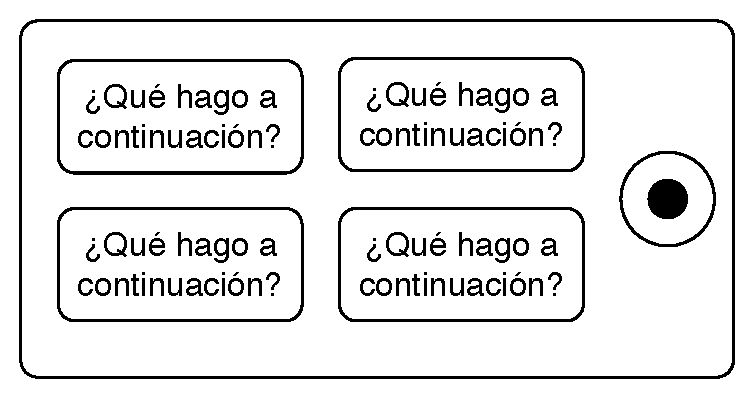
\includegraphics[keepaspectratio,alt={Personal Digital Assistant},height=1.0in]{../images/pda.eps}}
\caption{Personal Digital Assistant}
\end{figure}

Ang mga programmers ay nagdadagdag ng operating system at isang set ng
applications sa hardware at napupunta tayo sa Personal Digital Assistant
na napaka helpful at capable na tumulong sa atin na gumawa ng maraming
iba't ibang bagay.

Ang ating mga computers ay mabilis at may malawak na memory at maaaring
maging napaka helpful sa atin kung alam lang natin ang language na
sasabihin para ipaliwanag sa computer kung ano ang gusto nating ``gawin
next''. Kung alam natin ang language na ito, maaari nating sabihin sa
computer na gawin ang mga tasks para sa atin na repetitive.
Kapansin-pansin, ang mga bagay na kaya ng computers na gawin ay madalas
ang mga bagay na nakakabagot at mind-numbing para sa atin na mga tao.

Halimbawa, tingnan ang unang tatlong paragraphs ng chapter na ito at
sabihin mo sa akin ang pinaka-commonly used na salita at ilang beses
ginamit ang salita. Habang nakaya mong basahin at maintindihan ang mga
salita sa ilang segundo, ang pagbilang sa kanila ay halos masakit dahil
hindi ito ang uri ng problema na idinisenyo ng human minds na
solusyonan. Para sa computer, ang kabaligtaran ang totoo, ang pagbasa at
pag-intindi ng text mula sa papel ay mahirap para sa computer na gawin
pero ang pagbilang ng mga salita at pagsasabi sa iyo kung ilang beses
ang pinaka-ginamit na salita ay napakadali para sa computer:

\begin{Shaded}
\begin{Highlighting}[]
\NormalTok{python words.py}
\NormalTok{Ilagay ang }\BuiltInTok{file}\NormalTok{: words.txt}
\NormalTok{to }\DecValTok{16}
\end{Highlighting}
\end{Shaded}

Ang ating ``personal information analysis assistant'' ay mabilis na
nagsabi sa atin na ang salitang ``to'' ay ginamit ng labing-anim na
beses sa unang tatlong paragraphs ng chapter na ito.

Ang katotohanang ito na ang computers ay magaling sa mga bagay na hindi
kaya ng mga tao ay dahilan kung bakit kailangan mong maging skilled sa
pagsasalita ng ``computer language''. Kapag natutunan mo ang bagong
language na ito, maaari mong idelegate ang mundane tasks sa iyong
partner (ang computer), na nag-iiwan ng mas maraming oras para sa iyo na
gawin ang mga bagay na ikaw lang ang uniquely suited para gawin.
Nagdadala ka ng creativity, intuition, at inventiveness sa partnership
na ito.

\section{Creativity and motivation}\label{creativity-and-motivation}

Habang ang librong ito ay hindi intended para sa professional
programmers, ang professional programming ay maaaring maging
napaka-rewarding na trabaho pareho sa financially at personally. Ang
paggawa ng useful, elegant, at clever programs para sa iba na gamitin ay
isang napaka-creative na activity. Ang iyong computer o Personal Digital
Assistant (PDA) ay karaniwang naglalaman ng maraming iba't ibang
programs mula sa maraming iba't ibang grupo ng programmers, bawat isa ay
nakikipag-compete para sa iyong attention at interest. Sinusubukan nila
ang kanilang makakaya para matugunan ang iyong pangangailangan at bigyan
ka ng great user experience sa proseso. Sa ilang situations, kapag
pumili ka ng piece ng software, ang mga programmers ay direktang
compensated dahil sa iyong choice.

Kung iisipin natin ang programs bilang creative output ng mga grupo ng
programmers, marahil ang sumusunod na figure ay mas sensible na version
ng ating PDA:

\begin{figure}
\centering
\pandocbounded{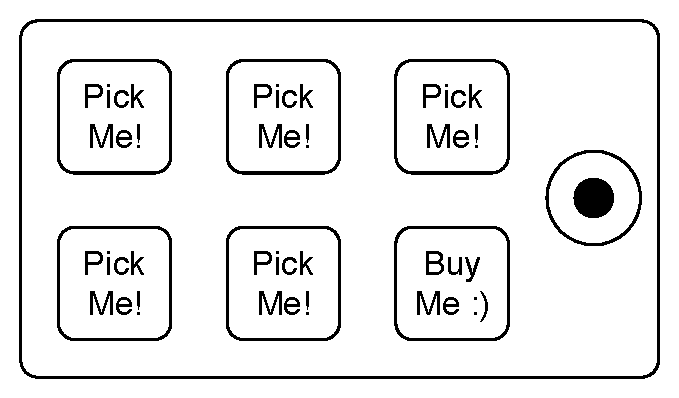
\includegraphics[keepaspectratio,alt={Programmers Talking to You},height=1.0in]{../images/pda2.eps}}
\caption{Programmers Talking to You}
\end{figure}

Sa ngayon, ang ating primary motivation ay hindi para kumita o
mag-please sa end users, kundi para sa atin na maging mas productive sa
pag-handle ng data at information na makakaharap natin sa ating buhay.
Kapag nagsimula ka, ikaw ay pareho ang programmer at ang end user ng
iyong programs. Habang nakakakuha ka ng skill bilang programmer at ang
programming ay mas naging creative sa iyo, ang iyong mga iniisip ay
maaaring mag-turn patungo sa pag-develop ng programs para sa iba.

\section{Computer hardware
architecture}\label{computer-hardware-architecture}

\index{hardware} \index{hardware!architecture}

Bago tayo magsimula matuto ng language na sinasabi natin para magbigay
ng instructions sa computers para mag-develop ng software, kailangan
nating matuto ng kaunti tungkol sa kung paano ginawa ang computers. Kung
kukunin mo ang iyong computer o cell phone at titingnan nang malalim sa
loob, makikita mo ang sumusunod na parts:

\begin{figure}
\centering
\pandocbounded{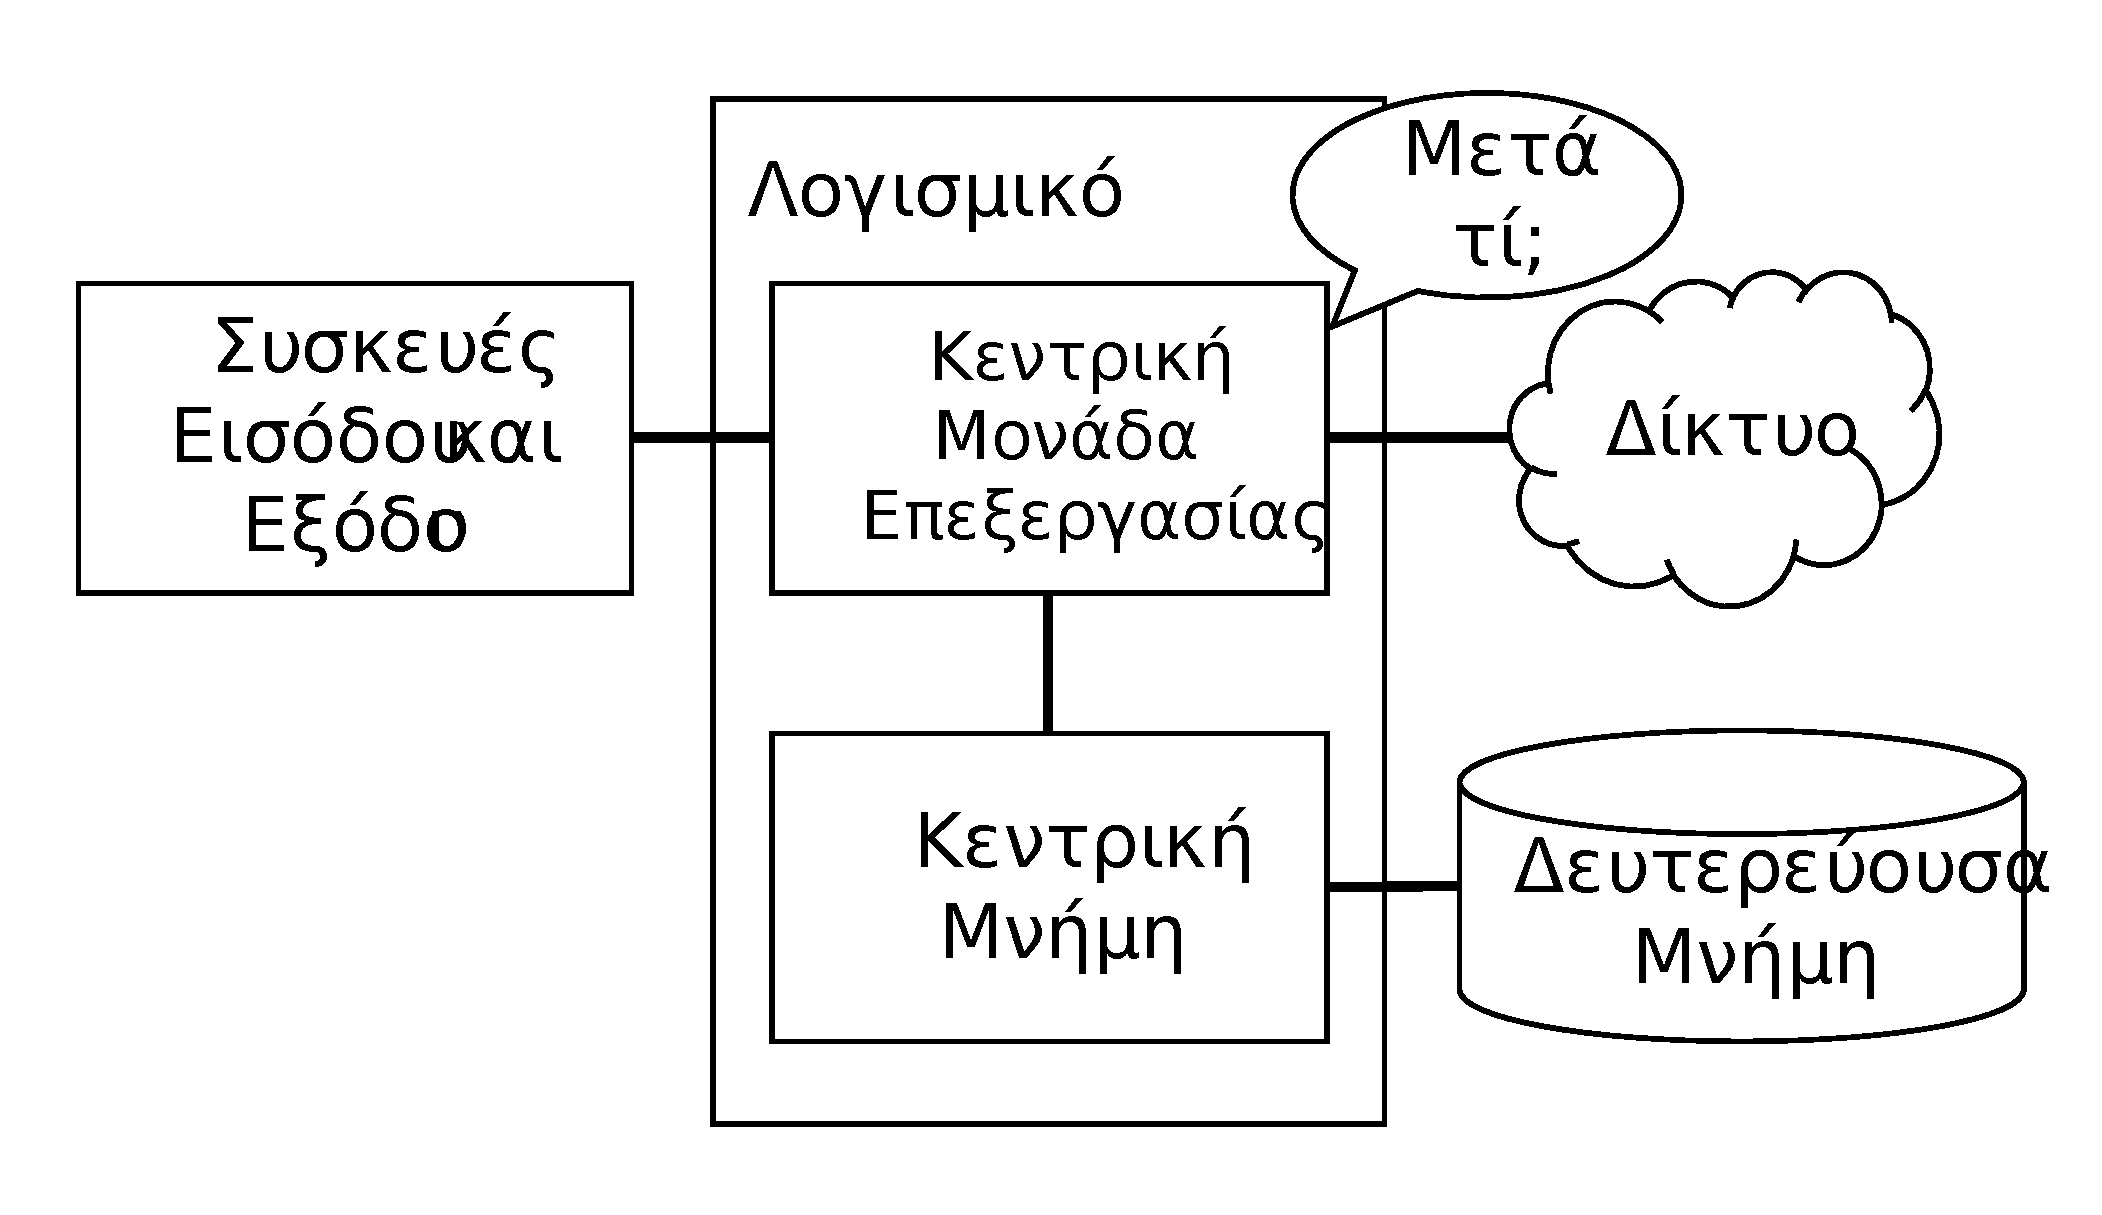
\includegraphics[keepaspectratio,alt={Hardware Architecture},height=1.75in]{../images/arch.eps}}
\caption{Hardware Architecture}
\end{figure}

Ang high-level definitions ng mga parts na ito ay ang sumusunod:

\begin{itemize}
\item
  Ang \emph{Central Processing Unit} (o CPU) ay ang parte ng computer na
  ginawa para maging obsessed sa ``ano ang next?'' Kung ang iyong
  computer ay rated sa 3.0 Gigahertz, ibig sabihin ang CPU ay
  magtatanong ng ``What next?'' tatlong bilyong beses kada segundo.
  Kailangan mong matutunan kung paano magsalita nang mabilis para
  makasabay sa CPU.
\item
  Ang \emph{Main Memory} ay ginagamit para mag-store ng information na
  kailangan ng CPU nang mabilis. Ang main memory ay halos kasing bilis
  ng CPU. Pero ang information na naka-store sa main memory ay nawawala
  kapag ang computer ay naka-off.
\item
  Ang \emph{Secondary Memory} ay ginagamit din para mag-store ng
  information, pero mas mabagal ito kaysa sa main memory. Ang advantage
  ng secondary memory ay maaari itong mag-store ng information kahit
  walang power ang computer. Mga halimbawa ng secondary memory ay disk
  drives o flash memory (karaniwang matatagpuan sa USB sticks at
  portable music players).
\item
  Ang \emph{Input and Output Devices} ay simpleng ating screen,
  keyboard, mouse, microphone, speaker, touchpad, etc. Sila ang lahat ng
  paraan kung paano tayo nakikipag-interact sa computer.
\item
  Sa panahon ngayon, karamihan ng computers ay mayroon ding
  \emph{Network Connection} para mag-retrieve ng information sa network.
  Maaari nating isipin ang network bilang napakabagal na lugar para
  mag-store at mag-retrieve ng data na maaaring hindi palaging ``up''.
  Kaya sa isang paraan, ang network ay isang mas mabagal at kung minsan
  unreliable na form ng \emph{Secondary Memory}.
\end{itemize}

Habang karamihan ng detalye kung paano gumagana ang mga components na
ito ay mas mabuting iwanan sa computer builders, nakakatulong na mayroon
tayong ilang terminology para makapag-usap tayo tungkol sa mga iba't
ibang parts na ito habang sumusulat tayo ng ating programs.

Bilang programmer, ang trabaho mo ay gamitin at i-orchestrate ang bawat
isa sa mga resources na ito para solusyonan ang problema na kailangan
mong solusyonan at i-analyze ang data na makukuha mo mula sa solusyon.
Bilang programmer ay kadalasan mong ``kakausapin'' ang CPU at sasabihin
mo sa kanya kung ano ang gagawin next. Minsan ay sasabihin mo sa CPU na
gamitin ang main memory, secondary memory, network, o ang input/output
devices.

\begin{figure}
\centering
\pandocbounded{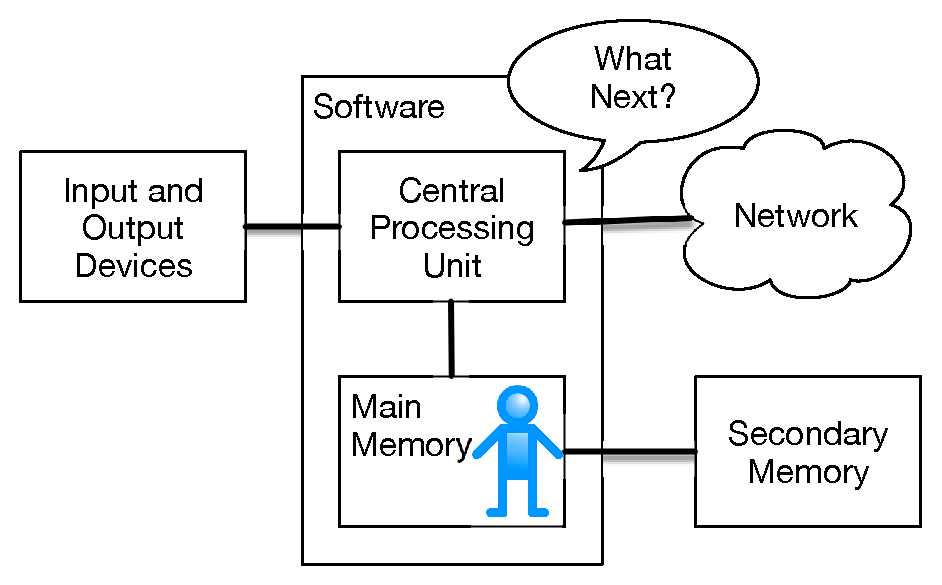
\includegraphics[keepaspectratio,alt={Where Are You?},height=1.75in]{../images/arch2.eps}}
\caption{Where Are You?}
\end{figure}

Kailangan mong maging tao na sumasagot sa tanong ng CPU na ``What
next?'' Pero magiging napaka-uncomfortable na paliitin ka sa 5mm ang
taas at ipasok ka sa computer para lang makapag-issue ka ng command na
tatlong bilyong beses kada segundo. Kaya sa halip, kailangan mong isulat
ang iyong instructions in advance. Tinatawag natin ang mga stored
instructions na ito bilang \emph{program} at ang gawain ng pagsusulat ng
mga instructions na ito at paggawa ng mga instructions na tama ay
\emph{programming}.

\section{Understanding programming}\label{understanding-programming}

Sa natitirang bahagi ng librong ito, susubukan naming gawin kang tao na
skilled sa art ng programming. Sa huli ay magiging isa kang
\emph{programmer} - marahil hindi professional programmer, pero hindi
bababa ay magkakaroon ka ng skills para tingnan ang data/information
analysis problem at mag-develop ng program para solusyonan ang problema.

\index{problem solving}

Sa isang paraan, kailangan mo ng dalawang skills para maging programmer:

\begin{itemize}
\item
  Una, kailangan mong malaman ang programming language (Python) -
  kailangan mong malaman ang vocabulary at ang grammar. Kailangan mong
  makapag-spell ng mga salita sa bagong language na ito nang tama at
  malaman kung paano gumawa ng well-formed na ``sentences'' sa bagong
  language na ito.
\item
  Pangalawa, kailangan mong ``mag-kwento''. Sa pagsusulat ng kwento,
  pinagsasama mo ang mga salita at sentences para iparating ang ideya sa
  reader. Mayroong skill at art sa paggawa ng kwento, at ang skill sa
  story writing ay napapabuti sa pamamagitan ng pagsusulat at pagkuha ng
  feedback. Sa programming, ang ating program ay ang ``kwento'' at ang
  problema na sinusubukan mong solusyonan ay ang ``ideya''.
\end{itemize}

Kapag natutunan mo ang isang programming language tulad ng Python, mas
madali mong matututunan ang pangalawang programming language tulad ng
JavaScript o C++. Ang bagong programming language ay may napaka-ibang
vocabulary at grammar pero ang problem-solving skills ay pareho sa lahat
ng programming languages.

Matututunan mo ang ``vocabulary'' at ``sentences'' ng Python nang medyo
mabilis. Mas matagal bago mo makaya na sumulat ng coherent program para
solusyonan ang brand-new problem. Tinuturo namin ang programming katulad
ng pagtuturo namin ng writing. Nagsisimula tayo sa pagbasa at
pagpapaliwanag ng programs, pagkatapos sumusulat tayo ng simple
programs, at pagkatapos sumusulat tayo ng mas kumplikadong programs sa
paglipas ng panahon. Sa ilang punto ay ``makukuha mo ang iyong muse'' at
makikita mo ang patterns sa sarili mo at mas natural mong makikita kung
paano kumuha ng problema at sumulat ng program na solusyonan ang
problemang iyon. At kapag nakarating ka na sa puntong iyon, ang
programming ay nagiging napaka-pleasant at creative na proseso.

Nagsisimula tayo sa vocabulary at structure ng Python programs. Maging
patient habang ang simple examples ay nagpapaalala sa iyo ng noong
nagsimula kang magbasa sa unang pagkakataon.

\section{Words and sentences}\label{words-and-sentences}

\index{programming language} \index{reserved words}
\index{language!programming} \index{keywords}

Hindi tulad ng human languages, ang Python vocabulary ay talagang medyo
maliit. Tinatawag natin ang ``vocabulary'' na ito bilang ``reserved
words'' o ``keywords''. Ang mga salitang ito ay may napaka-espesyal na
kahulugan para sa Python. Kapag nakikita ng Python ang mga salitang ito
sa isang Python program, mayroon silang isa at tanging isang kahulugan
para sa Python. Mamaya habang sumusulat ka ng programs ay gagawa ka ng
sarili mong mga salita na may kahulugan para sa iyo na tinatawag na
\emph{variables}. Magkakaroon ka ng malaking kalayaan sa pagpili ng mga
pangalan para sa iyong variables, pero hindi mo maaaring gamitin ang
alinman sa reserved words ng Python bilang pangalan ng variable.

Kapag nagte-train tayo ng aso, gumagamit tayo ng espesyal na salita
tulad ng ``sit'', ``stay'', at ``fetch''. Kapag nakikipag-usap ka sa aso
at hindi gumagamit ng alinman sa reserved words, titingin lang sila sa
iyo na may quizzical look sa kanilang mukha hanggang sabihin mo ang
isang reserved word. Halimbawa, kung sasabihin mo, ``I wish more people
would walk to improve their overall health'', ang marahil na naririnig
ng karamihan ng aso ay, ``blah blah blah \emph{walk} blah blah blah
blah.'' Iyon ay dahil ang ``walk'' ay isang reserved word sa dog
language. Marami ang maaaring magsabi na ang language sa pagitan ng mga
tao at pusa ay walang reserved words\footnote{\url{http://xkcd.com/231/}}.

Ang mga reserved words sa language kung saan nakikipag-usap ang mga tao
sa Python ay kasama ang sumusunod:

{\small
\begin{verbatim}
False      await      else       import     pass
None       break      except     in         raise
True       class      finally    is         return
and        continue   for        lambda     try
as         def        from       nonlocal   while
assert     del        global     not        with
async      elif       if         or         yield
\end{verbatim}
}

Iyon lang, at hindi tulad ng aso, ang Python ay ganap na trained na.
Kapag sinabi mo ang ``try'', susubukan ng Python tuwing sasabihin mo ito
nang walang pagkakamali.

Matututunan natin ang mga reserved words na ito at kung paano sila
ginagamit sa tamang panahon, pero sa ngayon ay tututukan natin ang
Python equivalent ng ``speak'' (sa human-to-dog language). Ang maganda
sa pagsasabi sa Python na magsalita ay maaari pa nating sabihin sa kanya
kung ano ang sasabihin sa pamamagitan ng pagbibigay ng mensahe sa
quotes:

\begin{Shaded}
\begin{Highlighting}[]
\BuiltInTok{print}\NormalTok{(}\StringTok{\textquotesingle{}Hello world!\textquotesingle{}}\NormalTok{)}
\end{Highlighting}
\end{Shaded}

At nakasulat na natin ang ating unang syntactically correct na Python
sentence. Ang ating sentence ay nagsisimula sa function na \emph{print}
na sinusundan ng string ng text na ating pinili na nakapaloob sa single
quotes. Ang mga strings sa print statements ay nakapaloob sa quotes. Ang
single quotes at double quotes ay pareho ang ginagawa; karamihan ng tao
ay gumagamit ng single quotes maliban sa mga kaso kung saan ang single
quote (na apostrophe din) ay lumalabas sa string.

\section{Conversing with Python}\label{conversing-with-python}

Ngayon na mayroon na tayong salita at simpleng sentence na alam natin sa
Python, kailangan nating malaman kung paano magsimula ng conversation sa
Python para i-test ang ating bagong language skills.

Bago ka makapag-converse sa Python, kailangan mo munang i-install ang
Python software sa iyong computer at matutunan kung paano magsimula ng
Python sa iyong computer. Masyadong maraming detalye iyon para sa
chapter na ito kaya iminumungkahi ko na konsultahin mo ang
\href{http://www.py4e.com}{www.py4e.com} kung saan mayroon akong
detailed instructions at screencasts ng pag-setup at pag-start ng Python
sa Macintosh at Windows systems. Sa ilang punto, ikaw ay nasa terminal o
command window at magta-type ka ng \emph{python} at ang Python
interpreter ay magsisimulang mag-execute sa interactive mode at lalabas
na medyo ganito:

\index{interactive mode}

\begin{Shaded}
\begin{Highlighting}[]
\NormalTok{Python }\FloatTok{3.11.6}\NormalTok{ (main, Nov  }\DecValTok{2} \DecValTok{2023}\NormalTok{, }\DecValTok{0}\ErrorTok{4}\NormalTok{:}\DecValTok{39}\NormalTok{:}\DecValTok{43}\NormalTok{) }
\NormalTok{   [Clang }\FloatTok{14.0.3}\NormalTok{ (clang}\OperatorTok{{-}}\FloatTok{1403.0.22.14.1}\NormalTok{)] on darwin}
\NormalTok{Type }\StringTok{"help"}\NormalTok{, }\StringTok{"copyright"}\NormalTok{, }\StringTok{"credits"} \KeywordTok{or} \StringTok{"license"} \ControlFlowTok{for}\NormalTok{ more}
\NormalTok{information.}
\OperatorTok{\textgreater{}\textgreater{}\textgreater{}}
\end{Highlighting}
\end{Shaded}

Ang \texttt{\textgreater{}\textgreater{}\textgreater{}} prompt ay ang
paraan ng Python interpreter na magtanong sa iyo, ``Ano ang gusto mong
gawin ko next?'' Handa na ang Python na makipag-converse sa iyo. Ang
kailangan mo lang malaman ay kung paano magsalita ng Python language.

Sabihin natin halimbawa na hindi mo alam kahit ang pinakasimpleng Python
language words o sentences. Maaaring gusto mong gamitin ang standard
line na ginagamit ng mga astronauts kapag lumapag sila sa malayong
planeta at sinusubukan nilang makipag-usap sa mga naninirahan sa
planeta:

\begin{Shaded}
\begin{Highlighting}[]
\OperatorTok{\textgreater{}\textgreater{}\textgreater{}}\NormalTok{ I come }\KeywordTok{in}\NormalTok{ peace, please take me to your leader}
\NormalTok{File }\StringTok{"\textless{}stdin\textgreater{}"}\NormalTok{, line }\DecValTok{1}
\NormalTok{    I come }\KeywordTok{in}\NormalTok{ peace take me tou your leader}
      \OperatorTok{\^{}\^{}\^{}\^{}}
\PreprocessorTok{SyntaxError}\NormalTok{: invalid syntax}
\OperatorTok{\textgreater{}\textgreater{}\textgreater{}}
\end{Highlighting}
\end{Shaded}

Hindi masyadong maayos ito. Maliban kung may maisip ka agad, ang mga
naninirahan sa planeta ay malamang na tutusukin ka ng kanilang mga
sibat, ilalagay ka sa tuhog, iihawin ka sa apoy, at kakainin ka para sa
hapunan.

Swerteng dala mo ang kopya ng librong ito sa iyong paglalakbay, at
binuksan mo ang pahinang ito at sinubukan mo ulit:

\begin{Shaded}
\begin{Highlighting}[]
\OperatorTok{\textgreater{}\textgreater{}\textgreater{}} \BuiltInTok{print}\NormalTok{(}\StringTok{\textquotesingle{}Hello world!\textquotesingle{}}\NormalTok{)}
\NormalTok{Hello world}\OperatorTok{!}
\end{Highlighting}
\end{Shaded}

Mas maayos na ito, kaya sinubukan mong makipag-communicate pa:

\begin{Shaded}
\begin{Highlighting}[]
\OperatorTok{\textgreater{}\textgreater{}\textgreater{}} \BuiltInTok{print}\NormalTok{(}\StringTok{\textquotesingle{}You must be the legendary god that comes from the sky\textquotesingle{}}\NormalTok{)}
\NormalTok{You must be the legendary god that comes }\ImportTok{from}\NormalTok{ the sky}
\OperatorTok{\textgreater{}\textgreater{}\textgreater{}} \BuiltInTok{print}\NormalTok{(}\StringTok{\textquotesingle{}We have been waiting for you for a long time\textquotesingle{}}\NormalTok{)}
\NormalTok{We have been waiting }\ControlFlowTok{for}\NormalTok{ you }\ControlFlowTok{for}\NormalTok{ a }\BuiltInTok{long}\NormalTok{ time}
\OperatorTok{\textgreater{}\textgreater{}\textgreater{}} \BuiltInTok{print}\NormalTok{(}\StringTok{\textquotesingle{}Our legend says you will be very tasty with mustard\textquotesingle{}}\NormalTok{)}
\NormalTok{Our legend says you will be very tasty }\ControlFlowTok{with}\NormalTok{ mustard}
\OperatorTok{\textgreater{}\textgreater{}\textgreater{}} \BuiltInTok{print} \StringTok{\textquotesingle{}We will have a feast tonight unless you say}
\ErrorTok{  File "\textless{}stdin\textgreater{}", line 1}
    \BuiltInTok{print} \StringTok{\textquotesingle{}We will have a feast tonight unless you say}
\ErrorTok{          \^{}}
\PreprocessorTok{SyntaxError}\NormalTok{: unterminated string literal (detected at line }\DecValTok{1}\NormalTok{)}
\OperatorTok{\textgreater{}\textgreater{}\textgreater{}}
\end{Highlighting}
\end{Shaded}

Ang conversation ay maayos nang sandali at pagkatapos gumawa ka ng
pinakamaliit na pagkakamali sa paggamit ng Python language at ibinalik
ng Python ang mga sibat.

Sa puntong ito, dapat mo ring mapagtanto na habang ang Python ay napaka
complex at powerful at napaka-picky tungkol sa syntax na ginagamit mo
para makipag-communicate dito, ang Python ay \emph{hindi} intelligent.
Ikaw ay talagang nakikipag-converse lang sa sarili mo, pero gumagamit ng
proper syntax.

Sa isang paraan, kapag gumagamit ka ng program na sinulat ng iba, ang
conversation ay sa pagitan mo at ng mga programmer na iyon na may Python
na nagsisilbing intermediary. Ang Python ay paraan para sa mga creators
ng programs na ipahayag kung paano dapat magpatuloy ang conversation. At
sa ilang chapters pa lang, ikaw ay magiging isa sa mga programmer na
iyon na gumagamit ng Python para makipag-usap sa mga users ng iyong
program.

Bago tayo umalis sa ating unang conversation sa Python interpreter,
dapat mong malaman ang tamang paraan na sabihin ang ``good-bye'' kapag
nakikipag-interact sa mga naninirahan sa Planet Python:

\begin{Shaded}
\begin{Highlighting}[]
\OperatorTok{\textgreater{}\textgreater{}\textgreater{}}\NormalTok{ good}\OperatorTok{{-}}\NormalTok{bye}
\NormalTok{Traceback (most recent call last):}
\NormalTok{  File }\StringTok{"\textless{}stdin\textgreater{}"}\NormalTok{, line }\DecValTok{1}\NormalTok{, }\KeywordTok{in} \OperatorTok{\textless{}}\NormalTok{module}\OperatorTok{\textgreater{}}
\PreprocessorTok{NameError}\NormalTok{: name }\StringTok{\textquotesingle{}good\textquotesingle{}} \KeywordTok{is} \KeywordTok{not}\NormalTok{ defined}
\OperatorTok{\textgreater{}\textgreater{}\textgreater{}} \ControlFlowTok{if}\NormalTok{ you don}\StringTok{\textquotesingle{}t mind, I need to leave}
\ErrorTok{  File "\textless{}stdin\textgreater{}", line 1}
    \ControlFlowTok{if}\NormalTok{ you don}\StringTok{\textquotesingle{}t mind, I need to leave}
\ErrorTok{              \^{}}
\PreprocessorTok{SyntaxError}\NormalTok{: unterminated string literal (detected at line }\DecValTok{1}\NormalTok{)}
\OperatorTok{\textgreater{}\textgreater{}\textgreater{}}\NormalTok{ quit()}
\end{Highlighting}
\end{Shaded}

Mapapansin mo na ang error ay iba para sa unang dalawang incorrect
attempts. Ang pangalawang error ay iba dahil ang \emph{if} ay isang
reserved word at nakita ng Python ang reserved word at naisip na
sinusubukan nating sabihin ang isang bagay pero mali ang syntax ng
sentence.

Ang tamang paraan na sabihin ang ``good-bye'' sa Python ay i-enter ang
\emph{quit()} sa interactive chevron na
\texttt{\textgreater{}\textgreater{}\textgreater{}} prompt. Malamang ay
matagal mong hulaan iyon, kaya ang pagkakaroon ng libro na malapit ay
malamang na makakatulong.

\section{Terminology: Interpreter and
compiler}\label{terminology-interpreter-and-compiler}

Ang Python ay isang \emph{high-level} language na intended na maging
relatively straightforward para sa mga tao na basahin at isulat at para
sa computers na basahin at i-process. Ang iba pang high-level languages
ay kasama ang Java, C++, PHP, Ruby, Basic, Perl, JavaScript, at marami
pa. Ang actual hardware sa loob ng Central Processing Unit (CPU) ay
hindi naiintindihan ang alinman sa mga high-level languages na ito.

Ang CPU ay naiintindihan ang language na tinatawag nating \emph{machine
language}. Ang machine language ay napaka-simple at totoo lang napaka
nakakapagod na isulat dahil ito ay kinakatawan lahat sa zeros at ones:

{\small
\begin{verbatim}
001010001110100100101010000001111
11100110000011101010010101101101
...
\end{verbatim}
}

Ang machine language ay mukhang medyo simple sa surface, dahil mayroon
lang zeros at ones, pero ang syntax nito ay mas complex pa at mas
intricate kaysa sa Python. Kaya kakaunti lang ang programmers na
sumusulat ng machine language. Sa halip ay gumagawa tayo ng iba't ibang
translators para payagan ang mga programmers na sumulat sa high-level
languages tulad ng Python o JavaScript at ang mga translators na ito ay
nagko-convert ng programs sa machine language para sa actual execution
ng CPU.

Dahil ang machine language ay nakatali sa computer hardware, ang machine
language ay hindi \emph{portable} sa iba't ibang uri ng hardware. Ang
mga programs na sinulat sa high-level languages ay maaaring ilipat sa
pagitan ng iba't ibang computers sa pamamagitan ng paggamit ng ibang
interpreter sa bagong machine o pag-recompile ng code para gumawa ng
machine language version ng program para sa bagong machine.

Ang mga programming language translators na ito ay nahahati sa dalawang
general categories: (1) interpreters at (2) compilers.

Ang \emph{interpreter} ay nagbabasa ng source code ng program na sinulat
ng programmer, nagpa-parse ng source code, at nag-i-interpret ng
instructions on the fly. Ang Python ay isang interpreter at kapag
nagpapatakbo tayo ng Python interactively, maaari tayong mag-type ng
linya ng Python (isang sentence) at agad na i-process ng Python ito at
handa na para sa atin na mag-type ng iba pang linya ng Python.

Ang ilan sa mga linya ng Python ay nagsasabi sa Python na gusto mong
tandaan nito ang ilang value para mamaya. Kailangan nating pumili ng
pangalan para sa value na iyon para matandaan at maaari nating gamitin
ang symbolic name na iyon para i-retrieve ang value mamaya. Ginagamit
natin ang term na \emph{variable} para tumukoy sa mga labels na
ginagamit natin para tumukoy sa stored data na ito.

\begin{Shaded}
\begin{Highlighting}[]
\OperatorTok{\textgreater{}\textgreater{}\textgreater{}}\NormalTok{ x }\OperatorTok{=} \DecValTok{6}
\OperatorTok{\textgreater{}\textgreater{}\textgreater{}} \BuiltInTok{print}\NormalTok{(x)}
\DecValTok{6}
\OperatorTok{\textgreater{}\textgreater{}\textgreater{}}\NormalTok{ y }\OperatorTok{=}\NormalTok{ x }\OperatorTok{*} \DecValTok{7}
\OperatorTok{\textgreater{}\textgreater{}\textgreater{}} \BuiltInTok{print}\NormalTok{(y)}
\DecValTok{42}
\OperatorTok{\textgreater{}\textgreater{}\textgreater{}}
\end{Highlighting}
\end{Shaded}

Sa halimbawang ito, hinihiling natin sa Python na tandaan ang value na
anim at gamitin ang label na \emph{x} para ma-retrieve natin ang value
mamaya. Sinusuri natin na talagang naalala ng Python ang value sa
pamamagitan ng paggamit ng \emph{print}. Pagkatapos hinihiling natin sa
Python na i-retrieve ang \emph{x} at i-multiply ito sa pito at ilagay
ang bagong computed value sa \emph{y}. Pagkatapos hinihiling natin sa
Python na i-print ang value na kasalukuyang nasa \emph{y}.

Kahit na nagta-type tayo ng mga commands na ito sa Python isa-isa,
tinatrato ng Python ang mga ito bilang ordered sequence ng statements na
ang mga susunod na statements ay makakakuha ng data na ginawa sa naunang
statements. Sumusulat tayo ng ating unang simpleng paragraph na may apat
na sentences sa logical at meaningful na order.

Ito ang kalikasan ng \emph{interpreter} na makapagkaroon ng interactive
conversation tulad ng ipinakita sa itaas. Ang \emph{compiler} ay
kailangan ng buong program sa isang file, at pagkatapos nagpapatakbo ito
ng process para i-translate ang high-level source code sa machine
language at pagkatapos inilalagay ng compiler ang resulting machine
language sa isang file para sa execution mamaya.

Kung mayroon kang Windows system, kadalasan ang mga executable machine
language programs na ito ay may suffix na ``.exe'' o ``.dll'' na
nangangahulugang ``executable'' at ``dynamic link library'' ayon sa
pagkakabanggit. Sa Linux at Macintosh, walang suffix na natatanging
nagmamarka sa file bilang executable.

Kung bubuksan mo ang executable file sa text editor, mukha itong ganap
na kakaiba at hindi mabasa:

{\small
\begin{verbatim}
^?ELF^A^A^A^@^@^@^@^@^@^@^@^@^B^@^C^@^A^@^@^@\xa0\x82
^D^H4^@^@^@\x90^]^@^@^@^@^@^@4^@ ^@^G^@(^@$^@!^@^F^@
^@^@4^@^@^@4\x80^D^H4\x80^D^H\xe0^@^@^@\xe0^@^@^@^E
^@^@^@^D^@^@^@^C^@^@^@^T^A^@^@^T\x81^D^H^T\x81^D^H^S
^@^@^@^S^@^@^@^D^@^@^@^A^@^@^@^A\^D^HQVhT\x83^D^H\xe8
....
\end{verbatim}
}

Hindi madaling basahin o isulat ang machine language, kaya maganda na
mayroon tayong \emph{interpreters} at \emph{compilers} na
nagpapahintulot sa atin na sumulat sa high-level languages tulad ng
Python o C.

Ngayon sa puntong ito sa ating discussion tungkol sa compilers at
interpreters, dapat ay nagtataka ka ng kaunti tungkol sa Python
interpreter mismo. Sa anong language ito sinulat? Sinulat ba ito sa
compiled language? Kapag nagta-type tayo ng ``python'', ano talaga ang
nangyayari?

Ang Python interpreter ay sinulat sa high-level language na tinatawag na
``C''. Maaari mong tingnan ang actual source code para sa Python
interpreter sa pamamagitan ng pagpunta sa
\href{http://www.python.org}{www.python.org} at pag-navigate sa kanilang
source code. Kaya ang Python ay program mismo at ito ay na-compile sa
machine code. Kapag nag-install ka ng Python sa iyong computer (o ang
vendor ang nag-install nito), kinopya mo ang machine-code copy ng
translated Python program sa iyong system. Sa Windows, ang executable
machine code para sa Python mismo ay malamang nasa file na may pangalan
tulad ng:

{\small
\begin{verbatim}
C:\Python35\python.exe
\end{verbatim}
}

Iyon ay higit pa sa kailangan mong malaman para maging Python
programmer, pero minsan ay nakakatulong na sagutin ang mga maliit na
nakakabagot na tanong sa simula pa lang.

\section{Writing a program}\label{writing-a-program}

Ang pagta-type ng commands sa Python interpreter ay magandang paraan
para mag-experiment sa features ng Python, pero hindi ito inirerekomenda
para solusyonan ang mas complex problems.

Kapag gusto nating sumulat ng program, gumagamit tayo ng text editor
para isulat ang Python instructions sa isang file, na tinatawag na
\emph{script}. Ayon sa convention, ang Python scripts ay may mga
pangalan na nagtatapos sa \texttt{.py}.

\index{script}

Para i-execute ang script, kailangan mong sabihin sa Python interpreter
ang pangalan ng file. Sa command window, magta-type ka ng
\texttt{python\ hello.py} tulad ng sumusunod:

\begin{Shaded}
\begin{Highlighting}[]
\ExtensionTok{$}\NormalTok{ cat hello.py}
\ExtensionTok{print}\ErrorTok{(}\StringTok{\textquotesingle{}Hello world!\textquotesingle{}}\KeywordTok{)}
\ExtensionTok{$}\NormalTok{ python hello.py}
\ExtensionTok{Hello}\NormalTok{ world!}
\end{Highlighting}
\end{Shaded}

Ang ``\$'' ay ang operating system prompt, at ang ``cat hello.py'' ay
nagpapakita sa atin na ang file na ``hello.py'' ay may one-line Python
program para mag-print ng string.

Tinatawag natin ang Python interpreter at sinasabi natin sa kanya na
basahin ang source code mula sa file na ``hello.py'' imbes na mag-prompt
sa atin para sa mga linya ng Python code interactively.

Mapapansin mo na hindi kailangan na mayroong \emph{quit()} sa dulo ng
Python program sa file. Kapag nagbabasa ang Python ng iyong source code
mula sa file, alam nito na huminto kapag naabot na ang dulo ng file.

\section{What is a program?}\label{what-is-a-program}

Ang definition ng \emph{program} sa pinakabasikong antas ay isang
sequence ng Python statements na ginawa para gumawa ng isang bagay.
Kahit ang ating simpleng \emph{hello.py} script ay isang program. Ito ay
isang one-line program at hindi partikular na useful, pero sa strictest
definition, ito ay isang Python program.

Maaaring pinakamadaling maintindihan kung ano ang program sa pamamagitan
ng pag-iisip tungkol sa isang problema na maaaring gawin ng program para
solusyonan, at pagkatapos tingnan ang isang program na solusyonan ang
problemang iyon.

Sabihin natin na gumagawa ka ng Social Computing research sa Facebook
posts at interesado ka sa pinaka-frequently used na salita sa isang
serye ng posts. Maaari mong i-print ang stream ng Facebook posts at
pag-aralan ang text na hinahanap ang pinaka-common na salita, pero
magtatagal iyon at napaka-prone sa pagkakamali. Magiging matalino ka
kung susulat ka ng Python program para gawin ang task nang mabilis at
tumpak para magawa mo ang weekend sa paggawa ng masaya.

Halimbawa, tingnan ang sumusunod na text tungkol sa isang clown at
kotse. Tingnan ang text at alamin ang pinaka-common na salita at ilang
beses ito nangyari.

{\small
\begin{verbatim}
the clown ran after the car and the car ran into the tent
and the tent fell down on the clown and the car
\end{verbatim}
}

Pagkatapos isipin na ginagawa mo ang task na ito na tumitingin sa
milyun-milyong linya ng text. Totoo lang mas mabilis para sa iyo na
matutunan ang Python at sumulat ng Python program para bilangin ang mga
salita kaysa sa manually i-scan ang mga salita.

Ang mas magandang balita ay mayroon na akong simpleng program para
hanapin ang pinaka-common na salita sa text file. Sinulat ko ito,
na-test ko ito, at ngayon ibinibigay ko ito sa iyo para gamitin para
makatipid ka ng oras.

\begin{Shaded}
\begin{Highlighting}[]
\NormalTok{name }\OperatorTok{=} \BuiltInTok{input}\NormalTok{(}\StringTok{\textquotesingle{}Enter file: \textquotesingle{}}\NormalTok{)}
\NormalTok{handle }\OperatorTok{=} \BuiltInTok{open}\NormalTok{(name, }\StringTok{\textquotesingle{}r\textquotesingle{}}\NormalTok{)}
\NormalTok{counts }\OperatorTok{=} \BuiltInTok{dict}\NormalTok{()}

\ControlFlowTok{for}\NormalTok{ line }\KeywordTok{in}\NormalTok{ handle:}
\NormalTok{    words }\OperatorTok{=}\NormalTok{ line.split()}
    \ControlFlowTok{for}\NormalTok{ word }\KeywordTok{in}\NormalTok{ words:}
\NormalTok{        counts[word] }\OperatorTok{=}\NormalTok{ counts.get(word, }\DecValTok{0}\NormalTok{) }\OperatorTok{+} \DecValTok{1}

\NormalTok{bigcount }\OperatorTok{=} \VariableTok{None}
\NormalTok{bigword }\OperatorTok{=} \VariableTok{None}
\ControlFlowTok{for}\NormalTok{ word, count }\KeywordTok{in} \BuiltInTok{list}\NormalTok{(counts.items()):}
    \ControlFlowTok{if}\NormalTok{ bigcount }\KeywordTok{is} \VariableTok{None} \KeywordTok{or}\NormalTok{ count }\OperatorTok{\textgreater{}}\NormalTok{ bigcount:}
\NormalTok{        bigword }\OperatorTok{=}\NormalTok{ word}
\NormalTok{        bigcount }\OperatorTok{=}\NormalTok{ count}

\BuiltInTok{print}\NormalTok{(bigword, bigcount)}

\CommentTok{\# Code: https://www.py4e.com/code3/words.py}
\end{Highlighting}
\end{Shaded}

\begin{trinketfiles}
../code3/words.txt
\end{trinketfiles}

Hindi mo kailangan na malaman ang Python para gamitin ang program na
ito. Kailangan mong makapagdaan sa Chapter 10 ng librong ito para ganap
na maintindihan ang awesome Python techniques na ginamit para gawin ang
program. Ikaw ang end user, ginagamit mo lang ang program at namamangha
sa cleverness nito at kung paano ito nakatipid sa iyo ng napakaraming
manual effort. Nagta-type ka lang ng code sa isang file na tinatawag na
\emph{words.py} at patakbuhin ito o i-download mo ang source code mula
sa \url{http://www.py4e.com/code3/} at patakbuhin ito.

\index{program}

Ito ay magandang halimbawa kung paano ang Python at ang Python language
ay nagsisilbing intermediary sa pagitan mo (ang end user) at ako (ang
programmer). Ang Python ay paraan para sa atin na magpalitan ng useful
instruction sequences (i.e., programs) sa common language na maaaring
gamitin ng sinuman na nag-install ng Python sa kanilang computer. Kaya
wala sa atin ang nakikipag-usap \emph{sa Python}, sa halip ay
nakikipag-communicate tayo sa isa't isa \emph{sa pamamagitan} ng Python.

\section{The building blocks of
programs}\label{the-building-blocks-of-programs}

Sa susunod na ilang chapters, matututunan natin ang higit pa tungkol sa
vocabulary, sentence structure, paragraph structure, at story structure
ng Python. Matututunan natin ang powerful capabilities ng Python at kung
paano i-compose ang mga capabilities na iyon para gumawa ng useful
programs.

Mayroong ilang low-level conceptual patterns na ginagamit natin para
gumawa ng programs. Ang mga constructs na ito ay hindi lang para sa
Python programs, sila ay parte ng bawat programming language mula sa
machine language hanggang sa high-level languages.

\begin{description}
\tightlist
\item[input]
Kumuha ng data mula sa ``outside world''. Maaari itong pagbasa ng data
mula sa isang file, o kahit ilang uri ng sensor tulad ng microphone o
GPS. Sa ating initial programs, ang ating input ay manggagaling sa user
na nagta-type ng data sa keyboard.
\item[output]
I-display ang results ng program sa screen o i-store ang mga ito sa
isang file o marahil isulat ang mga ito sa device tulad ng speaker para
magpatugtog ng musika o magsalita ng text.
\item[sequential execution]
Gawin ang statements isa-isa sa order na nakita sa script.
\item[conditional execution]
Suriin ang ilang conditions at pagkatapos i-execute o i-skip ang
sequence ng statements.
\item[repeated execution]
Gawin ang ilang set ng statements nang paulit-ulit, kadalasan may ilang
variation.
\item[reuse]
Sumulat ng set ng instructions minsan at bigyan sila ng pangalan at
pagkatapos muling gamitin ang mga instructions na iyon ayon sa
pangangailangan sa buong program mo.
\end{description}

Mukhang masyadong simple para maging totoo, at syempre hindi ito
kailanman simple. Parang sinasabi na ang paglalakad ay simpleng
``paglagay ng isang paa sa harap ng isa pa''. Ang ``art'' ng pagsusulat
ng program ay pag-compose at paghabi ng mga basic elements na ito nang
maraming beses para gumawa ng isang bagay na useful sa mga users nito.

Ang word counting program sa itaas ay direktang gumagamit ng lahat ng
patterns na ito maliban sa isa.

\section{What could possibly go
wrong?}\label{what-could-possibly-go-wrong}

Tulad ng nakita natin sa ating pinakaunang conversations sa Python,
kailangan nating makipag-communicate nang napaka-precise kapag sumusulat
tayo ng Python code. Ang pinakamaliit na deviation o pagkakamali ay
magdudulot sa Python na sumuko sa pagtingin sa iyong program.

Ang mga beginning programmers ay kadalasang iniisip na ang katotohanan
na walang lugar ang Python para sa errors ay ebidensya na ang Python ay
masama, mapoot, at malupit. Habang ang Python ay mukhang gusto ang lahat
ng iba, kilala ng Python sila nang personal at may grudge laban sa
kanila. Dahil sa grudge na ito, kinukuha ng Python ang ating perpektong
sinulat na programs at tinatanggihan ang mga ito bilang ``unfit'' para
lang pahirapan tayo.

\begin{Shaded}
\begin{Highlighting}[]
\OperatorTok{\textgreater{}\textgreater{}\textgreater{}}\NormalTok{ primt }\StringTok{\textquotesingle{}Hello world!\textquotesingle{}}
\NormalTok{File }\StringTok{"\textless{}stdin\textgreater{}"}\NormalTok{, line }\DecValTok{1}
\NormalTok{    primt }\StringTok{\textquotesingle{}Hello world!\textquotesingle{}}
          \OperatorTok{\^{}\^{}\^{}\^{}\^{}\^{}\^{}\^{}\^{}\^{}\^{}\^{}\^{}\^{}}
\PreprocessorTok{SyntaxError}\NormalTok{: invalid syntax}

\OperatorTok{\textgreater{}\textgreater{}\textgreater{}}\NormalTok{ primt (}\StringTok{\textquotesingle{}Hello world\textquotesingle{}}\NormalTok{)}
\NormalTok{Traceback (most recent call last):}
\NormalTok{  File }\StringTok{"\textless{}stdin\textgreater{}"}\NormalTok{, line }\DecValTok{1}\NormalTok{, }\KeywordTok{in} \OperatorTok{\textless{}}\NormalTok{module}\OperatorTok{\textgreater{}}
\PreprocessorTok{NameError}\NormalTok{: name }\StringTok{\textquotesingle{}primt\textquotesingle{}} \KeywordTok{is} \KeywordTok{not}\NormalTok{ defined. Did you mean: }\StringTok{\textquotesingle{}print\textquotesingle{}}\NormalTok{?}

\OperatorTok{\textgreater{}\textgreater{}\textgreater{}}\NormalTok{ I hate you Python}\OperatorTok{!}
\NormalTok{File }\StringTok{"\textless{}stdin\textgreater{}"}\NormalTok{, line }\DecValTok{1}
\NormalTok{    I hate you Python}\OperatorTok{!}
      \OperatorTok{\^{}\^{}\^{}\^{}}
\PreprocessorTok{SyntaxError}\NormalTok{: invalid syntax}
\OperatorTok{\textgreater{}\textgreater{}\textgreater{}} \ControlFlowTok{if}\NormalTok{ you come out of there, I would teach you a lesson}
\NormalTok{File }\StringTok{"\textless{}stdin\textgreater{}"}\NormalTok{, line }\DecValTok{1}
    \ControlFlowTok{if}\NormalTok{ you come out of there, I would teach you a lesson}
           \OperatorTok{\^{}\^{}\^{}\^{}}
\PreprocessorTok{SyntaxError}\NormalTok{: invalid syntax}
\OperatorTok{\textgreater{}\textgreater{}\textgreater{}}
\end{Highlighting}
\end{Shaded}

May kaunting makukuha sa pakikipag-argue sa Python. Tool lang ito.
Walang emosyon ito at masaya at handa itong maglingkod sa iyo kapag
kailangan mo ito. Ang error messages nito ay mukhang harsh, pero mga
tawag lang ito ng Python para sa tulong. Tiningnan nito ang iyong
na-type, at hindi lang nito naiintindihan ang iyong na-enter.

Ang Python ay mas katulad ng aso, nagmamahal sa iyo nang walang
kondisyon, may ilang key words na naiintindihan nito, tumitingin sa iyo
na may sweet look sa mukha nito
(\texttt{\textgreater{}\textgreater{}\textgreater{}}), at naghihintay na
sabihin mo ang isang bagay na naiintindihan nito. Kapag sinabi ng Python
ang ``SyntaxError: invalid syntax'', ito ay nagwa-wag lang ng buntot at
nagsasabi, ``Mukhang may sinabi ka pero hindi ko lang naiintindihan ang
ibig mong sabihin, pero pakiusap magpatuloy ka sa pakikipag-usap sa akin
(\texttt{\textgreater{}\textgreater{}\textgreater{}}).''

Habang ang iyong programs ay nagiging mas sophisticated, makakaharap mo
ang tatlong general types ng errors:

\begin{description}
\tightlist
\item[Syntax errors]
Ito ang unang errors na gagawin mo at pinakamadaling ayusin. Ang syntax
error ay nangangahulugan na nilabag mo ang ``grammar'' rules ng Python.
Ginagawa ng Python ang makakaya nito para ituro ang linya at character
kung saan napansin nito na nalito ito. Ang nakakalito na parte ng syntax
errors ay kung minsan ang pagkakamali na kailangang ayusin ay talagang
mas maaga sa program kaysa sa kung saan \emph{napansin} ng Python na
nalito ito. Kaya ang linya at character na itinuturo ng Python sa syntax
error ay maaaring starting point lang para sa iyong investigation.
\item[Logic errors]
Ang logic error ay kapag ang iyong program ay may magandang syntax pero
may pagkakamali sa order ng statements o marahil pagkakamali sa kung
paano nauugnay ang statements sa isa't isa. Magandang halimbawa ng logic
error ay maaaring, ``uminom mula sa water bottle mo, ilagay ito sa
backpack mo, maglakad patungo sa library, at pagkatapos ibalik ang takip
sa bottle.''
\item[Semantic errors]
Ang semantic error ay kapag ang iyong description ng mga hakbang na
gagawin ay syntactically perfect at nasa tamang order, pero may simpleng
pagkakamali sa program. Ang program ay perpektong tama pero hindi ito
ginagawa ang gusto mong \emph{intended} na gawin nito. Simpleng
halimbawa ay kung nagbibigay ka ng direksyon sa isang tao patungo sa
isang restaurant at sinabi mo, ``\ldots kapag naabot mo ang intersection
na may gas station, lumiko sa kaliwa at pumunta ng isang milya at ang
restaurant ay pulang building sa iyong kaliwa.'' Ang kaibigan mo ay
napaka-late at tumawag sa iyo para sabihin na nasa bukid sila at
naglalakad sa likod ng kamalig, walang sign ng restaurant. Pagkatapos
sinabi mo ``lumiko ka ba sa kaliwa o kanan sa gas station?'' at sinabi
nila, ``Sinunod ko nang perpekto ang direksyon mo, nakasulat ko sila,
sinasabi nito na lumiko sa kaliwa at pumunta ng isang milya sa gas
station.'' Pagkatapos sinabi mo, ``Pasensya na, dahil habang ang
instructions ko ay syntactically correct, nakakalungkot na naglalaman
sila ng maliit pero hindi natuklasang semantic error.''.
\end{description}

Muli sa lahat ng tatlong uri ng errors, ang Python ay sinusubukan lang
ang makakaya nito para gawin nang eksakto ang hiniling mo.

\section{Debugging}\label{debugging}

\index{debugging}

Kapag nag-spit out ang Python ng error o kahit kapag binigyan ka nito ng
result na iba sa gusto mo, pagkatapos ay magsisimula ang paghahanap ng
sanhi ng error. Ang Debugging ay ang proseso ng paghahanap ng sanhi ng
error sa iyong code. Kapag nagde-debug ka ng program, at lalo na kung
nagtatrabaho ka sa hard bug, may apat na bagay na subukan:

\begin{description}
\tightlist
\item[reading]
Suriin ang iyong code, basahin ito sa sarili mo, at suriin na sinasabi
nito ang gusto mong sabihin.
\item[running]
Mag-experiment sa pamamagitan ng paggawa ng changes at pagpapatakbo ng
iba't ibang versions. Kadalasan kung i-display mo ang tamang bagay sa
tamang lugar sa program, ang problema ay nagiging obvious, pero minsan
kailangan mong gumugol ng ilang oras para gumawa ng scaffolding.
\item[ruminating]
Maglaan ng oras para mag-isip! Anong uri ng error ito: syntax, runtime,
semantic? Anong information ang makukuha mo mula sa error messages, o
mula sa output ng program? Anong uri ng error ang maaaring maging sanhi
ng problemang nakikita mo? Ano ang huling binago mo, bago lumabas ang
problema?
\item[retreating]
Sa ilang punto, ang pinakamabuting gawin ay umatras, i-undo ang mga
kamakailang changes, hanggang makabalik ka sa program na gumagana at
naiintindihan mo. Pagkatapos maaari mong simulan ang muling pagbuo.
\end{description}

Ang mga beginning programmers ay minsan natatrap sa isa sa mga
activities na ito at nakakalimutan ang iba. Ang paghahanap ng hard bug
ay nangangailangan ng reading, running, ruminating, at minsan
retreating. Kung natatrap ka sa isa sa mga activities na ito, subukan
ang iba. Bawat activity ay may sariling failure mode.

\index{typographical error}

Halimbawa, ang pagbabasa ng iyong code ay maaaring makatulong kung ang
problema ay typographical error, pero hindi kung ang problema ay
conceptual misunderstanding. Kung hindi mo naiintindihan ang ginagawa ng
iyong program, maaari mong basahin ito ng 100 beses at hindi makita ang
error, dahil ang error ay nasa ulo mo.

\index{experimental debugging}

Ang pagpapatakbo ng experiments ay maaaring makatulong, lalo na kung
nagpapatakbo ka ng maliit, simpleng tests. Pero kung nagpapatakbo ka ng
experiments nang hindi nag-iisip o nagbabasa ng iyong code, maaari kang
mahulog sa pattern na tinatawag kong ``random walk programming'', na
siyang proseso ng paggawa ng random changes hanggang gawin ng program
ang tamang bagay. Hindi na kailangang sabihin, ang random walk
programming ay maaaring tumagal ng mahabang panahon.

\index{random walk programming}
\index{development plan!random walk programming}

Kailangan mong maglaan ng oras para mag-isip. Ang Debugging ay parang
experimental science. Dapat mayroon kang hindi bababa sa isang
hypothesis tungkol sa kung ano ang problema. Kung mayroong dalawa o
higit pang posibilidad, subukan mong mag-isip ng test na magtatanggal sa
isa sa kanila.

Ang pagkuha ng break ay nakakatulong sa pag-iisip. Ganun din ang
pakikipag-usap. Kung ipapaliwanag mo ang problema sa iba (o kahit sa
sarili mo), minsan ay makikita mo ang sagot bago mo matapos ang
pagtatanong.

Pero kahit ang pinakamahusay na debugging techniques ay mabibigo kung
mayroong napakaraming errors, o kung ang code na sinusubukan mong ayusin
ay masyadong malaki at kumplikado. Minsan ang pinakamabuting option ay
umatras, gawing simple ang program hanggang makarating ka sa isang bagay
na gumagana at naiintindihan mo.

Ang mga beginning programmers ay kadalasang ayaw umatras dahil hindi
nila kayang tanggalin ang isang linya ng code (kahit mali ito). Kung
makakaramdam ka ng mas mabuti, kopyahin ang iyong program sa ibang file
bago mo simulan ang pagtatanggal. Pagkatapos maaari mong i-paste ang mga
piraso pabalik nang paunti-unti sa bawat pagkakataon.

\section{The learning journey}\label{the-learning-journey}

Habang nagpapatuloy ka sa natitirang bahagi ng libro, huwag matakot kung
ang mga concepts ay hindi mukhang magkasya nang maayos sa unang
pagkakataon. Noong natututo kang magsalita, hindi ito problema sa unang
ilang taon mo na gumagawa ka lang ng cute na gurgling noises. At OK lang
kung tumagal ng anim na buwan para sa iyo na lumipat mula sa simpleng
vocabulary patungo sa simpleng sentences at tumagal ng 5-6 taon pa para
lumipat mula sa sentences patungo sa paragraphs, at ilang taon pa para
makaya mong sumulat ng interesting na kumpletong short story sa sarili
mo.

Gusto naming matutunan mo ang Python nang mas mabilis, kaya tinuturo
namin ito lahat sa parehong panahon sa susunod na ilang chapters. Pero
parang pag-aaral ng bagong language na nangangailangan ng oras para
ma-absorb at maintindihan bago ito pakiramdam natural. Nagdudulot ito ng
ilang kalituhan habang binibisita at muling binibisita namin ang mga
topics para subukan na makita mo ang big picture habang tinutukoy namin
ang maliliit na fragments na bumubuo sa big picture na iyon. Habang ang
libro ay sinulat linearly, at kung kumukuha ka ng course ay magpapatuloy
ito sa linear fashion, huwag mag-atubiling maging napaka-nonlinear sa
kung paano mo nilalapitan ang material. Tumingin sa harap at likod at
magbasa nang may light touch. Sa pamamagitan ng pag-skim ng mas advanced
na material nang hindi ganap na naiintindihan ang mga detalye,
makakakuha ka ng mas mahusay na pag-unawa sa ``bakit?'' ng programming.
Sa pamamagitan ng pagre-review ng naunang material at kahit paggawa ulit
ng naunang exercises, mapapagtanto mo na talagang marami kang natutunang
material kahit na ang material na kasalukuyang tinitingnan mo ay mukhang
medyo hindi maunawaan.

Kadalasan kapag natututo ka ng iyong unang programming language,
mayroong ilang magagandang ``Ah Hah!'' moments kung saan maaari kang
tumingin mula sa pagpukpok sa ilang bato gamit ang martilyo at pait at
umalis at makita na talagang gumagawa ka ng magandang eskultura.

Kung ang isang bagay ay mukhang partikular na mahirap, kadalasan walang
halaga sa pagpupuyat buong gabi at pagtingin dito. Magpahinga, matulog,
kumain ng meryenda, ipaliwanag ang problema mo sa isang tao (o marahil
sa iyong aso), at pagkatapos bumalik dito na may fresh eyes. Sinisiguro
ko sa iyo na kapag natutunan mo ang programming concepts sa libro ay
titingnan mo pabalik at makikita mo na talagang madali at elegant ang
lahat at kinailangan mo lang ng kaunting oras para ma-absorb ito.

\section{Glossary}\label{glossary}

\begin{description}
\tightlist
\item[bug]
Error sa isang program. \index{bug}
\item[central processing unit]
Ang puso ng anumang computer. Ito ang nagpapatakbo ng software na
sinulat natin; tinatawag din na ``CPU'' o ``the processor''.
\index{central processing unit} \index{CPU}
\item[compile]
I-translate ang program na sinulat sa high-level language sa low-level
language nang sabay-sabay, bilang paghahanda para sa execution mamaya.
\index{compile}
\item[high-level language]
Programming language tulad ng Python na idinisenyo para madaling basahin
at isulat ng mga tao. \index{high-level language}
\item[interactive mode]
Paraan ng paggamit ng Python interpreter sa pamamagitan ng pagta-type ng
commands at expressions sa prompt. \index{interactive mode}
\item[interpret]
I-execute ang program sa high-level language sa pamamagitan ng
pag-translate nito isa isang linya sa bawat pagkakataon.
\index{interpret}
\item[low-level language]
Programming language na idinisenyo para madaling i-execute ng computer;
tinatawag din na ``machine code'' o ``assembly language''.
\index{low-level language}
\item[machine code]
Ang pinakamababang-level na language para sa software, na siyang
language na direktang na-e-execute ng central processing unit (CPU).
\index{machine code}
\item[main memory]
Nag-i-store ng programs at data. Ang main memory ay nawawala ang
information kapag ang power ay naka-off. \index{main memory}
\item[parse]
Suriin ang program at i-analyze ang syntactic structure. \index{parse}
\item[portability]
Property ng program na maaaring tumakbo sa higit sa isang uri ng
computer. \index{portability}
\item[print function]
Instruction na nagdudulot sa Python interpreter na mag-display ng value
sa screen. \index{print function} \index{function!print}
\item[problem solving]
Ang proseso ng pagbuo ng problema, paghahanap ng solusyon, at
pagpapahayag ng solusyon. \index{problem solving}
\item[program]
Set ng instructions na tumutukoy sa computation. \index{program}
\item[prompt]
Kapag ang program ay nagdi-display ng mensahe at nagpa-pause para sa
user na mag-type ng ilang input sa program. \index{prompt}
\item[secondary memory]
Nag-i-store ng programs at data at nagpapanatili ng information kahit
ang power ay naka-off. Sa pangkalahatan ay mas mabagal kaysa sa main
memory. Mga halimbawa ng secondary memory ay kasama ang disk drives at
flash memory sa USB sticks. \index{secondary memory}
\item[semantics]
Ang kahulugan ng isang program. \index{semantics}
\item[semantic error]
Error sa program na nagdudulot dito na gumawa ng iba sa gusto ng
programmer. \index{semantic error}
\item[source code]
Program sa high-level language. \index{source code}
\end{description}

\section{Exercises}\label{exercises}

\textbf{Exercise 1:} Ano ang function ng secondary memory sa computer?

a) I-execute ang lahat ng computation at logic ng program\\
b) I-retrieve ang web pages sa Internet\\
c) Mag-store ng information para sa long term, kahit lampas sa power
cycle\\
d) Kumuha ng input mula sa user

\textbf{Exercise 2:} Ano ang program?

\textbf{Exercise 3:} Ano ang pagkakaiba sa pagitan ng compiler at
interpreter?

\textbf{Exercise 4:} Alin sa sumusunod ang naglalaman ng ``machine
code''?

a) Ang Python interpreter\\
b) Ang keyboard\\
c) Python source file\\
d) Word processing document

\textbf{Exercise 5:} Ano ang mali sa sumusunod na code:

\begin{Shaded}
\begin{Highlighting}[]
\OperatorTok{\textgreater{}\textgreater{}\textgreater{}}\NormalTok{ primt }\StringTok{\textquotesingle{}Hello world!\textquotesingle{}}
\NormalTok{File }\StringTok{"\textless{}stdin\textgreater{}"}\NormalTok{, line }\DecValTok{1}
\NormalTok{  primt }\StringTok{\textquotesingle{}Hello world!\textquotesingle{}}
                     \OperatorTok{\^{}}
\PreprocessorTok{SyntaxError}\NormalTok{: invalid syntax}
\OperatorTok{\textgreater{}\textgreater{}\textgreater{}}
\end{Highlighting}
\end{Shaded}

\textbf{Exercise 6:} Saan sa computer naka-store ang variable tulad ng
``x'' pagkatapos matapos ang sumusunod na Python line?

\begin{Shaded}
\begin{Highlighting}[]
\NormalTok{x }\OperatorTok{=} \DecValTok{123}
\end{Highlighting}
\end{Shaded}

a) Central processing unit\\
b) Main Memory\\
c) Secondary Memory\\
d) Input Devices\\
e) Output Devices

\textbf{Exercise 7:} Ano ang i-print ng sumusunod na program:

\begin{Shaded}
\begin{Highlighting}[]
\NormalTok{x }\OperatorTok{=} \DecValTok{43}
\NormalTok{x }\OperatorTok{=}\NormalTok{ x }\OperatorTok{{-}} \DecValTok{1}
\BuiltInTok{print}\NormalTok{(x)}
\end{Highlighting}
\end{Shaded}

a) 43\\
b) 42\\
c) x - 1\\
d) Error dahil ang x = x - 1 ay hindi posible mathematically

\textbf{Exercise 8:} Ipaliwanag ang bawat isa sa sumusunod gamit ang
halimbawa ng human capability: (1) Central processing unit, (2) Main
Memory, (3) Secondary Memory, (4) Input Device, at (5) Output Device.
Halimbawa, ``Ano ang human equivalent ng Central Processing Unit''?

\chapter{Variables, expressions, at
statements}\label{variables-expressions-at-statements}

\section{Values and types}\label{values-and-types}

\index{value} \index{type} \index{string}

Ang \emph{value} ay isa sa mga basic na bagay na ginagampanan ng
program, tulad ng letra o numero. Ang mga values na nakita natin
hanggang ngayon ay 1, 2, at ``Hello, World!''

Ang mga values na ito ay kabilang sa iba't ibang \emph{types}: ang 2 ay
integer, at ang ``Hello, World!'' ay \emph{string}, kaya tinatawag na
ganito dahil naglalaman ito ng ``string'' ng mga letra. Ikaw (at ang
interpreter) ay makakakilala ng strings dahil nakapaloob sila sa
quotation marks.

\index{quotation mark}

Ang \texttt{print} statement ay gumagana din para sa integers. Ginagamit
natin ang \texttt{python} command para simulan ang interpreter.

\begin{Shaded}
\begin{Highlighting}[]
\NormalTok{python}
\OperatorTok{\textgreater{}\textgreater{}\textgreater{}} \BuiltInTok{print}\NormalTok{(}\DecValTok{4}\NormalTok{)}
\DecValTok{4}
\end{Highlighting}
\end{Shaded}

Kung hindi ka sigurado kung anong type ang value, maaaring sabihin sa
iyo ng interpreter.

\begin{Shaded}
\begin{Highlighting}[]
\OperatorTok{\textgreater{}\textgreater{}\textgreater{}} \BuiltInTok{type}\NormalTok{(}\StringTok{\textquotesingle{}Hello, World!\textquotesingle{}}\NormalTok{)}
\OperatorTok{\textless{}}\KeywordTok{class} \StringTok{\textquotesingle{}str\textquotesingle{}}\OperatorTok{\textgreater{}}
\OperatorTok{\textgreater{}\textgreater{}\textgreater{}} \BuiltInTok{type}\NormalTok{(}\DecValTok{17}\NormalTok{)}
\OperatorTok{\textless{}}\KeywordTok{class} \StringTok{\textquotesingle{}int\textquotesingle{}}\OperatorTok{\textgreater{}}
\end{Highlighting}
\end{Shaded}

Hindi nakakagulat, ang strings ay kabilang sa type na \texttt{str} at
ang integers ay kabilang sa type na \texttt{int}. Mas hindi halata, ang
mga numero na may decimal point ay kabilang sa type na tinatawag na
\texttt{float}, dahil ang mga numerong ito ay kinakatawan sa format na
tinatawag na \emph{floating point}.

\index{type} \index{string type} \index{class!str} \index{int type}
\index{class!int} \index{float type} \index{class!float}

\begin{Shaded}
\begin{Highlighting}[]
\OperatorTok{\textgreater{}\textgreater{}\textgreater{}} \BuiltInTok{type}\NormalTok{(}\FloatTok{3.2}\NormalTok{)}
\OperatorTok{\textless{}}\KeywordTok{class} \StringTok{\textquotesingle{}float\textquotesingle{}}\OperatorTok{\textgreater{}}
\end{Highlighting}
\end{Shaded}

Paano naman ang mga values tulad ng ``17'' at ``3.2''? Mukha silang mga
numero, pero nakapaloob sila sa quotation marks tulad ng strings.

\index{quotation mark}

\begin{Shaded}
\begin{Highlighting}[]
\OperatorTok{\textgreater{}\textgreater{}\textgreater{}} \BuiltInTok{type}\NormalTok{(}\StringTok{\textquotesingle{}17\textquotesingle{}}\NormalTok{)}
\OperatorTok{\textless{}}\KeywordTok{class} \StringTok{\textquotesingle{}str\textquotesingle{}}\OperatorTok{\textgreater{}}
\OperatorTok{\textgreater{}\textgreater{}\textgreater{}} \BuiltInTok{type}\NormalTok{(}\StringTok{\textquotesingle{}3.2\textquotesingle{}}\NormalTok{)}
\OperatorTok{\textless{}}\KeywordTok{class} \StringTok{\textquotesingle{}str\textquotesingle{}}\OperatorTok{\textgreater{}}
\end{Highlighting}
\end{Shaded}

Mga strings sila.

Kapag nagta-type ka ng malaking integer, maaari kang matukso na gumamit
ng commas sa pagitan ng mga grupo ng tatlong digits, tulad ng 1,000,000.
Hindi ito legal integer sa Python, pero legal ito:

\begin{Shaded}
\begin{Highlighting}[]
\OperatorTok{\textgreater{}\textgreater{}\textgreater{}} \BuiltInTok{print}\NormalTok{(}\DecValTok{1}\NormalTok{,}\DecValTok{000}\NormalTok{,}\DecValTok{000}\NormalTok{)}
\DecValTok{1} \DecValTok{0} \DecValTok{0}
\end{Highlighting}
\end{Shaded}

Well, hindi iyon ang inaasahan natin! Binibigyang-kahulugan ng Python
ang 1,000,000 bilang comma-separated sequence ng integers, na ini-print
nito na may spaces sa pagitan.

\index{semantic error} \index{error!semantic} \index{error message}

Ito ang unang halimbawa na nakita natin ng semantic error: ang code ay
tumatakbo nang hindi gumagawa ng error message, pero hindi ito gumagawa
ng ``tamang'' bagay.

\section{Variables}\label{variables}

\index{variable} \index{assignment statement}
\index{statement!assignment}

Isa sa pinakamakapangyarihang features ng programming language ay ang
kakayahang manipulahin ang \emph{variables}. Ang variable ay pangalan na
tumutukoy sa isang value.

Ang \emph{assignment statement} ay gumagawa ng bagong variables at
binibigyan sila ng values:

\begin{Shaded}
\begin{Highlighting}[]
\OperatorTok{\textgreater{}\textgreater{}\textgreater{}}\NormalTok{ message }\OperatorTok{=} \StringTok{\textquotesingle{}And now for something completely different\textquotesingle{}}
\OperatorTok{\textgreater{}\textgreater{}\textgreater{}}\NormalTok{ n }\OperatorTok{=} \DecValTok{17}
\OperatorTok{\textgreater{}\textgreater{}\textgreater{}}\NormalTok{ pi }\OperatorTok{=} \FloatTok{3.1415926535897931}
\end{Highlighting}
\end{Shaded}

Ang halimbawang ito ay gumagawa ng tatlong assignments. Ang una ay
nag-a-assign ng string sa isang bagong variable na may pangalang
\texttt{message}; ang pangalawa ay nag-a-assign ng integer na 17 sa
\texttt{n}; ang pangatlo ay nag-a-assign ng (approximate) value ng
\(\pi\) sa \texttt{pi}.

Para i-display ang value ng variable, maaari mong gamitin ang print
statement:

\begin{Shaded}
\begin{Highlighting}[]
\OperatorTok{\textgreater{}\textgreater{}\textgreater{}} \BuiltInTok{print}\NormalTok{(n)}
\DecValTok{17}
\OperatorTok{\textgreater{}\textgreater{}\textgreater{}} \BuiltInTok{print}\NormalTok{(pi)}
\FloatTok{3.141592653589793}
\end{Highlighting}
\end{Shaded}

Ang type ng variable ay ang type ng value na tinutukoy nito.

\begin{Shaded}
\begin{Highlighting}[]
\OperatorTok{\textgreater{}\textgreater{}\textgreater{}} \BuiltInTok{type}\NormalTok{(message)}
\OperatorTok{\textless{}}\KeywordTok{class} \StringTok{\textquotesingle{}str\textquotesingle{}}\OperatorTok{\textgreater{}}
\OperatorTok{\textgreater{}\textgreater{}\textgreater{}} \BuiltInTok{type}\NormalTok{(n)}
\OperatorTok{\textless{}}\KeywordTok{class} \StringTok{\textquotesingle{}int\textquotesingle{}}\OperatorTok{\textgreater{}}
\OperatorTok{\textgreater{}\textgreater{}\textgreater{}} \BuiltInTok{type}\NormalTok{(pi)}
\OperatorTok{\textless{}}\KeywordTok{class} \StringTok{\textquotesingle{}float\textquotesingle{}}\OperatorTok{\textgreater{}}
\end{Highlighting}
\end{Shaded}

\section{Variable names and keywords}\label{variable-names-and-keywords}

\index{keyword}

Ang mga programmers ay karaniwang pumipili ng mga pangalan para sa
kanilang variables na makabuluhan at nagdo-document kung para saan
ginagamit ang variable.

Ang mga variable names ay maaaring arbitrary na mahaba. Maaari silang
maglalaman ng parehong letra at numero, pero hindi sila maaaring
magsimula sa numero. Legal na gumamit ng uppercase letters, pero
magandang ideya na magsimula ang variable names sa lowercase letter
(makikita mo kung bakit mamaya).

Ang underscore character ( \_ ) ay maaaring lumabas sa pangalan.
Kadalasan itong ginagamit sa mga pangalan na may maraming salita, tulad
ng \texttt{my\_name} o \texttt{airspeed\_of\_unladen\_swallow}. Ang mga
variable names ay maaaring magsimula sa underscore character, pero
karaniwang iniiwasan natin ito maliban kung sumusulat tayo ng library
code para sa iba na gamitin.

\index{underscore character}

Kung bibigyan mo ang variable ng illegal na pangalan, makakakuha ka ng
syntax error:

\begin{Shaded}
\begin{Highlighting}[]
\OperatorTok{\textgreater{}\textgreater{}\textgreater{}} \DecValTok{76}\ErrorTok{trombones} \OperatorTok{=} \StringTok{\textquotesingle{}big parade\textquotesingle{}}
\PreprocessorTok{SyntaxError}\NormalTok{: invalid syntax}
\OperatorTok{\textgreater{}\textgreater{}\textgreater{}}\NormalTok{ more}\OperatorTok{@} \OperatorTok{=} \DecValTok{1000000}
\PreprocessorTok{SyntaxError}\NormalTok{: invalid syntax}
\OperatorTok{\textgreater{}\textgreater{}\textgreater{}} \KeywordTok{class} \OperatorTok{=} \StringTok{\textquotesingle{}Advanced Theoretical Zymurgy\textquotesingle{}}
\PreprocessorTok{SyntaxError}\NormalTok{: invalid syntax}
\end{Highlighting}
\end{Shaded}

Ang \texttt{76trombones} ay illegal dahil nagsisimula ito sa numero. Ang
\texttt{more@} ay illegal dahil naglalaman ito ng illegal character, @.
Pero ano ang mali sa \texttt{class}?

Lumalabas na ang \texttt{class} ay isa sa mga \emph{keywords} ng Python.
Ang interpreter ay gumagamit ng keywords para makilala ang structure ng
program, at hindi sila maaaring gamitin bilang variable names.

\index{keyword}

Ang Python ay nagre-reserve ng 35 keywords:

{\small
\begin{verbatim}
False      await      else       import     pass
None       break      except     in         raise
True       class      finally    is         return
and        continue   for        lambda     try
as         def        from       nonlocal   while
assert     del        global     not        with
async      elif       if         or         yield
\end{verbatim}
}

Maaaring gusto mong panatilihin ang list na ito na malapit. Kung
nagre-reklamo ang interpreter tungkol sa isa sa iyong variable names at
hindi mo alam kung bakit, tingnan kung nasa list na ito.

\section{Statements}\label{statements}

Ang \emph{statement} ay unit ng code na maaaring i-execute ng Python
interpreter. Nakita na natin ang dalawang uri ng statements: ang print
bilang expression statement at assignment.

\index{statement} \index{interactive mode} \index{script mode}

Kapag nagta-type ka ng statement sa interactive mode, i-e-execute ito ng
interpreter at i-di-display ang result, kung mayroon.

Ang script ay karaniwang naglalaman ng sequence ng statements. Kung
mayroong higit sa isang statement, ang results ay lumalabas isa-isa
habang na-e-execute ang statements.

Halimbawa, ang script

\begin{Shaded}
\begin{Highlighting}[]
\BuiltInTok{print}\NormalTok{(}\DecValTok{1}\NormalTok{)}
\NormalTok{x }\OperatorTok{=} \DecValTok{2}
\BuiltInTok{print}\NormalTok{(x)}
\end{Highlighting}
\end{Shaded}

ay gumagawa ng output

{\small
\begin{verbatim}
1
2
\end{verbatim}
}

Ang assignment statement ay hindi gumagawa ng output.

\section{Operators and operands}\label{operators-and-operands}

\index{operator, arithmetic} \index{arithmetic operator} \index{operand}
\index{expression}

Ang \emph{Operators} ay espesyal na symbols na kumakatawan sa
computations tulad ng addition at multiplication. Ang mga values na
ina-applyan ng operator ay tinatawag na \emph{operands}.

Ang mga operators na \texttt{+}, \texttt{-}, \texttt{*}, \texttt{/}, at
\texttt{**} ay gumagawa ng addition, subtraction, multiplication,
division, at exponentiation, tulad sa sumusunod na halimbawa:

\begin{Shaded}
\begin{Highlighting}[]
\DecValTok{20}\OperatorTok{+}\DecValTok{32}
\NormalTok{hour}\OperatorTok{{-}}\DecValTok{1}
\NormalTok{hour}\OperatorTok{*}\DecValTok{60}\OperatorTok{+}\NormalTok{minute}
\NormalTok{minute}\OperatorTok{/}\DecValTok{60}
\DecValTok{5}\OperatorTok{**}\DecValTok{2}
\NormalTok{(}\DecValTok{5}\OperatorTok{+}\DecValTok{9}\NormalTok{)}\OperatorTok{*}\NormalTok{(}\DecValTok{15}\OperatorTok{{-}}\DecValTok{7}\NormalTok{)}
\end{Highlighting}
\end{Shaded}

May pagbabago sa division operator sa pagitan ng Python 2 at Python 3.
Sa Python 3, ang result ng division na ito ay floating point result:

\begin{Shaded}
\begin{Highlighting}[]
\OperatorTok{\textgreater{}\textgreater{}\textgreater{}}\NormalTok{ minute }\OperatorTok{=} \DecValTok{59}
\OperatorTok{\textgreater{}\textgreater{}\textgreater{}}\NormalTok{ minute}\OperatorTok{/}\DecValTok{60}
\FloatTok{0.9833333333333333}
\end{Highlighting}
\end{Shaded}

Ang division operator sa Python 2 ay magdi-divide ng dalawang integers
at i-truncate ang result sa integer:

\begin{Shaded}
\begin{Highlighting}[]
\OperatorTok{\textgreater{}\textgreater{}\textgreater{}}\NormalTok{ minute }\OperatorTok{=} \DecValTok{59}
\OperatorTok{\textgreater{}\textgreater{}\textgreater{}}\NormalTok{ minute}\OperatorTok{/}\DecValTok{60}
\DecValTok{0}
\end{Highlighting}
\end{Shaded}

Para makuha ang parehong sagot sa Python 3 gumamit ng floored (
\texttt{//} integer) division.

\begin{Shaded}
\begin{Highlighting}[]
\OperatorTok{\textgreater{}\textgreater{}\textgreater{}}\NormalTok{ minute }\OperatorTok{=} \DecValTok{59}
\OperatorTok{\textgreater{}\textgreater{}\textgreater{}}\NormalTok{ minute}\OperatorTok{//}\DecValTok{60}
\DecValTok{0}
\end{Highlighting}
\end{Shaded}

Sa Python 3 ang integer division ay gumagana nang mas katulad ng
inaasahan mo kung nag-enter ka ng expression sa calculator.

\index{Python 3} \index{Python 2} \index{floating-point division}
\index{division!floating-point}

\section{Expressions}\label{expressions}

Ang \emph{expression} ay kombinasyon ng values, variables, at operators.
Ang value na mag-isa ay itinuturing na expression, at ganun din ang
variable, kaya ang sumusunod ay lahat legal expressions (assuming na ang
variable na \texttt{x} ay na-assign na ng value):

\index{expression} \index{evaluate}

\begin{Shaded}
\begin{Highlighting}[]
\DecValTok{17}
\NormalTok{x}
\NormalTok{x }\OperatorTok{+} \DecValTok{17}
\end{Highlighting}
\end{Shaded}

Kung magta-type ka ng expression sa interactive mode, i-\emph{evaluate}
ito ng interpreter at i-di-display ang result:

\begin{Shaded}
\begin{Highlighting}[]
\OperatorTok{\textgreater{}\textgreater{}\textgreater{}} \DecValTok{1} \OperatorTok{+} \DecValTok{1}
\DecValTok{2}
\end{Highlighting}
\end{Shaded}

Pero sa script, ang expression na mag-isa ay walang ginagawa! Ito ay
karaniwang pinagmumulan ng kalituhan para sa mga beginners.

\textbf{Exercise 1:} I-type ang sumusunod na statements sa Python
interpreter para makita kung ano ang ginagawa nila:

\begin{Shaded}
\begin{Highlighting}[]
\DecValTok{5}
\NormalTok{x }\OperatorTok{=} \DecValTok{5}
\NormalTok{x }\OperatorTok{+} \DecValTok{1}
\end{Highlighting}
\end{Shaded}

\section{Order of operations}\label{order-of-operations}

\index{order of operations} \index{rules of precedence} \index{PEMDAS}

Kapag higit sa isang operator ang lumalabas sa expression, ang order ng
evaluation ay depende sa \emph{rules of precedence}. Para sa
mathematical operators, ang Python ay sumusunod sa mathematical
convention. Ang acronym na \emph{PEMDAS} ay kapaki-pakinabang na paraan
para matandaan ang mga rules:

\index{parentheses!overriding precedence}

\begin{itemize}
\item
  Ang \emph{P}arentheses ay may pinakamataas na precedence at maaaring
  gamitin para pilitin ang expression na i-evaluate sa order na gusto
  mo. Dahil ang expressions sa parentheses ay na-e-evaluate muna, ang
  \texttt{2\ *\ (3-1)} ay 4, at ang \texttt{(1+1)**(5-2)} ay 8. Maaari
  mo ring gamitin ang parentheses para gawing mas madaling basahin ang
  expression, tulad sa \texttt{(minute\ *\ 100)\ /\ 60}, kahit hindi
  nito binabago ang result.
\item
  Ang \emph{E}xponentiation ay may susunod na pinakamataas na
  precedence, kaya ang \texttt{2**1+1} ay 3, hindi 4, at ang
  \texttt{3*1**3} ay 3, hindi 27.
\item
  Ang \emph{M}ultiplication at \emph{D}ivision ay may parehong
  precedence, na mas mataas kaysa sa \emph{A}ddition at
  \emph{S}ubtraction, na may parehong precedence din. Kaya ang
  \texttt{2*3-1} ay 5, hindi 4, at ang \texttt{6+4/2} ay 8, hindi 5.
\item
  Ang mga operators na may parehong precedence ay na-e-evaluate mula
  kaliwa hanggang kanan. Kaya ang expression na \texttt{5-3-1} ay 1,
  hindi 3, dahil ang \texttt{5-3} ay nangyayari muna at pagkatapos ang
  \texttt{1} ay ibabawas mula sa 2.
\end{itemize}

Kapag may duda, palaging maglagay ng parentheses sa iyong expressions
para masiguro na ang computations ay ginagawa sa order na gusto mo.

\section{Modulus operator}\label{modulus-operator}

\index{modulus operator} \index{operator!modulus}

Ang \emph{modulus operator} ay gumagana sa integers at nagbibigay ng
remainder kapag ang unang operand ay hinati sa pangalawa. Sa Python, ang
modulus operator ay percent sign (\texttt{\%}). Ang syntax ay pareho sa
iba pang operators:

\begin{Shaded}
\begin{Highlighting}[]
\OperatorTok{\textgreater{}\textgreater{}\textgreater{}}\NormalTok{ quotient }\OperatorTok{=} \DecValTok{7} \OperatorTok{//} \DecValTok{3}
\OperatorTok{\textgreater{}\textgreater{}\textgreater{}} \BuiltInTok{print}\NormalTok{(quotient)}
\DecValTok{2}
\OperatorTok{\textgreater{}\textgreater{}\textgreater{}}\NormalTok{ remainder }\OperatorTok{=} \DecValTok{7} \OperatorTok{\%} \DecValTok{3}
\OperatorTok{\textgreater{}\textgreater{}\textgreater{}} \BuiltInTok{print}\NormalTok{(remainder)}
\DecValTok{1}
\end{Highlighting}
\end{Shaded}

Kaya ang 7 na hinati sa 3 ay 2 na may natitirang 1.

Ang modulus operator ay naging kapaki-pakinabang. Halimbawa, maaari mong
suriin kung ang isang numero ay divisible sa isa pa: kung ang
\texttt{x\ \%\ y} ay zero, pagkatapos ang \texttt{x} ay divisible sa
\texttt{y}.

\index{divisibility}

Maaari mo ring kunin ang right-most digit o digits mula sa numero.
Halimbawa, ang \texttt{x\ \%\ 10} ay nagbibigay ng right-most digit ng
\texttt{x} (sa base 10). Katulad nito, ang \texttt{x\ \%\ 100} ay
nagbibigay ng huling dalawang digits.

\section{String operations}\label{string-operations}

\index{string!operation} \index{operator!string}

Ang \texttt{+} operator ay gumagana sa strings, pero hindi ito addition
sa mathematical sense. Sa halip ay gumagawa ito ng \emph{concatenation},
na nangangahulugang pag-uugnay ng strings sa pamamagitan ng pag-link sa
kanila mula dulo hanggang dulo. Halimbawa:

\index{concatenation}

\begin{Shaded}
\begin{Highlighting}[]
\OperatorTok{\textgreater{}\textgreater{}\textgreater{}}\NormalTok{ first }\OperatorTok{=} \DecValTok{10}
\OperatorTok{\textgreater{}\textgreater{}\textgreater{}}\NormalTok{ second }\OperatorTok{=} \DecValTok{15}
\OperatorTok{\textgreater{}\textgreater{}\textgreater{}} \BuiltInTok{print}\NormalTok{(first}\OperatorTok{+}\NormalTok{second)}
\DecValTok{25}
\OperatorTok{\textgreater{}\textgreater{}\textgreater{}}\NormalTok{ first }\OperatorTok{=} \StringTok{\textquotesingle{}100\textquotesingle{}}
\OperatorTok{\textgreater{}\textgreater{}\textgreater{}}\NormalTok{ second }\OperatorTok{=} \StringTok{\textquotesingle{}150\textquotesingle{}}
\OperatorTok{\textgreater{}\textgreater{}\textgreater{}} \BuiltInTok{print}\NormalTok{(first }\OperatorTok{+}\NormalTok{ second)}
\DecValTok{100150}
\end{Highlighting}
\end{Shaded}

Ang \texttt{*} operator ay gumagana din sa strings sa pamamagitan ng
pag-multiply ng content ng string sa integer. Halimbawa:

\begin{Shaded}
\begin{Highlighting}[]
\OperatorTok{\textgreater{}\textgreater{}\textgreater{}}\NormalTok{ first }\OperatorTok{=} \StringTok{\textquotesingle{}Test \textquotesingle{}}
\OperatorTok{\textgreater{}\textgreater{}\textgreater{}}\NormalTok{ second }\OperatorTok{=} \DecValTok{3}
\OperatorTok{\textgreater{}\textgreater{}\textgreater{}} \BuiltInTok{print}\NormalTok{(first }\OperatorTok{*}\NormalTok{ second)}
\NormalTok{Test Test Test}
\end{Highlighting}
\end{Shaded}

\section{Asking the user for input}\label{asking-the-user-for-input}

\index{keyboard input}

Minsan gusto nating kunin ang value para sa variable mula sa user sa
pamamagitan ng kanilang keyboard. Ang Python ay nagbibigay ng built-in
function na tinatawag na \texttt{input} na kumukuha ng input mula sa
keyboard\footnote{Sa Python 2, ang function na ito ay may pangalang
  \texttt{raw\_input}.}. Kapag tinawag ang function na ito, ang program
ay humihinto at naghihintay na mag-type ang user ng isang bagay. Kapag
pinindot ng user ang \texttt{Return} o \texttt{Enter}, ang program ay
nagpapatuloy at ang \texttt{input} ay nagre-return ng na-type ng user
bilang string.

\index{Python 2}

\begin{Shaded}
\begin{Highlighting}[]
\OperatorTok{\textgreater{}\textgreater{}\textgreater{}}\NormalTok{ inp }\OperatorTok{=} \BuiltInTok{input}\NormalTok{()}
\NormalTok{Some silly stuff}
\OperatorTok{\textgreater{}\textgreater{}\textgreater{}} \BuiltInTok{print}\NormalTok{(inp)}
\NormalTok{Some silly stuff}
\end{Highlighting}
\end{Shaded}

Bago kumuha ng input mula sa user, magandang ideya na mag-print ng
prompt na nagsasabi sa user kung ano ang i-input. Maaari mong ipasa ang
string sa \texttt{input} para i-display sa user bago mag-pause para sa
input:

\index{prompt}

\begin{Shaded}
\begin{Highlighting}[]
\OperatorTok{\textgreater{}\textgreater{}\textgreater{}}\NormalTok{ name }\OperatorTok{=} \BuiltInTok{input}\NormalTok{(}\StringTok{\textquotesingle{}What is your name?}\CharTok{\textbackslash{}n}\StringTok{\textquotesingle{}}\NormalTok{)}
\NormalTok{What }\KeywordTok{is}\NormalTok{ your name?}
\NormalTok{Chuck}
\OperatorTok{\textgreater{}\textgreater{}\textgreater{}} \BuiltInTok{print}\NormalTok{(name)}
\NormalTok{Chuck}
\end{Highlighting}
\end{Shaded}

Ang sequence na \texttt{\textbackslash{}n} sa dulo ng prompt ay
kumakatawan sa \emph{newline}, na espesyal na character na nagdudulot ng
line break. Iyon ang dahilan kung bakit ang input ng user ay lumalabas
sa ibaba ng prompt.

\index{newline}

Kung inaasahan mong mag-type ang user ng integer, maaari mong subukan na
i-convert ang return value sa \texttt{int} gamit ang \texttt{int()}
function:

\begin{Shaded}
\begin{Highlighting}[]
\OperatorTok{\textgreater{}\textgreater{}\textgreater{}}\NormalTok{ prompt }\OperatorTok{=} \StringTok{\textquotesingle{}What...is the airspeed velocity of an unladen swallow?}\CharTok{\textbackslash{}n}\StringTok{\textquotesingle{}}
\OperatorTok{\textgreater{}\textgreater{}\textgreater{}}\NormalTok{ speed }\OperatorTok{=} \BuiltInTok{input}\NormalTok{(prompt)}
\NormalTok{What...}\KeywordTok{is}\NormalTok{ the airspeed velocity of an unladen swallow?}
\DecValTok{17}
\OperatorTok{\textgreater{}\textgreater{}\textgreater{}} \BuiltInTok{int}\NormalTok{(speed)}
\DecValTok{17}
\OperatorTok{\textgreater{}\textgreater{}\textgreater{}} \BuiltInTok{int}\NormalTok{(speed) }\OperatorTok{+} \DecValTok{5}
\DecValTok{22}
\end{Highlighting}
\end{Shaded}

Pero kung ang user ay nag-type ng iba sa string ng digits, makakakuha ka
ng error:

\begin{Shaded}
\begin{Highlighting}[]
\OperatorTok{\textgreater{}\textgreater{}\textgreater{}}\NormalTok{ speed }\OperatorTok{=} \BuiltInTok{input}\NormalTok{(prompt)}
\NormalTok{What...}\KeywordTok{is}\NormalTok{ the airspeed velocity of an unladen swallow?}
\NormalTok{What do you mean, an African }\KeywordTok{or}\NormalTok{ a European swallow?}
\OperatorTok{\textgreater{}\textgreater{}\textgreater{}} \BuiltInTok{int}\NormalTok{(speed)}
\PreprocessorTok{ValueError}\NormalTok{: invalid literal }\ControlFlowTok{for} \BuiltInTok{int}\NormalTok{() }\ControlFlowTok{with}
\NormalTok{base }\DecValTok{10}\NormalTok{: }\StringTok{\textquotesingle{}What do you mean, an African or a European swallow?\textquotesingle{}}
\end{Highlighting}
\end{Shaded}

Makikita natin kung paano haharapin ang ganitong uri ng error mamaya.

\index{ValueError} \index{exception!ValueError}

\section{Comments}\label{comments}

\index{comment}

Habang ang mga programs ay nagiging mas malaki at mas kumplikado,
nagiging mas mahirap silang basahin. Ang formal languages ay dense, at
kadalasang mahirap tingnan ang isang piraso ng code at alamin kung ano
ang ginagawa nito, o bakit.

Para sa dahilang ito, magandang ideya na magdagdag ng notes sa iyong
programs para ipaliwanag sa natural language kung ano ang ginagawa ng
program. Ang mga notes na ito ay tinatawag na \emph{comments}, at sa
Python nagsisimula sila sa \texttt{\#} symbol:

\begin{Shaded}
\begin{Highlighting}[]
\CommentTok{\# compute the percentage of the hour that has elapsed}
\NormalTok{percentage }\OperatorTok{=}\NormalTok{ (minute }\OperatorTok{*} \DecValTok{100}\NormalTok{) }\OperatorTok{/} \DecValTok{60}
\end{Highlighting}
\end{Shaded}

Sa kasong ito, ang comment ay lumalabas sa sarili nitong linya. Maaari
mo ring ilagay ang comments sa dulo ng linya:

\begin{Shaded}
\begin{Highlighting}[]
\NormalTok{percentage }\OperatorTok{=}\NormalTok{ (minute }\OperatorTok{*} \DecValTok{100}\NormalTok{) }\OperatorTok{/} \DecValTok{60}     \CommentTok{\# percentage of an hour}
\end{Highlighting}
\end{Shaded}

Lahat mula sa \texttt{\#} hanggang sa dulo ng linya ay hindi pinapansin;
walang epekto ito sa program.

Ang comments ay pinaka-kapaki-pakinabang kapag nagdo-document sila ng
hindi halatang features ng code. Makatwiran na i-assume na ang reader ay
makakapag-figure out kung \emph{ano} ang ginagawa ng code; mas
kapaki-pakinabang na ipaliwanag ang \emph{bakit}.

Ang comment na ito ay redundant sa code at walang silbi:

\begin{Shaded}
\begin{Highlighting}[]
\NormalTok{v }\OperatorTok{=} \DecValTok{5}     \CommentTok{\# assign 5 to v}
\end{Highlighting}
\end{Shaded}

Ang comment na ito ay naglalaman ng kapaki-pakinabang na information na
wala sa code:

\begin{Shaded}
\begin{Highlighting}[]
\NormalTok{v }\OperatorTok{=} \DecValTok{5}     \CommentTok{\# velocity in meters/second.}
\end{Highlighting}
\end{Shaded}

Ang magagandang variable names ay maaaring bawasan ang pangangailangan
para sa comments, pero ang mahahabang pangalan ay maaaring gawing
mahirap basahin ang complex expressions, kaya may trade-off.

\section{Choosing mnemonic variable
names}\label{choosing-mnemonic-variable-names}

\index{mnemonic}

Hangga't sinusunod mo ang simpleng rules ng variable naming, at
iniiwasan ang reserved words, marami kang pagpipilian kapag pinangalanan
mo ang iyong variables. Sa simula, ang pagpipiliang ito ay maaaring
nakakalito kapag nagbabasa ka ng program at kapag sumusulat ka ng sarili
mong programs. Halimbawa, ang sumusunod na tatlong programs ay
magkapareho sa kung ano ang nagagawa nila, pero napaka iba kapag
binabasa mo sila at sinusubukan mong maintindihan.

\begin{Shaded}
\begin{Highlighting}[]
\NormalTok{a }\OperatorTok{=} \FloatTok{35.0}
\NormalTok{b }\OperatorTok{=} \FloatTok{12.50}
\NormalTok{c }\OperatorTok{=}\NormalTok{ a }\OperatorTok{*}\NormalTok{ b}
\BuiltInTok{print}\NormalTok{(c)}
\end{Highlighting}
\end{Shaded}

\begin{Shaded}
\begin{Highlighting}[]
\NormalTok{hours }\OperatorTok{=} \FloatTok{35.0}
\NormalTok{rate }\OperatorTok{=} \FloatTok{12.50}
\NormalTok{pay }\OperatorTok{=}\NormalTok{ hours }\OperatorTok{*}\NormalTok{ rate}
\BuiltInTok{print}\NormalTok{(pay)}
\end{Highlighting}
\end{Shaded}

\begin{Shaded}
\begin{Highlighting}[]
\NormalTok{x1q3z9ahd }\OperatorTok{=} \FloatTok{35.0}
\NormalTok{x1q3z9afd }\OperatorTok{=} \FloatTok{12.50}
\NormalTok{x1q3p9afd }\OperatorTok{=}\NormalTok{ x1q3z9ahd }\OperatorTok{*}\NormalTok{ x1q3z9afd}
\BuiltInTok{print}\NormalTok{(x1q3p9afd)}
\end{Highlighting}
\end{Shaded}

Ang Python interpreter ay nakikita ang lahat ng tatlong programs na ito
bilang \emph{eksaktong pareho} pero ang mga tao ay nakikita at
naiintindihan ang mga programs na ito nang medyo iba. Ang mga tao ay
pinakamabilis na maiintindihan ang \emph{intent} ng pangalawang program
dahil ang programmer ay pumili ng variable names na sumasalamin sa
kanilang intent tungkol sa kung ano ang data na i-store sa bawat
variable.

Tinatawag natin ang mga matalinong napiling variable names na ``mnemonic
variable names''. Ang salitang \emph{mnemonic}\footnote{Tingnan ang
  \url{https://en.wikipedia.org/wiki/Mnemonic} para sa extended
  description ng salitang ``mnemonic''.} ay nangangahulugang ``memory
aid''. Pumipili tayo ng mnemonic variable names para matulungan tayong
matandaan kung bakit natin ginawa ang variable sa simula pa lang.

Habang ang lahat ng ito ay mukhang maganda, at napakagandang ideya na
gumamit ng mnemonic variable names, ang mnemonic variable names ay
maaaring makagambala sa kakayahan ng beginning programmer na i-parse at
maintindihan ang code. Ito ay dahil ang mga beginning programmers ay
hindi pa na-memorize ang reserved words (may 35 lang sa kanila) at
minsan ang mga variables na may mga pangalan na masyadong descriptive ay
nagsisimulang magmukhang parte ng language at hindi lang well-chosen
variable names.

Tingnan mo ang sumusunod na Python sample code na naglo-loop sa ilang
data. Tatalakayin natin ang loops sa lalong madaling panahon, pero sa
ngayon subukan lang na alamin kung ano ang ibig sabihin nito:

\begin{Shaded}
\begin{Highlighting}[]
\ControlFlowTok{for}\NormalTok{ word }\KeywordTok{in}\NormalTok{ words:}
    \BuiltInTok{print}\NormalTok{(word)}
\end{Highlighting}
\end{Shaded}

Ano ang nangyayari dito? Alin sa mga tokens (for, word, in, etc.) ang
reserved words at alin ang variable names lang? Naiintindihan ba ng
Python sa fundamental level ang konsepto ng words? Ang mga beginning
programmers ay may problema sa paghihiwalay kung aling parts ng code ang
\emph{dapat} pareho sa halimbawang ito at aling parts ng code ang
simpleng choices lang ng programmer.

Ang sumusunod na code ay katumbas ng code sa itaas:

\begin{Shaded}
\begin{Highlighting}[]
\ControlFlowTok{for} \BuiltInTok{slice} \KeywordTok{in}\NormalTok{ pizza:}
    \BuiltInTok{print}\NormalTok{(}\BuiltInTok{slice}\NormalTok{)}
\end{Highlighting}
\end{Shaded}

Mas madali para sa beginning programmer na tingnan ang code na ito at
malaman kung aling parts ang reserved words na tinukoy ng Python at
aling parts ang simpleng variable names lang na pinili ng programmer.
Medyo malinaw na walang fundamental understanding ang Python tungkol sa
pizza at slices at sa katotohanan na ang pizza ay binubuo ng set ng isa
o higit pang slices.

Pero kung ang program natin ay talagang tungkol sa pagbasa ng data at
paghahanap ng words sa data, ang \texttt{pizza} at \texttt{slice} ay
napaka-un-mnemonic variable names. Ang pagpili sa kanila bilang variable
names ay nakakagambala sa kahulugan ng program.

Pagkatapos ng medyo maikling panahon, malalaman mo ang pinakakaraniwang
reserved words at magsisimula kang makita ang reserved words na
tumatalon sa iyo:

Ang mga parts ng code na tinukoy ng Python (\texttt{for}, \texttt{in},
\texttt{print}, at \texttt{:}) ay naka-bold at ang programmer-chosen
variables (\texttt{word} at \texttt{words}) ay hindi naka-bold. Maraming
text editors ang aware sa Python syntax at magko-color ng reserved words
nang iba para bigyan ka ng clues para panatilihing hiwalay ang iyong
variables at reserved words. Pagkatapos ng ilang panahon magsisimula
kang magbasa ng Python at mabilis na matukoy kung ano ang variable at
kung ano ang reserved word.

\section{Debugging}\label{debugging-1}

\index{debugging}

Sa puntong ito, ang syntax error na malamang mong gawin ay illegal
variable name, tulad ng \texttt{class} at \texttt{yield}, na keywords, o
\texttt{odd\textasciitilde{}job} at \texttt{US\$}, na naglalaman ng
illegal characters.

\index{syntax error} \index{error!syntax}

Kung maglalagay ka ng space sa variable name, iniisip ng Python na
dalawang operands ito na walang operator:

\begin{Shaded}
\begin{Highlighting}[]
\OperatorTok{\textgreater{}\textgreater{}\textgreater{}}\NormalTok{ bad name }\OperatorTok{=} \DecValTok{5}
\PreprocessorTok{SyntaxError}\NormalTok{: invalid syntax}
\end{Highlighting}
\end{Shaded}

Para sa syntax errors, ang error messages ay hindi masyadong
nakakatulong. Ang pinakakaraniwang messages ay
\texttt{SyntaxError:\ invalid\ syntax} na hindi masyadong informative.

\index{error message} \index{use before def} \index{exception}
\index{runtime error} \index{error!runtime}

Ang runtime error na malamang mong gawin ay ``use before def;'' iyon ay,
sinusubukan mong gamitin ang variable bago mo i-assign ang value. Maaari
itong mangyari kung mali ang spelling mo ng variable name:

\begin{Shaded}
\begin{Highlighting}[]
\OperatorTok{\textgreater{}\textgreater{}\textgreater{}}\NormalTok{ principal }\OperatorTok{=} \FloatTok{327.68}
\OperatorTok{\textgreater{}\textgreater{}\textgreater{}}\NormalTok{ interest }\OperatorTok{=}\NormalTok{ principle }\OperatorTok{*}\NormalTok{ rate}
\PreprocessorTok{NameError}\NormalTok{: name }\StringTok{\textquotesingle{}principle\textquotesingle{}} \KeywordTok{is} \KeywordTok{not}\NormalTok{ defined}
\end{Highlighting}
\end{Shaded}

Ang mga variable names ay case sensitive, kaya ang \texttt{LaTeX} ay
hindi pareho sa \texttt{latex}.

\index{case-sensitivity, variable names} \index{semantic error}
\index{error!semantic}

Sa puntong ito, ang pinakamalamang na sanhi ng semantic error ay ang
order ng operations. Halimbawa, para i-evaluate ang \(1/2\pi\), maaari
kang matukso na sumulat

\begin{Shaded}
\begin{Highlighting}[]
\OperatorTok{\textgreater{}\textgreater{}\textgreater{}} \FloatTok{1.0} \OperatorTok{/} \FloatTok{2.0} \OperatorTok{*}\NormalTok{ pi}
\end{Highlighting}
\end{Shaded}

Pero ang division ay nangyayari muna, kaya makakakuha ka ng \(\pi / 2\),
na hindi pareho! Walang paraan para sa Python na malaman kung ano ang
ibig mong sabihin, kaya sa kasong ito hindi ka makakakuha ng error
message; mali lang ang sagot na makukuha mo.

\index{order of operations}

\section{Glossary}\label{glossary-1}

\begin{description}
\tightlist
\item[assignment]
Statement na nag-a-assign ng value sa variable. \index{assignment}
\item[concatenate]
Pag-uugnay ng dalawang operands mula dulo hanggang dulo.
\index{concatenation}
\item[comment]
Information sa program na para sa iba pang programmers (o sinumang
nagbabasa ng source code) at walang epekto sa execution ng program.
\index{comment}
\item[evaluate]
Pagpapasimple ng expression sa pamamagitan ng paggawa ng operations sa
order para magbigay ng isang value.
\item[expression]
Kombinasyon ng variables, operators, at values na kumakatawan sa isang
result value. \index{expression}
\item[floating point]
Type na kumakatawan sa mga numero na may fractional parts.
\index{floating-point}
\item[integer]
Type na kumakatawan sa whole numbers. \index{integer}
\item[keyword]
Reserved word na ginagamit ng compiler para i-parse ang program; hindi
mo maaaring gamitin ang keywords tulad ng \texttt{if}, \texttt{def}, at
\texttt{while} bilang variable names. \index{keyword}
\item[mnemonic]
Memory aid. Kadalasang binibigyan natin ang variables ng mnemonic names
para matulungan tayo na matandaan kung ano ang naka-store sa variable.
\index{mnemonic}
\item[modulus operator]
Operator, na tinutukoy ng percent sign (\texttt{\%}), na gumagana sa
integers at nagbibigay ng remainder kapag ang isang numero ay hinati sa
isa pa. \index{modulus operator} \index{operator!modulus}
\item[operand]
Isa sa mga values na ginagampanan ng operator. \index{operand}
\item[operator]
Espesyal na symbol na kumakatawan sa simpleng computation tulad ng
addition, multiplication, o string concatenation. \index{operator}
\item[rules of precedence]
Set ng rules na namamahala sa order kung saan ang expressions na may
maraming operators at operands ay na-e-evaluate.
\index{rules of precedence} \index{precedence}
\item[statement]
Section ng code na kumakatawan sa command o action. Hanggang ngayon, ang
statements na nakita natin ay assignments at print expression statement.
\index{statement}
\item[string]
Type na kumakatawan sa sequences ng characters. \index{string}
\item[type]
Kategorya ng values. Ang mga types na nakita natin hanggang ngayon ay
integers (type \texttt{int}), floating-point numbers (type
\texttt{float}), at strings (type \texttt{str}). \index{type}
\item[value]
Isa sa mga basic units ng data, tulad ng numero o string, na
ginagampanan ng program. \index{value}
\item[variable]
Pangalan na tumutukoy sa value. \index{variable}
\end{description}

\section{Exercises}\label{exercises-1}

\textbf{Exercise 2:} Sumulat ng program na gumagamit ng \texttt{input}
para mag-prompt sa user para sa kanilang pangalan at pagkatapos ay
batiin sila.

{\small
\begin{verbatim}
Enter your name: Chuck
Hello Chuck
\end{verbatim}
}

\textbf{Exercise 3:} Sumulat ng program para mag-prompt sa user para sa
hours at rate per hour para i-compute ang gross pay.

{\small
\begin{verbatim}
Enter Hours: 35
Enter Rate: 2.75
Pay: 96.25
\end{verbatim}
}

Hindi natin iintindihin ang pagtiyak na ang pay natin ay may eksaktong
dalawang digits pagkatapos ng decimal place sa ngayon. Kung gusto mo,
maaari mong subukan ang built-in Python \texttt{round} function para
maayos na i-round ang resulting pay sa dalawang decimal places.

\textbf{Exercise 4:} I-assume na i-e-execute natin ang sumusunod na
assignment statements:

{\small
\begin{verbatim}
width = 17
height = 12.0
\end{verbatim}
}

Para sa bawat isa sa sumusunod na expressions, isulat ang value ng
expression at ang type (ng value ng expression).

\begin{enumerate}
\def\labelenumi{\arabic{enumi}.}
\item
  \texttt{width//2}
\item
  \texttt{width/2.0}
\item
  \texttt{height/3}
\item
  \texttt{1\ +\ 2\ *\ 5}
\end{enumerate}

Gamitin ang Python interpreter para suriin ang iyong mga sagot.

\textbf{Exercise 5:} Sumulat ng program na nagpo-prompt sa user para sa
Celsius temperature, i-convert ang temperature sa Fahrenheit, at i-print
ang converted temperature.

\chapter{Conditional execution}\label{conditional-execution}

\section{Boolean expressions}\label{boolean-expressions}

\index{boolean expression} \index{expression!boolean}
\index{logical operator} \index{operator!logical}

Ang \emph{boolean expression} ay expression na maaaring true o false.
Ang sumusunod na halimbawa ay gumagamit ng operator na \texttt{==}, na
nagko-compare ng dalawang operands at gumagawa ng \texttt{True} kung
sila ay equal at \texttt{False} kung hindi:

\begin{Shaded}
\begin{Highlighting}[]
\OperatorTok{\textgreater{}\textgreater{}\textgreater{}} \DecValTok{5} \OperatorTok{==} \DecValTok{5}
\VariableTok{True}
\OperatorTok{\textgreater{}\textgreater{}\textgreater{}} \DecValTok{5} \OperatorTok{==} \DecValTok{6}
\VariableTok{False}
\end{Highlighting}
\end{Shaded}

Ang \texttt{True} at \texttt{False} ay espesyal na values na kabilang sa
class na \texttt{bool}; hindi sila strings:

\index{True special value} \index{False special value}
\index{special value!True} \index{special value!False} \index{bool type}
\index{type!bool}

\begin{Shaded}
\begin{Highlighting}[]
\OperatorTok{\textgreater{}\textgreater{}\textgreater{}} \BuiltInTok{type}\NormalTok{(}\VariableTok{True}\NormalTok{)}
\OperatorTok{\textless{}}\KeywordTok{class} \StringTok{\textquotesingle{}bool\textquotesingle{}}\OperatorTok{\textgreater{}}
\OperatorTok{\textgreater{}\textgreater{}\textgreater{}} \BuiltInTok{type}\NormalTok{(}\VariableTok{False}\NormalTok{)}
\OperatorTok{\textless{}}\KeywordTok{class} \StringTok{\textquotesingle{}bool\textquotesingle{}}\OperatorTok{\textgreater{}}
\end{Highlighting}
\end{Shaded}

Ang \texttt{==} operator ay isa sa mga \emph{comparison operators}; ang
iba ay:

\begin{Shaded}
\begin{Highlighting}[]
\NormalTok{x }\OperatorTok{!=}\NormalTok{ y               }\CommentTok{\# x is not equal to y}
\NormalTok{x }\OperatorTok{\textgreater{}}\NormalTok{ y                }\CommentTok{\# x is greater than y}
\NormalTok{x }\OperatorTok{\textless{}}\NormalTok{ y                }\CommentTok{\# x is less than y}
\NormalTok{x }\OperatorTok{\textgreater{}=}\NormalTok{ y               }\CommentTok{\# x is greater than or equal to y}
\NormalTok{x }\OperatorTok{\textless{}=}\NormalTok{ y               }\CommentTok{\# x is less than or equal to y}
\NormalTok{x }\KeywordTok{is}\NormalTok{ y               }\CommentTok{\# x is the same as y}
\NormalTok{x }\KeywordTok{is} \KeywordTok{not}\NormalTok{ y           }\CommentTok{\# x is not the same as y}
\end{Highlighting}
\end{Shaded}

Bagaman ang mga operations na ito ay malamang pamilyar sa iyo, ang
Python symbols ay iba sa mathematical symbols para sa parehong
operations. Karaniwang error ay ang paggamit ng single equal sign
(\texttt{=}) imbes na double equal sign (\texttt{==}). Tandaan na ang
\texttt{=} ay assignment operator at ang \texttt{==} ay comparison
operator. Walang ganitong bagay na \texttt{=\textless{}} o
\texttt{=\textgreater{}}.

\index{comparison operator} \index{operator!comparison}

\section{Logical operators}\label{logical-operators}

\index{logical operator} \index{operator!logical}

Mayroong tatlong \emph{logical operators}: \texttt{and}, \texttt{or}, at
\texttt{not}. Ang semantics (kahulugan) ng mga operators na ito ay
katulad ng kanilang kahulugan sa English. Halimbawa,

\texttt{x\ \textgreater{}\ 0\ and\ x\ \textless{}\ 10}

ay true lang kung ang \texttt{x} ay mas malaki sa 0 \emph{at} mas maliit
sa 10.

\index{and operator} \index{or operator} \index{not operator}
\index{operator!and} \index{operator!or} \index{operator!not}

Ang \texttt{n\%2\ ==\ 0\ or\ n\%3\ ==\ 0} ay true kung \emph{alinman} sa
conditions ay true, iyon ay, kung ang numero ay divisible sa 2 \emph{o}
3.

Sa wakas, ang \texttt{not} operator ay nagne-negate ng boolean
expression, kaya ang \texttt{not\ (x\ \textgreater{}\ y)} ay true kung
ang \texttt{x\ \textgreater{}\ y} ay false.

\begin{Shaded}
\begin{Highlighting}[]
\OperatorTok{\textgreater{}\textgreater{}\textgreater{}}\NormalTok{ x }\OperatorTok{=} \DecValTok{1}
\OperatorTok{\textgreater{}\textgreater{}\textgreater{}}\NormalTok{ y }\OperatorTok{=} \DecValTok{2}
\OperatorTok{\textgreater{}\textgreater{}\textgreater{}}\NormalTok{ x }\OperatorTok{\textgreater{}}\NormalTok{ y}
\VariableTok{False}
\OperatorTok{\textgreater{}\textgreater{}\textgreater{}} \KeywordTok{not}\NormalTok{ (x }\OperatorTok{\textgreater{}}\NormalTok{ y)}
\VariableTok{True}
\end{Highlighting}
\end{Shaded}

Strictly speaking, ang mga operands ng logical operators ay dapat
boolean expressions, pero ang Python ay hindi masyadong strict. Anumang
nonzero number ay binibigyang-kahulugan bilang ``true.''

\begin{Shaded}
\begin{Highlighting}[]
\OperatorTok{\textgreater{}\textgreater{}\textgreater{}} \DecValTok{17} \KeywordTok{and} \VariableTok{True}
\VariableTok{True}
\end{Highlighting}
\end{Shaded}

Ang flexibility na ito ay maaaring kapaki-pakinabang sa ilang
situations, pero may ilang subtleties dito na maaaring nakakalito.
Maaaring gusto mong iwasan ito hanggang sigurado ka na alam mo ang
ginagawa mo.

\section{Conditional execution}\label{conditional-execution-1}

\index{conditional statement} \index{statement!conditional}
\index{if statement} \index{statement!if} \index{conditional executions}

Para sumulat ng kapaki-pakinabang na programs, halos palaging kailangan
natin ang kakayahang suriin ang conditions at baguhin ang behavior ng
program ayon dito. Ang \emph{Conditional statements} ay nagbibigay sa
atin ng kakayahang ito. Ang pinakasimpleng form ay ang \texttt{if}
statement:

\begin{Shaded}
\begin{Highlighting}[]
\ControlFlowTok{if}\NormalTok{ x }\OperatorTok{\textgreater{}} \DecValTok{0}\NormalTok{ :}
    \BuiltInTok{print}\NormalTok{(}\StringTok{\textquotesingle{}x is positive\textquotesingle{}}\NormalTok{)}
\end{Highlighting}
\end{Shaded}

Ang boolean expression pagkatapos ng \texttt{if} statement ay tinatawag
na \emph{condition}. Tinatapos natin ang \texttt{if} statement ng colon
character (:) at ang linya/lines pagkatapos ng if statement ay
naka-indent.

\begin{figure}
\centering
\pandocbounded{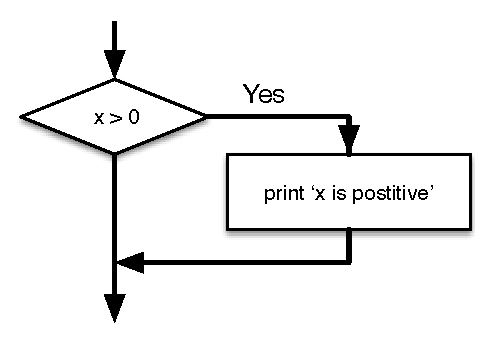
\includegraphics[keepaspectratio,alt={If Logic},height=1.5in]{../images/if.eps}}
\caption{If Logic}
\end{figure}

Kung ang logical condition ay true, pagkatapos ang indented statement ay
na-e-execute. Kung ang logical condition ay false, ang indented
statement ay na-skip.

\index{condition} \index{compound statement} \index{statement!compound}

Ang \texttt{if} statements ay may parehong structure sa function
definitions o \texttt{for} loops\footnote{Matututunan natin ang
  functions sa Chapter 4 at loops sa Chapter 5.}. Ang statement ay
binubuo ng header line na nagtatapos sa colon character (:) na
sinusundan ng indented block. Ang mga statements na ganito ay tinatawag
na \emph{compound statements} dahil umaabot sila sa higit sa isang
linya.

\begin{Shaded}
\begin{Highlighting}[]
\ControlFlowTok{if}\NormalTok{ x }\OperatorTok{\textgreater{}}\NormalTok{ y:}
    \BuiltInTok{print}\NormalTok{(x)}
    \BuiltInTok{print}\NormalTok{(y)}
\end{Highlighting}
\end{Shaded}

Walang limitasyon sa bilang ng statements na maaaring lumabas sa body,
pero dapat may hindi bababa sa isa. Paminsan-minsan, kapaki-pakinabang
na magkaroon ng body na walang statements (karaniwang bilang place
holder para sa code na hindi mo pa nasusulat). Sa kasong iyon, maaari
mong gamitin ang \texttt{pass} statement para makapasa sa Python
interpreter check, na walang ginagawa.

\index{pass statement} \index{statement!pass}

\begin{Shaded}
\begin{Highlighting}[]
\ControlFlowTok{if}\NormalTok{ x }\OperatorTok{\textless{}} \DecValTok{0}\NormalTok{ :}
    \ControlFlowTok{pass}   \CommentTok{\# need to handle negative values, do nothing for now.}
\end{Highlighting}
\end{Shaded}

Kung mag-e-enter ka ng \texttt{if} statement sa Python interpreter, ang
prompt ay magbabago mula sa tatlong chevrons
(\textgreater\textgreater\textgreater) patungo sa tatlong dots (\ldots)
para ipahiwatig na nasa gitna ka ng block ng statements, tulad ng
ipinakita sa ibaba:

\begin{Shaded}
\begin{Highlighting}[]
\OperatorTok{\textgreater{}\textgreater{}\textgreater{}}\NormalTok{ x }\OperatorTok{=} \DecValTok{3}
\OperatorTok{\textgreater{}\textgreater{}\textgreater{}} \ControlFlowTok{if}\NormalTok{ x }\OperatorTok{\textless{}} \DecValTok{10}\NormalTok{:}
\NormalTok{...    }\BuiltInTok{print}\NormalTok{(}\StringTok{\textquotesingle{}Small\textquotesingle{}}\NormalTok{)}
\NormalTok{...}
\NormalTok{Small}
\OperatorTok{\textgreater{}\textgreater{}\textgreater{}}
\end{Highlighting}
\end{Shaded}

Kapag gumagamit ng Python interpreter, kailangan mong mag-iwan ng blank
line sa dulo ng block, kung hindi ay magre-return ang Python ng error:

\begin{Shaded}
\begin{Highlighting}[]
\OperatorTok{\textgreater{}\textgreater{}\textgreater{}}\NormalTok{ x }\OperatorTok{=} \DecValTok{3}
\OperatorTok{\textgreater{}\textgreater{}\textgreater{}} \ControlFlowTok{if}\NormalTok{ x }\OperatorTok{\textless{}} \DecValTok{10}\NormalTok{:}
\NormalTok{...    }\BuiltInTok{print}\NormalTok{(}\StringTok{\textquotesingle{}Small\textquotesingle{}}\NormalTok{)}
\NormalTok{... }\BuiltInTok{print}\NormalTok{(}\StringTok{\textquotesingle{}Done\textquotesingle{}}\NormalTok{)}
\NormalTok{  File }\StringTok{"\textless{}stdin\textgreater{}"}\NormalTok{, line }\DecValTok{3}
    \BuiltInTok{print}\NormalTok{(}\StringTok{\textquotesingle{}Done\textquotesingle{}}\NormalTok{)}
        \OperatorTok{\^{}}
\PreprocessorTok{SyntaxError}\NormalTok{: invalid syntax}
\end{Highlighting}
\end{Shaded}

Ang blank line sa dulo ng block ng statements ay hindi kailangan kapag
sumusulat at nag-e-execute ng script, pero maaari itong mapabuti ang
readability ng iyong code.

\section{Alternative execution}\label{alternative-execution}

\index{alternative execution} \index{else keyword} \index{keyword!else}

Ang pangalawang form ng \texttt{if} statement ay \emph{alternative
execution}, kung saan mayroong dalawang posibilidad at ang condition ay
tumutukoy kung alin ang na-e-execute. Ang syntax ay ganito:

\begin{Shaded}
\begin{Highlighting}[]
\ControlFlowTok{if}\NormalTok{ x }\OperatorTok{\%} \DecValTok{2} \OperatorTok{==} \DecValTok{0}\NormalTok{:}
    \BuiltInTok{print}\NormalTok{(}\StringTok{\textquotesingle{}x is even\textquotesingle{}}\NormalTok{)}
\ControlFlowTok{else}\NormalTok{:}
    \BuiltInTok{print}\NormalTok{(}\StringTok{\textquotesingle{}x is odd\textquotesingle{}}\NormalTok{)}
\end{Highlighting}
\end{Shaded}

Kung ang remainder kapag ang \texttt{x} ay hinati sa 2 ay 0, pagkatapos
alam natin na ang \texttt{x} ay even, at ang program ay nagdi-display ng
mensahe tungkol dito. Kung ang condition ay false, ang pangalawang set
ng statements ay na-e-execute.

\begin{figure}
\centering
\pandocbounded{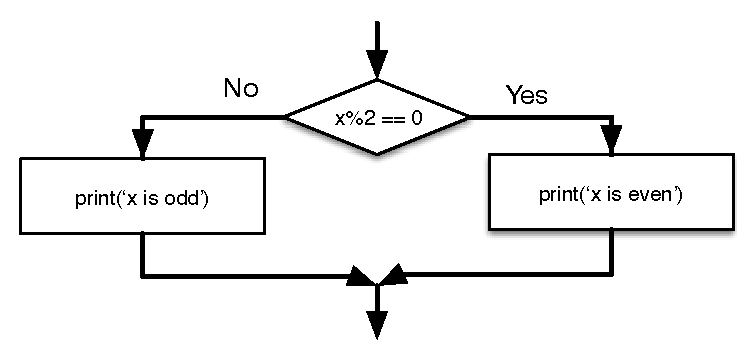
\includegraphics[keepaspectratio,alt={If-Then-Else Logic},height=1.5in]{../images/if-else.eps}}
\caption{If-Then-Else Logic}
\end{figure}

Dahil ang condition ay dapat na true o false, eksaktong isa sa mga
alternatives ang ma-e-execute. Ang mga alternatives ay tinatawag na
\emph{branches}, dahil sila ay branches sa flow ng execution.

\index{branch}

\section{Chained conditionals}\label{chained-conditionals}

\index{chained conditional} \index{conditional!chained}

Minsan mayroong higit sa dalawang posibilidad at kailangan natin ng
higit sa dalawang branches. Isang paraan para ipahayag ang computation
na ganito ay \emph{chained conditional}:

\begin{Shaded}
\begin{Highlighting}[]
\ControlFlowTok{if}\NormalTok{ x }\OperatorTok{\textless{}}\NormalTok{ y:}
    \BuiltInTok{print}\NormalTok{(}\StringTok{\textquotesingle{}x is less than y\textquotesingle{}}\NormalTok{)}
\ControlFlowTok{elif}\NormalTok{ x }\OperatorTok{\textgreater{}}\NormalTok{ y:}
    \BuiltInTok{print}\NormalTok{(}\StringTok{\textquotesingle{}x is greater than y\textquotesingle{}}\NormalTok{)}
\ControlFlowTok{else}\NormalTok{:}
    \BuiltInTok{print}\NormalTok{(}\StringTok{\textquotesingle{}x and y are equal\textquotesingle{}}\NormalTok{)}
\end{Highlighting}
\end{Shaded}

Ang \texttt{elif} ay abbreviation ng ``else if.'' Muli, eksaktong isang
branch ang ma-e-execute.

\begin{figure}
\centering
\pandocbounded{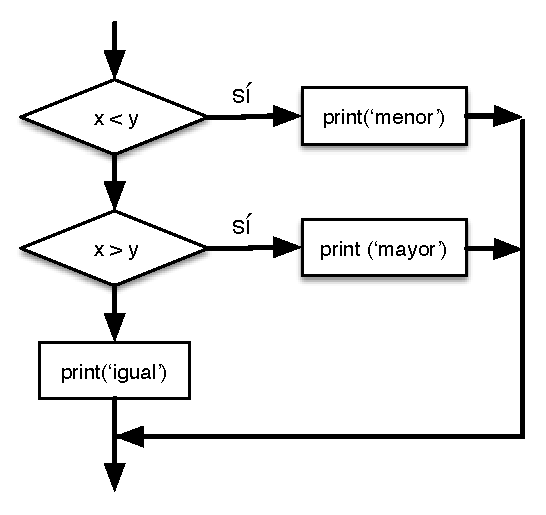
\includegraphics[keepaspectratio,alt={If-Then-ElseIf Logic},height=2.0in]{../images/elif.eps}}
\caption{If-Then-ElseIf Logic}
\end{figure}

Walang limitasyon sa bilang ng \texttt{elif} statements. Kung mayroong
\texttt{else} clause, dapat ito ay nasa dulo, pero hindi kailangan na
mayroon.

\index{elif keyword} \index{keyword!elif}

\begin{Shaded}
\begin{Highlighting}[]
\ControlFlowTok{if}\NormalTok{ choice }\OperatorTok{==} \StringTok{\textquotesingle{}a\textquotesingle{}}\NormalTok{:}
    \BuiltInTok{print}\NormalTok{(}\StringTok{\textquotesingle{}Bad guess\textquotesingle{}}\NormalTok{)}
\ControlFlowTok{elif}\NormalTok{ choice }\OperatorTok{==} \StringTok{\textquotesingle{}b\textquotesingle{}}\NormalTok{:}
    \BuiltInTok{print}\NormalTok{(}\StringTok{\textquotesingle{}Good guess\textquotesingle{}}\NormalTok{)}
\ControlFlowTok{elif}\NormalTok{ choice }\OperatorTok{==} \StringTok{\textquotesingle{}c\textquotesingle{}}\NormalTok{:}
    \BuiltInTok{print}\NormalTok{(}\StringTok{\textquotesingle{}Close, but not correct\textquotesingle{}}\NormalTok{)}
\end{Highlighting}
\end{Shaded}

Ang bawat condition ay sinusuri sa order. Kung ang una ay false, ang
susunod ay sinusuri, at iba pa. Kung ang isa sa kanila ay true, ang
corresponding branch ay na-e-execute, at ang statement ay nagtatapos.
Kahit na higit sa isang condition ay true, ang unang true branch lang
ang na-e-execute.

\section{Nested conditionals}\label{nested-conditionals}

\index{nested conditional} \index{conditional!nested}

Ang isang conditional ay maaari ring i-nest sa loob ng isa pa. Maaari
nating isulat ang three-branch example na ganito:

\begin{Shaded}
\begin{Highlighting}[]
\ControlFlowTok{if}\NormalTok{ x }\OperatorTok{==}\NormalTok{ y:}
    \BuiltInTok{print}\NormalTok{(}\StringTok{\textquotesingle{}x and y are equal\textquotesingle{}}\NormalTok{)}
\ControlFlowTok{else}\NormalTok{:}
    \ControlFlowTok{if}\NormalTok{ x }\OperatorTok{\textless{}}\NormalTok{ y:}
        \BuiltInTok{print}\NormalTok{(}\StringTok{\textquotesingle{}x is less than y\textquotesingle{}}\NormalTok{)}
    \ControlFlowTok{else}\NormalTok{:}
        \BuiltInTok{print}\NormalTok{(}\StringTok{\textquotesingle{}x is greater than y\textquotesingle{}}\NormalTok{)}
\end{Highlighting}
\end{Shaded}

Ang outer conditional ay naglalaman ng dalawang branches. Ang unang
branch ay naglalaman ng simpleng statement. Ang pangalawang branch ay
naglalaman ng iba pang \texttt{if} statement, na may dalawang branches
din. Ang dalawang branches na iyon ay parehong simpleng statements,
bagaman maaari silang maging conditional statements din.

\begin{figure}
\centering
\pandocbounded{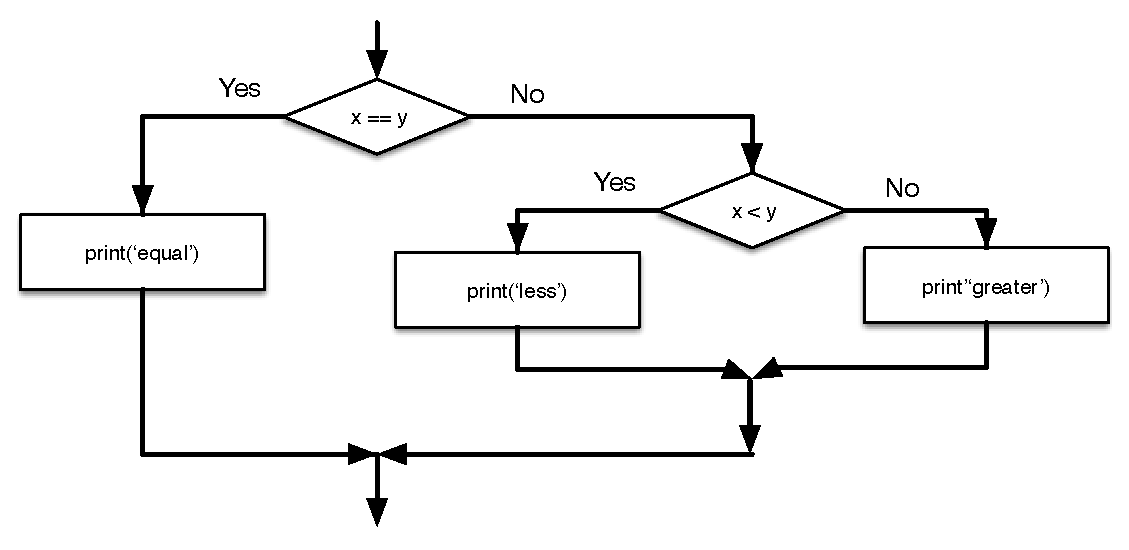
\includegraphics[keepaspectratio,alt={Nested If Statements},height=2.0in]{../images/nested.eps}}
\caption{Nested If Statements}
\end{figure}

Bagaman ang indentation ng statements ay ginagawang halata ang
structure, ang \emph{nested conditionals} ay nagiging mahirap basahin
nang napakabilis. Sa pangkalahatan, magandang ideya na iwasan ang mga
ito kapag maaari.

Ang logical operators ay kadalasang nagbibigay ng paraan para gawing
simple ang nested conditional statements. Halimbawa, maaari nating
muling isulat ang sumusunod na code gamit ang isang conditional:

\begin{Shaded}
\begin{Highlighting}[]
\ControlFlowTok{if} \DecValTok{0} \OperatorTok{\textless{}}\NormalTok{ x:}
    \ControlFlowTok{if}\NormalTok{ x }\OperatorTok{\textless{}} \DecValTok{10}\NormalTok{:}
        \BuiltInTok{print}\NormalTok{(}\StringTok{\textquotesingle{}x is a positive single{-}digit number.\textquotesingle{}}\NormalTok{)}
\end{Highlighting}
\end{Shaded}

Ang \texttt{print} statement ay na-e-execute lang kapag pumasa tayo sa
parehong conditionals. Maaari nating makuha ang parehong epekto gamit
ang \texttt{and} operator:

\begin{Shaded}
\begin{Highlighting}[]
\ControlFlowTok{if} \DecValTok{0} \OperatorTok{\textless{}}\NormalTok{ x }\KeywordTok{and}\NormalTok{ x }\OperatorTok{\textless{}} \DecValTok{10}\NormalTok{:}
    \BuiltInTok{print}\NormalTok{(}\StringTok{\textquotesingle{}x is a positive single{-}digit number.\textquotesingle{}}\NormalTok{)}
\end{Highlighting}
\end{Shaded}

\section{Catching exceptions using try and
except}\label{catching-exceptions-using-try-and-except}

Mas maaga nakita natin ang code segment kung saan ginamit natin ang
\texttt{input} at \texttt{int} functions para basahin at i-parse ang
integer number na na-enter ng user. Nakita din natin kung gaano
kadelikado ang paggawa nito:

\begin{Shaded}
\begin{Highlighting}[]
\OperatorTok{\textgreater{}\textgreater{}\textgreater{}}\NormalTok{ prompt }\OperatorTok{=} \StringTok{"What is the air velocity of an unladen swallow?}\CharTok{\textbackslash{}n}\StringTok{"}
\OperatorTok{\textgreater{}\textgreater{}\textgreater{}}\NormalTok{ speed }\OperatorTok{=} \BuiltInTok{input}\NormalTok{(prompt)}
\NormalTok{What }\KeywordTok{is}\NormalTok{ the air velocity of an unladen swallow?}
\NormalTok{What do you mean, an African }\KeywordTok{or}\NormalTok{ a European swallow?}
\OperatorTok{\textgreater{}\textgreater{}\textgreater{}} \BuiltInTok{int}\NormalTok{(speed)}
\PreprocessorTok{ValueError}\NormalTok{: invalid literal }\ControlFlowTok{for} \BuiltInTok{int}\NormalTok{() }\ControlFlowTok{with}
\NormalTok{base }\DecValTok{10}\NormalTok{: }\StringTok{\textquotesingle{}What do you mean, an African or a European swallow?\textquotesingle{}}
\OperatorTok{\textgreater{}\textgreater{}\textgreater{}}
\end{Highlighting}
\end{Shaded}

Kapag nag-e-execute tayo ng mga statements na ito sa Python interpreter,
nakakakuha tayo ng bagong prompt mula sa interpreter, iniisip natin ang
``oops'', at nagpapatuloy sa susunod nating statement.

Gayunpaman kung ilalagay mo ang code na ito sa Python script at mangyari
ang error na ito, ang iyong script ay agad na humihinto sa track nito na
may traceback. Hindi ito nag-e-execute ng sumusunod na statement.

\index{traceback}

Narito ang sample program para i-convert ang Fahrenheit temperature sa
Celsius temperature:

\index{fahrenheit} \index{celsius} \index{temperature conversion}

\begin{Shaded}
\begin{Highlighting}[]
\NormalTok{inp }\OperatorTok{=} \BuiltInTok{input}\NormalTok{(}\StringTok{\textquotesingle{}Enter Fahrenheit Temperature: \textquotesingle{}}\NormalTok{)}
\NormalTok{fahr }\OperatorTok{=} \BuiltInTok{float}\NormalTok{(inp)}
\NormalTok{cel }\OperatorTok{=}\NormalTok{ (fahr }\OperatorTok{{-}} \FloatTok{32.0}\NormalTok{) }\OperatorTok{*} \FloatTok{5.0} \OperatorTok{/} \FloatTok{9.0}
\BuiltInTok{print}\NormalTok{(cel)}

\CommentTok{\# Code: https://www.py4e.com/code3/fahren.py}
\end{Highlighting}
\end{Shaded}

Kung i-e-execute natin ang code na ito at bigyan ito ng invalid input,
simpleng nabibigo ito na may unfriendly error message:

{\small
\begin{verbatim}
python fahren.py
Enter Fahrenheit Temperature:72
22.22222222222222
\end{verbatim}
}

{\small
\begin{verbatim}
python fahren.py
Enter Fahrenheit Temperature:fred
Traceback (most recent call last):
  File "fahren.py", line 2, in <module>
    fahr = float(inp)
ValueError: could not convert string to float: 'fred'
\end{verbatim}
}

Mayroong conditional execution structure na built-in sa Python para
haharapin ang mga uri ng expected at unexpected errors na tinatawag na
``try / except''. Ang layunin ng \texttt{try} at \texttt{except} ay alam
mo na ang ilang sequence ng instruction(s) ay maaaring may problema at
gusto mong magdagdag ng ilang statements para i-execute kung may error
na mangyari. Ang mga extra statements na ito (ang except block) ay hindi
pinapansin kung walang error.

Maaari mong isipin ang \texttt{try} at \texttt{except} feature sa Python
bilang ``insurance policy'' sa sequence ng statements.

Maaari nating muling isulat ang temperature converter natin tulad ng
sumusunod:

\begin{Shaded}
\begin{Highlighting}[]
\NormalTok{inp }\OperatorTok{=} \BuiltInTok{input}\NormalTok{(}\StringTok{\textquotesingle{}Enter Fahrenheit Temperature:\textquotesingle{}}\NormalTok{)}
\ControlFlowTok{try}\NormalTok{:}
\NormalTok{    fahr }\OperatorTok{=} \BuiltInTok{float}\NormalTok{(inp)}
\NormalTok{    cel }\OperatorTok{=}\NormalTok{ (fahr }\OperatorTok{{-}} \FloatTok{32.0}\NormalTok{) }\OperatorTok{*} \FloatTok{5.0} \OperatorTok{/} \FloatTok{9.0}
    \BuiltInTok{print}\NormalTok{(cel)}
\ControlFlowTok{except}\NormalTok{:}
    \BuiltInTok{print}\NormalTok{(}\StringTok{\textquotesingle{}Please enter a number\textquotesingle{}}\NormalTok{)}

\CommentTok{\# Code: https://www.py4e.com/code3/fahren2.py}
\end{Highlighting}
\end{Shaded}

Ang Python ay nagsisimula sa pag-e-execute ng sequence ng statements sa
\texttt{try} block. Kung maayos ang lahat, i-skip nito ang
\texttt{except} block at magpapatuloy. Kung may exception na mangyari sa
\texttt{try} block, ang Python ay lumalabas sa \texttt{try} block at
nag-e-execute ng sequence ng statements sa \texttt{except} block.

{\small
\begin{verbatim}
python fahren2.py
Enter Fahrenheit Temperature:72
22.22222222222222
\end{verbatim}
}

{\small
\begin{verbatim}
python fahren2.py
Enter Fahrenheit Temperature:fred
Please enter a number
\end{verbatim}
}

Ang pagharap sa exception gamit ang \texttt{try} statement ay tinatawag
na \emph{catching} ng exception. Sa halimbawang ito, ang \texttt{except}
clause ay nagpi-print ng error message. Sa pangkalahatan, ang pag-catch
ng exception ay nagbibigay sa iyo ng pagkakataon na ayusin ang problema,
o subukan ulit, o hindi bababa ay tapusin ang program nang maayos.

\section{Short-circuit evaluation of logical
expressions}\label{short-circuit-evaluation-of-logical-expressions}

\index{short circuit}

Kapag nagpo-process ang Python ng logical expression tulad ng
\texttt{x\ \textgreater{}=\ 2\ and\ (x/y)\ \textgreater{}\ 2},
i-e-evaluate nito ang expression mula kaliwa hanggang kanan. Dahil sa
definition ng \texttt{and}, kung ang \texttt{x} ay mas maliit sa 2, ang
expression na \texttt{x\ \textgreater{}=\ 2} ay \texttt{False} at kaya
ang buong expression ay \texttt{False} anuman kung ang
\texttt{(x/y)\ \textgreater{}\ 2} ay nag-e-evaluate sa \texttt{True} o
\texttt{False}.

Kapag nakita ng Python na walang makukuha sa pag-e-evaluate ng
natitirang bahagi ng logical expression, humihinto ito sa evaluation at
hindi ginagawa ang computations sa natitirang bahagi ng logical
expression. Kapag ang evaluation ng logical expression ay humihinto
dahil ang overall value ay alam na, ito ay tinatawag na
\emph{short-circuiting} ang evaluation.

\index{guardian pattern} \index{pattern!guardian}

Habang ito ay maaaring mukhang fine point, ang short-circuit behavior ay
nagdudulot sa matalinong technique na tinatawag na \emph{guardian
pattern}. Isaalang-alang ang sumusunod na code sequence sa Python
interpreter:

\begin{Shaded}
\begin{Highlighting}[]
\OperatorTok{\textgreater{}\textgreater{}\textgreater{}}\NormalTok{ x }\OperatorTok{=} \DecValTok{6}
\OperatorTok{\textgreater{}\textgreater{}\textgreater{}}\NormalTok{ y }\OperatorTok{=} \DecValTok{2}
\OperatorTok{\textgreater{}\textgreater{}\textgreater{}}\NormalTok{ x }\OperatorTok{\textgreater{}=} \DecValTok{2} \KeywordTok{and}\NormalTok{ (x}\OperatorTok{/}\NormalTok{y) }\OperatorTok{\textgreater{}} \DecValTok{2}
\VariableTok{True}
\OperatorTok{\textgreater{}\textgreater{}\textgreater{}}\NormalTok{ x }\OperatorTok{=} \DecValTok{1}
\OperatorTok{\textgreater{}\textgreater{}\textgreater{}}\NormalTok{ y }\OperatorTok{=} \DecValTok{0}
\OperatorTok{\textgreater{}\textgreater{}\textgreater{}}\NormalTok{ x }\OperatorTok{\textgreater{}=} \DecValTok{2} \KeywordTok{and}\NormalTok{ (x}\OperatorTok{/}\NormalTok{y) }\OperatorTok{\textgreater{}} \DecValTok{2}
\VariableTok{False}
\OperatorTok{\textgreater{}\textgreater{}\textgreater{}}\NormalTok{ x }\OperatorTok{=} \DecValTok{6}
\OperatorTok{\textgreater{}\textgreater{}\textgreater{}}\NormalTok{ y }\OperatorTok{=} \DecValTok{0}
\OperatorTok{\textgreater{}\textgreater{}\textgreater{}}\NormalTok{ x }\OperatorTok{\textgreater{}=} \DecValTok{2} \KeywordTok{and}\NormalTok{ (x}\OperatorTok{/}\NormalTok{y) }\OperatorTok{\textgreater{}} \DecValTok{2}
\NormalTok{Traceback (most recent call last):}
\NormalTok{  File }\StringTok{"\textless{}stdin\textgreater{}"}\NormalTok{, line }\DecValTok{1}\NormalTok{, }\KeywordTok{in} \OperatorTok{\textless{}}\NormalTok{module}\OperatorTok{\textgreater{}}
\PreprocessorTok{ZeroDivisionError}\NormalTok{: division by zero}
\OperatorTok{\textgreater{}\textgreater{}\textgreater{}}
\end{Highlighting}
\end{Shaded}

Ang pangatlong calculation ay nabigo dahil ang Python ay nag-e-evaluate
ng \texttt{(x/y)} at ang \texttt{y} ay zero, na nagdudulot ng runtime
error. Pero ang una at pangalawang halimbawa ay \emph{hindi} nabigo
dahil sa unang calculation ang \texttt{y} ay non zero at sa pangalawa
ang unang parte ng mga expressions na ito na
\texttt{x\ \textgreater{}=\ 2} ay nag-e-evaluate sa \texttt{False} kaya
ang \texttt{(x/y)} ay hindi kailanman na-e-execute dahil sa
\emph{short-circuit} rule at walang error.

Maaari nating gawin ang logical expression para strategically maglagay
ng \emph{guard} evaluation bago lang ang evaluation na maaaring magdulot
ng error tulad ng sumusunod:

\begin{Shaded}
\begin{Highlighting}[]
\OperatorTok{\textgreater{}\textgreater{}\textgreater{}}\NormalTok{ x }\OperatorTok{=} \DecValTok{1}
\OperatorTok{\textgreater{}\textgreater{}\textgreater{}}\NormalTok{ y }\OperatorTok{=} \DecValTok{0}
\OperatorTok{\textgreater{}\textgreater{}\textgreater{}}\NormalTok{ x }\OperatorTok{\textgreater{}=} \DecValTok{2} \KeywordTok{and}\NormalTok{ y }\OperatorTok{!=} \DecValTok{0} \KeywordTok{and}\NormalTok{ (x}\OperatorTok{/}\NormalTok{y) }\OperatorTok{\textgreater{}} \DecValTok{2}
\VariableTok{False}
\OperatorTok{\textgreater{}\textgreater{}\textgreater{}}\NormalTok{ x }\OperatorTok{=} \DecValTok{6}
\OperatorTok{\textgreater{}\textgreater{}\textgreater{}}\NormalTok{ y }\OperatorTok{=} \DecValTok{0}
\OperatorTok{\textgreater{}\textgreater{}\textgreater{}}\NormalTok{ x }\OperatorTok{\textgreater{}=} \DecValTok{2} \KeywordTok{and}\NormalTok{ y }\OperatorTok{!=} \DecValTok{0} \KeywordTok{and}\NormalTok{ (x}\OperatorTok{/}\NormalTok{y) }\OperatorTok{\textgreater{}} \DecValTok{2}
\VariableTok{False}
\OperatorTok{\textgreater{}\textgreater{}\textgreater{}}\NormalTok{ x }\OperatorTok{\textgreater{}=} \DecValTok{2} \KeywordTok{and}\NormalTok{ (x}\OperatorTok{/}\NormalTok{y) }\OperatorTok{\textgreater{}} \DecValTok{2} \KeywordTok{and}\NormalTok{ y }\OperatorTok{!=} \DecValTok{0}
\NormalTok{Traceback (most recent call last):}
\NormalTok{  File }\StringTok{"\textless{}stdin\textgreater{}"}\NormalTok{, line }\DecValTok{1}\NormalTok{, }\KeywordTok{in} \OperatorTok{\textless{}}\NormalTok{module}\OperatorTok{\textgreater{}}
\PreprocessorTok{ZeroDivisionError}\NormalTok{: division by zero}
\OperatorTok{\textgreater{}\textgreater{}\textgreater{}}
\end{Highlighting}
\end{Shaded}

Sa unang logical expression, ang \texttt{x\ \textgreater{}=\ 2} ay
\texttt{False} kaya ang evaluation ay humihinto sa \texttt{and}. Sa
pangalawang logical expression, ang \texttt{x\ \textgreater{}=\ 2} ay
\texttt{True} pero ang \texttt{y\ !=\ 0} ay \texttt{False} kaya hindi
natin naabot ang \texttt{(x/y)}.

Sa pangatlong logical expression, ang \texttt{y\ !=\ 0} ay
\emph{pagkatapos} ng \texttt{(x/y)} calculation kaya ang expression ay
nabibigo na may error.

Sa pangalawang expression, sinasabi natin na ang \texttt{y\ !=\ 0} ay
nagsisilbing \emph{guard} para masiguro na i-e-execute lang natin ang
\texttt{(x/y)} kung ang \texttt{y} ay non-zero.

\section{Debugging}\label{debugging-2}

\index{debugging} \index{traceback}

Ang traceback na ipinapakita ng Python kapag may error ay naglalaman ng
maraming information, pero maaari itong maging overwhelming. Ang
pinakakapaki-pakinabang na parts ay karaniwang:

\begin{itemize}
\item
  Anong uri ng error ito, at
\item
  Saan ito nangyari.
\end{itemize}

Ang syntax errors ay karaniwang madaling hanapin, pero may ilang
gotchas. Ang whitespace errors ay maaaring nakakalito dahil ang spaces
at tabs ay invisible at sanay tayong hindi pinapansin ang mga ito.

\index{whitespace}

\begin{Shaded}
\begin{Highlighting}[]
\OperatorTok{\textgreater{}\textgreater{}\textgreater{}}\NormalTok{ x }\OperatorTok{=} \DecValTok{5}
\OperatorTok{\textgreater{}\textgreater{}\textgreater{}}\NormalTok{  y }\OperatorTok{=} \DecValTok{6}
\NormalTok{  File }\StringTok{"\textless{}stdin\textgreater{}"}\NormalTok{, line }\DecValTok{1}
\NormalTok{    y }\OperatorTok{=} \DecValTok{6}
    \OperatorTok{\^{}}
\PreprocessorTok{IndentationError}\NormalTok{: unexpected indent}
\end{Highlighting}
\end{Shaded}

Sa halimbawang ito, ang problema ay ang pangalawang linya ay naka-indent
ng isang space. Pero ang error message ay tumuturo sa \texttt{y}, na
nakakalito. Sa pangkalahatan, ang error messages ay nagpapahiwatig kung
saan natuklasan ang problema, pero ang actual error ay maaaring mas
maaga sa code, minsan sa naunang linya.

Sa pangkalahatan, ang error messages ay nagsasabi sa iyo kung saan
natuklasan ang problema, pero iyon ay kadalasang hindi kung saan ito
naging sanhi.

\section{Glossary}\label{glossary-2}

\begin{description}
\tightlist
\item[body]
Ang sequence ng statements sa loob ng compound statement. \index{body}
\item[boolean expression]
Expression na ang value ay maaaring \texttt{True} o \texttt{False}.
\index{boolean expression} \index{expression!boolean}
\item[branch]
Isa sa mga alternative sequences ng statements sa conditional statement.
\index{branch}
\item[chained conditional]
Conditional statement na may serye ng alternative branches.
\index{chained conditional} \index{conditional!chained}
\item[comparison operator]
Isa sa mga operators na nagko-compare ng mga operands nito: \texttt{==},
\texttt{!=}, \texttt{\textgreater{}}, \texttt{\textless{}},
\texttt{\textgreater{}=}, at \texttt{\textless{}=}.
\item[conditional statement]
Statement na kumokontrol sa flow ng execution depende sa ilang
condition. \index{conditional statement} \index{statement!conditional}
\item[condition]
Ang boolean expression sa conditional statement na tumutukoy kung aling
branch ang na-e-execute. \index{condition}
\item[compound statement]
Statement na binubuo ng header at body. Ang header ay nagtatapos sa
colon (:). Ang body ay naka-indent relative sa header.
\index{compound statement}
\item[guardian pattern]
Kung saan gumagawa tayo ng logical expression na may additional
comparisons para samantalahin ang short-circuit behavior.
\index{guardian pattern} \index{pattern!guardian}
\item[logical operator]
Isa sa mga operators na nagko-combine ng boolean expressions:
\texttt{and}, \texttt{or}, at \texttt{not}.
\item[nested conditional]
Conditional statement na lumalabas sa isa sa mga branches ng iba pang
conditional statement. \index{nested conditional}
\index{conditional!nested}
\item[traceback]
List ng mga functions na nag-e-execute, na na-print kapag may exception
na nangyari. \index{traceback}
\item[short circuit]
Kapag ang Python ay nasa gitna ng pag-e-evaluate ng logical expression
at humihinto sa evaluation dahil alam na ng Python ang final value para
sa expression nang hindi kailangan i-evaluate ang natitirang bahagi ng
expression. \index{short circuit}
\end{description}

\section{Exercises}\label{exercises-2}

\textbf{Exercise 1:} Muling isulat ang iyong pay computation para bigyan
ang employee ng 1.5 beses ang hourly rate para sa hours na nagtrabaho sa
itaas ng 40 hours.

{\small
\begin{verbatim}
Enter Hours: 45
Enter Rate: 10
Pay: 475.0
\end{verbatim}
}

\textbf{Exercise 2:} Muling isulat ang iyong pay program gamit ang
\texttt{try} at \texttt{except} para ang iyong program ay haharapin ang
non-numeric input nang maayos sa pamamagitan ng pag-print ng mensahe at
pag-exit sa program. Ang sumusunod ay nagpapakita ng dalawang executions
ng program:

{\small
\begin{verbatim}
Enter Hours: 20
Enter Rate: nine
Error, please enter numeric input
\end{verbatim}
}

{\small
\begin{verbatim}
Enter Hours: forty
Error, please enter numeric input
\end{verbatim}
}

\textbf{Exercise 3:} Sumulat ng program para mag-prompt para sa score sa
pagitan ng 0.0 at 1.0. Kung ang score ay nasa labas ng range, mag-print
ng error message. Kung ang score ay sa pagitan ng 0.0 at 1.0, mag-print
ng grade gamit ang sumusunod na table:

{\small
\begin{verbatim}
 Score   Grade
>= 0.9     A
>= 0.8     B
>= 0.7     C
>= 0.6     D
 < 0.6     F
\end{verbatim}
}

{\small
\begin{verbatim}
Enter score: 0.95
A
\end{verbatim}
}

{\small
\begin{verbatim}
Enter score: perfect
Bad score
\end{verbatim}
}

{\small
\begin{verbatim}
Enter score: 10.0
Bad score
\end{verbatim}
}

{\small
\begin{verbatim}
Enter score: 0.75
C
\end{verbatim}
}

{\small
\begin{verbatim}
Enter score: 0.5
F
\end{verbatim}
}

Patakbuhin ang program nang paulit-ulit tulad ng ipinakita sa itaas para
i-test ang iba't ibang values para sa input.

\chapter{Functions}\label{functions}

\section{Function calls}\label{function-calls}

\index{function call}

Sa konteksto ng programming, ang \emph{function} ay pinangalanang
sequence ng statements na gumagawa ng computation. Kapag nagde-define ka
ng function, tinutukoy mo ang pangalan at ang sequence ng statements.
Mamaya, maaari mong ``tawagin'' ang function sa pamamagitan ng pangalan.
Nakita na natin ang isang halimbawa ng \emph{function call}:

\begin{Shaded}
\begin{Highlighting}[]
\OperatorTok{\textgreater{}\textgreater{}\textgreater{}} \BuiltInTok{type}\NormalTok{(}\DecValTok{32}\NormalTok{)}
\OperatorTok{\textless{}}\KeywordTok{class} \StringTok{\textquotesingle{}int\textquotesingle{}}\OperatorTok{\textgreater{}}
\end{Highlighting}
\end{Shaded}

Ang pangalan ng function ay \texttt{type}. Ang expression sa parentheses
ay tinatawag na \emph{argument} ng function. Ang argument ay value o
variable na ipinapasa natin sa function bilang input sa function. Ang
result, para sa \texttt{type} function, ay ang type ng argument.

\index{parentheses!argument in}

Karaniwang sinasabi na ang function ay ``tumatanggap'' ng argument at
``nagre-return'' ng result. Ang result ay tinatawag na \emph{return
value}.

\index{argument} \index{return value}

\section{Built-in functions}\label{built-in-functions}

Ang Python ay nagbibigay ng maraming important built-in functions na
maaari nating gamitin nang hindi kailangan magbigay ng function
definition. Ang mga creators ng Python ay sumulat ng set ng functions
para solusyonan ang common problems at isinama sila sa Python para sa
atin na gamitin.

Ang \texttt{max} at \texttt{min} functions ay nagbibigay sa atin ng
pinakamalaki at pinakamaliit na values sa list, ayon sa pagkakabanggit:

\begin{Shaded}
\begin{Highlighting}[]
\OperatorTok{\textgreater{}\textgreater{}\textgreater{}} \BuiltInTok{max}\NormalTok{(}\StringTok{\textquotesingle{}Hello world\textquotesingle{}}\NormalTok{)}
\CommentTok{\textquotesingle{}w\textquotesingle{}}
\OperatorTok{\textgreater{}\textgreater{}\textgreater{}} \BuiltInTok{min}\NormalTok{(}\StringTok{\textquotesingle{}Hello world\textquotesingle{}}\NormalTok{)}
\CommentTok{\textquotesingle{} \textquotesingle{}}
\OperatorTok{\textgreater{}\textgreater{}\textgreater{}}
\end{Highlighting}
\end{Shaded}

Ang \texttt{max} function ay nagsasabi sa atin ng ``largest character''
sa string (na lumalabas na letrang ``w'') at ang \texttt{min} function
ay nagpapakita sa atin ng smallest character (na lumalabas na space).

Ang isa pang napakakaraniwang built-in function ay ang \texttt{len}
function na nagsasabi sa atin kung ilang items ang nasa argument nito.
Kung ang argument sa \texttt{len} ay string, nagre-return ito ng bilang
ng characters sa string.

\begin{Shaded}
\begin{Highlighting}[]
\OperatorTok{\textgreater{}\textgreater{}\textgreater{}} \BuiltInTok{len}\NormalTok{(}\StringTok{\textquotesingle{}Hello world\textquotesingle{}}\NormalTok{)}
\DecValTok{11}
\OperatorTok{\textgreater{}\textgreater{}\textgreater{}}
\end{Highlighting}
\end{Shaded}

Ang mga functions na ito ay hindi limitado sa pagtingin sa strings.
Maaari silang gumana sa anumang set ng values, tulad ng makikita natin
sa susunod na chapters.

Dapat mong ituring ang mga pangalan ng built-in functions bilang
reserved words (i.e., iwasan ang paggamit ng ``max'' bilang variable
name).

\section{Type conversion functions}\label{type-conversion-functions}

\index{conversion!type} \index{type conversion}

Ang Python ay nagbibigay din ng built-in functions na nagko-convert ng
values mula sa isang type patungo sa iba. Ang \texttt{int} function ay
tumatanggap ng anumang value at nagko-convert nito sa integer, kung
kaya, o nagre-reklamo kung hindi:

\index{int function} \index{function!int}

\begin{Shaded}
\begin{Highlighting}[]
\OperatorTok{\textgreater{}\textgreater{}\textgreater{}} \BuiltInTok{int}\NormalTok{(}\StringTok{\textquotesingle{}32\textquotesingle{}}\NormalTok{)}
\DecValTok{32}
\OperatorTok{\textgreater{}\textgreater{}\textgreater{}} \BuiltInTok{int}\NormalTok{(}\StringTok{\textquotesingle{}Hello\textquotesingle{}}\NormalTok{)}
\PreprocessorTok{ValueError}\NormalTok{: invalid literal }\ControlFlowTok{for} \BuiltInTok{int}\NormalTok{() }\ControlFlowTok{with}\NormalTok{ base }\DecValTok{10}\NormalTok{: }\StringTok{\textquotesingle{}Hello\textquotesingle{}}
\end{Highlighting}
\end{Shaded}

Ang \texttt{int} ay maaaring mag-convert ng floating-point values sa
integers, pero hindi ito nagro-round off; tinatanggal nito ang fraction
part:

\begin{Shaded}
\begin{Highlighting}[]
\OperatorTok{\textgreater{}\textgreater{}\textgreater{}} \BuiltInTok{int}\NormalTok{(}\FloatTok{3.99999}\NormalTok{)}
\DecValTok{3}
\OperatorTok{\textgreater{}\textgreater{}\textgreater{}} \BuiltInTok{int}\NormalTok{(}\OperatorTok{{-}}\FloatTok{2.3}\NormalTok{)}
\OperatorTok{{-}}\DecValTok{2}
\end{Highlighting}
\end{Shaded}

Ang \texttt{float} ay nagko-convert ng integers at strings sa
floating-point numbers:

\index{float function} \index{function!float}

\begin{Shaded}
\begin{Highlighting}[]
\OperatorTok{\textgreater{}\textgreater{}\textgreater{}} \BuiltInTok{float}\NormalTok{(}\DecValTok{32}\NormalTok{)}
\FloatTok{32.0}
\OperatorTok{\textgreater{}\textgreater{}\textgreater{}} \BuiltInTok{float}\NormalTok{(}\StringTok{\textquotesingle{}3.14159\textquotesingle{}}\NormalTok{)}
\FloatTok{3.14159}
\end{Highlighting}
\end{Shaded}

Sa wakas, ang \texttt{str} ay nagko-convert ng argument nito sa string:

\index{str function} \index{function!str}

\begin{Shaded}
\begin{Highlighting}[]
\OperatorTok{\textgreater{}\textgreater{}\textgreater{}} \BuiltInTok{str}\NormalTok{(}\DecValTok{32}\NormalTok{)}
\CommentTok{\textquotesingle{}32\textquotesingle{}}
\OperatorTok{\textgreater{}\textgreater{}\textgreater{}} \BuiltInTok{str}\NormalTok{(}\FloatTok{3.14159}\NormalTok{)}
\CommentTok{\textquotesingle{}3.14159\textquotesingle{}}
\end{Highlighting}
\end{Shaded}

\section{Math functions}\label{math-functions}

\index{math function} \index{function, math} \index{module}
\index{module object}

Ang Python ay may \texttt{math} module na nagbibigay ng karamihan sa
pamilyar na mathematical functions. Bago natin magamit ang module,
kailangan nating i-import ito:

\begin{Shaded}
\begin{Highlighting}[]
\OperatorTok{\textgreater{}\textgreater{}\textgreater{}} \ImportTok{import}\NormalTok{ math}
\end{Highlighting}
\end{Shaded}

Ang statement na ito ay gumagawa ng \emph{module object} na may
pangalang math. Kung i-print mo ang module object, makakakuha ka ng
ilang information tungkol dito:

\begin{Shaded}
\begin{Highlighting}[]
\OperatorTok{\textgreater{}\textgreater{}\textgreater{}} \BuiltInTok{print}\NormalTok{(math)}
\OperatorTok{\textless{}}\NormalTok{module }\StringTok{\textquotesingle{}math\textquotesingle{}}\NormalTok{ (built}\OperatorTok{{-}}\KeywordTok{in}\NormalTok{)}\OperatorTok{\textgreater{}}
\end{Highlighting}
\end{Shaded}

Ang module object ay naglalaman ng mga functions at variables na tinukoy
sa module. Para ma-access ang isa sa mga functions, kailangan mong
tukuyin ang pangalan ng module at ang pangalan ng function, na
pinaghihiwalay ng dot (kilala din bilang period). Ang format na ito ay
tinatawag na \emph{dot notation}.

\index{dot notation}

\begin{Shaded}
\begin{Highlighting}[]
\OperatorTok{\textgreater{}\textgreater{}\textgreater{}}\NormalTok{ ratio }\OperatorTok{=}\NormalTok{ signal\_power }\OperatorTok{/}\NormalTok{ noise\_power}
\OperatorTok{\textgreater{}\textgreater{}\textgreater{}}\NormalTok{ decibels }\OperatorTok{=} \DecValTok{10} \OperatorTok{*}\NormalTok{ math.log10(ratio)}

\OperatorTok{\textgreater{}\textgreater{}\textgreater{}}\NormalTok{ radians }\OperatorTok{=} \FloatTok{0.7}
\OperatorTok{\textgreater{}\textgreater{}\textgreater{}}\NormalTok{ height }\OperatorTok{=}\NormalTok{ math.sin(radians)}
\end{Highlighting}
\end{Shaded}

Ang unang halimbawa ay nagko-compute ng logarithm base 10 ng
signal-to-noise ratio. Ang math module ay nagbibigay din ng function na
tinatawag na \texttt{log} na nagko-compute ng logarithms base e.

\index{log function} \index{function!log} \index{sine function}
\index{radian} \index{trigonometric function}
\index{function, trigonometric}

Ang pangalawang halimbawa ay nakakahanap ng sine ng \texttt{radians}.
Ang pangalan ng variable ay hint na ang \texttt{sin} at ang iba pang
trigonometric functions (\texttt{cos}, \texttt{tan}, etc.) ay
tumatanggap ng arguments sa radians. Para i-convert mula sa degrees
patungo sa radians, hatiin sa 360 at i-multiply sa \(2
\pi\):

\begin{Shaded}
\begin{Highlighting}[]
\OperatorTok{\textgreater{}\textgreater{}\textgreater{}}\NormalTok{ degrees }\OperatorTok{=} \DecValTok{45}
\OperatorTok{\textgreater{}\textgreater{}\textgreater{}}\NormalTok{ radians }\OperatorTok{=}\NormalTok{ degrees }\OperatorTok{/} \FloatTok{360.0} \OperatorTok{*} \DecValTok{2} \OperatorTok{*}\NormalTok{ math.pi}
\OperatorTok{\textgreater{}\textgreater{}\textgreater{}}\NormalTok{ math.sin(radians)}
\FloatTok{0.7071067811865476}
\end{Highlighting}
\end{Shaded}

Ang expression na \texttt{math.pi} ay kumukuha ng variable na
\texttt{pi} mula sa math module. Ang value ng variable na ito ay
approximation ng \(\pi\), tumpak sa humigit-kumulang 15 digits.

\index{pi}

Kung alam mo ang trigonometry mo, maaari mong suriin ang naunang result
sa pamamagitan ng pag-compare nito sa square root ng dalawa na hinati sa
dalawa:

\index{sqrt function} \index{function!sqrt}

\begin{Shaded}
\begin{Highlighting}[]
\OperatorTok{\textgreater{}\textgreater{}\textgreater{}}\NormalTok{ math.sqrt(}\DecValTok{2}\NormalTok{) }\OperatorTok{/} \FloatTok{2.0}
\FloatTok{0.7071067811865476}
\end{Highlighting}
\end{Shaded}

\section{Random numbers}\label{random-numbers}

\index{random number} \index{number, random} \index{deterministic}
\index{pseudorandom}

Sa parehong inputs, karamihan ng computer programs ay gumagawa ng
parehong outputs sa bawat pagkakataon, kaya sinasabi na sila ay
\emph{deterministic}. Ang Determinism ay karaniwang magandang bagay,
dahil inaasahan natin na ang parehong calculation ay magbibigay ng
parehong result. Para sa ilang applications, gayunpaman, gusto natin na
ang computer ay unpredictable. Ang mga games ay halatang halimbawa, pero
mayroon pa.

Ang paggawa ng program na talagang nondeterministic ay lumalabas na
hindi masyadong madali, pero may mga paraan para gawin itong hindi
bababa ay mukhang nondeterministic. Isa sa kanila ay gamitin ang
\emph{algorithms} na gumagawa ng \emph{pseudorandom} numbers. Ang
Pseudorandom numbers ay hindi talagang random dahil ginagawa sila ng
deterministic computation, pero sa pagtingin lang sa mga numero ay halos
imposibleng makilala sila mula sa random.

\index{random module} \index{module!random}

Ang \texttt{random} module ay nagbibigay ng functions na gumagawa ng
pseudorandom numbers (na tatawagin ko lang na ``random'' mula ngayon).

\index{random function} \index{function!random}

Ang function na \texttt{random} ay nagre-return ng random float sa
pagitan ng 0.0 at 1.0 (kasama ang 0.0 pero hindi ang 1.0). Sa bawat
pagtawag sa \texttt{random}, nakakakuha ka ng susunod na numero sa
mahabang serye. Para makita ang sample, patakbuhin ang loop na ito:

\begin{Shaded}
\begin{Highlighting}[]
\ImportTok{import}\NormalTok{ random}

\ControlFlowTok{for}\NormalTok{ i }\KeywordTok{in} \BuiltInTok{range}\NormalTok{(}\DecValTok{10}\NormalTok{):}
\NormalTok{    x }\OperatorTok{=}\NormalTok{ random.random()}
    \BuiltInTok{print}\NormalTok{(x)}
\end{Highlighting}
\end{Shaded}

Ang program na ito ay gumagawa ng sumusunod na list ng 10 random numbers
sa pagitan ng 0.0 at hanggang pero hindi kasama ang 1.0.

{\small
\begin{verbatim}
0.11132867921152356
0.5950949227890241
0.04820265884996877
0.841003109276478
0.997914947094958
0.04842330803368111
0.7416295948208405
0.510535245390327
0.27447040171978143
0.028511805472785867
\end{verbatim}
}

\textbf{Exercise 1:} Patakbuhin ang program sa iyong system at tingnan
kung anong mga numero ang makukuha mo. Patakbuhin ang program nang higit
sa isang beses at tingnan kung anong mga numero ang makukuha mo.

Ang \texttt{random} function ay isa lang sa maraming functions na
naghahandle ng random numbers. Ang function na \texttt{randint} ay
tumatanggap ng parameters na \texttt{low} at \texttt{high}, at
nagre-return ng integer sa pagitan ng \texttt{low} at \texttt{high}
(kasama ang pareho).

\index{randint function} \index{function!randint}

\begin{Shaded}
\begin{Highlighting}[]
\OperatorTok{\textgreater{}\textgreater{}\textgreater{}}\NormalTok{ random.randint(}\DecValTok{5}\NormalTok{, }\DecValTok{10}\NormalTok{)}
\DecValTok{5}
\OperatorTok{\textgreater{}\textgreater{}\textgreater{}}\NormalTok{ random.randint(}\DecValTok{5}\NormalTok{, }\DecValTok{10}\NormalTok{)}
\DecValTok{9}
\end{Highlighting}
\end{Shaded}

Para pumili ng element mula sa sequence nang random, maaari mong gamitin
ang \texttt{choice}:

\index{choice function} \index{function!choice}

\begin{Shaded}
\begin{Highlighting}[]
\OperatorTok{\textgreater{}\textgreater{}\textgreater{}}\NormalTok{ t }\OperatorTok{=}\NormalTok{ [}\DecValTok{1}\NormalTok{, }\DecValTok{2}\NormalTok{, }\DecValTok{3}\NormalTok{]}
\OperatorTok{\textgreater{}\textgreater{}\textgreater{}}\NormalTok{ random.choice(t)}
\DecValTok{2}
\OperatorTok{\textgreater{}\textgreater{}\textgreater{}}\NormalTok{ random.choice(t)}
\DecValTok{3}
\end{Highlighting}
\end{Shaded}

Ang \texttt{random} module ay nagbibigay din ng functions para gumawa ng
random values mula sa continuous distributions kasama ang Gaussian,
exponential, gamma, at ilan pa.

\section{Adding new functions}\label{adding-new-functions}

Hanggang ngayon, gumagamit lang tayo ng mga functions na kasama sa
Python, pero maaari ring magdagdag ng bagong functions. Ang
\emph{function definition} ay tumutukoy sa pangalan ng bagong function
at sa sequence ng statements na na-e-execute kapag tinawag ang function.
Kapag nagde-define tayo ng function, maaari nating muling gamitin ang
function nang paulit-ulit sa buong program natin.

\index{function} \index{function definition} \index{definition!function}

Narito ang halimbawa:

\begin{Shaded}
\begin{Highlighting}[]
\KeywordTok{def}\NormalTok{ print\_lyrics():}
    \BuiltInTok{print}\NormalTok{(}\StringTok{"I\textquotesingle{}m a lumberjack, and I\textquotesingle{}m okay."}\NormalTok{)}
    \BuiltInTok{print}\NormalTok{(}\StringTok{\textquotesingle{}I sleep all night and I work all day.\textquotesingle{}}\NormalTok{)}
\end{Highlighting}
\end{Shaded}

Ang \texttt{def} ay keyword na nagpapahiwatig na ito ay function
definition. Ang pangalan ng function ay \texttt{print\_lyrics}. Ang mga
rules para sa function names ay pareho sa variable names: letra, numero
at ilang punctuation marks ay legal, pero ang unang character ay hindi
maaaring numero. Hindi mo maaaring gamitin ang keyword bilang pangalan
ng function, at dapat mong iwasan na magkaroon ng variable at function
na may parehong pangalan.

\index{def keyword} \index{keyword!def} \index{argument}

Ang empty parentheses pagkatapos ng pangalan ay nagpapahiwatig na ang
function na ito ay hindi tumatanggap ng anumang arguments. Mamaya ay
gagawa tayo ng functions na tumatanggap ng arguments bilang kanilang
inputs.

\index{parentheses!empty} \index{header} \index{body}
\index{indentation} \index{colon}

Ang unang linya ng function definition ay tinatawag na \emph{header};
ang natitira ay tinatawag na \emph{body}. Ang header ay dapat magtapos
sa colon at ang body ay dapat naka-indent. Ayon sa convention, ang
indentation ay palaging apat na spaces. Ang body ay maaaring maglalaman
ng anumang bilang ng statements.

\index{ellipses}

Kung magta-type ka ng function definition sa interactive mode, ang
interpreter ay nagpi-print ng ellipses (\emph{\ldots{}}) para ipaalam sa
iyo na ang definition ay hindi pa kumpleto:

\begin{Shaded}
\begin{Highlighting}[]
\OperatorTok{\textgreater{}\textgreater{}\textgreater{}} \KeywordTok{def}\NormalTok{ print\_lyrics():}
\NormalTok{...     }\BuiltInTok{print}\NormalTok{(}\StringTok{"I\textquotesingle{}m a lumberjack, and I\textquotesingle{}m okay."}\NormalTok{)}
\NormalTok{...     }\BuiltInTok{print}\NormalTok{(}\StringTok{\textquotesingle{}I sleep all night and I work all day.\textquotesingle{}}\NormalTok{)}
\NormalTok{...}
\end{Highlighting}
\end{Shaded}

Para tapusin ang function, kailangan mong mag-enter ng empty line (hindi
ito kailangan sa script).

Ang pagde-define ng function ay gumagawa ng variable na may parehong
pangalan.

\begin{Shaded}
\begin{Highlighting}[]
\OperatorTok{\textgreater{}\textgreater{}\textgreater{}} \BuiltInTok{print}\NormalTok{(print\_lyrics)}
\OperatorTok{\textless{}}\NormalTok{function print\_lyrics at }\BaseNTok{0xb7e99e9c}\OperatorTok{\textgreater{}}
\OperatorTok{\textgreater{}\textgreater{}\textgreater{}} \BuiltInTok{print}\NormalTok{(}\BuiltInTok{type}\NormalTok{(print\_lyrics))}
\OperatorTok{\textless{}}\KeywordTok{class} \StringTok{\textquotesingle{}function\textquotesingle{}}\OperatorTok{\textgreater{}}
\end{Highlighting}
\end{Shaded}

Ang value ng \texttt{print\_lyrics} ay \emph{function object}, na may
type na ``function''.

\index{function object} \index{object!function}

Ang syntax para tawagin ang bagong function ay pareho sa built-in
functions:

\begin{Shaded}
\begin{Highlighting}[]
\OperatorTok{\textgreater{}\textgreater{}\textgreater{}}\NormalTok{ print\_lyrics()}
\NormalTok{I}\StringTok{\textquotesingle{}m a lumberjack, and I\textquotesingle{}}\NormalTok{m okay.}
\NormalTok{I sleep }\BuiltInTok{all}\NormalTok{ night }\KeywordTok{and}\NormalTok{ I work }\BuiltInTok{all}\NormalTok{ day.}
\end{Highlighting}
\end{Shaded}

Kapag nagde-define ka na ng function, maaari mong gamitin ito sa loob ng
iba pang function. Halimbawa, para ulitin ang naunang refrain, maaari
tayong sumulat ng function na tinatawag na \texttt{repeat\_lyrics}:

\begin{Shaded}
\begin{Highlighting}[]
\KeywordTok{def}\NormalTok{ repeat\_lyrics():}
\NormalTok{    print\_lyrics()}
\NormalTok{    print\_lyrics()}
\end{Highlighting}
\end{Shaded}

At pagkatapos tawagin ang \texttt{repeat\_lyrics}:

\begin{Shaded}
\begin{Highlighting}[]
\OperatorTok{\textgreater{}\textgreater{}\textgreater{}}\NormalTok{ repeat\_lyrics()}
\NormalTok{I}\StringTok{\textquotesingle{}m a lumberjack, and I\textquotesingle{}}\NormalTok{m okay.}
\NormalTok{I sleep }\BuiltInTok{all}\NormalTok{ night }\KeywordTok{and}\NormalTok{ I work }\BuiltInTok{all}\NormalTok{ day.}
\NormalTok{I}\StringTok{\textquotesingle{}m a lumberjack, and I\textquotesingle{}}\NormalTok{m okay.}
\NormalTok{I sleep }\BuiltInTok{all}\NormalTok{ night }\KeywordTok{and}\NormalTok{ I work }\BuiltInTok{all}\NormalTok{ day.}
\end{Highlighting}
\end{Shaded}

Pero hindi talaga ganun ang kanta.

\section{Definitions and uses}\label{definitions-and-uses}

\index{function definition}

Pinagsasama ang code fragments mula sa naunang section, ang buong
program ay ganito:

\begin{Shaded}
\begin{Highlighting}[]
\KeywordTok{def}\NormalTok{ print\_lyrics():}
    \BuiltInTok{print}\NormalTok{(}\StringTok{"I\textquotesingle{}m a lumberjack, and I\textquotesingle{}m okay."}\NormalTok{)}
    \BuiltInTok{print}\NormalTok{(}\StringTok{\textquotesingle{}I sleep all night and I work all day.\textquotesingle{}}\NormalTok{)}


\KeywordTok{def}\NormalTok{ repeat\_lyrics():}
\NormalTok{    print\_lyrics()}
\NormalTok{    print\_lyrics()}

\NormalTok{repeat\_lyrics()}

\CommentTok{\# Code: https://www.py4e.com/code3/lyrics.py}
\end{Highlighting}
\end{Shaded}

Ang program na ito ay may dalawang function definitions:
\texttt{print\_lyrics} at \texttt{repeat\_lyrics}. Ang function
definitions ay na-e-execute katulad ng iba pang statements, pero ang
epekto ay paggawa ng function objects. Ang mga statements sa loob ng
function ay hindi na-e-execute hanggang tinawag ang function, at ang
function definition ay hindi gumagawa ng output.

\index{use before def}

Tulad ng maaaring inaasahan mo, kailangan mong gumawa ng function bago
mo ma-e-execute ito. Sa ibang salita, ang function definition ay dapat
na-e-execute bago ang unang pagkakataon na ito ay tinawag.

\textbf{Exercise 2:} Ilipat ang huling linya ng program na ito sa itaas,
para ang function call ay lumabas bago ang definitions. Patakbuhin ang
program at tingnan kung anong error message ang makukuha mo.

\textbf{Exercise 3:} Ilipat ang function call pabalik sa ibaba at ilipat
ang definition ng \texttt{print\_lyrics} pagkatapos ng definition ng
\texttt{repeat\_lyrics}. Ano ang mangyayari kapag pinatakbo mo ang
program na ito?

\section{Flow of execution}\label{flow-of-execution}

\index{flow of execution}

Para masiguro na ang function ay na-define bago ang unang paggamit nito,
kailangan mong malaman ang order kung saan ang statements ay
na-e-execute, na tinatawag na \emph{flow of execution}.

Ang execution ay palaging nagsisimula sa unang statement ng program. Ang
mga statements ay na-e-execute isa-isa, sa order mula itaas hanggang
ibaba.

Ang function \emph{definitions} ay hindi binabago ang flow of execution
ng program, pero tandaan na ang mga statements sa loob ng function ay
hindi na-e-execute hanggang tinawag ang function.

Ang function call ay parang detour sa flow of execution. Sa halip na
pumunta sa susunod na statement, ang flow ay tumatalon sa body ng
function, nag-e-execute ng lahat ng statements doon, at pagkatapos ay
bumabalik para kunin kung saan ito natigil.

Mukhang simple lang iyon, hanggang maalala mo na ang isang function ay
maaaring tumawag sa iba. Habang nasa gitna ng isang function, ang
program ay maaaring kailangan i-execute ang mga statements sa iba pang
function. Pero habang nag-e-execute ng bagong function na iyon, ang
program ay maaaring kailangan i-execute pa ang isa pang function!

Sa kabutihang-palad, ang Python ay magaling sa pagsubaybay kung nasaan
ito, kaya sa bawat pagkakataon na natatapos ang function, ang program ay
kumukuha kung saan ito natigil sa function na tumawag dito. Kapag
nakarating na sa dulo ng program, ito ay nagtatapos.

Ano ang moral ng sordid tale na ito? Kapag nagbabasa ka ng program,
hindi mo palaging gusto na basahin mula itaas hanggang ibaba. Minsan mas
makatuwiran kung sinusundan mo ang flow of execution.

\section{Parameters and arguments}\label{parameters-and-arguments}

\index{parameter} \index{function parameter} \index{argument}
\index{function argument}

Ang ilan sa mga built-in functions na nakita natin ay nangangailangan ng
arguments. Halimbawa, kapag tinatawag mo ang \texttt{math.sin} ay
ipinapasa mo ang numero bilang argument. Ang ilang functions ay
tumatanggap ng higit sa isang argument: ang \texttt{math.pow} ay
tumatanggap ng dalawa, ang base at ang exponent.

Sa loob ng function, ang mga arguments ay na-a-assign sa variables na
tinatawag na \emph{parameters}. Narito ang halimbawa ng user-defined
function na tumatanggap ng argument:

\index{parentheses!parameters in}

\begin{Shaded}
\begin{Highlighting}[]
\KeywordTok{def}\NormalTok{ print\_twice(bruce):}
    \BuiltInTok{print}\NormalTok{(bruce)}
    \BuiltInTok{print}\NormalTok{(bruce)}
\end{Highlighting}
\end{Shaded}

Ang function na ito ay nag-a-assign ng argument sa parameter na may
pangalang \texttt{bruce}. Kapag tinawag ang function, nagpi-print ito ng
value ng parameter (anuman ito) nang dalawang beses.

Ang function na ito ay gumagana sa anumang value na maaaring i-print.

\begin{Shaded}
\begin{Highlighting}[]
\OperatorTok{\textgreater{}\textgreater{}\textgreater{}}\NormalTok{ print\_twice(}\StringTok{\textquotesingle{}Spam\textquotesingle{}}\NormalTok{)}
\NormalTok{Spam}
\NormalTok{Spam}
\OperatorTok{\textgreater{}\textgreater{}\textgreater{}}\NormalTok{ print\_twice(}\DecValTok{17}\NormalTok{)}
\DecValTok{17}
\DecValTok{17}
\OperatorTok{\textgreater{}\textgreater{}\textgreater{}} \ImportTok{import}\NormalTok{ math}
\OperatorTok{\textgreater{}\textgreater{}\textgreater{}}\NormalTok{ print\_twice(math.pi)}
\FloatTok{3.141592653589793}
\FloatTok{3.141592653589793}
\end{Highlighting}
\end{Shaded}

Ang parehong rules ng composition na nalalapat sa built-in functions ay
nalalapat din sa user-defined functions, kaya maaari nating gamitin ang
anumang uri ng expression bilang argument para sa \texttt{print\_twice}:

\index{composition}

\begin{Shaded}
\begin{Highlighting}[]
\OperatorTok{\textgreater{}\textgreater{}\textgreater{}}\NormalTok{ print\_twice(}\StringTok{\textquotesingle{}Spam \textquotesingle{}}\OperatorTok{*}\DecValTok{4}\NormalTok{)}
\NormalTok{Spam Spam Spam Spam}
\NormalTok{Spam Spam Spam Spam}
\OperatorTok{\textgreater{}\textgreater{}\textgreater{}}\NormalTok{ print\_twice(math.cos(math.pi))}
\OperatorTok{{-}}\FloatTok{1.0}
\OperatorTok{{-}}\FloatTok{1.0}
\end{Highlighting}
\end{Shaded}

Ang argument ay na-e-evaluate bago tinawag ang function, kaya sa mga
halimbawa ang expressions na
\texttt{\textquotesingle{}Spam\ \textquotesingle{}*4} at
\texttt{math.cos(math.pi)} ay na-e-evaluate lang minsan.

\index{argument}

Maaari mo ring gamitin ang variable bilang argument:

\begin{Shaded}
\begin{Highlighting}[]
\OperatorTok{\textgreater{}\textgreater{}\textgreater{}}\NormalTok{ michael }\OperatorTok{=} \StringTok{\textquotesingle{}Eric, the half a bee.\textquotesingle{}}
\OperatorTok{\textgreater{}\textgreater{}\textgreater{}}\NormalTok{ print\_twice(michael)}
\NormalTok{Eric, the half a bee.}
\NormalTok{Eric, the half a bee.}
\end{Highlighting}
\end{Shaded}

Ang pangalan ng variable na ipinapasa natin bilang argument
(\texttt{michael}) ay walang kinalaman sa pangalan ng parameter
(\texttt{bruce}). Hindi mahalaga kung ano ang tawag sa value sa
pinanggalingan (sa caller); dito sa \texttt{print\_twice}, tinatawag
natin ang lahat na \texttt{bruce}.

\section{Fruitful functions and void
functions}\label{fruitful-functions-and-void-functions}

\index{fruitful function} \index{void function}
\index{function, fruitful} \index{function, void}

Ang ilan sa mga functions na ginagamit natin, tulad ng math functions,
ay nagbibigay ng results; dahil walang mas magandang pangalan, tinatawag
ko silang \emph{fruitful functions}. Ang iba pang functions, tulad ng
\texttt{print\_twice}, ay gumagawa ng action pero hindi nagre-return ng
value. Tinatawag silang \emph{void functions}.

Kapag tumatawag ka ng fruitful function, halos palaging gusto mong
gumawa ng isang bagay sa result; halimbawa, maaari mong i-assign ito sa
isang variable o gamitin ito bilang parte ng expression:

\begin{Shaded}
\begin{Highlighting}[]
\NormalTok{x }\OperatorTok{=}\NormalTok{ math.cos(radians)}
\NormalTok{golden }\OperatorTok{=}\NormalTok{ (math.sqrt(}\DecValTok{5}\NormalTok{) }\OperatorTok{+} \DecValTok{1}\NormalTok{) }\OperatorTok{/} \DecValTok{2}
\end{Highlighting}
\end{Shaded}

Kapag tumatawag ka ng function sa interactive mode, ang Python ay
nagdi-display ng result:

\begin{Shaded}
\begin{Highlighting}[]
\OperatorTok{\textgreater{}\textgreater{}\textgreater{}}\NormalTok{ math.sqrt(}\DecValTok{5}\NormalTok{)}
\FloatTok{2.23606797749979}
\end{Highlighting}
\end{Shaded}

Pero sa script, kung tumatawag ka ng fruitful function at hindi mo
i-store ang result ng function sa variable, ang return value ay nawawala
sa mist!

\begin{Shaded}
\begin{Highlighting}[]
\NormalTok{math.sqrt(}\DecValTok{5}\NormalTok{)}
\end{Highlighting}
\end{Shaded}

Ang script na ito ay nagko-compute ng square root ng 5, pero dahil hindi
nito i-store ang result sa variable o i-display ang result, hindi ito
masyadong kapaki-pakinabang.

\index{interactive mode} \index{script mode}

Ang void functions ay maaaring mag-display ng isang bagay sa screen o
may iba pang epekto, pero wala silang return value. Kung susubukan mong
i-assign ang result sa variable, makakakuha ka ng espesyal na value na
tinatawag na \texttt{None}.

\index{None special value} \index{special value!None}

\begin{Shaded}
\begin{Highlighting}[]
\OperatorTok{\textgreater{}\textgreater{}\textgreater{}}\NormalTok{ result }\OperatorTok{=}\NormalTok{ print\_twice(}\StringTok{\textquotesingle{}Bing\textquotesingle{}}\NormalTok{)}
\NormalTok{Bing}
\NormalTok{Bing}
\OperatorTok{\textgreater{}\textgreater{}\textgreater{}} \BuiltInTok{print}\NormalTok{(result)}
\VariableTok{None}
\end{Highlighting}
\end{Shaded}

Ang value na \texttt{None} ay hindi pareho sa string na ``None''. Ito ay
espesyal na value na may sariling type:

\begin{Shaded}
\begin{Highlighting}[]
\OperatorTok{\textgreater{}\textgreater{}\textgreater{}} \BuiltInTok{print}\NormalTok{(}\BuiltInTok{type}\NormalTok{(}\VariableTok{None}\NormalTok{))}
\OperatorTok{\textless{}}\KeywordTok{class} \StringTok{\textquotesingle{}NoneType\textquotesingle{}}\OperatorTok{\textgreater{}}
\end{Highlighting}
\end{Shaded}

Para mag-return ng result mula sa function, ginagamit natin ang
\texttt{return} statement sa function natin. Halimbawa, maaari tayong
gumawa ng napakasimpleng function na tinatawag na \texttt{addtwo} na
nagdadagdag ng dalawang numero at nagre-return ng result.

\begin{Shaded}
\begin{Highlighting}[]
\KeywordTok{def}\NormalTok{ addtwo(a, b):}
\NormalTok{    added }\OperatorTok{=}\NormalTok{ a }\OperatorTok{+}\NormalTok{ b}
    \ControlFlowTok{return}\NormalTok{ added}

\NormalTok{x }\OperatorTok{=}\NormalTok{ addtwo(}\DecValTok{3}\NormalTok{, }\DecValTok{5}\NormalTok{)}
\BuiltInTok{print}\NormalTok{(x)}

\CommentTok{\# Code: https://www.py4e.com/code3/addtwo.py}
\end{Highlighting}
\end{Shaded}

Kapag na-e-execute ang script na ito, ang \texttt{print} statement ay
magpi-print ng ``8'' dahil ang \texttt{addtwo} function ay tinawag na
may 3 at 5 bilang arguments. Sa loob ng function, ang parameters na
\texttt{a} at \texttt{b} ay 3 at 5 ayon sa pagkakabanggit. Ang function
ay nagko-compute ng sum ng dalawang numero at inilagay ito sa local
function variable na may pangalang \texttt{added}. Pagkatapos ginamit
nito ang \texttt{return} statement para ipadala ang computed value
pabalik sa calling code bilang function result, na na-assign sa variable
na \texttt{x} at na-print.

\section{Why functions?}\label{why-functions}

\index{function, reasons for}

Maaaring hindi malinaw kung bakit sulit ang paghihiwalay ng program sa
functions. May ilang dahilan:

\begin{itemize}
\item
  Ang paggawa ng bagong function ay nagbibigay sa iyo ng pagkakataon na
  pangalanan ang grupo ng statements, na ginagawang mas madaling
  basahin, maintindihan, at i-debug ang program mo.
\item
  Ang functions ay maaaring gawing mas maliit ang program sa pamamagitan
  ng pag-aalis ng repetitive code. Mamaya, kung gagawa ka ng pagbabago,
  kailangan mo lang gawin ito sa isang lugar.
\item
  Ang paghahati ng mahabang program sa functions ay nagpapahintulot sa
  iyo na i-debug ang mga parts isa-isa at pagkatapos ay pagsama-samahin
  sila sa working whole.
\item
  Ang well-designed functions ay kadalasang kapaki-pakinabang para sa
  maraming programs. Kapag nasulat at na-debug mo na ang isa, maaari mo
  na itong muling gamitin.
\end{itemize}

Sa natitirang bahagi ng libro, kadalasan ay gagamit tayo ng function
definition para ipaliwanag ang konsepto. Parte ng skill ng paggawa at
paggamit ng functions ay magkaroon ng function na maayos na nakakakuha
ng ideya tulad ng ``hanapin ang pinakamaliit na value sa list ng
values''. Mamaya ay ipapakita namin sa iyo ang code na nakakahanap ng
pinakamaliit sa list ng values at ipapakita namin ito sa iyo bilang
function na may pangalang \texttt{min} na tumatanggap ng list ng values
bilang argument nito at nagre-return ng pinakamaliit na value sa list.

\section{Debugging}\label{debugging-3}

\index{debugging}

Kung gumagamit ka ng text editor para sumulat ng iyong scripts, maaari
kang makatagpo ng mga problema sa spaces at tabs. Ang pinakamabuting
paraan para iwasan ang mga problemang ito ay gamitin ang spaces lang
(walang tabs). Karamihan ng text editors na alam ang Python ay ginagawa
ito by default, pero ang ilan ay hindi.

\index{whitespace}

Ang tabs at spaces ay karaniwang invisible, na ginagawang mahirap
i-debug, kaya subukan mong maghanap ng editor na namamahala ng
indentation para sa iyo.

Gayundin, huwag kalimutang i-save ang program mo bago mo ito patakbuhin.
Ang ilang development environments ay ginagawa ito nang awtomatiko, pero
ang ilan ay hindi. Sa kasong iyon, ang program na tinitingnan mo sa text
editor ay hindi pareho sa program na pinatakbo mo.

Ang debugging ay maaaring tumagal ng mahabang panahon kung patuloy mong
pinatakbo ang parehong maling program nang paulit-ulit!

Siguraduhin na ang code na tinitingnan mo ay ang code na pinatakbo mo.
Kung hindi ka sigurado, maglagay ng isang bagay tulad ng
\texttt{print("hello")} sa simula ng program at patakbuhin ito ulit.
Kung hindi mo makita ang \texttt{hello}, hindi mo pinatakbo ang tamang
program!

\section{Glossary}\label{glossary-3}

\begin{description}
\tightlist
\item[algorithm]
Pangkalahatang proseso para solusyonan ang kategorya ng mga problema.
\index{algorithm}
\item[argument]
Value na ibinigay sa function kapag tinawag ang function. Ang value na
ito ay na-a-assign sa corresponding parameter sa function.
\index{argument}
\item[body]
Ang sequence ng statements sa loob ng function definition. \index{body}
\item[composition]
Paggamit ng expression bilang parte ng mas malaking expression, o
statement bilang parte ng mas malaking statement. \index{composition}
\item[deterministic]
Tungkol sa program na gumagawa ng parehong bagay sa bawat pagtakbo, sa
parehong inputs. \index{deterministic}
\item[dot notation]
Ang syntax para tawagin ang function sa iba pang module sa pamamagitan
ng pagtukoy sa module name na sinusundan ng dot (period) at function
name. \index{dot notation}
\item[flow of execution]
Ang order kung saan ang statements ay na-e-execute habang tumatakbo ang
program. \index{flow of execution}
\item[fruitful function]
Function na nagre-return ng value. \index{fruitful function}
\item[function]
Pinangalanang sequence ng statements na gumagawa ng kapaki-pakinabang na
operation. Ang mga functions ay maaaring tumanggap o hindi ng arguments
at maaaring gumawa o hindi ng result. \index{function}
\item[function call]
Statement na nag-e-execute ng function. Binubuo ito ng function name na
sinusundan ng argument list. \index{function call}
\item[function definition]
Statement na gumagawa ng bagong function, na tumutukoy sa pangalan nito,
parameters, at mga statements na na-e-execute nito.
\index{function definition}
\item[function object]
Value na ginawa ng function definition. Ang pangalan ng function ay
variable na tumutukoy sa function object. \index{function object}
\item[header]
Ang unang linya ng function definition. \index{header}
\item[import statement]
Statement na nagbabasa ng module file at gumagawa ng module object.
\index{import statement} \index{statement!import}
\item[module object]
Value na ginawa ng \texttt{import} statement na nagbibigay ng access sa
data at code na tinukoy sa module. \index{module}
\item[parameter]
Pangalan na ginagamit sa loob ng function para tumukoy sa value na
ipinasa bilang argument. \index{parameter}
\item[pseudorandom]
Tungkol sa sequence ng mga numero na mukhang random, pero ginawa ng
deterministic program. \index{pseudorandom}
\item[return value]
Ang result ng function. Kung ang function call ay ginagamit bilang
expression, ang return value ay ang value ng expression.
\index{return value}
\item[void function]
Function na hindi nagre-return ng value. \index{void function}
\end{description}

\section{Exercises}\label{exercises-3}

\textbf{Exercise 4:} Ano ang layunin ng ``def'' keyword sa Python?

a) Slang ito na nangangahulugang ``ang sumusunod na code ay talagang
cool''\\
b) Nagpapahiwatig ito ng simula ng function\\
c) Nagpapahiwatig ito na ang sumusunod na indented section ng code ay
i-store para mamaya\\
d) Pareho ang b at c ay totoo\\
e) Wala sa itaas

\textbf{Exercise 5:} Ano ang i-print ng sumusunod na Python program?

\begin{Shaded}
\begin{Highlighting}[]
\KeywordTok{def}\NormalTok{ fred():}
   \BuiltInTok{print}\NormalTok{(}\StringTok{"Zap"}\NormalTok{)}

\KeywordTok{def}\NormalTok{ jane():}
   \BuiltInTok{print}\NormalTok{(}\StringTok{"ABC"}\NormalTok{)}

\NormalTok{jane()}
\NormalTok{fred()}
\NormalTok{jane()}
\end{Highlighting}
\end{Shaded}

a) Zap ABC jane fred jane\\
b) Zap ABC Zap\\
c) ABC Zap jane\\
d) ABC Zap ABC\\
e) Zap Zap Zap

\textbf{Exercise 6:} Muling isulat ang iyong pay computation na may
time-and-a-half para sa overtime at gumawa ng function na tinatawag na
\texttt{computepay} na tumatanggap ng dalawang parameters
(\texttt{hours} at \texttt{rate}).

{\small
\begin{verbatim}
Enter Hours: 45
Enter Rate: 10
Pay: 475.0
\end{verbatim}
}

\textbf{Exercise 7:} Muling isulat ang grade program mula sa naunang
chapter gamit ang function na tinatawag na \texttt{computegrade} na
tumatanggap ng score bilang parameter nito at nagre-return ng grade
bilang string.

{\small
\begin{verbatim}
 Score   Grade
>= 0.9     A
>= 0.8     B
>= 0.7     C
>= 0.6     D
 < 0.6     F
\end{verbatim}
}

{\small
\begin{verbatim}
Enter score: 0.95
A
\end{verbatim}
}

{\small
\begin{verbatim}
Enter score: perfect
Bad score
\end{verbatim}
}

{\small
\begin{verbatim}
Enter score: 10.0
Bad score
\end{verbatim}
}

{\small
\begin{verbatim}
Enter score: 0.75
C
\end{verbatim}
}

{\small
\begin{verbatim}
Enter score: 0.5
F
\end{verbatim}
}

Patakbuhin ang program nang paulit-ulit para i-test ang iba't ibang
values para sa input.

\chapter{Iteration}\label{iteration}

\index{iteration}

\section{Updating variables}\label{updating-variables}

\index{update} \index{variable!updating}

Karaniwang pattern sa assignment statements ay assignment statement na
nag-u-update ng variable, kung saan ang bagong value ng variable ay
depende sa luma.

\begin{Shaded}
\begin{Highlighting}[]
\NormalTok{x }\OperatorTok{=}\NormalTok{ x }\OperatorTok{+} \DecValTok{1}
\end{Highlighting}
\end{Shaded}

Ito ay nangangahulugang ``kunin ang kasalukuyang value ng \texttt{x},
magdagdag ng 1, at pagkatapos i-update ang \texttt{x} gamit ang bagong
value.''

Kung susubukan mong i-update ang variable na hindi umiiral, makakakuha
ka ng error, dahil ang Python ay nag-e-evaluate ng right side bago
mag-assign ng value sa \texttt{x}:

\begin{Shaded}
\begin{Highlighting}[]
\OperatorTok{\textgreater{}\textgreater{}\textgreater{}}\NormalTok{ x }\OperatorTok{=}\NormalTok{ x }\OperatorTok{+} \DecValTok{1}
\PreprocessorTok{NameError}\NormalTok{: name }\StringTok{\textquotesingle{}x\textquotesingle{}} \KeywordTok{is} \KeywordTok{not}\NormalTok{ defined}
\end{Highlighting}
\end{Shaded}

Bago mo ma-update ang variable, kailangan mong \emph{i-initialize} ito,
karaniwang may simpleng assignment:

\index{initialization (before update)}

\begin{Shaded}
\begin{Highlighting}[]
\OperatorTok{\textgreater{}\textgreater{}\textgreater{}}\NormalTok{ x }\OperatorTok{=} \DecValTok{0}
\OperatorTok{\textgreater{}\textgreater{}\textgreater{}}\NormalTok{ x }\OperatorTok{=}\NormalTok{ x }\OperatorTok{+} \DecValTok{1}
\end{Highlighting}
\end{Shaded}

Ang pag-update ng variable sa pamamagitan ng pagdadagdag ng 1 ay
tinatawag na \emph{increment}; ang pagbabawas ng 1 ay tinatawag na
\emph{decrement}.

\index{increment} \index{decrement}

\section{\texorpdfstring{The \texttt{while}
statement}{The while statement}}\label{the-while-statement}

\index{statement!while} \index{while loop} \index{loop!while}
\index{iteration}

Ang mga computers ay kadalasang ginagamit para i-automate ang repetitive
tasks. Ang pag-uulit ng magkapareho o katulad na tasks nang hindi
gumagawa ng errors ay bagay na magaling gawin ng computers at mahirap
gawin ng mga tao. Dahil ang iteration ay napakakaraniwan, ang Python ay
nagbibigay ng ilang language features para gawin itong mas madali.

Isang form ng iteration sa Python ay ang \texttt{while} statement.
Narito ang simpleng program na nagbi-bilang pababa mula lima at
pagkatapos nagsasabi ng ``Blastoff!''.

\begin{Shaded}
\begin{Highlighting}[]
\NormalTok{n }\OperatorTok{=} \DecValTok{5}
\ControlFlowTok{while}\NormalTok{ n }\OperatorTok{\textgreater{}} \DecValTok{0}\NormalTok{:}
    \BuiltInTok{print}\NormalTok{(n)}
\NormalTok{    n }\OperatorTok{=}\NormalTok{ n }\OperatorTok{{-}} \DecValTok{1}
\BuiltInTok{print}\NormalTok{(}\StringTok{\textquotesingle{}Blastoff!\textquotesingle{}}\NormalTok{)}
\end{Highlighting}
\end{Shaded}

Maaari mong halos basahin ang \texttt{while} statement na parang
English. Ibig sabihin nito, ``Habang ang \texttt{n} ay mas malaki sa 0,
i-display ang value ng \texttt{n} at pagkatapos bawasan ang value ng
\texttt{n} ng 1. Kapag nakarating ka sa 0, lumabas sa \texttt{while}
statement at i-display ang salitang \texttt{Blastoff!}''

\index{flow of execution}

Mas pormal, narito ang flow of execution para sa \texttt{while}
statement:

\begin{enumerate}
\def\labelenumi{\arabic{enumi}.}
\item
  I-evaluate ang condition, na nagbibigay ng \texttt{True} o
  \texttt{False}.
\item
  Kung ang condition ay false, lumabas sa \texttt{while} statement at
  magpatuloy ng execution sa susunod na statement.
\item
  Kung ang condition ay true, i-execute ang body at pagkatapos bumalik
  sa step 1.
\end{enumerate}

Ang uri ng flow na ito ay tinatawag na \emph{loop} dahil ang ikatlong
step ay naglo-loop pabalik sa itaas. Tinatawag natin ang bawat
pagkakataon na nag-e-execute tayo ng body ng loop bilang
\emph{iteration}. Para sa loop sa itaas, sasabihin natin, ``Mayroon
itong limang iterations'', na nangangahulugang ang body ng loop ay
na-e-execute ng limang beses.

\index{condition} \index{loop} \index{body}

Ang body ng loop ay dapat baguhin ang value ng isa o higit pang
variables para sa huli ang condition ay maging false at ang loop ay
magtatapos. Tinatawag natin ang variable na nagbabago sa bawat
pagkakataon na nag-e-execute ang loop at kumokontrol kung kailan
natatapos ang loop bilang \emph{iteration variable}. Kung walang
iteration variable, ang loop ay mag-uulit magpakailanman, na
nagreresulta sa \emph{infinite loop}.

\section{Infinite loops}\label{infinite-loops}

Walang katapusang pinagmumulan ng kasiyahan para sa mga programmers ay
ang obserbasyon na ang mga direksyon sa shampoo, ``Lather, rinse,
repeat,'' ay infinite loop dahil walang \emph{iteration variable} na
nagsasabi sa iyo kung ilang beses i-execute ang loop.

\index{infinite loop} \index{loop!infinite}

Sa kaso ng \texttt{countdown}, maaari nating patunayan na ang loop ay
nagtatapos dahil alam natin na ang value ng \texttt{n} ay finite, at
nakikita natin na ang value ng \texttt{n} ay nagiging mas maliit sa
bawat pagkakataon sa loop, kaya sa huli dapat tayong makarating sa 0. Sa
ibang pagkakataon ang loop ay halatang infinite dahil walang iteration
variable.

\index{break statement} \index{statement!break}

Minsan hindi mo alam na panahon na para tapusin ang loop hanggang
makarating ka sa gitna ng body. Sa kasong iyon maaari kang sumulat ng
infinite loop nang sadyang at pagkatapos gamitin ang \texttt{break}
statement para tumalon palabas ng loop.

Ang loop na ito ay halatang \emph{infinite loop} dahil ang logical
expression sa \texttt{while} statement ay simpleng logical constant na
\texttt{True}:

\begin{Shaded}
\begin{Highlighting}[]
\NormalTok{n }\OperatorTok{=} \DecValTok{10}
\ControlFlowTok{while} \VariableTok{True}\NormalTok{:}
    \BuiltInTok{print}\NormalTok{(n, end}\OperatorTok{=}\StringTok{\textquotesingle{} \textquotesingle{}}\NormalTok{)}
\NormalTok{    n }\OperatorTok{=}\NormalTok{ n }\OperatorTok{{-}} \DecValTok{1}
\BuiltInTok{print}\NormalTok{(}\StringTok{\textquotesingle{}Done!\textquotesingle{}}\NormalTok{)}
\end{Highlighting}
\end{Shaded}

Kung magkakamali ka at patakbuhin ang code na ito, matututunan mo agad
kung paano itigil ang runaway Python process sa iyong system o hanapin
kung nasaan ang power-off button sa iyong computer. Ang program na ito
ay tatakbo magpakailanman o hanggang ang iyong battery ay maubos dahil
ang logical expression sa itaas ng loop ay palaging true dahil sa
katotohanan na ang expression ay constant value na \texttt{True}.

Habang ito ay dysfunctional infinite loop, maaari pa rin nating gamitin
ang pattern na ito para gumawa ng kapaki-pakinabang na loops basta
maingat nating idagdag ang code sa body ng loop para tahasang lumabas sa
loop gamit ang \texttt{break} kapag naabot na natin ang exit condition.

Halimbawa, ipagpalagay na gusto mong kumuha ng input mula sa user
hanggang mag-type sila ng \texttt{done}. Maaari mong isulat:

\begin{Shaded}
\begin{Highlighting}[]
\ControlFlowTok{while} \VariableTok{True}\NormalTok{:}
\NormalTok{    line }\OperatorTok{=} \BuiltInTok{input}\NormalTok{(}\StringTok{\textquotesingle{}\textgreater{} \textquotesingle{}}\NormalTok{)}
    \ControlFlowTok{if}\NormalTok{ line }\OperatorTok{==} \StringTok{\textquotesingle{}done\textquotesingle{}}\NormalTok{:}
        \ControlFlowTok{break}
    \BuiltInTok{print}\NormalTok{(line)}
\BuiltInTok{print}\NormalTok{(}\StringTok{\textquotesingle{}Done!\textquotesingle{}}\NormalTok{)}

\CommentTok{\# Code: https://www.py4e.com/code3/copytildone1.py}
\end{Highlighting}
\end{Shaded}

Ang loop condition ay \texttt{True}, na palaging true, kaya ang loop ay
tumatakbo nang paulit-ulit hanggang maabot ang break statement.

Sa bawat pagkakataon, nagpo-prompt ito sa user na may angle bracket.
Kung ang user ay nagta-type ng \texttt{done}, ang \texttt{break}
statement ay lumalabas sa loop. Kung hindi, ang program ay nag-e-echo ng
anuman ang na-type ng user at bumabalik sa itaas ng loop. Narito ang
sample run:

{\small
\begin{verbatim}
> hello there
hello there
> finished
finished
> done
Done!
\end{verbatim}
}

Ang paraan ng pagsusulat ng \texttt{while} loops na ito ay karaniwan
dahil maaari mong suriin ang condition kahit saan sa loop (hindi lang sa
itaas) at maaari mong ipahayag ang stop condition nang positibo
(``huminto kapag nangyari ito'') imbes na negatibo (``magpatuloy
hanggang mangyari iyon.'').

\section{\texorpdfstring{Finishing iterations with
\texttt{continue}}{Finishing iterations with continue}}\label{finishing-iterations-with-continue}

\index{continue statement} \index{statement!continue}

Minsan nasa iteration ka ng loop at gusto mong tapusin ang kasalukuyang
iteration at agad na tumalon sa susunod na iteration. Sa kasong iyon
maaari mong gamitin ang \texttt{continue} statement para lumaktaw sa
susunod na iteration nang hindi tinatapos ang body ng loop para sa
kasalukuyang iteration.

Narito ang halimbawa ng loop na kumokopya ng input nito hanggang
mag-type ang user ng ``done'', pero tinatrato ang mga linya na
nagsisimula sa hash character bilang mga linya na hindi i-print (parang
Python comments).

\begin{Shaded}
\begin{Highlighting}[]
\ControlFlowTok{while} \VariableTok{True}\NormalTok{:}
\NormalTok{    line }\OperatorTok{=} \BuiltInTok{input}\NormalTok{(}\StringTok{\textquotesingle{}\textgreater{} \textquotesingle{}}\NormalTok{)}
    \ControlFlowTok{if}\NormalTok{ line[}\DecValTok{0}\NormalTok{] }\OperatorTok{==} \StringTok{\textquotesingle{}\#\textquotesingle{}}\NormalTok{:}
        \ControlFlowTok{continue}
    \ControlFlowTok{if}\NormalTok{ line }\OperatorTok{==} \StringTok{\textquotesingle{}done\textquotesingle{}}\NormalTok{:}
        \ControlFlowTok{break}
    \BuiltInTok{print}\NormalTok{(line)}
\BuiltInTok{print}\NormalTok{(}\StringTok{\textquotesingle{}Done!\textquotesingle{}}\NormalTok{)}

\CommentTok{\# Code: https://www.py4e.com/code3/copytildone2.py}
\end{Highlighting}
\end{Shaded}

Narito ang sample run ng bagong program na ito na may \texttt{continue}
na idinagdag.

{\small
\begin{verbatim}
> hello there
hello there
> # don't print this
> print this!
print this!
> done
Done!
\end{verbatim}
}

Lahat ng mga linya ay na-print maliban sa isa na nagsisimula sa hash
sign dahil kapag na-e-execute ang \texttt{continue}, tinatapos nito ang
kasalukuyang iteration at tumatalon pabalik sa \texttt{while} statement
para simulan ang susunod na iteration, kaya na-skip ang \texttt{print}
statement.

\section{\texorpdfstring{Definite loops using
\texttt{for}}{Definite loops using for}}\label{definite-loops-using-for}

\index{for statement} \index{statement!for}

Minsan gusto nating mag-loop sa \emph{set} ng mga bagay tulad ng list ng
mga salita, ang mga linya sa file, o list ng mga numero. Kapag mayroon
tayong list ng mga bagay na lalapitan ng loop, maaari tayong gumawa ng
\emph{definite} loop gamit ang \texttt{for} statement. Tinatawag natin
ang \texttt{while} statement bilang \emph{indefinite} loop dahil
simpleng naglo-loop ito hanggang ang ilang condition ay maging
\texttt{False}, samantalang ang \texttt{for} loop ay naglo-loop sa
kilalang set ng items kaya tumatakbo ito sa kasing dami ng iterations na
may items sa set.

Ang syntax ng \texttt{for} loop ay katulad ng \texttt{while} loop na
mayroong \texttt{for} statement at loop body:

\begin{Shaded}
\begin{Highlighting}[]
\NormalTok{friends }\OperatorTok{=}\NormalTok{ [}\StringTok{\textquotesingle{}Joseph\textquotesingle{}}\NormalTok{, }\StringTok{\textquotesingle{}Glenn\textquotesingle{}}\NormalTok{, }\StringTok{\textquotesingle{}Sally\textquotesingle{}}\NormalTok{]}
\ControlFlowTok{for}\NormalTok{ friend }\KeywordTok{in}\NormalTok{ friends:}
    \BuiltInTok{print}\NormalTok{(}\StringTok{\textquotesingle{}Happy New Year:\textquotesingle{}}\NormalTok{, friend)}
\BuiltInTok{print}\NormalTok{(}\StringTok{\textquotesingle{}Done!\textquotesingle{}}\NormalTok{)}
\end{Highlighting}
\end{Shaded}

Sa mga termino ng Python, ang variable na \texttt{friends} ay
list\footnote{Susuriin natin ang lists nang mas detalyado sa susunod na
  chapter.} ng tatlong strings at ang \texttt{for} loop ay dumadaan sa
list at nag-e-execute ng body minsan para sa bawat isa sa tatlong
strings sa list na nagreresulta sa output na ito:

\begin{Shaded}
\begin{Highlighting}[]
\NormalTok{Happy New Year: Joseph}
\NormalTok{Happy New Year: Glenn}
\NormalTok{Happy New Year: Sally}
\NormalTok{Done}\OperatorTok{!}
\end{Highlighting}
\end{Shaded}

Ang pag-translate ng \texttt{for} loop na ito sa English ay hindi kasing
direkta ng \texttt{while}, pero kung iisipin mo ang friends bilang
\emph{set}, ganito: ``Patakbuhin ang statements sa body ng for loop
minsan para sa bawat friend \emph{sa} set na may pangalang friends.''

Sa pagtingin sa \texttt{for} loop, ang \emph{for} at \emph{in} ay
reserved Python keywords, at ang \texttt{friend} at \texttt{friends} ay
variables.

\begin{Shaded}
\begin{Highlighting}[]
\ControlFlowTok{for}\NormalTok{ friend }\KeywordTok{in}\NormalTok{ friends:}
    \BuiltInTok{print}\NormalTok{(}\StringTok{\textquotesingle{}Happy New Year:\textquotesingle{}}\NormalTok{, friend)}
\end{Highlighting}
\end{Shaded}

Sa partikular, ang \texttt{friend} ay ang \emph{iteration variable} para
sa for loop. Ang variable na \texttt{friend} ay nagbabago para sa bawat
iteration ng loop at kumokontrol kung kailan natatapos ang \texttt{for}
loop. Ang \emph{iteration variable} ay sunud-sunod na dumadaan sa
tatlong strings na naka-store sa variable na \texttt{friends}.

\section{Loop patterns}\label{loop-patterns}

Kadalasan gumagamit tayo ng \texttt{for} o \texttt{while} loop para
dumaan sa list ng items o contents ng file at naghahanap tayo ng isang
bagay tulad ng pinakamalaki o pinakamaliit na value ng data na sinasala
natin.

Ang mga loops na ito ay karaniwang ginagawa sa pamamagitan ng:

\begin{itemize}
\item
  Pag-i-initialize ng isa o higit pang variables bago magsimula ang loop
\item
  Paggawa ng ilang computation sa bawat item sa loop body, maaaring
  binabago ang variables sa body ng loop
\item
  Pagtingin sa resulting variables kapag natapos ang loop
\end{itemize}

Gagamitin natin ang list ng mga numero para ipakita ang concepts at
construction ng mga loop patterns na ito.

\subsection{Counting and summing
loops}\label{counting-and-summing-loops}

Halimbawa, para bilangin ang bilang ng items sa list, susulat tayo ng
sumusunod na \texttt{for} loop:

\begin{Shaded}
\begin{Highlighting}[]
\NormalTok{count }\OperatorTok{=} \DecValTok{0}
\ControlFlowTok{for}\NormalTok{ itervar }\KeywordTok{in}\NormalTok{ [}\DecValTok{3}\NormalTok{, }\DecValTok{41}\NormalTok{, }\DecValTok{12}\NormalTok{, }\DecValTok{9}\NormalTok{, }\DecValTok{74}\NormalTok{, }\DecValTok{15}\NormalTok{]:}
\NormalTok{    count }\OperatorTok{=}\NormalTok{ count }\OperatorTok{+} \DecValTok{1}
\BuiltInTok{print}\NormalTok{(}\StringTok{\textquotesingle{}Count: \textquotesingle{}}\NormalTok{, count)}
\end{Highlighting}
\end{Shaded}

Ini-set natin ang variable na \texttt{count} sa zero bago magsimula ang
loop, pagkatapos sumusulat tayo ng \texttt{for} loop para tumakbo sa
list ng mga numero. Ang \emph{iteration} variable natin ay may pangalang
\texttt{itervar} at habang hindi natin ginagamit ang \texttt{itervar} sa
loop, kinokontrol nito ang loop at nagdudulot na ang loop body ay
ma-e-execute minsan para sa bawat isa sa values sa list.

Sa body ng loop, nagdadagdag tayo ng 1 sa kasalukuyang value ng
\texttt{count} para sa bawat isa sa values sa list. Habang ang loop ay
nag-e-execute, ang value ng \texttt{count} ay ang bilang ng values na
nakita natin ``hanggang ngayon''.

Kapag natapos ang loop, ang value ng \texttt{count} ay ang kabuuang
bilang ng items. Ang kabuuang bilang ay ``nahuhulog sa kandungan natin''
sa dulo ng loop. Ginagawa natin ang loop para mayroon tayong gusto natin
kapag natatapos ang loop.

Ang isa pang katulad na loop na nagko-compute ng kabuuan ng set ng mga
numero ay ang sumusunod:

\begin{Shaded}
\begin{Highlighting}[]
\NormalTok{total }\OperatorTok{=} \DecValTok{0}
\ControlFlowTok{for}\NormalTok{ itervar }\KeywordTok{in}\NormalTok{ [}\DecValTok{3}\NormalTok{, }\DecValTok{41}\NormalTok{, }\DecValTok{12}\NormalTok{, }\DecValTok{9}\NormalTok{, }\DecValTok{74}\NormalTok{, }\DecValTok{15}\NormalTok{]:}
\NormalTok{    total }\OperatorTok{=}\NormalTok{ total }\OperatorTok{+}\NormalTok{ itervar}
\BuiltInTok{print}\NormalTok{(}\StringTok{\textquotesingle{}Total: \textquotesingle{}}\NormalTok{, total)}
\end{Highlighting}
\end{Shaded}

Sa loop na ito ay \emph{ginagamit} natin ang \emph{iteration variable}.
Sa halip na simpleng magdagdag ng isa sa \texttt{count} tulad sa naunang
loop, idinadagdag natin ang actual number (3, 41, 12, etc.) sa running
total habang bawat loop iteration. Kung iisipin mo ang variable na
\texttt{total}, naglalaman ito ng ``running total ng values hanggang
ngayon''. Kaya bago magsimula ang loop ang \texttt{total} ay zero dahil
hindi pa natin nakikita ang anumang values, habang ang loop ay tumatakbo
ang \texttt{total} ay ang running total, at sa dulo ng loop ang
\texttt{total} ay ang overall total ng lahat ng values sa list.

Habang ang loop ay nag-e-execute, ang \texttt{total} ay nag-a-accumulate
ng sum ng mga elements; ang variable na ginagamit sa ganitong paraan ay
minsan tinatawag na \emph{accumulator}.

\index{accumulator!sum}

Ang counting loop o summing loop ay hindi partikular na
kapaki-pakinabang sa practice dahil mayroong built-in functions na
\texttt{len()} at \texttt{sum()} na nagko-compute ng bilang ng items sa
list at ang kabuuan ng items sa list ayon sa pagkakabanggit.

\subsection{Maximum and minimum loops}\label{maximum-and-minimum-loops}

\index{loop!maximum} \index{loop!minimum} \index{None special value}
\index{special value!None}

Para hanapin ang pinakamalaking value sa list o sequence, gumagawa tayo
ng sumusunod na loop:

\begin{Shaded}
\begin{Highlighting}[]
\NormalTok{largest }\OperatorTok{=} \VariableTok{None}
\BuiltInTok{print}\NormalTok{(}\StringTok{\textquotesingle{}Before:\textquotesingle{}}\NormalTok{, largest)}
\ControlFlowTok{for}\NormalTok{ itervar }\KeywordTok{in}\NormalTok{ [}\DecValTok{3}\NormalTok{, }\DecValTok{41}\NormalTok{, }\DecValTok{12}\NormalTok{, }\DecValTok{9}\NormalTok{, }\DecValTok{74}\NormalTok{, }\DecValTok{15}\NormalTok{]:}
    \ControlFlowTok{if}\NormalTok{ largest }\KeywordTok{is} \VariableTok{None} \KeywordTok{or}\NormalTok{ itervar }\OperatorTok{\textgreater{}}\NormalTok{ largest :}
\NormalTok{        largest }\OperatorTok{=}\NormalTok{ itervar}
    \BuiltInTok{print}\NormalTok{(}\StringTok{\textquotesingle{}Loop:\textquotesingle{}}\NormalTok{, itervar, largest)}
\BuiltInTok{print}\NormalTok{(}\StringTok{\textquotesingle{}Largest:\textquotesingle{}}\NormalTok{, largest)}
\end{Highlighting}
\end{Shaded}

Kapag na-e-execute ang program, ang output ay ganito:

{\small
\begin{verbatim}
Before: None
Loop: 3 3
Loop: 41 41
Loop: 12 41
Loop: 9 41
Loop: 74 74
Loop: 15 74
Largest: 74
\end{verbatim}
}

Ang variable na \texttt{largest} ay pinakamabuting iisipin bilang
``pinakamalaking value na nakita natin hanggang ngayon''. Bago ang loop,
ini-set natin ang \texttt{largest} sa constant na \texttt{None}. Ang
\texttt{None} ay espesyal na constant value na maaari nating i-store sa
variable para markahan ang variable bilang ``empty''.

Bago magsimula ang loop, ang pinakamalaking value na nakita natin
hanggang ngayon ay \texttt{None} dahil hindi pa natin nakikita ang
anumang values. Habang ang loop ay nag-e-execute, kung ang
\texttt{largest} ay \texttt{None} pagkatapos kinukuha natin ang unang
value na nakikita natin bilang pinakamalaki hanggang ngayon. Makikita mo
sa unang iteration kapag ang value ng \texttt{itervar} ay 3, dahil ang
\texttt{largest} ay \texttt{None}, agad naming ini-set ang
\texttt{largest} na maging 3.

Pagkatapos ng unang iteration, ang \texttt{largest} ay hindi na
\texttt{None}, kaya ang pangalawang parte ng compound logical expression
na sumusuri sa \texttt{itervar\ \textgreater{}\ largest} ay
nagti-trigger lang kapag nakikita natin ang value na mas malaki kaysa sa
``pinakamalaki hanggang ngayon''. Kapag nakikita natin ang bagong ``mas
malaki pa'' na value kinukuha natin ang bagong value na iyon para sa
\texttt{largest}. Makikita mo sa program output na ang \texttt{largest}
ay umuunlad mula 3 patungo 41 patungo 74.

Sa dulo ng loop, nasala na natin ang lahat ng values at ang variable na
\texttt{largest} ngayon ay naglalaman ng pinakamalaking value sa list.

Para i-compute ang pinakamaliit na numero, ang code ay napakatulad na
may isang maliit na pagbabago:

\begin{Shaded}
\begin{Highlighting}[]
\NormalTok{smallest }\OperatorTok{=} \VariableTok{None}
\BuiltInTok{print}\NormalTok{(}\StringTok{\textquotesingle{}Before:\textquotesingle{}}\NormalTok{, smallest)}
\ControlFlowTok{for}\NormalTok{ itervar }\KeywordTok{in}\NormalTok{ [}\DecValTok{3}\NormalTok{, }\DecValTok{41}\NormalTok{, }\DecValTok{12}\NormalTok{, }\DecValTok{9}\NormalTok{, }\DecValTok{74}\NormalTok{, }\DecValTok{15}\NormalTok{]:}
    \ControlFlowTok{if}\NormalTok{ smallest }\KeywordTok{is} \VariableTok{None} \KeywordTok{or}\NormalTok{ itervar }\OperatorTok{\textless{}}\NormalTok{ smallest:}
\NormalTok{        smallest }\OperatorTok{=}\NormalTok{ itervar}
    \BuiltInTok{print}\NormalTok{(}\StringTok{\textquotesingle{}Loop:\textquotesingle{}}\NormalTok{, itervar, smallest)}
\BuiltInTok{print}\NormalTok{(}\StringTok{\textquotesingle{}Smallest:\textquotesingle{}}\NormalTok{, smallest)}
\end{Highlighting}
\end{Shaded}

Muli, ang \texttt{smallest} ay ang ``pinakamaliit hanggang ngayon''
bago, habang, at pagkatapos na-e-execute ang loop. Kapag natapos ang
loop, ang \texttt{smallest} ay naglalaman ng minimum value sa list.

Muli tulad sa counting at summing, ang built-in functions na
\texttt{max()} at \texttt{min()} ay ginagawang hindi kailangan ang
pagsusulat ng eksaktong loops na ito.

Ang sumusunod ay simpleng bersyon ng Python built-in \texttt{min()}
function:

\begin{Shaded}
\begin{Highlighting}[]
\KeywordTok{def} \BuiltInTok{min}\NormalTok{(values):}
\NormalTok{    smallest }\OperatorTok{=} \VariableTok{None}
    \ControlFlowTok{for}\NormalTok{ value }\KeywordTok{in}\NormalTok{ values:}
        \ControlFlowTok{if}\NormalTok{ smallest }\KeywordTok{is} \VariableTok{None} \KeywordTok{or}\NormalTok{ value }\OperatorTok{\textless{}}\NormalTok{ smallest:}
\NormalTok{            smallest }\OperatorTok{=}\NormalTok{ value}
    \ControlFlowTok{return}\NormalTok{ smallest}
\end{Highlighting}
\end{Shaded}

Sa function version ng smallest code, tinanggal namin ang lahat ng
\texttt{print} statements para maging katumbas ng \texttt{min} function
na built-in na sa Python.

\section{Debugging}\label{debugging-4}

Habang nagsisimula kang sumulat ng mas malalaking programs, maaari mong
makita na gumugugol ka ng mas maraming panahon sa debugging. Mas
maraming code ay nangangahulugang mas maraming pagkakataon na magkamali
at mas maraming lugar para magtago ang bugs.

\index{debugging!by bisection} \index{bisection, debugging by}

Isang paraan para bawasan ang debugging time mo ay ``debugging by
bisection.'' Halimbawa, kung mayroong 100 lines sa program mo at
sinusuri mo sila isa-isa, aabutin ng 100 steps.

Sa halip, subukan mong hatiin ang problema sa kalahati. Tingnan ang
gitna ng program, o malapit dito, para sa intermediate value na maaari
mong suriin. Magdagdag ng \texttt{print} statement (o iba pang bagay na
may verifiable effect) at patakbuhin ang program.

Kung ang mid-point check ay hindi tama, ang problema ay dapat nasa unang
kalahati ng program. Kung tama ito, ang problema ay nasa pangalawang
kalahati.

Sa bawat pagkakataon na gumagawa ka ng check na ganito, hinahati mo ang
bilang ng lines na kailangan mong hanapin. Pagkatapos ng anim na steps
(na mas kaunti kaysa sa 100), makakarating ka sa isa o dalawang linya ng
code, hindi bababa sa teorya.

Sa practice hindi palaging malinaw kung ano ang ``gitna ng program'' at
hindi palaging posible na suriin ito. Hindi makatuwiran na bilangin ang
mga linya at hanapin ang eksaktong midpoint. Sa halip, isipin ang mga
lugar sa program kung saan maaaring may errors at mga lugar kung saan
madaling maglagay ng check. Pagkatapos pumili ng lugar kung saan sa
tingin mo ang mga pagkakataon ay halos pareho na ang bug ay bago o
pagkatapos ng check.

\section{Glossary}\label{glossary-4}

\begin{description}
\tightlist
\item[accumulator]
Variable na ginagamit sa loop para magdagdag o mag-accumulate ng result.
\index{accumulator}
\item[counter]
Variable na ginagamit sa loop para bilangin ang bilang ng beses na
nangyari ang isang bagay. Ini-initialize natin ang counter sa zero at
pagkatapos i-increment ang counter sa bawat pagkakataon na gusto nating
``bilangin'' ang isang bagay. \index{counter}
\item[decrement]
Update na nagpapababa ng value ng variable. \index{decrement}
\item[initialize]
Assignment na nagbibigay ng initial value sa variable na i-u-update.
\item[increment]
Update na nagpapataas ng value ng variable (kadalasan ng isa).
\index{increment}
\item[infinite loop]
Loop kung saan ang terminating condition ay hindi kailanman nasiyahan o
kung saan walang terminating condition. \index{infinite loop}
\item[iteration]
Paulit-ulit na execution ng set ng statements gamit ang function na
tumatawag sa sarili o loop. \index{iteration}
\end{description}

\section{Exercises}\label{exercises-4}

\textbf{Exercise 1:} Sumulat ng program na paulit-ulit na nagbabasa ng
integers hanggang ang user ay mag-enter ng ``done''. Kapag na-enter na
ang ``done'', mag-print ng total, count, at average ng integers. Kung
ang user ay mag-enter ng anuman maliban sa integer, tuklasin ang
kanilang pagkakamali gamit ang \texttt{try} at \texttt{except} at
mag-print ng error message at lumaktaw sa susunod na integers.

{\small
\begin{verbatim}
Enter a number: 4
Enter a number: 5
Enter a number: bad data
Invalid input
Enter a number: 7
Enter a number: done
16 3 5.333333333333333
\end{verbatim}
}

\textbf{Exercise 2:} Sumulat ng isa pang program na nagpo-prompt para sa
list ng mga numero tulad ng sa itaas at sa dulo ay magpi-print ng
parehong maximum at minimum ng mga numero imbes na ang average.

\chapter{Strings}\label{strings}

\section{A string is a sequence}\label{a-string-is-a-sequence}

\index{sequence} \index{character} \index{bracket operator}
\index{operator!bracket}

Ang string ay \emph{sequence} ng characters. Maaari mong ma-access ang
mga characters isa-isa gamit ang bracket operator:

\begin{Shaded}
\begin{Highlighting}[]
\OperatorTok{\textgreater{}\textgreater{}\textgreater{}}\NormalTok{ fruit }\OperatorTok{=} \StringTok{\textquotesingle{}banana\textquotesingle{}}
\OperatorTok{\textgreater{}\textgreater{}\textgreater{}}\NormalTok{ letter }\OperatorTok{=}\NormalTok{ fruit[}\DecValTok{1}\NormalTok{]}
\end{Highlighting}
\end{Shaded}

\index{index} \index{}

Ang pangalawang statement ay kumukuha ng character sa index position 1
mula sa variable na \texttt{fruit} at nag-a-assign nito sa variable na
\texttt{letter}.

Ang expression sa brackets ay tinatawag na \emph{index}. Ang index ay
nagpapahiwatig kung aling character sa sequence ang gusto mo (kaya ang
pangalan).

Pero maaaring hindi mo makuha ang inaasahan mo:

\begin{Shaded}
\begin{Highlighting}[]
\OperatorTok{\textgreater{}\textgreater{}\textgreater{}} \BuiltInTok{print}\NormalTok{(letter)}
\NormalTok{a}
\end{Highlighting}
\end{Shaded}

Para sa karamihan ng mga tao, ang unang letra ng ``banana'' ay ``b'',
hindi ``a''. Pero sa Python, ang index ay offset mula sa simula ng
string, at ang offset ng unang letra ay zero.

\begin{Shaded}
\begin{Highlighting}[]
\OperatorTok{\textgreater{}\textgreater{}\textgreater{}}\NormalTok{ letter }\OperatorTok{=}\NormalTok{ fruit[}\DecValTok{0}\NormalTok{]}
\OperatorTok{\textgreater{}\textgreater{}\textgreater{}} \BuiltInTok{print}\NormalTok{(letter)}
\NormalTok{b}
\end{Highlighting}
\end{Shaded}

Kaya ang ``b'' ay ang 0th letra (``zero-th'') ng ``banana'', ang ``a''
ay ang 1th letra (``one-th''), at ang ``n'' ay ang 2th (``two-th'')
letra.

\begin{figure}
\centering
\pandocbounded{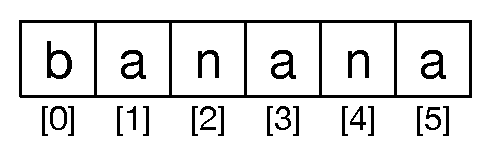
\includegraphics[keepaspectratio,alt={String Indexes},height=0.75in]{../images/string.eps}}
\caption{String Indexes}
\end{figure}

\index{index!starting at zero} \index{zero, index starting at}

Maaari mong gamitin ang anumang expression, kasama ang variables at
operators, bilang index, pero ang value ng index ay dapat integer. Kung
hindi makakakuha ka ng:

\index{index} \index{} \index{exception!TypeError} \index{TypeError}

\begin{Shaded}
\begin{Highlighting}[]
\OperatorTok{\textgreater{}\textgreater{}\textgreater{}}\NormalTok{ letter }\OperatorTok{=}\NormalTok{ fruit[}\FloatTok{1.5}\NormalTok{]}
\PreprocessorTok{TypeError}\NormalTok{: string indices must be integers}
\end{Highlighting}
\end{Shaded}

\section{\texorpdfstring{Getting the length of a string using
\texttt{len}}{Getting the length of a string using len}}\label{getting-the-length-of-a-string-using-len}

\index{len function} \index{function!len}

Ang \texttt{len} ay built-in function na nagre-return ng bilang ng
characters sa string:

\begin{Shaded}
\begin{Highlighting}[]
\OperatorTok{\textgreater{}\textgreater{}\textgreater{}}\NormalTok{ fruit }\OperatorTok{=} \StringTok{\textquotesingle{}banana\textquotesingle{}}
\OperatorTok{\textgreater{}\textgreater{}\textgreater{}} \BuiltInTok{len}\NormalTok{(fruit)}
\DecValTok{6}
\end{Highlighting}
\end{Shaded}

Para makuha ang huling letra ng string, maaari kang matukso na subukan
ang isang bagay na ganito:

\index{exception!IndexError} \index{IndexError}

\begin{Shaded}
\begin{Highlighting}[]
\OperatorTok{\textgreater{}\textgreater{}\textgreater{}}\NormalTok{ length }\OperatorTok{=} \BuiltInTok{len}\NormalTok{(fruit)}
\OperatorTok{\textgreater{}\textgreater{}\textgreater{}}\NormalTok{ last }\OperatorTok{=}\NormalTok{ fruit[length]}
\PreprocessorTok{IndexError}\NormalTok{: string index out of }\BuiltInTok{range}
\end{Highlighting}
\end{Shaded}

Ang dahilan ng \texttt{IndexError} ay walang letra sa ``banana'' na may
index 6. Dahil nagsimula tayo sa pagbilang sa zero, ang anim na letra ay
may numero 0 hanggang 5. Para makuha ang huling character, kailangan
mong ibawas ang 1 mula sa \texttt{length}:

\begin{Shaded}
\begin{Highlighting}[]
\OperatorTok{\textgreater{}\textgreater{}\textgreater{}}\NormalTok{ last }\OperatorTok{=}\NormalTok{ fruit[length}\OperatorTok{{-}}\DecValTok{1}\NormalTok{]}
\OperatorTok{\textgreater{}\textgreater{}\textgreater{}} \BuiltInTok{print}\NormalTok{(last)}
\NormalTok{a}
\end{Highlighting}
\end{Shaded}

Bilang alternatibo, maaari mong gamitin ang negative indices, na
nagbi-bilang pabalik mula sa dulo ng string. Ang expression na
\texttt{fruit{[}-1{]}} ay nagbibigay ng huling letra, ang
\texttt{fruit{[}-2{]}} ay nagbibigay ng pangalawang huli, at iba pa.

\index{index!negative} \index{negative index}

\section{Traversal through a string with a
loop}\label{traversal-through-a-string-with-a-loop}

\index{traversal} \index{loop!traversal} \index{for loop}
\index{loop!for} \index{statement!for} \index{traversal}

Maraming computations ang nagsasangkot ng pagproseso ng string isang
character sa isang panahon. Kadalasan nagsisimula sila sa simula,
pumipili ng bawat character nang sunud-sunod, gumagawa ng isang bagay
dito, at nagpapatuloy hanggang sa dulo. Ang pattern ng processing na ito
ay tinatawag na \emph{traversal}. Isang paraan para sumulat ng traversal
ay gamit ang \texttt{while} loop:

\begin{Shaded}
\begin{Highlighting}[]
\NormalTok{index }\OperatorTok{=} \DecValTok{0}
\ControlFlowTok{while}\NormalTok{ index }\OperatorTok{\textless{}} \BuiltInTok{len}\NormalTok{(fruit):}
\NormalTok{    letter }\OperatorTok{=}\NormalTok{ fruit[index]}
    \BuiltInTok{print}\NormalTok{(letter)}
\NormalTok{    index }\OperatorTok{=}\NormalTok{ index }\OperatorTok{+} \DecValTok{1}
\end{Highlighting}
\end{Shaded}

Ang loop na ito ay dumadaan sa string at nagdi-display ng bawat letra sa
isang linya na mag-isa. Ang loop condition ay
\texttt{index\ \textless{}\ len(fruit)}, kaya kapag ang \texttt{index}
ay katumbas ng haba ng string, ang condition ay false, at ang body ng
loop ay hindi na-e-execute. Ang huling character na na-access ay ang may
index na \texttt{len(fruit)-1}, na ang huling character sa string.

\textbf{Exercise 1:} Sumulat ng \texttt{while} loop na nagsisimula sa
huling character sa string at gumagana pabalik patungo sa unang
character sa string, na nagpi-print ng bawat letra sa hiwalay na linya,
maliban sa pabalik.

Ang isa pang paraan para sumulat ng traversal ay gamit ang \texttt{for}
loop:

\begin{Shaded}
\begin{Highlighting}[]
\ControlFlowTok{for}\NormalTok{ char }\KeywordTok{in}\NormalTok{ fruit:}
    \BuiltInTok{print}\NormalTok{(char)}
\end{Highlighting}
\end{Shaded}

Sa bawat pagkakataon sa loop, ang susunod na character sa string ay
na-a-assign sa variable na \texttt{char}. Ang loop ay nagpapatuloy
hanggang walang characters na natitira.

\section{String slices}\label{string-slices}

\index{slice operator} \index{operator!slice} \index{index!slice}
\index{string!slice} \index{slice!string}

Ang segment ng string ay tinatawag na \emph{slice}. Ang pagpili ng slice
ay katulad ng pagpili ng character:

\begin{Shaded}
\begin{Highlighting}[]
\OperatorTok{\textgreater{}\textgreater{}\textgreater{}}\NormalTok{ s }\OperatorTok{=} \StringTok{\textquotesingle{}Monty Python\textquotesingle{}}
\OperatorTok{\textgreater{}\textgreater{}\textgreater{}} \BuiltInTok{print}\NormalTok{(s[}\DecValTok{0}\NormalTok{:}\DecValTok{5}\NormalTok{])}
\NormalTok{Monty}
\OperatorTok{\textgreater{}\textgreater{}\textgreater{}} \BuiltInTok{print}\NormalTok{(s[}\DecValTok{6}\NormalTok{:}\DecValTok{12}\NormalTok{])}
\NormalTok{Python}
\end{Highlighting}
\end{Shaded}

Ang operator {[}n:m{]} ay nagre-return ng parte ng string mula sa
``n-th'' character hanggang sa ``m-th'' character, kasama ang una pero
hindi kasama ang huli.

Kung tatanggalin mo ang unang index (bago ang colon), ang slice ay
nagsisimula sa simula ng string. Kung tatanggalin mo ang pangalawang
index, ang slice ay hanggang sa dulo ng string:

\begin{Shaded}
\begin{Highlighting}[]
\OperatorTok{\textgreater{}\textgreater{}\textgreater{}}\NormalTok{ fruit }\OperatorTok{=} \StringTok{\textquotesingle{}banana\textquotesingle{}}
\OperatorTok{\textgreater{}\textgreater{}\textgreater{}}\NormalTok{ fruit[:}\DecValTok{3}\NormalTok{]}
\CommentTok{\textquotesingle{}ban\textquotesingle{}}
\OperatorTok{\textgreater{}\textgreater{}\textgreater{}}\NormalTok{ fruit[}\DecValTok{3}\NormalTok{:]}
\CommentTok{\textquotesingle{}ana\textquotesingle{}}
\end{Highlighting}
\end{Shaded}

Kung ang unang index ay mas malaki o katumbas ng pangalawa ang result ay
\emph{empty string}, na kinakatawan ng dalawang quotation marks:

\index{quotation mark}

\begin{Shaded}
\begin{Highlighting}[]
\OperatorTok{\textgreater{}\textgreater{}\textgreater{}}\NormalTok{ fruit }\OperatorTok{=} \StringTok{\textquotesingle{}banana\textquotesingle{}}
\OperatorTok{\textgreater{}\textgreater{}\textgreater{}}\NormalTok{ fruit[}\DecValTok{3}\NormalTok{:}\DecValTok{3}\NormalTok{]}
\CommentTok{\textquotesingle{}\textquotesingle{}}
\end{Highlighting}
\end{Shaded}

Ang empty string ay walang characters at may haba na 0, pero bukod sa
iyon, pareho ito sa anumang iba pang string.

\textbf{Exercise 2:} Given na ang \texttt{fruit} ay string, ano ang ibig
sabihin ng \texttt{fruit{[}:{]}}?

\index{copy!slice} \index{slice!copy}

\section{Strings are immutable}\label{strings-are-immutable}

\index{mutability} \index{immutability} \index{string!immutable}

Nakakatukso na gamitin ang operator sa kaliwang bahagi ng assignment, na
may layunin na baguhin ang character sa string. Halimbawa:

\index{TypeError} \index{exception!TypeError}

\begin{Shaded}
\begin{Highlighting}[]
\OperatorTok{\textgreater{}\textgreater{}\textgreater{}}\NormalTok{ greeting }\OperatorTok{=} \StringTok{\textquotesingle{}Hello, world!\textquotesingle{}}
\OperatorTok{\textgreater{}\textgreater{}\textgreater{}}\NormalTok{ greeting[}\DecValTok{0}\NormalTok{] }\OperatorTok{=} \StringTok{\textquotesingle{}J\textquotesingle{}}
\PreprocessorTok{TypeError}\NormalTok{: }\StringTok{\textquotesingle{}str\textquotesingle{}} \BuiltInTok{object}\NormalTok{ does }\KeywordTok{not}\NormalTok{ support item assignment}
\end{Highlighting}
\end{Shaded}

Ang ``object'' sa kasong ito ay ang string at ang ``item'' ay ang
character na sinubukan mong i-assign. Sa ngayon, ang \emph{object} ay
pareho sa value, pero pipino natin ang definition na iyon mamaya. Ang
\emph{item} ay isa sa mga values sa sequence.

\index{object} \index{item assignment} \index{assignment!item}
\index{immutability}

Ang dahilan ng error ay ang strings ay \emph{immutable}, na
nangangahulugang hindi mo maaaring baguhin ang existing string. Ang
pinakamabuting magagawa mo ay gumawa ng bagong string na variation ng
original:

\begin{Shaded}
\begin{Highlighting}[]
\OperatorTok{\textgreater{}\textgreater{}\textgreater{}}\NormalTok{ greeting }\OperatorTok{=} \StringTok{\textquotesingle{}Hello, world!\textquotesingle{}}
\OperatorTok{\textgreater{}\textgreater{}\textgreater{}}\NormalTok{ new\_greeting }\OperatorTok{=} \StringTok{\textquotesingle{}J\textquotesingle{}} \OperatorTok{+}\NormalTok{ greeting[}\DecValTok{1}\NormalTok{:]}
\OperatorTok{\textgreater{}\textgreater{}\textgreater{}} \BuiltInTok{print}\NormalTok{(new\_greeting)}
\NormalTok{Jello, world}\OperatorTok{!}
\end{Highlighting}
\end{Shaded}

Ang halimbawang ito ay nagko-concatenate ng bagong unang letra sa slice
ng \texttt{greeting}. Walang epekto ito sa original string.

\index{concatenation}

\section{Looping and counting}\label{looping-and-counting}

\index{counter} \index{counting and looping}
\index{looping and counting} \index{looping!with strings}

Ang sumusunod na program ay nagbi-bilang ng bilang ng beses na ang letra
``a'' ay lumalabas sa string:

\begin{Shaded}
\begin{Highlighting}[]
\NormalTok{word }\OperatorTok{=} \StringTok{\textquotesingle{}banana\textquotesingle{}}
\NormalTok{count }\OperatorTok{=} \DecValTok{0}
\ControlFlowTok{for}\NormalTok{ letter }\KeywordTok{in}\NormalTok{ word:}
    \ControlFlowTok{if}\NormalTok{ letter }\OperatorTok{==} \StringTok{\textquotesingle{}a\textquotesingle{}}\NormalTok{:}
\NormalTok{        count }\OperatorTok{=}\NormalTok{ count }\OperatorTok{+} \DecValTok{1}
\BuiltInTok{print}\NormalTok{(count)}
\end{Highlighting}
\end{Shaded}

Ang program na ito ay nagpapakita ng isa pang pattern ng computation na
tinatawag na \emph{counter}. Ang variable na \texttt{count} ay
ini-initialize sa 0 at pagkatapos i-increment sa bawat pagkakataon na
makikita ang ``a''. Kapag ang loop ay lumabas, ang \texttt{count} ay
naglalaman ng result: ang kabuuang bilang ng a's.

\index{encapsulation}

\textbf{Exercise 3:} I-encapsulate ang code na ito sa function na may
pangalang \texttt{count}, at gawing general para tumanggap ng string at
letra bilang arguments.

\section{\texorpdfstring{The \texttt{in}
operator}{The in operator}}\label{the-in-operator}

\index{in operator} \index{operator!in} \index{boolean operator}
\index{operator!boolean}

Ang salitang \texttt{in} ay boolean operator na tumatanggap ng dalawang
strings at nagre-return ng \texttt{True} kung ang una ay lumalabas
bilang substring sa pangalawa:

\begin{Shaded}
\begin{Highlighting}[]
\OperatorTok{\textgreater{}\textgreater{}\textgreater{}} \StringTok{\textquotesingle{}a\textquotesingle{}} \KeywordTok{in} \StringTok{\textquotesingle{}banana\textquotesingle{}}
\VariableTok{True}
\OperatorTok{\textgreater{}\textgreater{}\textgreater{}} \StringTok{\textquotesingle{}seed\textquotesingle{}} \KeywordTok{in} \StringTok{\textquotesingle{}banana\textquotesingle{}}
\VariableTok{False}
\end{Highlighting}
\end{Shaded}

\section{String comparison}\label{string-comparison}

\index{string!comparison} \index{comparison!string}

Ang comparison operators ay gumagana sa strings. Para makita kung ang
dalawang strings ay equal:

\begin{Shaded}
\begin{Highlighting}[]
\ControlFlowTok{if}\NormalTok{ word }\OperatorTok{==} \StringTok{\textquotesingle{}banana\textquotesingle{}}\NormalTok{:}
    \BuiltInTok{print}\NormalTok{(}\StringTok{\textquotesingle{}All right, bananas.\textquotesingle{}}\NormalTok{)}
\end{Highlighting}
\end{Shaded}

Ang iba pang comparison operations ay kapaki-pakinabang para ilagay ang
mga salita sa alphabetical order:

\begin{Shaded}
\begin{Highlighting}[]
\ControlFlowTok{if}\NormalTok{ word }\OperatorTok{\textless{}} \StringTok{\textquotesingle{}banana\textquotesingle{}}\NormalTok{:}
    \BuiltInTok{print}\NormalTok{(}\StringTok{\textquotesingle{}Your word,\textquotesingle{}} \OperatorTok{+}\NormalTok{ word }\OperatorTok{+} \StringTok{\textquotesingle{}, comes before banana.\textquotesingle{}}\NormalTok{)}
\ControlFlowTok{elif}\NormalTok{ word }\OperatorTok{\textgreater{}} \StringTok{\textquotesingle{}banana\textquotesingle{}}\NormalTok{:}
    \BuiltInTok{print}\NormalTok{(}\StringTok{\textquotesingle{}Your word,\textquotesingle{}} \OperatorTok{+}\NormalTok{ word }\OperatorTok{+} \StringTok{\textquotesingle{}, comes after banana.\textquotesingle{}}\NormalTok{)}
\ControlFlowTok{else}\NormalTok{:}
    \BuiltInTok{print}\NormalTok{(}\StringTok{\textquotesingle{}All right, bananas.\textquotesingle{}}\NormalTok{)}
\end{Highlighting}
\end{Shaded}

Ang Python ay hindi nagha-handle ng uppercase at lowercase letters sa
parehong paraan na ginagawa ng mga tao. Lahat ng uppercase letters ay
nauuna sa lahat ng lowercase letters, kaya:

{\small
\begin{verbatim}
Your word, Pineapple, comes before banana.
\end{verbatim}
}

Karaniwang paraan para solusyonan ang problemang ito ay i-convert ang
strings sa standard format, tulad ng lahat lowercase, bago gawin ang
comparison. Tandaan iyon kung sakaling kailangan mong ipagtanggol ang
sarili mo laban sa taong armado ng Pineapple.

\section{String methods}\label{string-methods}

Ang Strings ay halimbawa ng Python \emph{objects}. Ang object ay
naglalaman ng parehong data (ang actual string mismo) at \emph{methods},
na epektibong functions na built sa object at available sa anumang
\emph{instance} ng object.

Ang Python ay may function na tinatawag na \texttt{dir} na nagli-list ng
methods available para sa object. Ang \texttt{type} function ay
nagpapakita ng type ng object at ang \texttt{dir} function ay
nagpapakita ng available methods.

\begin{Shaded}
\begin{Highlighting}[]
\OperatorTok{\textgreater{}\textgreater{}\textgreater{}}\NormalTok{ stuff }\OperatorTok{=} \StringTok{\textquotesingle{}Hello world\textquotesingle{}}
\OperatorTok{\textgreater{}\textgreater{}\textgreater{}} \BuiltInTok{type}\NormalTok{(stuff)}
\OperatorTok{\textless{}}\KeywordTok{class} \StringTok{\textquotesingle{}str\textquotesingle{}}\OperatorTok{\textgreater{}}
\OperatorTok{\textgreater{}\textgreater{}\textgreater{}} \BuiltInTok{dir}\NormalTok{(stuff)}
\NormalTok{[... }\StringTok{\textquotesingle{}capitalize\textquotesingle{}}\NormalTok{, }\StringTok{\textquotesingle{}casefold\textquotesingle{}}\NormalTok{, }\StringTok{\textquotesingle{}center\textquotesingle{}}\NormalTok{, }\StringTok{\textquotesingle{}count\textquotesingle{}}\NormalTok{, }\StringTok{\textquotesingle{}encode\textquotesingle{}}\NormalTok{,}
\StringTok{\textquotesingle{}endswith\textquotesingle{}}\NormalTok{, }\StringTok{\textquotesingle{}expandtabs\textquotesingle{}}\NormalTok{, }\StringTok{\textquotesingle{}find\textquotesingle{}}\NormalTok{, }\StringTok{\textquotesingle{}format\textquotesingle{}}\NormalTok{, }\StringTok{\textquotesingle{}format\_map\textquotesingle{}}\NormalTok{,}
\StringTok{\textquotesingle{}index\textquotesingle{}}\NormalTok{, }\StringTok{\textquotesingle{}isalnum\textquotesingle{}}\NormalTok{, }\StringTok{\textquotesingle{}isalpha\textquotesingle{}}\NormalTok{, }\StringTok{\textquotesingle{}isdecimal\textquotesingle{}}\NormalTok{, }\StringTok{\textquotesingle{}isdigit\textquotesingle{}}\NormalTok{,}
\StringTok{\textquotesingle{}isidentifier\textquotesingle{}}\NormalTok{, }\StringTok{\textquotesingle{}islower\textquotesingle{}}\NormalTok{, }\StringTok{\textquotesingle{}isnumeric\textquotesingle{}}\NormalTok{, }\StringTok{\textquotesingle{}isprintable\textquotesingle{}}\NormalTok{,}
\StringTok{\textquotesingle{}isspace\textquotesingle{}}\NormalTok{, }\StringTok{\textquotesingle{}istitle\textquotesingle{}}\NormalTok{, }\StringTok{\textquotesingle{}isupper\textquotesingle{}}\NormalTok{, }\StringTok{\textquotesingle{}join\textquotesingle{}}\NormalTok{, }\StringTok{\textquotesingle{}ljust\textquotesingle{}}\NormalTok{, }\StringTok{\textquotesingle{}lower\textquotesingle{}}\NormalTok{,}
\StringTok{\textquotesingle{}lstrip\textquotesingle{}}\NormalTok{, }\StringTok{\textquotesingle{}maketrans\textquotesingle{}}\NormalTok{, }\StringTok{\textquotesingle{}partition\textquotesingle{}}\NormalTok{, }\StringTok{\textquotesingle{}replace\textquotesingle{}}\NormalTok{, }\StringTok{\textquotesingle{}rfind\textquotesingle{}}\NormalTok{,}
\StringTok{\textquotesingle{}rindex\textquotesingle{}}\NormalTok{, }\StringTok{\textquotesingle{}rjust\textquotesingle{}}\NormalTok{, }\StringTok{\textquotesingle{}rpartition\textquotesingle{}}\NormalTok{, }\StringTok{\textquotesingle{}rsplit\textquotesingle{}}\NormalTok{, }\StringTok{\textquotesingle{}rstrip\textquotesingle{}}\NormalTok{,}
\StringTok{\textquotesingle{}split\textquotesingle{}}\NormalTok{, }\StringTok{\textquotesingle{}splitlines\textquotesingle{}}\NormalTok{, }\StringTok{\textquotesingle{}startswith\textquotesingle{}}\NormalTok{, }\StringTok{\textquotesingle{}strip\textquotesingle{}}\NormalTok{, }\StringTok{\textquotesingle{}swapcase\textquotesingle{}}\NormalTok{,}
\StringTok{\textquotesingle{}title\textquotesingle{}}\NormalTok{, }\StringTok{\textquotesingle{}translate\textquotesingle{}}\NormalTok{, }\StringTok{\textquotesingle{}upper\textquotesingle{}}\NormalTok{, }\StringTok{\textquotesingle{}zfill\textquotesingle{}}\NormalTok{]}
\OperatorTok{\textgreater{}\textgreater{}\textgreater{}} \BuiltInTok{help}\NormalTok{(}\BuiltInTok{str}\NormalTok{.capitalize)}
\NormalTok{Help on method\_descriptor:}

\NormalTok{capitalize(}\VariableTok{self}\NormalTok{, }\OperatorTok{/}\NormalTok{)}
\NormalTok{    Return a capitalized version of the string.}
    
\NormalTok{    More specifically, make the first character have upper}
    \ControlFlowTok{case} \KeywordTok{and}\NormalTok{ the rest lower case.}
\OperatorTok{\textgreater{}\textgreater{}\textgreater{}}
\end{Highlighting}
\end{Shaded}

Habang ang \texttt{dir} function ay nagli-list ng methods, at maaari
mong gamitin ang \texttt{help} para makakuha ng ilang simpleng
documentation sa method, mas mabuting source ng documentation para sa
string methods ay

\url{https://docs.python.org/library/stdtypes.html\#string-methods}.

Ang pagtawag sa \emph{method} ay katulad ng pagtawag sa function (ito ay
tumatanggap ng arguments at nagre-return ng value) pero ang syntax ay
iba. Tinatawag natin ang method sa pamamagitan ng pag-append ng method
name sa variable name gamit ang period bilang delimiter.

Halimbawa, ang method na \texttt{upper} ay tumatanggap ng string at
nagre-return ng bagong string na may lahat uppercase letters:

\index{method} \index{string!method}

Sa halip na function syntax na \texttt{upper(word)}, ginagamit nito ang
method syntax na \texttt{word.upper()}.

\index{dot notation}

\begin{Shaded}
\begin{Highlighting}[]
\OperatorTok{\textgreater{}\textgreater{}\textgreater{}}\NormalTok{ word }\OperatorTok{=} \StringTok{\textquotesingle{}banana\textquotesingle{}}
\OperatorTok{\textgreater{}\textgreater{}\textgreater{}}\NormalTok{ new\_word }\OperatorTok{=}\NormalTok{ word.upper()}
\OperatorTok{\textgreater{}\textgreater{}\textgreater{}} \BuiltInTok{print}\NormalTok{(new\_word)}
\NormalTok{BANANA}
\end{Highlighting}
\end{Shaded}

Ang form ng dot notation na ito ay tumutukoy sa pangalan ng method,
\texttt{upper}, at ang pangalan ng string na a-applyan ng method,
\texttt{word}. Ang empty parentheses ay nagpapahiwatig na ang method na
ito ay hindi tumatanggap ng argument.

\index{parentheses!empty}

Ang method call ay tinatawag na \emph{invocation}; sa kasong ito,
sasabihin natin na nag-i-invoke tayo ng \texttt{upper} sa \texttt{word}.

\index{invocation}

Halimbawa, mayroong string method na may pangalang \texttt{find} na
naghahanap ng posisyon ng isang string sa loob ng isa pa:

\begin{Shaded}
\begin{Highlighting}[]
\OperatorTok{\textgreater{}\textgreater{}\textgreater{}}\NormalTok{ word }\OperatorTok{=} \StringTok{\textquotesingle{}banana\textquotesingle{}}
\OperatorTok{\textgreater{}\textgreater{}\textgreater{}}\NormalTok{ index }\OperatorTok{=}\NormalTok{ word.find(}\StringTok{\textquotesingle{}a\textquotesingle{}}\NormalTok{)}
\OperatorTok{\textgreater{}\textgreater{}\textgreater{}} \BuiltInTok{print}\NormalTok{(index)}
\DecValTok{1}
\end{Highlighting}
\end{Shaded}

Sa halimbawang ito, nag-i-invoke tayo ng \texttt{find} sa \texttt{word}
at ipinapasa ang letra na hinahanap natin bilang parameter.

Ang \texttt{find} method ay maaaring makahanap ng substrings pati na rin
characters:

\begin{Shaded}
\begin{Highlighting}[]
\OperatorTok{\textgreater{}\textgreater{}\textgreater{}}\NormalTok{ word.find(}\StringTok{\textquotesingle{}na\textquotesingle{}}\NormalTok{)}
\DecValTok{2}
\end{Highlighting}
\end{Shaded}

Maaari itong tumanggap bilang pangalawang argument ng index kung saan
dapat ito magsimula:

\index{optional argument} \index{argument!optional}

\begin{Shaded}
\begin{Highlighting}[]
\OperatorTok{\textgreater{}\textgreater{}\textgreater{}}\NormalTok{ word.find(}\StringTok{\textquotesingle{}na\textquotesingle{}}\NormalTok{, }\DecValTok{3}\NormalTok{)}
\DecValTok{4}
\end{Highlighting}
\end{Shaded}

Isang karaniwang gawain ay alisin ang white space (spaces, tabs, o
newlines) mula sa simula at dulo ng string gamit ang \texttt{strip}
method:

\begin{Shaded}
\begin{Highlighting}[]
\OperatorTok{\textgreater{}\textgreater{}\textgreater{}}\NormalTok{ line }\OperatorTok{=} \StringTok{\textquotesingle{}  Here we go  \textquotesingle{}}
\OperatorTok{\textgreater{}\textgreater{}\textgreater{}}\NormalTok{ line.strip()}
\CommentTok{\textquotesingle{}Here we go\textquotesingle{}}
\end{Highlighting}
\end{Shaded}

Ang ilang methods tulad ng \emph{startswith} ay nagre-return ng boolean
values.

\begin{Shaded}
\begin{Highlighting}[]
\OperatorTok{\textgreater{}\textgreater{}\textgreater{}}\NormalTok{ line }\OperatorTok{=} \StringTok{\textquotesingle{}Have a nice day\textquotesingle{}}
\OperatorTok{\textgreater{}\textgreater{}\textgreater{}}\NormalTok{ line.startswith(}\StringTok{\textquotesingle{}Have\textquotesingle{}}\NormalTok{)}
\VariableTok{True}
\OperatorTok{\textgreater{}\textgreater{}\textgreater{}}\NormalTok{ line.startswith(}\StringTok{\textquotesingle{}h\textquotesingle{}}\NormalTok{)}
\VariableTok{False}
\end{Highlighting}
\end{Shaded}

Mapapansin mo na ang \texttt{startswith} ay nangangailangan ng case na
tumugma, kaya minsan kumukuha tayo ng linya at i-map ito lahat sa
lowercase bago gumawa ng anumang checking gamit ang \texttt{lower}
method.

\begin{Shaded}
\begin{Highlighting}[]
\OperatorTok{\textgreater{}\textgreater{}\textgreater{}}\NormalTok{ line }\OperatorTok{=} \StringTok{\textquotesingle{}Have a nice day\textquotesingle{}}
\OperatorTok{\textgreater{}\textgreater{}\textgreater{}}\NormalTok{ line.startswith(}\StringTok{\textquotesingle{}h\textquotesingle{}}\NormalTok{)}
\VariableTok{False}
\OperatorTok{\textgreater{}\textgreater{}\textgreater{}}\NormalTok{ line.lower()}
\CommentTok{\textquotesingle{}have a nice day\textquotesingle{}}
\OperatorTok{\textgreater{}\textgreater{}\textgreater{}}\NormalTok{ line.lower().startswith(}\StringTok{\textquotesingle{}h\textquotesingle{}}\NormalTok{)}
\VariableTok{True}
\end{Highlighting}
\end{Shaded}

Sa huling halimbawa, ang method na \texttt{lower} ay tinatawag at
pagkatapos ginagamit natin ang \texttt{startswith} para makita kung ang
resulting lowercase string ay nagsisimula sa letrang ``h''. Hangga't
maingat tayo sa order, maaari tayong gumawa ng maraming method calls sa
isang expression.

\index{count method} \index{method!count}

\textbf{Exercise 4:} Mayroong string method na tinatawag na
\texttt{count} na katulad ng function sa naunang exercise. Basahin ang
documentation ng method na ito sa:

\url{https://docs.python.org/library/stdtypes.html\#string-methods}

Sumulat ng invocation na nagbi-bilang ng bilang ng beses na ang letrang
a ay nangyayari sa ``banana''.

\section{Parsing strings}\label{parsing-strings}

Kadalasan, gusto nating tumingin sa string at makahanap ng substring.
Halimbawa kung ipinakita sa atin ang serye ng mga linya na na-format
tulad ng sumusunod:

\texttt{From\ stephen.marquard@}\emph{\texttt{uct.ac.za}}\texttt{Sat\ Jan\ \ 5\ 09:14:16\ 2008}

at gusto nating kunin lang ang pangalawang kalahati ng address (i.e.,
\texttt{uct.ac.za}) mula sa bawat linya, maaari nating gawin ito sa
pamamagitan ng paggamit ng \texttt{find} method at string slicing.

Una, hahanapin natin ang posisyon ng at-sign sa string. Pagkatapos
hahanapin natin ang posisyon ng unang space \emph{pagkatapos} ng
at-sign. At pagkatapos gagamitin natin ang string slicing para kunin ang
parte ng string na hinahanap natin.

\begin{Shaded}
\begin{Highlighting}[]
\OperatorTok{\textgreater{}\textgreater{}\textgreater{}}\NormalTok{ data }\OperatorTok{=} \StringTok{\textquotesingle{}From stephen.marquard@uct.ac.za Sat Jan  5 09:14:16 2008\textquotesingle{}}
\OperatorTok{\textgreater{}\textgreater{}\textgreater{}}\NormalTok{ atpos }\OperatorTok{=}\NormalTok{ data.find(}\StringTok{\textquotesingle{}@\textquotesingle{}}\NormalTok{)}
\OperatorTok{\textgreater{}\textgreater{}\textgreater{}} \BuiltInTok{print}\NormalTok{(atpos)}
\DecValTok{21}
\OperatorTok{\textgreater{}\textgreater{}\textgreater{}}\NormalTok{ sppos }\OperatorTok{=}\NormalTok{ data.find(}\StringTok{\textquotesingle{} \textquotesingle{}}\NormalTok{,atpos)}
\OperatorTok{\textgreater{}\textgreater{}\textgreater{}} \BuiltInTok{print}\NormalTok{(sppos)}
\DecValTok{31}
\OperatorTok{\textgreater{}\textgreater{}\textgreater{}}\NormalTok{ host }\OperatorTok{=}\NormalTok{ data[atpos}\OperatorTok{+}\DecValTok{1}\NormalTok{:sppos]}
\OperatorTok{\textgreater{}\textgreater{}\textgreater{}} \BuiltInTok{print}\NormalTok{(host)}
\NormalTok{uct.ac.za}
\OperatorTok{\textgreater{}\textgreater{}\textgreater{}}
\end{Highlighting}
\end{Shaded}

Ginagamit natin ang bersyon ng \texttt{find} method na nagpapahintulot
sa atin na tukuyin ang posisyon sa string kung saan gusto nating
magsimulang maghanap ang \texttt{find}. Kapag nag-slice tayo, kinukuha
natin ang characters mula sa ``isa pagkatapos ng at-sign hanggang sa
\emph{pero hindi kasama} ang space character''.

Ang documentation para sa \texttt{find} method ay available sa

\url{https://docs.python.org/library/stdtypes.html\#string-methods}.

\section{Formatted String Literals}\label{formatted-string-literals}

\index{formatted string literals}

Ang formatted string literal (kadalasang tinutukoy lang bilang f-string)
ay nagpapahintulot na gamitin ang Python expressions sa loob ng string
literals. Ito ay nakakamit sa pamamagitan ng pag-prepend ng \texttt{f}
sa string literal at pag-enclose ng expressions sa curly braces
\texttt{\{\}}.

Halimbawa, ang pag-wrap ng variable name sa curly braces sa loob ng
f-string ay magdudulot na mapalitan ito ng value nito:

\begin{Shaded}
\begin{Highlighting}[]
\OperatorTok{\textgreater{}\textgreater{}\textgreater{}}\NormalTok{ camels }\OperatorTok{=} \DecValTok{42}
\OperatorTok{\textgreater{}\textgreater{}\textgreater{}} \SpecialStringTok{f\textquotesingle{}}\SpecialCharTok{\{}\NormalTok{camels}\SpecialCharTok{\}}\SpecialStringTok{\textquotesingle{}}
\CommentTok{\textquotesingle{}42\textquotesingle{}}
\end{Highlighting}
\end{Shaded}

Ang result ay ang string na `42', na hindi dapat malito sa integer value
na 42.

Ang expression ay maaaring lumabas kahit saan sa string, kaya maaari
mong i-embed ang value sa sentence:

\begin{Shaded}
\begin{Highlighting}[]
\OperatorTok{\textgreater{}\textgreater{}\textgreater{}}\NormalTok{ camels }\OperatorTok{=} \DecValTok{42}
\OperatorTok{\textgreater{}\textgreater{}\textgreater{}} \SpecialStringTok{f\textquotesingle{}I have spotted }\SpecialCharTok{\{}\NormalTok{camels}\SpecialCharTok{\}}\SpecialStringTok{ camels.\textquotesingle{}}
\CommentTok{\textquotesingle{}I have spotted 42 camels.\textquotesingle{}}
\end{Highlighting}
\end{Shaded}

Maraming expressions ay maaaring isama sa loob ng isang string literal
para gumawa ng mas kumplikadong strings.

\begin{Shaded}
\begin{Highlighting}[]
\OperatorTok{\textgreater{}\textgreater{}\textgreater{}}\NormalTok{ years }\OperatorTok{=} \DecValTok{3}
\OperatorTok{\textgreater{}\textgreater{}\textgreater{}}\NormalTok{ count }\OperatorTok{=} \FloatTok{.1}
\OperatorTok{\textgreater{}\textgreater{}\textgreater{}}\NormalTok{ species }\OperatorTok{=} \StringTok{\textquotesingle{}camels\textquotesingle{}}
\OperatorTok{\textgreater{}\textgreater{}\textgreater{}} \SpecialStringTok{f\textquotesingle{}In }\SpecialCharTok{\{}\NormalTok{years}\SpecialCharTok{\}}\SpecialStringTok{ years I have spotted }\SpecialCharTok{\{}\NormalTok{count}\SpecialCharTok{\}}\SpecialStringTok{ }\SpecialCharTok{\{}\NormalTok{species}\SpecialCharTok{\}}\SpecialStringTok{.\textquotesingle{}}
\CommentTok{\textquotesingle{}In 3 years I have spotted 0.1 camels.\textquotesingle{}}
\end{Highlighting}
\end{Shaded}

Ang formatted string literals ay makapangyarihan, at maaari silang
gumawa ng higit pa sa sakop dito. Maaari kang magbasa pa tungkol sa
kanila sa

\url{https://docs.python.org/3/tutorial/inputoutput.html\#formatted-string-literals}.

\section{Debugging}\label{debugging-5}

\index{debugging}

Isang skill na dapat mong linangin habang nagpo-program ay palaging
nagtatanong sa sarili, ``Ano ang maaaring maging mali dito?'' o bilang
alternatibo, ``Anong baliw na bagay ang maaaring gawin ng user natin
para i-crash ang (mukhang) perpektong program natin?''

Halimbawa, tingnan ang program na ginamit natin para ipakita ang
\texttt{while} loop sa chapter tungkol sa iteration:

\begin{Shaded}
\begin{Highlighting}[]
\ControlFlowTok{while} \VariableTok{True}\NormalTok{:}
\NormalTok{    line }\OperatorTok{=} \BuiltInTok{input}\NormalTok{(}\StringTok{\textquotesingle{}\textgreater{} \textquotesingle{}}\NormalTok{)}
    \ControlFlowTok{if}\NormalTok{ line[}\DecValTok{0}\NormalTok{] }\OperatorTok{==} \StringTok{\textquotesingle{}\#\textquotesingle{}}\NormalTok{:}
        \ControlFlowTok{continue}
    \ControlFlowTok{if}\NormalTok{ line }\OperatorTok{==} \StringTok{\textquotesingle{}done\textquotesingle{}}\NormalTok{:}
        \ControlFlowTok{break}
    \BuiltInTok{print}\NormalTok{(line)}
\BuiltInTok{print}\NormalTok{(}\StringTok{\textquotesingle{}Done!\textquotesingle{}}\NormalTok{)}

\CommentTok{\# Code: https://www.py4e.com/code3/copytildone2.py}
\end{Highlighting}
\end{Shaded}

Tingnan kung ano ang mangyayari kapag ang user ay nag-e-enter ng empty
line ng input:

\begin{Shaded}
\begin{Highlighting}[]
\OperatorTok{\textgreater{}}\NormalTok{ hello there}
\NormalTok{hello there}
\OperatorTok{\textgreater{}} \CommentTok{\# don\textquotesingle{}t print this}
\OperatorTok{\textgreater{}} \BuiltInTok{print}\NormalTok{ this}\OperatorTok{!}
\BuiltInTok{print}\NormalTok{ this}\OperatorTok{!}
\OperatorTok{\textgreater{}}
\NormalTok{Traceback (most recent call last):}
\NormalTok{  File }\StringTok{"copytildone.py"}\NormalTok{, line }\DecValTok{3}\NormalTok{, }\KeywordTok{in} \OperatorTok{\textless{}}\NormalTok{module}\OperatorTok{\textgreater{}}
    \ControlFlowTok{if}\NormalTok{ line[}\DecValTok{0}\NormalTok{] }\OperatorTok{==} \StringTok{\textquotesingle{}\#\textquotesingle{}}\NormalTok{:}
\PreprocessorTok{IndexError}\NormalTok{: string index out of }\BuiltInTok{range}
\end{Highlighting}
\end{Shaded}

Ang code ay gumagana nang maayos hanggang ipinakita ang empty line.
Pagkatapos walang zero-th character, kaya nakakakuha tayo ng traceback.
Mayroong dalawang solusyon sa ito para gawing ``safe'' ang line three
kahit na ang linya ay empty.

Ang isang posibilidad ay simpleng gamitin ang \texttt{startswith} method
na nagre-return ng \texttt{False} kung ang string ay empty.

\begin{Shaded}
\begin{Highlighting}[]
\ControlFlowTok{if}\NormalTok{ line.startswith(}\StringTok{\textquotesingle{}\#\textquotesingle{}}\NormalTok{):}
\end{Highlighting}
\end{Shaded}

\index{guardian pattern} \index{pattern!guardian}

Ang isa pang paraan ay ligtas na sumulat ng \texttt{if} statement gamit
ang \emph{guardian} pattern at siguraduhin na ang pangalawang logical
expression ay na-e-evaluate lang kung saan may hindi bababa sa isang
character sa string:

\begin{Shaded}
\begin{Highlighting}[]
\ControlFlowTok{if} \BuiltInTok{len}\NormalTok{(line) }\OperatorTok{\textgreater{}} \DecValTok{0} \KeywordTok{and}\NormalTok{ line[}\DecValTok{0}\NormalTok{] }\OperatorTok{==} \StringTok{\textquotesingle{}\#\textquotesingle{}}\NormalTok{:}
\end{Highlighting}
\end{Shaded}

\section{Glossary}\label{glossary-5}

\begin{description}
\tightlist
\item[counter]
Variable na ginagamit para bilangin ang isang bagay, karaniwang
ini-initialize sa zero at pagkatapos i-increment. \index{counter}
\item[empty string]
String na walang characters at may haba na 0, na kinakatawan ng dalawang
quotation marks. \index{empty string}
\item[flag]
Boolean variable na ginagamit para ipahiwatig kung ang condition ay true
o false. \index{flag}
\item[invocation]
Statement na tumatawag sa method. \index{invocation}
\item[immutable]
Ang property ng sequence na ang items ay hindi maaaring i-assign.
\index{immutability}
\item[index]
Integer value na ginagamit para pumili ng item sa sequence, tulad ng
character sa string. \index{index} \index{}
\item[item]
Isa sa mga values sa sequence. \index{item}
\item[method]
Function na nauugnay sa object at tinatawag gamit ang dot notation.
\index{method}
\item[object]
Isang bagay na maaaring tinukoy ng variable. Sa ngayon, maaari mong
gamitin ang ``object'' at ``value'' nang magkakapalit. \index{object}
\item[search]
Pattern ng traversal na humihinto kapag nakita na ang hinahanap nito.
\index{search pattern} \index{pattern!search}
\item[sequence]
Ordered set; iyon ay, set ng values kung saan ang bawat value ay
nakikilala ng integer index. \index{sequence}
\item[slice]
Parte ng string na tinukoy ng range ng indices. \index{slice}
\item[traverse]
Mag-iterate sa mga items sa sequence, na gumagawa ng katulad na
operation sa bawat isa. \index{traversal}
\end{description}

\section{Exercises}\label{exercises-5}

\textbf{Exercise 5:} Slicing strings

Kunin ang sumusunod na Python code na nag-i-store ng string:

\texttt{str\ =\ \textquotesingle{}X-DSPAM-Confidence:\ 0.8475\textquotesingle{}}

Gamitin ang \texttt{find} at string slicing para kunin ang parte ng
string pagkatapos ng colon character at pagkatapos gamitin ang
\texttt{float} function para i-convert ang extracted string sa floating
point number.

\index{string method} \index{method!string}

\textbf{Exercise 6:} String methods

Basahin ang documentation ng string methods sa

\url{https://docs.python.org/library/stdtypes.html\#string-methods}.

Maaaring gusto mong mag-eksperimento sa ilan sa kanila para masiguro na
naiintindihan mo kung paano sila gumagana. Ang \texttt{strip} at
\texttt{replace} ay partikular na kapaki-pakinabang.

Ang documentation ay gumagamit ng syntax na maaaring nakakalito.
Halimbawa, sa \texttt{find(sub{[},\ start{[},\ end{]}{]})}, ang brackets
ay nagpapahiwatig ng optional arguments. Kaya ang \texttt{sub} ay
required, pero ang \texttt{start} ay optional, at kung isasama mo ang
\texttt{start}, pagkatapos ang \texttt{end} ay optional.

\chapter{Files}\label{files}

\index{file} \index{type!file}

\section{Persistence}\label{persistence}

\index{persistence} \index{secondary memory}

Hanggang ngayon, natutunan natin kung paano sumulat ng programs at
makipag-ugnayan sa intentions natin sa \emph{Central Processing Unit}
gamit ang conditional execution, functions, at iterations. Natutunan
natin kung paano gumawa at gumamit ng data structures sa \emph{Main
Memory}. Ang CPU at memory ay kung saan gumagana at tumatakbo ang
software natin. Ito ay kung saan lahat ng ``pag-iisip'' ay nangyayari.

Pero kung maaalala mo mula sa hardware architecture discussions natin,
kapag ang power ay naka-off, anumang naka-store sa CPU o main memory ay
nabubura. Kaya hanggang ngayon, ang mga programs natin ay simpleng
transient fun exercises lang para matuto ng Python.

\begin{figure}
\centering
\pandocbounded{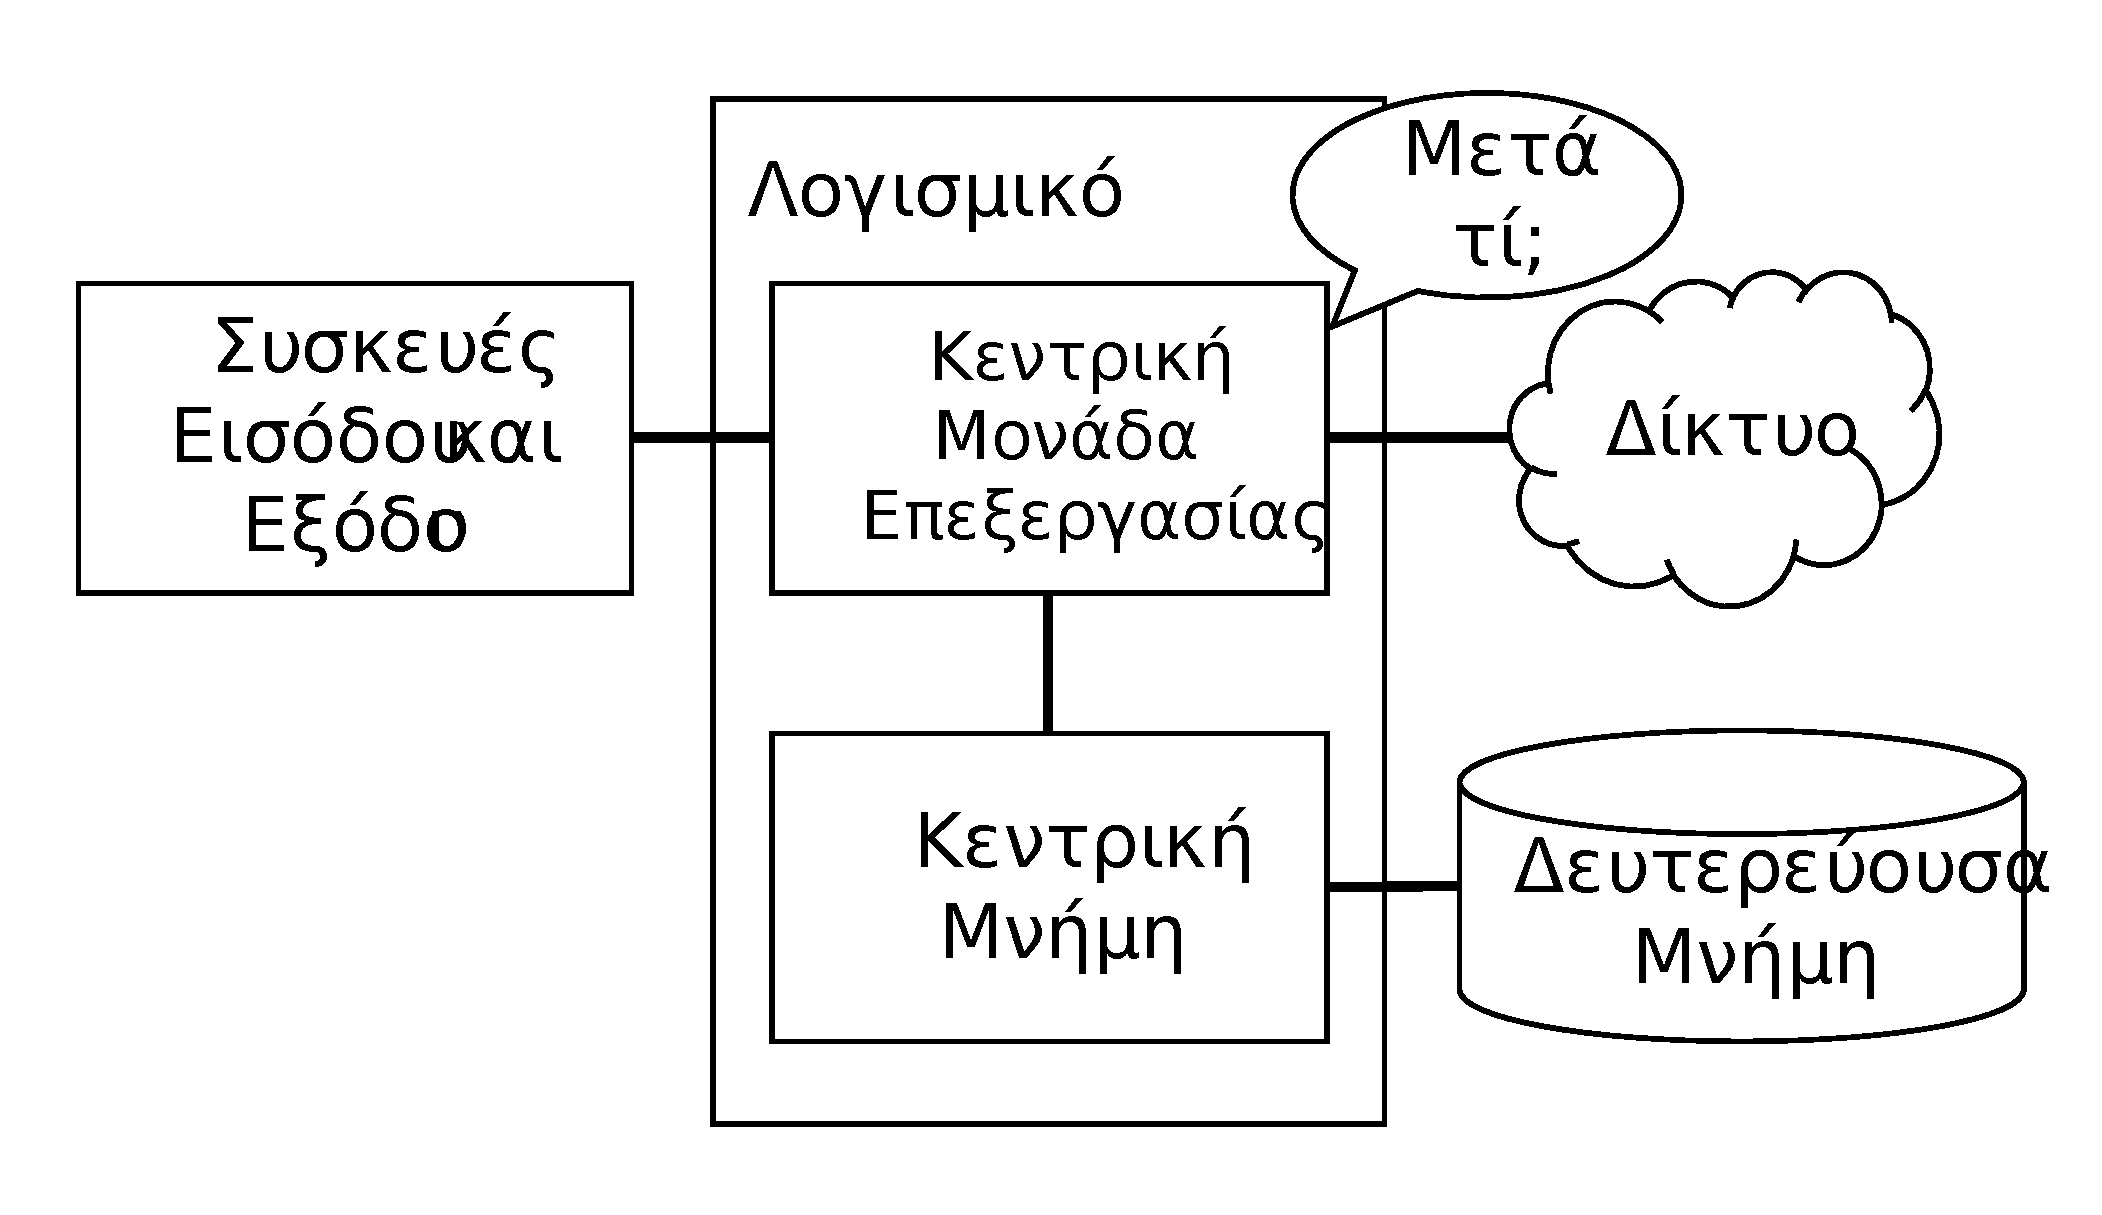
\includegraphics[keepaspectratio,alt={Secondary Memory},height=2.5in]{../images/arch.eps}}
\caption{Secondary Memory}
\end{figure}

Sa chapter na ito, nagsisimula tayong magtrabaho sa \emph{Secondary
Memory} (o files). Ang Secondary memory ay hindi nabubura kapag ang
power ay naka-off. O sa kaso ng USB flash drive, ang data na isinusulat
natin mula sa programs natin ay maaaring alisin sa system at dalhin sa
iba pang system.

Pangunahing tututukan natin ang pagbabasa at pagsusulat ng text files
tulad ng mga ginagawa natin sa text editor. Mamaya makikita natin kung
paano magtrabaho sa database files na binary files, partikular na
idinisenyo para basahin at sulatan sa pamamagitan ng database software.

\section{Opening files}\label{opening-files}

\index{file!open} \index{open function} \index{function!open}

Kapag gusto nating magbasa o sumulat ng file (sabihin sa hard drive mo),
una dapat nating \emph{buksan} ang file. Ang pagbubukas ng file ay
nakikipag-ugnayan sa operating system mo, na alam kung saan naka-store
ang data para sa bawat file. Kapag nagbubukas ka ng file, hinihiling mo
sa operating system na hanapin ang file sa pamamagitan ng pangalan at
siguraduhin na umiiral ang file. Sa halimbawang ito, binubuksan natin
ang file na \emph{mbox.txt}, na dapat naka-store sa parehong folder kung
saan ka kapag nagsimula ka ng Python. Maaari mong i-download ang file na
ito mula sa
\href{http://www.py4e.com/code3/mbox.txt}{www.py4e.com/code3/mbox.txt}

\begin{Shaded}
\begin{Highlighting}[]
\OperatorTok{\textgreater{}\textgreater{}\textgreater{}}\NormalTok{ fhand }\OperatorTok{=} \BuiltInTok{open}\NormalTok{(}\StringTok{\textquotesingle{}mbox.txt\textquotesingle{}}\NormalTok{)}
\OperatorTok{\textgreater{}\textgreater{}\textgreater{}} \BuiltInTok{print}\NormalTok{(fhand)}
\OperatorTok{\textless{}}\NormalTok{\_io.TextIOWrapper name}\OperatorTok{=}\StringTok{\textquotesingle{}mbox.txt\textquotesingle{}}\NormalTok{ mode}\OperatorTok{=}\StringTok{\textquotesingle{}r\textquotesingle{}}\NormalTok{ encoding}\OperatorTok{=}\StringTok{\textquotesingle{}cp1252\textquotesingle{}}\OperatorTok{\textgreater{}}
\end{Highlighting}
\end{Shaded}

\index{file handle}

Kung ang \texttt{open} ay matagumpay, ang operating system ay
nagre-return sa atin ng \emph{file handle}. Ang file handle ay hindi ang
actual data na nasa file, sa halip ito ay ``handle'' na maaari nating
gamitin para basahin ang data. Bibigyan ka ng handle kung ang requested
file ay umiiral at mayroon kang tamang permissions para basahin ang
file.

\begin{figure}
\centering
\pandocbounded{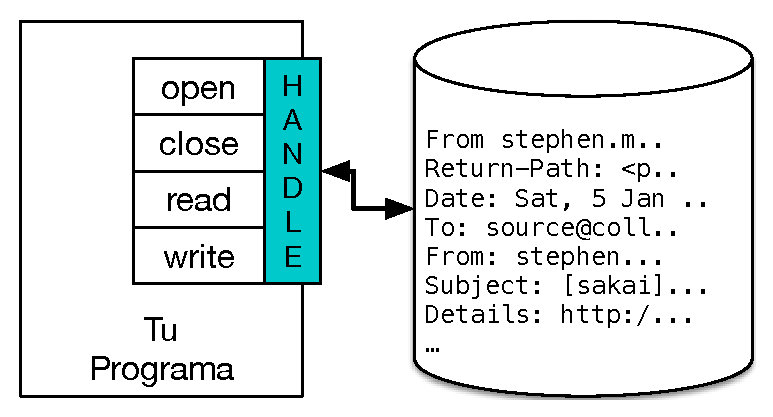
\includegraphics[keepaspectratio,alt={A File Handle},height=2.0in]{../images/handle.eps}}
\caption{A File Handle}
\end{figure}

Kung ang file ay hindi umiiral, ang \texttt{open} ay mabibigo na may
traceback at hindi ka makakakuha ng handle para ma-access ang contents
ng file:

\begin{Shaded}
\begin{Highlighting}[]
\OperatorTok{\textgreater{}\textgreater{}\textgreater{}}\NormalTok{ fhand }\OperatorTok{=} \BuiltInTok{open}\NormalTok{(}\StringTok{\textquotesingle{}stuff.txt\textquotesingle{}}\NormalTok{)}
\NormalTok{Traceback (most recent call last):}
\NormalTok{File }\StringTok{"\textless{}stdin\textgreater{}"}\NormalTok{, line }\DecValTok{1}\NormalTok{, }\KeywordTok{in} \OperatorTok{\textless{}}\NormalTok{module}\OperatorTok{\textgreater{}}
\PreprocessorTok{FileNotFoundError}\NormalTok{: [Errno }\DecValTok{2}\NormalTok{] No such }\BuiltInTok{file} \KeywordTok{or}\NormalTok{ directory: }\StringTok{\textquotesingle{}stuff.txt\textquotesingle{}}
\end{Highlighting}
\end{Shaded}

Mamaya gagamitin natin ang \texttt{try} at \texttt{except} para harapin
nang mas maayos ang situation kung saan sinusubukan nating buksan ang
file na hindi umiiral.

\section{Text files and lines}\label{text-files-and-lines}

Ang text file ay maaaring isipin bilang sequence ng mga linya, katulad
ng Python string na maaaring isipin bilang sequence ng characters.
Halimbawa, ito ay sample ng text file na nagre-record ng mail activity
mula sa iba't ibang indibidwal sa open source project development team:

{\small
\begin{verbatim}
From stephen.marquard@uct.ac.za Sat Jan  5 09:14:16 2008
Return-Path: <postmaster@collab.sakaiproject.org>
Date: Sat, 5 Jan 2008 09:12:18 -0500
To: source@collab.sakaiproject.org
From: stephen.marquard@uct.ac.za
Subject: [sakai] svn commit: r39772 - content/branches/
Details: http://source.sakaiproject.org/viewsvn/?view=rev&rev=39772
...
\end{verbatim}
}

Ang buong file ng mail interactions ay available mula sa

\href{http://www.py4e.com/code3/mbox.txt}{www.py4e.com/code3/mbox.txt}

at ang pinaikling bersyon ng file ay available mula sa

\href{http://www.py4e.com/code3/mbox-short.txt}{www.py4e.com/code3/mbox-short.txt}

Ang mga files na ito ay nasa standard format para sa file na naglalaman
ng maraming mail messages. Ang mga linya na nagsisimula sa ``From'' ay
naghihiwalay ng messages at ang mga linya na nagsisimula sa ``From:'' ay
parte ng messages. Para sa higit pa information tungkol sa mbox format,
tingnan ang \url{https://en.wikipedia.org/wiki/Mbox}.

Para hatiin ang file sa mga linya, mayroong espesyal na character na
kumakatawan sa ``end of the line'' na tinatawag na \emph{newline}
character.

\index{newline}

Sa Python, kinakatawan natin ang \emph{newline} character bilang
backslash-n sa string constants. Kahit na mukhang dalawang characters
ito, ito ay talagang isang character lang. Kapag tinitingnan natin ang
variable sa pamamagitan ng pag-enter ng ``stuff'' sa interpreter,
ipinapakita nito sa atin ang \texttt{\textbackslash{}n} sa string, pero
kapag ginagamit natin ang \texttt{print} para ipakita ang string,
nakikita natin ang string na nahati sa dalawang linya ng newline
character.

\begin{Shaded}
\begin{Highlighting}[]
\OperatorTok{\textgreater{}\textgreater{}\textgreater{}}\NormalTok{ stuff }\OperatorTok{=} \StringTok{\textquotesingle{}Hello}\CharTok{\textbackslash{}n}\StringTok{World!\textquotesingle{}}
\OperatorTok{\textgreater{}\textgreater{}\textgreater{}}\NormalTok{ stuff}
\CommentTok{\textquotesingle{}Hello}\CharTok{\textbackslash{}n}\CommentTok{World!\textquotesingle{}}
\OperatorTok{\textgreater{}\textgreater{}\textgreater{}} \BuiltInTok{print}\NormalTok{(stuff)}
\NormalTok{Hello}
\NormalTok{World}\OperatorTok{!}
\OperatorTok{\textgreater{}\textgreater{}\textgreater{}}\NormalTok{ stuff }\OperatorTok{=} \StringTok{\textquotesingle{}X}\CharTok{\textbackslash{}n}\StringTok{Y\textquotesingle{}}
\OperatorTok{\textgreater{}\textgreater{}\textgreater{}} \BuiltInTok{print}\NormalTok{(stuff)}
\NormalTok{X}
\NormalTok{Y}
\OperatorTok{\textgreater{}\textgreater{}\textgreater{}} \BuiltInTok{len}\NormalTok{(stuff)}
\DecValTok{3}
\end{Highlighting}
\end{Shaded}

Makikita mo rin na ang haba ng string na \texttt{X\textbackslash{}nY} ay
\emph{tatlo} characters dahil ang newline character ay isang character
lang.

Kaya kapag tinitingnan natin ang mga linya sa file, kailangan nating
\emph{isipin} na mayroong espesyal na invisible character na tinatawag
na newline sa dulo ng bawat linya na nagma-marka ng dulo ng linya.

Kaya ang newline character ay naghihiwalay ng characters sa file sa mga
linya.

\section{Reading files}\label{reading-files}

\index{file!reading} \index{counter}

Habang ang \emph{file handle} ay hindi naglalaman ng data para sa file,
napakadaling gumawa ng \texttt{for} loop para magbasa at bilangin ang
bawat linya sa file:

\begin{Shaded}
\begin{Highlighting}[]
\NormalTok{fhand }\OperatorTok{=} \BuiltInTok{open}\NormalTok{(}\StringTok{\textquotesingle{}mbox{-}short.txt\textquotesingle{}}\NormalTok{)}
\NormalTok{count }\OperatorTok{=} \DecValTok{0}
\ControlFlowTok{for}\NormalTok{ line }\KeywordTok{in}\NormalTok{ fhand:}
\NormalTok{    count }\OperatorTok{=}\NormalTok{ count }\OperatorTok{+} \DecValTok{1}
\BuiltInTok{print}\NormalTok{(}\StringTok{\textquotesingle{}Line Count:\textquotesingle{}}\NormalTok{, count)}

\CommentTok{\# Code: https://www.py4e.com/code3/open.py}
\end{Highlighting}
\end{Shaded}

\begin{trinketfiles}
../code3/mbox-short.txt
\end{trinketfiles}

Maaari nating gamitin ang file handle bilang sequence sa \texttt{for}
loop natin. Ang \texttt{for} loop natin ay simpleng nagbi-bilang ng
bilang ng lines sa file at nagpi-print sa kanila. Ang rough translation
ng \texttt{for} loop sa English ay, ``para sa bawat linya sa file na
kinakatawan ng file handle, magdagdag ng isa sa variable na
\texttt{count}.''

Ang dahilan na ang \texttt{open} function ay hindi nagbabasa ng buong
file ay maaaring napakalaki ang file na may maraming gigabytes ng data.
Ang \texttt{open} statement ay tumatagal ng parehong dami ng panahon
anuman ang laki ng file. Ang \texttt{for} loop talaga ang nagdudulot na
ang data ay mabasa mula sa file.

Kapag ang file ay binabasa gamit ang \texttt{for} loop sa ganitong
paraan, ang Python ay nag-aalaga sa paghahati ng data sa file sa hiwalay
na mga linya gamit ang newline character. Ang Python ay nagbabasa ng
bawat linya hanggang sa newline at kasama ang newline bilang huling
character sa variable na \texttt{line} para sa bawat iteration ng
\texttt{for} loop.

Dahil ang \texttt{for} loop ay nagbabasa ng data isang linya sa isang
panahon, maaari itong mabisa na magbasa at magbilang ng mga linya sa
napakalaking files nang hindi naubusan ng main memory para i-store ang
data. Ang program sa itaas ay maaaring magbilang ng mga linya sa anumang
laking file gamit ang napakakaunting memory dahil ang bawat linya ay
binabasa, binibilang, at pagkatapos itinatapon.

Kung alam mo na ang file ay medyo maliit kumpara sa laki ng iyong main
memory, maaari mong basahin ang buong file sa isang string gamit ang
\texttt{read} method sa file handle.

\begin{Shaded}
\begin{Highlighting}[]
\OperatorTok{\textgreater{}\textgreater{}\textgreater{}}\NormalTok{ fhand }\OperatorTok{=} \BuiltInTok{open}\NormalTok{(}\StringTok{\textquotesingle{}mbox{-}short.txt\textquotesingle{}}\NormalTok{)}
\OperatorTok{\textgreater{}\textgreater{}\textgreater{}}\NormalTok{ inp }\OperatorTok{=}\NormalTok{ fhand.read()}
\OperatorTok{\textgreater{}\textgreater{}\textgreater{}} \BuiltInTok{print}\NormalTok{(}\BuiltInTok{len}\NormalTok{(inp))}
\DecValTok{94626}
\OperatorTok{\textgreater{}\textgreater{}\textgreater{}} \BuiltInTok{print}\NormalTok{(inp[:}\DecValTok{20}\NormalTok{])}
\NormalTok{From stephen.marquar}
\end{Highlighting}
\end{Shaded}

Sa halimbawang ito, ang buong contents (lahat ng 94,626 characters) ng
file \emph{mbox-short.txt} ay direktang binabasa sa variable na
\texttt{inp}. Ginagamit natin ang string slicing para i-print ang unang
20 characters ng string data na naka-store sa \texttt{inp}.

Kapag ang file ay binabasa sa ganitong paraan, lahat ng characters
kasama ang lahat ng mga linya at newline characters ay isang malaking
string sa variable na \texttt{inp}. Magandang ideya na i-store ang
output ng \texttt{read} bilang variable dahil ang bawat tawag sa
\texttt{read} ay nauubos ang resource:

\begin{Shaded}
\begin{Highlighting}[]
\OperatorTok{\textgreater{}\textgreater{}\textgreater{}}\NormalTok{ fhand }\OperatorTok{=} \BuiltInTok{open}\NormalTok{(}\StringTok{\textquotesingle{}mbox{-}short.txt\textquotesingle{}}\NormalTok{)}
\OperatorTok{\textgreater{}\textgreater{}\textgreater{}} \BuiltInTok{print}\NormalTok{(}\BuiltInTok{len}\NormalTok{(fhand.read()))}
\DecValTok{94626}
\OperatorTok{\textgreater{}\textgreater{}\textgreater{}} \BuiltInTok{print}\NormalTok{(}\BuiltInTok{len}\NormalTok{(fhand.read()))}
\DecValTok{0}
\end{Highlighting}
\end{Shaded}

Tandaan na ang form ng \texttt{open} function na ito ay dapat lang
gamitin kung ang file data ay magkakasya nang komportable sa main memory
ng computer mo. Kung ang file ay masyadong malaki para magkasya sa main
memory, dapat mong isulat ang program mo para basahin ang file sa chunks
gamit ang \texttt{for} o \texttt{while} loop.

\section{Searching through a file}\label{searching-through-a-file}

Kapag naghahanap ka sa data sa file, napakakaraniwang pattern na magbasa
sa file, hindi pinapansin ang karamihan ng mga linya at nagpo-process
lang ng mga linya na tumutugma sa partikular na condition. Maaari nating
pagsamahin ang pattern para magbasa ng file kasama ang string methods
para gumawa ng simpleng search mechanisms.

\index{filter pattern} \index{pattern!filter}

Halimbawa, kung gusto nating magbasa ng file at mag-print lang ng mga
linya na nagsimula sa prefix na ``From:'', maaari nating gamitin ang
string method na \emph{startswith} para pumili lang ng mga linya na may
gustong prefix:

\begin{Shaded}
\begin{Highlighting}[]
\NormalTok{fhand }\OperatorTok{=} \BuiltInTok{open}\NormalTok{(}\StringTok{\textquotesingle{}mbox{-}short.txt\textquotesingle{}}\NormalTok{)}
\ControlFlowTok{for}\NormalTok{ line }\KeywordTok{in}\NormalTok{ fhand:}
    \ControlFlowTok{if}\NormalTok{ line.startswith(}\StringTok{\textquotesingle{}From:\textquotesingle{}}\NormalTok{):}
        \BuiltInTok{print}\NormalTok{(line)}

\CommentTok{\# Code: https://www.py4e.com/code3/search1.py}
\end{Highlighting}
\end{Shaded}

\begin{trinketfiles}
../code3/mbox-short.txt
\end{trinketfiles}

Kapag tumatakbo ang program na ito, nakakakuha tayo ng sumusunod na
output:

{\small
\begin{verbatim}
From: stephen.marquard@uct.ac.za

From: louis@media.berkeley.edu

From: zqian@umich.edu

From: rjlowe@iupui.edu
...
\end{verbatim}
}

Ang output ay mukhang maganda dahil ang tanging mga linya na nakikita
natin ay ang mga nagsisimula sa ``From:'', pero bakit nakikita natin ang
extra blank lines? Ito ay dahil sa invisible na \emph{newline} character
na iyon. Ang bawat isa sa mga linya ay nagtatapos sa newline, kaya ang
\texttt{print} statement ay nagpi-print ng string sa variable na
\emph{line} na kasama ang newline at pagkatapos ang \texttt{print} ay
nagdadagdag ng \emph{isa pa} na newline, na nagreresulta sa double
spacing effect na nakikita natin.

Maaari nating gamitin ang line slicing para i-print ang lahat maliban sa
huling character, pero ang mas simpleng approach ay gamitin ang
\emph{rstrip} method na nagtatanggal ng whitespaces mula sa kanang
bahagi ng string tulad ng sumusunod:

\begin{Shaded}
\begin{Highlighting}[]
\NormalTok{fhand }\OperatorTok{=} \BuiltInTok{open}\NormalTok{(}\StringTok{\textquotesingle{}mbox{-}short.txt\textquotesingle{}}\NormalTok{)}
\ControlFlowTok{for}\NormalTok{ line }\KeywordTok{in}\NormalTok{ fhand:}
\NormalTok{    line }\OperatorTok{=}\NormalTok{ line.rstrip()}
    \ControlFlowTok{if}\NormalTok{ line.startswith(}\StringTok{\textquotesingle{}From:\textquotesingle{}}\NormalTok{):}
        \BuiltInTok{print}\NormalTok{(line)}

\CommentTok{\# Code: https://www.py4e.com/code3/search2.py}
\end{Highlighting}
\end{Shaded}

\begin{trinketfiles}
../code3/mbox-short.txt
\end{trinketfiles}

Kapag tumatakbo ang program na ito, nakakakuha tayo ng sumusunod na
output:

{\small
\begin{verbatim}
From: stephen.marquard@uct.ac.za
From: louis@media.berkeley.edu
From: zqian@umich.edu
From: rjlowe@iupui.edu
From: zqian@umich.edu
From: rjlowe@iupui.edu
From: cwen@iupui.edu
...
\end{verbatim}
}

Habang ang file processing programs mo ay nagiging mas kumplikado,
maaaring gusto mong i-structure ang search loops mo gamit ang
\texttt{continue}. Ang basic idea ng search loop ay naghahanap ka ng
``interesting'' lines at epektibong nilalaktawan ang ``uninteresting''
lines. At pagkatapos kapag nakakita tayo ng interesting line, gumagawa
tayo ng isang bagay sa linya na iyon.

Maaari nating i-structure ang loop para sundin ang pattern ng paglaktaw
sa uninteresting lines tulad ng sumusunod:

\begin{Shaded}
\begin{Highlighting}[]
\NormalTok{fhand }\OperatorTok{=} \BuiltInTok{open}\NormalTok{(}\StringTok{\textquotesingle{}mbox{-}short.txt\textquotesingle{}}\NormalTok{)}
\ControlFlowTok{for}\NormalTok{ line }\KeywordTok{in}\NormalTok{ fhand:}
\NormalTok{    line }\OperatorTok{=}\NormalTok{ line.rstrip()}
    \CommentTok{\# Skip \textquotesingle{}uninteresting lines\textquotesingle{}}
    \ControlFlowTok{if} \KeywordTok{not}\NormalTok{ line.startswith(}\StringTok{\textquotesingle{}From:\textquotesingle{}}\NormalTok{):}
        \ControlFlowTok{continue}
    \CommentTok{\# Process our \textquotesingle{}interesting\textquotesingle{} line}
    \BuiltInTok{print}\NormalTok{(line)}

\CommentTok{\# Code: https://www.py4e.com/code3/search3.py}
\end{Highlighting}
\end{Shaded}

\begin{trinketfiles}
../code3/mbox-short.txt
\end{trinketfiles}

Ang output ng program ay pareho. Sa English, ang uninteresting lines ay
ang mga hindi nagsisimula sa ``From:'', na nilalaktawan natin gamit ang
\texttt{continue}. Para sa ``interesting'' lines (i.e., ang mga
nagsisimula sa ``From:'') ginagawa natin ang processing.

Maaari nating gamitin ang \texttt{find} string method para gayahin ang
text editor search na nakakahanap ng mga linya kung saan ang search
string ay nasa kahit saan sa linya. Dahil ang \texttt{find} ay
naghahanap ng occurrence ng string sa loob ng ibang string at
nagre-return ng posisyon ng string o -1 kung hindi nahanap ang string,
maaari tayong sumulat ng sumusunod na loop para ipakita ang mga linya na
naglalaman ng string na ``@uct.ac.za'' (i.e., galing sila sa University
of Cape Town sa South Africa):

\begin{Shaded}
\begin{Highlighting}[]
\NormalTok{fhand }\OperatorTok{=} \BuiltInTok{open}\NormalTok{(}\StringTok{\textquotesingle{}mbox{-}short.txt\textquotesingle{}}\NormalTok{)}
\ControlFlowTok{for}\NormalTok{ line }\KeywordTok{in}\NormalTok{ fhand:}
\NormalTok{    line }\OperatorTok{=}\NormalTok{ line.rstrip()}
    \ControlFlowTok{if}\NormalTok{ line.find(}\StringTok{\textquotesingle{}@uct.ac.za\textquotesingle{}}\NormalTok{) }\OperatorTok{==} \OperatorTok{{-}}\DecValTok{1}\NormalTok{: }\ControlFlowTok{continue}
    \BuiltInTok{print}\NormalTok{(line)}

\CommentTok{\# Code: https://www.py4e.com/code3/search4.py}
\end{Highlighting}
\end{Shaded}

\begin{trinketfiles}
../code3/mbox-short.txt
\end{trinketfiles}

Na gumagawa ng sumusunod na output:

{\small
\begin{verbatim}
From stephen.marquard@uct.ac.za Sat Jan  5 09:14:16 2008
X-Authentication-Warning: set sender to stephen.marquard@uct.ac.za using -f
From: stephen.marquard@uct.ac.za
Author: stephen.marquard@uct.ac.za
From david.horwitz@uct.ac.za Fri Jan  4 07:02:32 2008
X-Authentication-Warning: set sender to david.horwitz@uct.ac.za using -f
From: david.horwitz@uct.ac.za
Author: david.horwitz@uct.ac.za
...
\end{verbatim}
}

Dito ginagamit din natin ang contracted form ng \texttt{if} statement
kung saan inilalagay natin ang \texttt{continue} sa parehong linya ng
\texttt{if}. Ang contracted form ng \texttt{if} na ito ay gumagana
pareho kung ang \texttt{continue} ay nasa susunod na linya at
naka-indent.

\section{Letting the user choose the file
name}\label{letting-the-user-choose-the-file-name}

Talagang ayaw nating kailanganin na i-edit ang Python code natin sa
bawat pagkakataon na gusto nating i-process ang ibang file. Mas magiging
magagamit kung hihilingin natin sa user na mag-enter ng file name string
sa bawat pagkakataon na tumatakbo ang program para magamit nila ang
program natin sa iba't ibang files nang hindi binabago ang Python code.

Napakasimple gawin ito sa pamamagitan ng pagbasa ng file name mula sa
user gamit ang \texttt{input} tulad ng sumusunod:

\begin{Shaded}
\begin{Highlighting}[]
\NormalTok{fname }\OperatorTok{=} \BuiltInTok{input}\NormalTok{(}\StringTok{\textquotesingle{}Enter the file name: \textquotesingle{}}\NormalTok{)}
\NormalTok{fhand }\OperatorTok{=} \BuiltInTok{open}\NormalTok{(fname)}
\NormalTok{count }\OperatorTok{=} \DecValTok{0}
\ControlFlowTok{for}\NormalTok{ line }\KeywordTok{in}\NormalTok{ fhand:}
    \ControlFlowTok{if}\NormalTok{ line.startswith(}\StringTok{\textquotesingle{}Subject:\textquotesingle{}}\NormalTok{):}
\NormalTok{        count }\OperatorTok{=}\NormalTok{ count }\OperatorTok{+} \DecValTok{1}
\BuiltInTok{print}\NormalTok{(}\StringTok{\textquotesingle{}There were\textquotesingle{}}\NormalTok{, count, }\StringTok{\textquotesingle{}subject lines in\textquotesingle{}}\NormalTok{, fname)}

\CommentTok{\# Code: https://www.py4e.com/code3/search6.py}
\end{Highlighting}
\end{Shaded}

\begin{trinketfiles}
../code3/mbox-short.txt
\end{trinketfiles}

Binabasa natin ang file name mula sa user at inilalagay ito sa variable
na may pangalang \texttt{fname} at binubuksan ang file na iyon. Ngayon
maaari na nating patakbuhin ang program nang paulit-ulit sa iba't ibang
files.

{\small
\begin{verbatim}
python search6.py
Enter the file name: mbox.txt
There were 1797 subject lines in mbox.txt

python search6.py
Enter the file name: mbox-short.txt
There were 27 subject lines in mbox-short.txt
\end{verbatim}
}

Bago tumingin sa susunod na section, tingnan ang program sa itaas at
tanungin ang sarili mo, ``Ano ang maaaring maging mali dito?'' o ``Ano
ang maaaring gawin ng friendly user natin na magdudulot na ang nice
little program natin ay lumabas nang hindi maayos na may traceback, na
ginagawang hindi masyadong cool tayo sa mga mata ng users natin?''

\section{\texorpdfstring{Using \texttt{try,\ except,} and
\texttt{open}}{Using try, except, and open}}\label{using-try-except-and-open}

Sinabi ko sa iyo na huwag tumingin. Ito na ang huling pagkakataon mo.

Paano kung ang user natin ay nagta-type ng isang bagay na hindi file
name?

{\small
\begin{verbatim}
python search6.py
Enter the file name: missing.txt
Traceback (most recent call last):
  File "search6.py", line 2, in <module>
    fhand = open(fname)
FileNotFoundError: [Errno 2] No such file or directory: 'missing.txt'

python search6.py
Enter the file name: na na boo boo
Traceback (most recent call last):
  File "search6.py", line 2, in <module>
    fhand = open(fname)
FileNotFoundError: [Errno 2] No such file or directory: 'na na boo boo'
\end{verbatim}
}

Huwag tumawa. Ang mga users ay sa huli ay gagawin ang bawat posibleng
bagay na magagawa nila para sirain ang programs mo, maaaring hindi
sinasadya o may masamang layunin. Bilang matter of fact, mahalagang
parte ng anumang software development team ay isang tao o grupo na
tinatawag na \emph{Quality Assurance} (o QA para sa maikli) na ang
trabaho ay gawin ang pinakamabaliw na bagay na posible sa pagtatangka na
sirain ang software na ginawa ng programmer.

\index{Quality Assurance} \index{QA}

Ang QA team ay responsable sa paghahanap ng flaws sa programs bago natin
nai-deliver ang program sa end users na maaaring bumibili ng software o
nagbabayad ng suweldo natin para sumulat ng software. Kaya ang QA team
ay pinakamabuting kaibigan ng programmer.

\index{try statement} \index{statement!try} \index{open function}
\index{function!open} \index{exception!IOError} \index{IOError}

Kaya ngayon na nakikita natin ang flaw sa program, maaari nating maayos
na ayusin ito gamit ang \texttt{try}/\texttt{except} structure.
Kailangan nating i-assume na ang \texttt{open} call ay maaaring mabigo
at magdagdag ng recovery code kapag ang \texttt{open} ay nabigo tulad ng
sumusunod:

\begin{Shaded}
\begin{Highlighting}[]
\NormalTok{fname }\OperatorTok{=} \BuiltInTok{input}\NormalTok{(}\StringTok{\textquotesingle{}Enter the file name: \textquotesingle{}}\NormalTok{)}
\ControlFlowTok{try}\NormalTok{:}
\NormalTok{    fhand }\OperatorTok{=} \BuiltInTok{open}\NormalTok{(fname)}
\ControlFlowTok{except}\NormalTok{:}
    \BuiltInTok{print}\NormalTok{(}\StringTok{\textquotesingle{}File cannot be opened:\textquotesingle{}}\NormalTok{, fname)}
\NormalTok{    exit()}
\NormalTok{count }\OperatorTok{=} \DecValTok{0}
\ControlFlowTok{for}\NormalTok{ line }\KeywordTok{in}\NormalTok{ fhand:}
    \ControlFlowTok{if}\NormalTok{ line.startswith(}\StringTok{\textquotesingle{}Subject:\textquotesingle{}}\NormalTok{):}
\NormalTok{        count }\OperatorTok{=}\NormalTok{ count }\OperatorTok{+} \DecValTok{1}
\BuiltInTok{print}\NormalTok{(}\StringTok{\textquotesingle{}There were\textquotesingle{}}\NormalTok{, count, }\StringTok{\textquotesingle{}subject lines in\textquotesingle{}}\NormalTok{, fname)}

\CommentTok{\# Code: https://www.py4e.com/code3/search7.py}
\end{Highlighting}
\end{Shaded}

\begin{trinketfiles}
../code3/mbox-short.txt
\end{trinketfiles}

Ang \texttt{exit} function ay nagtatapos ng program. Ito ay function na
tinatawag natin na hindi kailanman nagre-return. Ngayon kapag ang user
natin (o QA team) ay nagta-type ng kalokohan o masamang file names,
``hinuhuli'' natin sila at nagre-recover nang maayos:

{\small
\begin{verbatim}
python search7.py
Enter the file name: mbox.txt
There were 1797 subject lines in mbox.txt

python search7.py
Enter the file name: na na boo boo
File cannot be opened: na na boo boo
\end{verbatim}
}

\index{Pythonic}

Ang pagprotekta sa \texttt{open} call ay magandang halimbawa ng tamang
paggamit ng \texttt{try} at \texttt{except} sa Python program. Ginagamit
natin ang term na ``Pythonic'' kapag gumagawa tayo ng isang bagay sa
``Python way''. Maaari nating sabihin na ang halimbawa sa itaas ay ang
Pythonic way para buksan ang file.

Kapag naging mas bihasa ka na sa Python, maaari kang makipag-repartee sa
iba pang Python programmers para magpasya kung alin sa dalawang katumbas
na solusyon sa problema ang ``mas Pythonic''. Ang layunin na maging
``mas Pythonic'' ay kumukuha ng konsepto na ang programming ay parte
engineering at parte art. Hindi tayo palaging interesado lang na gumawa
ng isang bagay na gumagana, gusto din natin na ang solusyon natin ay
elegant at maa-appreciate bilang elegant ng mga kapantay natin.

\section{Writing files}\label{writing-files}

\index{file!writing}

Para sumulat ng file, kailangan mong buksan ito na may mode na ``w''
bilang pangalawang parameter:

\begin{Shaded}
\begin{Highlighting}[]
\OperatorTok{\textgreater{}\textgreater{}\textgreater{}}\NormalTok{ fout }\OperatorTok{=} \BuiltInTok{open}\NormalTok{(}\StringTok{\textquotesingle{}output.txt\textquotesingle{}}\NormalTok{, }\StringTok{\textquotesingle{}w\textquotesingle{}}\NormalTok{)}
\OperatorTok{\textgreater{}\textgreater{}\textgreater{}} \BuiltInTok{print}\NormalTok{(fout)}
\OperatorTok{\textless{}}\NormalTok{\_io.TextIOWrapper name}\OperatorTok{=}\StringTok{\textquotesingle{}output.txt\textquotesingle{}}\NormalTok{ mode}\OperatorTok{=}\StringTok{\textquotesingle{}w\textquotesingle{}}\NormalTok{ encoding}\OperatorTok{=}\StringTok{\textquotesingle{}cp1252\textquotesingle{}}\OperatorTok{\textgreater{}}
\end{Highlighting}
\end{Shaded}

Kung ang file ay umiiral na, ang pagbubukas nito sa write mode ay
naglilinis ng lumang data at nagsisimula ng fresh, kaya mag-ingat! Kung
ang file ay hindi umiiral, bago ang gagawin.

Ang \texttt{write} method ng file handle object ay naglalagay ng data sa
file, na nagre-return ng bilang ng characters na naisulat. Ang default
write mode ay text para sa pagsusulat (at pagbabasa) ng strings.

\begin{Shaded}
\begin{Highlighting}[]
\OperatorTok{\textgreater{}\textgreater{}\textgreater{}}\NormalTok{ line1 }\OperatorTok{=} \StringTok{"This here\textquotesingle{}s the wattle,}\CharTok{\textbackslash{}n}\StringTok{"}
\OperatorTok{\textgreater{}\textgreater{}\textgreater{}}\NormalTok{ fout.write(line1)}
\DecValTok{24}
\end{Highlighting}
\end{Shaded}

\index{newline}

Muli, ang file object ay nagsu-subaybay kung nasaan ito, kaya kung
tatawagin mo ang \texttt{write} ulit, idinadagdag nito ang bagong data
sa dulo.

Dapat nating siguraduhin na pamahalaan ang dulo ng mga linya habang
sumusulat tayo sa file sa pamamagitan ng tahasang paglalagay ng newline
character kapag gusto nating tapusin ang linya. Ang \texttt{print}
statement ay awtomatikong nag-a-append ng newline, pero ang
\texttt{write} method ay hindi nagdadagdag ng newline nang awtomatiko.

\begin{Shaded}
\begin{Highlighting}[]
\OperatorTok{\textgreater{}\textgreater{}\textgreater{}}\NormalTok{ line2 }\OperatorTok{=} \StringTok{\textquotesingle{}the emblem of our land.}\CharTok{\textbackslash{}n}\StringTok{\textquotesingle{}}
\OperatorTok{\textgreater{}\textgreater{}\textgreater{}}\NormalTok{ fout.write(line2)}
\DecValTok{24}
\end{Highlighting}
\end{Shaded}

Kapag tapos ka na sa pagsusulat, kailangan mong isara ang file para
masiguro na ang huling piraso ng data ay pisikal na naisulat sa disk
para hindi ito mawala kung ang power ay mawawala.

\begin{Shaded}
\begin{Highlighting}[]
\OperatorTok{\textgreater{}\textgreater{}\textgreater{}}\NormalTok{ fout.close()}
\end{Highlighting}
\end{Shaded}

Maaari nating isara ang mga files na binubuksan natin para sa pagbabasa
din, pero maaari tayong maging medyo pabaya kung nagbubukas lang tayo ng
ilang files dahil sinisiguro ng Python na lahat ng bukas na files ay
nagsasara kapag natatapos ang program. Kapag sumusulat tayo ng files,
gusto nating tahasang isara ang files para walang maiwan sa pagkakataon.

\index{close method} \index{method!close}

\section{Debugging}\label{debugging-6}

\index{debugging} \index{whitespace}

Kapag nagbabasa at sumusulat ka ng files, maaari kang makatagpo ng mga
problema sa whitespace. Ang mga errors na ito ay maaaring mahirap
i-debug dahil ang spaces, tabs, at newlines ay karaniwang invisible:

\begin{Shaded}
\begin{Highlighting}[]
\OperatorTok{\textgreater{}\textgreater{}\textgreater{}}\NormalTok{ s }\OperatorTok{=} \StringTok{\textquotesingle{}1 2}\CharTok{\textbackslash{}t}\StringTok{ 3}\CharTok{\textbackslash{}n}\StringTok{ 4\textquotesingle{}}
\OperatorTok{\textgreater{}\textgreater{}\textgreater{}} \BuiltInTok{print}\NormalTok{(s)}
\DecValTok{1} \DecValTok{2}  \DecValTok{3}
 \DecValTok{4}
\end{Highlighting}
\end{Shaded}

\index{repr function} \index{function!repr}
\index{string representation}

Ang built-in function na \texttt{repr} ay maaaring makatulong.
Tumatanggap ito ng anumang object bilang argument at nagre-return ng
string representation ng object. Para sa strings, kinakatawan nito ang
whitespace characters gamit ang backslash sequences:

\begin{Shaded}
\begin{Highlighting}[]
\OperatorTok{\textgreater{}\textgreater{}\textgreater{}} \BuiltInTok{print}\NormalTok{(}\BuiltInTok{repr}\NormalTok{(s))}
\CommentTok{\textquotesingle{}1 2}\CharTok{\textbackslash{}t}\CommentTok{ 3}\CharTok{\textbackslash{}n}\CommentTok{ 4\textquotesingle{}}
\end{Highlighting}
\end{Shaded}

Ito ay maaaring makatulong para sa debugging.

Ang isa pang problema na maaaring makatagpo ka ay ang iba't ibang
systems ay gumagamit ng iba't ibang characters para ipahiwatig ang dulo
ng linya. Ang ilang systems ay gumagamit ng newline, na kinakatawan ng
\texttt{\textbackslash{}n}. Ang iba ay gumagamit ng return character, na
kinakatawan ng \texttt{\textbackslash{}r}. Ang ilan ay gumagamit ng
pareho. Kung ililipat mo ang files sa pagitan ng iba't ibang systems,
ang mga inconsistencies na ito ay maaaring magdulot ng mga problema.

\index{end of line character}

Para sa karamihan ng systems, mayroong applications para i-convert mula
sa isang format patungo sa iba. Maaari mong hanapin ang mga ito (at
magbasa pa tungkol sa issue na ito) sa
\href{https://wikipedia.org/wiki/Newline}{https://www.wikipedia.org/wiki/Newline}.
O, siyempre, maaari mong isulat ang isa sa iyong sarili.

\section{Glossary}\label{glossary-6}

\begin{description}
\tightlist
\item[catch]
Para pigilan ang exception na tapusin ang program gamit ang \texttt{try}
at \texttt{except} statements. \index{catch}
\item[newline]
Espesyal na character na ginagamit sa files at strings para ipahiwatig
ang dulo ng linya. \index{newline}
\item[Pythonic]
Technique na gumagana nang elegant sa Python. ``Ang paggamit ng try at
except ay ang \emph{Pythonic} way para makabawi mula sa missing files''.
\index{Pythonic}
\item[Quality Assurance]
Tao o team na nakatuon sa pagtiyak ng overall quality ng software
product. Ang QA ay kadalasang kasangkot sa pag-test ng product at
pagkilala ng mga problema bago i-release ang product.
\index{Quality Assurance} \index{QA}
\item[text file]
Sequence ng characters na naka-store sa permanent storage tulad ng hard
drive. \index{text file}
\end{description}

\section{Exercises}\label{exercises-6}

\textbf{Exercise 1:} Sumulat ng program para magbasa sa file at
mag-print ng contents ng file (linya sa linya) lahat sa upper case. Ang
pag-e-execute ng program ay magiging ganito:

{\small
\begin{verbatim}
python shout.py
Enter a file name: mbox-short.txt
FROM STEPHEN.MARQUARD@UCT.AC.ZA SAT JAN  5 09:14:16 2008
RETURN-PATH: <POSTMASTER@COLLAB.SAKAIPROJECT.ORG>
RECEIVED: FROM MURDER (MAIL.UMICH.EDU [141.211.14.90])
     BY FRANKENSTEIN.MAIL.UMICH.EDU (CYRUS V2.3.8) WITH LMTPA;
     SAT, 05 JAN 2008 09:14:16 -0500
\end{verbatim}
}

Maaari mong i-download ang file mula sa
\href{http://www.py4e.com/code3/mbox-short.txt}{www.py4e.com/code3/mbox-short.txt}

\textbf{Exercise 2:} Sumulat ng program para mag-prompt para sa file
name, at pagkatapos magbasa sa file at maghanap ng mga linya ng form:

{\small
\begin{verbatim}
X-DSPAM-Confidence: 0.8475
\end{verbatim}
}

Kapag nakatagpo ka ng linya na nagsisimula sa ``X-DSPAM-Confidence:''
hatiin ang linya para kunin ang floating-point number sa linya. Bilangin
ang mga linyang ito at pagkatapos i-compute ang kabuuan ng spam
confidence values mula sa mga linyang ito. Kapag naabot mo na ang dulo
ng file, mag-print ng average spam confidence.

{\small
\begin{verbatim}
Enter the file name: mbox.txt
Average spam confidence: 0.894128046745

Enter the file name: mbox-short.txt
Average spam confidence: 0.750718518519
\end{verbatim}
}

I-test ang file mo sa \emph{mbox.txt} at \emph{mbox-short.txt} files.

\textbf{Exercise 3:}

Minsan kapag ang mga programmers ay naiinip o gusto ng kaunting
kasiyahan, nagdadagdag sila ng harmless na \emph{Easter Egg} sa program
nila. Baguhin ang program na nagpo-prompt sa user para sa file name para
mag-print ng nakakatawang mensahe kapag ang user ay nagta-type ng
eksaktong file name na ``na na boo boo''. Ang program ay dapat kumilos
nang normal para sa lahat ng iba pang files na umiiral at hindi umiiral.
Narito ang sample execution ng program:

{\small
\begin{verbatim}
python egg.py
Enter the file name: mbox.txt
There were 1797 subject lines in mbox.txt

python egg.py
Enter the file name: missing.tyxt
File cannot be opened: missing.tyxt

python egg.py
Enter the file name: na na boo boo
NA NA BOO BOO TO YOU - You have been punk'd!
\end{verbatim}
}

Hindi namin hinihikayat na maglagay ng Easter Eggs sa programs mo; ito
ay exercise lang.

\chapter{Lists}\label{lists}

\index{list} \index{type!list}

\section{A list is a sequence}\label{a-list-is-a-sequence}

Tulad ng string, ang \emph{list} ay sequence ng values. Sa string, ang
values ay characters; sa list, maaari silang anumang type. Ang mga
values sa lists ay tinatawag na \emph{elements} o minsan \emph{items}.

\index{element} \index{sequence} \index{item}

Mayroong ilang paraan para gumawa ng bagong list; ang pinakasimple ay
i-enclose ang elements sa square brackets (``{[}'' at ''{]}''):

\begin{Shaded}
\begin{Highlighting}[]
\NormalTok{[}\DecValTok{10}\NormalTok{, }\DecValTok{20}\NormalTok{, }\DecValTok{30}\NormalTok{, }\DecValTok{40}\NormalTok{]}
\NormalTok{[}\StringTok{\textquotesingle{}crunchy frog\textquotesingle{}}\NormalTok{, }\StringTok{\textquotesingle{}ram bladder\textquotesingle{}}\NormalTok{, }\StringTok{\textquotesingle{}lark vomit\textquotesingle{}}\NormalTok{]}
\end{Highlighting}
\end{Shaded}

Ang unang halimbawa ay list ng apat na integers. Ang pangalawa ay list
ng tatlong strings. Ang elements ng list ay hindi kailangang pareho ang
type. Ang sumusunod na list ay naglalaman ng string, float, integer, at
(lo!) isa pang list:

\begin{Shaded}
\begin{Highlighting}[]
\NormalTok{[}\StringTok{\textquotesingle{}spam\textquotesingle{}}\NormalTok{, }\FloatTok{2.0}\NormalTok{, }\DecValTok{5}\NormalTok{, [}\DecValTok{10}\NormalTok{, }\DecValTok{20}\NormalTok{]]}
\end{Highlighting}
\end{Shaded}

Ang list sa loob ng ibang list ay \emph{nested}.

\index{nested list} \index{list!nested}

Ang list na walang elements ay tinatawag na empty list; maaari kang
gumawa ng isa na may empty brackets, \texttt{{[}{]}}.

\index{empty list} \index{list!empty}

Tulad ng maaaring inaasahan mo, maaari mong i-assign ang list values sa
variables:

\begin{Shaded}
\begin{Highlighting}[]
\OperatorTok{\textgreater{}\textgreater{}\textgreater{}}\NormalTok{ cheeses }\OperatorTok{=}\NormalTok{ [}\StringTok{\textquotesingle{}Cheddar\textquotesingle{}}\NormalTok{, }\StringTok{\textquotesingle{}Edam\textquotesingle{}}\NormalTok{, }\StringTok{\textquotesingle{}Gouda\textquotesingle{}}\NormalTok{]}
\OperatorTok{\textgreater{}\textgreater{}\textgreater{}}\NormalTok{ numbers }\OperatorTok{=}\NormalTok{ [}\DecValTok{17}\NormalTok{, }\DecValTok{123}\NormalTok{]}
\OperatorTok{\textgreater{}\textgreater{}\textgreater{}}\NormalTok{ empty }\OperatorTok{=}\NormalTok{ []}
\OperatorTok{\textgreater{}\textgreater{}\textgreater{}} \BuiltInTok{print}\NormalTok{(cheeses, numbers, empty)}
\NormalTok{[}\StringTok{\textquotesingle{}Cheddar\textquotesingle{}}\NormalTok{, }\StringTok{\textquotesingle{}Edam\textquotesingle{}}\NormalTok{, }\StringTok{\textquotesingle{}Gouda\textquotesingle{}}\NormalTok{] [}\DecValTok{17}\NormalTok{, }\DecValTok{123}\NormalTok{] []}
\end{Highlighting}
\end{Shaded}

\index{assignment}

\section{Lists are mutable}\label{lists-are-mutable}

\index{list!element} \index{access} \index{index} \index{}
\index{bracket operator} \index{operator!bracket}

Ang syntax para ma-access ang elements ng list ay pareho sa pag-access
ng characters ng string: ang bracket operator. Ang expression sa loob ng
brackets ay tumutukoy sa index. Tandaan na ang indices ay nagsisimula sa
0:

\begin{Shaded}
\begin{Highlighting}[]
\OperatorTok{\textgreater{}\textgreater{}\textgreater{}} \BuiltInTok{print}\NormalTok{(cheeses[}\DecValTok{0}\NormalTok{])}
\NormalTok{Cheddar}
\end{Highlighting}
\end{Shaded}

Hindi tulad ng strings, ang lists ay mutable dahil maaari mong baguhin
ang order ng items sa list o mag-reassign ng item sa list. Kapag ang
bracket operator ay lumalabas sa kaliwang bahagi ng assignment,
kinikilala nito ang element ng list na ma-a-assign.

\index{mutability}

\begin{Shaded}
\begin{Highlighting}[]
\OperatorTok{\textgreater{}\textgreater{}\textgreater{}}\NormalTok{ numbers }\OperatorTok{=}\NormalTok{ [}\DecValTok{17}\NormalTok{, }\DecValTok{123}\NormalTok{]}
\OperatorTok{\textgreater{}\textgreater{}\textgreater{}}\NormalTok{ numbers[}\DecValTok{1}\NormalTok{] }\OperatorTok{=} \DecValTok{5}
\OperatorTok{\textgreater{}\textgreater{}\textgreater{}} \BuiltInTok{print}\NormalTok{(numbers)}
\NormalTok{[}\DecValTok{17}\NormalTok{, }\DecValTok{5}\NormalTok{]}
\end{Highlighting}
\end{Shaded}

Ang one-th element ng \texttt{numbers}, na dati ay 123, ay ngayon 5.

\index{index!starting at zero} \index{zero, index starting at}

Maaari mong isipin ang list bilang relasyon sa pagitan ng indices at
elements. Ang relasyong ito ay tinatawag na \emph{mapping}; ang bawat
index ay ``nagma-map sa'' isa sa mga elements.

\index{item assignment} \index{assignment!item}

Ang list indices ay gumagana sa parehong paraan ng string indices:

\begin{itemize}
\item
  Anumang integer expression ay maaaring gamitin bilang index.
\item
  Kung susubukan mong basahin o sulatan ang element na hindi umiiral,
  makakakuha ka ng \texttt{IndexError}.
\end{itemize}

\index{exception!IndexError} \index{IndexError}

\begin{itemize}
\tightlist
\item
  Kung ang index ay may negative value, nagbi-bilang ito pabalik mula sa
  dulo ng list.
\end{itemize}

\index{list!index} \index{list!membership} \index{membership!list}
\index{in operator} \index{operator!in}

Ang \texttt{in} operator ay gumagana din sa lists.

\begin{Shaded}
\begin{Highlighting}[]
\OperatorTok{\textgreater{}\textgreater{}\textgreater{}}\NormalTok{ cheeses }\OperatorTok{=}\NormalTok{ [}\StringTok{\textquotesingle{}Cheddar\textquotesingle{}}\NormalTok{, }\StringTok{\textquotesingle{}Edam\textquotesingle{}}\NormalTok{, }\StringTok{\textquotesingle{}Gouda\textquotesingle{}}\NormalTok{]}
\OperatorTok{\textgreater{}\textgreater{}\textgreater{}} \StringTok{\textquotesingle{}Edam\textquotesingle{}} \KeywordTok{in}\NormalTok{ cheeses}
\VariableTok{True}
\OperatorTok{\textgreater{}\textgreater{}\textgreater{}} \StringTok{\textquotesingle{}Brie\textquotesingle{}} \KeywordTok{in}\NormalTok{ cheeses}
\VariableTok{False}
\end{Highlighting}
\end{Shaded}

\section{Traversing a list}\label{traversing-a-list}

\index{list!traversal} \index{traversal!list} \index{for loop}
\index{loop!for} \index{statement!for}

Ang pinakakaraniwang paraan para dumaan sa elements ng list ay gamit ang
\texttt{for} loop. Ang syntax ay pareho sa strings:

\begin{Shaded}
\begin{Highlighting}[]
\ControlFlowTok{for}\NormalTok{ cheese }\KeywordTok{in}\NormalTok{ cheeses:}
    \BuiltInTok{print}\NormalTok{(cheese)}
\end{Highlighting}
\end{Shaded}

Ito ay gumagana nang maayos kung kailangan mo lang basahin ang elements
ng list. Pero kung gusto mong sumulat o mag-update ng elements,
kailangan mo ang indices. Ang karaniwang paraan para gawin iyon ay
pagsamahin ang functions na \texttt{range} at \texttt{len}:

\index{looping!with indices} \index{index!looping with}

\begin{Shaded}
\begin{Highlighting}[]
\ControlFlowTok{for}\NormalTok{ i }\KeywordTok{in} \BuiltInTok{range}\NormalTok{(}\BuiltInTok{len}\NormalTok{(numbers)):}
\NormalTok{    numbers[i] }\OperatorTok{=}\NormalTok{ numbers[i] }\OperatorTok{*} \DecValTok{2}
\end{Highlighting}
\end{Shaded}

Ang loop na ito ay dumadaan sa list at nag-u-update ng bawat element.
Ang \texttt{len} ay nagre-return ng bilang ng elements sa list. Ang
\texttt{range} ay nagre-return ng list ng indices mula 0 hanggang
\(n-1\), kung saan ang \(n\) ay ang haba ng list. Sa bawat pagkakataon
sa loop, ang \texttt{i} ay nakakakuha ng index ng susunod na element.
Ang assignment statement sa body ay gumagamit ng \texttt{i} para basahin
ang lumang value ng element at i-assign ang bagong value.

\index{item update} \index{update!item}

Ang \texttt{for} loop sa empty list ay hindi kailanman nag-e-execute ng
body:

\begin{Shaded}
\begin{Highlighting}[]
\ControlFlowTok{for}\NormalTok{ x }\KeywordTok{in}\NormalTok{ empty:}
    \BuiltInTok{print}\NormalTok{(}\StringTok{\textquotesingle{}This never happens.\textquotesingle{}}\NormalTok{)}
\end{Highlighting}
\end{Shaded}

Bagaman ang list ay maaaring maglalaman ng ibang list, ang nested list
ay binibilang pa rin bilang isang element. Ang haba ng list na ito ay
apat:

\index{nested list} \index{list!nested}

\begin{Shaded}
\begin{Highlighting}[]
\NormalTok{[}\StringTok{\textquotesingle{}spam\textquotesingle{}}\NormalTok{, }\DecValTok{1}\NormalTok{, [}\StringTok{\textquotesingle{}Brie\textquotesingle{}}\NormalTok{, }\StringTok{\textquotesingle{}Roquefort\textquotesingle{}}\NormalTok{, }\StringTok{\textquotesingle{}Pol le Veq\textquotesingle{}}\NormalTok{], [}\DecValTok{1}\NormalTok{, }\DecValTok{2}\NormalTok{, }\DecValTok{3}\NormalTok{]]}
\end{Highlighting}
\end{Shaded}

\section{List operations}\label{list-operations}

\index{list!operation}

Ang \texttt{+} operator ay nagko-concatenate ng lists:

\index{concatenation!list} \index{list!concatenation}

\begin{Shaded}
\begin{Highlighting}[]
\OperatorTok{\textgreater{}\textgreater{}\textgreater{}}\NormalTok{ a }\OperatorTok{=}\NormalTok{ [}\DecValTok{1}\NormalTok{, }\DecValTok{2}\NormalTok{, }\DecValTok{3}\NormalTok{]}
\OperatorTok{\textgreater{}\textgreater{}\textgreater{}}\NormalTok{ b }\OperatorTok{=}\NormalTok{ [}\DecValTok{4}\NormalTok{, }\DecValTok{5}\NormalTok{, }\DecValTok{6}\NormalTok{]}
\OperatorTok{\textgreater{}\textgreater{}\textgreater{}}\NormalTok{ c }\OperatorTok{=}\NormalTok{ a }\OperatorTok{+}\NormalTok{ b}
\OperatorTok{\textgreater{}\textgreater{}\textgreater{}} \BuiltInTok{print}\NormalTok{(c)}
\NormalTok{[}\DecValTok{1}\NormalTok{, }\DecValTok{2}\NormalTok{, }\DecValTok{3}\NormalTok{, }\DecValTok{4}\NormalTok{, }\DecValTok{5}\NormalTok{, }\DecValTok{6}\NormalTok{]}
\end{Highlighting}
\end{Shaded}

Katulad nito, ang \texttt{*} operator ay nag-uulit ng list sa ibinigay
na bilang ng beses:

\index{repetition!list} \index{list!repetition}

\begin{Shaded}
\begin{Highlighting}[]
\OperatorTok{\textgreater{}\textgreater{}\textgreater{}}\NormalTok{ [}\DecValTok{0}\NormalTok{] }\OperatorTok{*} \DecValTok{4}
\NormalTok{[}\DecValTok{0}\NormalTok{, }\DecValTok{0}\NormalTok{, }\DecValTok{0}\NormalTok{, }\DecValTok{0}\NormalTok{]}
\OperatorTok{\textgreater{}\textgreater{}\textgreater{}}\NormalTok{ [}\DecValTok{1}\NormalTok{, }\DecValTok{2}\NormalTok{, }\DecValTok{3}\NormalTok{] }\OperatorTok{*} \DecValTok{3}
\NormalTok{[}\DecValTok{1}\NormalTok{, }\DecValTok{2}\NormalTok{, }\DecValTok{3}\NormalTok{, }\DecValTok{1}\NormalTok{, }\DecValTok{2}\NormalTok{, }\DecValTok{3}\NormalTok{, }\DecValTok{1}\NormalTok{, }\DecValTok{2}\NormalTok{, }\DecValTok{3}\NormalTok{]}
\end{Highlighting}
\end{Shaded}

Ang unang halimbawa ay nag-uulit ng apat na beses. Ang pangalawang
halimbawa ay nag-uulit ng list ng tatlong beses.

\section{List slices}\label{list-slices}

\index{slice operator} \index{operator!slice} \index{index!slice}
\index{list!slice} \index{slice!list}

Ang slice operator ay gumagana din sa lists:

\begin{Shaded}
\begin{Highlighting}[]
\OperatorTok{\textgreater{}\textgreater{}\textgreater{}}\NormalTok{ t }\OperatorTok{=}\NormalTok{ [}\StringTok{\textquotesingle{}a\textquotesingle{}}\NormalTok{, }\StringTok{\textquotesingle{}b\textquotesingle{}}\NormalTok{, }\StringTok{\textquotesingle{}c\textquotesingle{}}\NormalTok{, }\StringTok{\textquotesingle{}d\textquotesingle{}}\NormalTok{, }\StringTok{\textquotesingle{}e\textquotesingle{}}\NormalTok{, }\StringTok{\textquotesingle{}f\textquotesingle{}}\NormalTok{]}
\OperatorTok{\textgreater{}\textgreater{}\textgreater{}}\NormalTok{ t[}\DecValTok{1}\NormalTok{:}\DecValTok{3}\NormalTok{]}
\NormalTok{[}\StringTok{\textquotesingle{}b\textquotesingle{}}\NormalTok{, }\StringTok{\textquotesingle{}c\textquotesingle{}}\NormalTok{]}
\OperatorTok{\textgreater{}\textgreater{}\textgreater{}}\NormalTok{ t[:}\DecValTok{4}\NormalTok{]}
\NormalTok{[}\StringTok{\textquotesingle{}a\textquotesingle{}}\NormalTok{, }\StringTok{\textquotesingle{}b\textquotesingle{}}\NormalTok{, }\StringTok{\textquotesingle{}c\textquotesingle{}}\NormalTok{, }\StringTok{\textquotesingle{}d\textquotesingle{}}\NormalTok{]}
\OperatorTok{\textgreater{}\textgreater{}\textgreater{}}\NormalTok{ t[}\DecValTok{3}\NormalTok{:]}
\NormalTok{[}\StringTok{\textquotesingle{}d\textquotesingle{}}\NormalTok{, }\StringTok{\textquotesingle{}e\textquotesingle{}}\NormalTok{, }\StringTok{\textquotesingle{}f\textquotesingle{}}\NormalTok{]}
\end{Highlighting}
\end{Shaded}

Kung tatanggalin mo ang unang index, ang slice ay nagsisimula sa simula.
Kung tatanggalin mo ang pangalawa, ang slice ay hanggang sa dulo. Kaya
kung tatanggalin mo ang pareho, ang slice ay kopya ng buong list.

\index{list!copy} \index{slice!copy} \index{copy!slice}

\begin{Shaded}
\begin{Highlighting}[]
\OperatorTok{\textgreater{}\textgreater{}\textgreater{}}\NormalTok{ t[:]}
\NormalTok{[}\StringTok{\textquotesingle{}a\textquotesingle{}}\NormalTok{, }\StringTok{\textquotesingle{}b\textquotesingle{}}\NormalTok{, }\StringTok{\textquotesingle{}c\textquotesingle{}}\NormalTok{, }\StringTok{\textquotesingle{}d\textquotesingle{}}\NormalTok{, }\StringTok{\textquotesingle{}e\textquotesingle{}}\NormalTok{, }\StringTok{\textquotesingle{}f\textquotesingle{}}\NormalTok{]}
\end{Highlighting}
\end{Shaded}

Dahil ang lists ay mutable, kadalasang kapaki-pakinabang na gumawa ng
kopya bago gawin ang operations na nagfo-fold, nag-spindle, o
nagmu-mutilate ng lists.

\index{mutability}

Ang slice operator sa kaliwang bahagi ng assignment ay maaaring
mag-update ng maraming elements:

\index{slice!update} \index{update!slice}

\begin{Shaded}
\begin{Highlighting}[]
\OperatorTok{\textgreater{}\textgreater{}\textgreater{}}\NormalTok{ t }\OperatorTok{=}\NormalTok{ [}\StringTok{\textquotesingle{}a\textquotesingle{}}\NormalTok{, }\StringTok{\textquotesingle{}b\textquotesingle{}}\NormalTok{, }\StringTok{\textquotesingle{}c\textquotesingle{}}\NormalTok{, }\StringTok{\textquotesingle{}d\textquotesingle{}}\NormalTok{, }\StringTok{\textquotesingle{}e\textquotesingle{}}\NormalTok{, }\StringTok{\textquotesingle{}f\textquotesingle{}}\NormalTok{]}
\OperatorTok{\textgreater{}\textgreater{}\textgreater{}}\NormalTok{ t[}\DecValTok{1}\NormalTok{:}\DecValTok{3}\NormalTok{] }\OperatorTok{=}\NormalTok{ [}\StringTok{\textquotesingle{}x\textquotesingle{}}\NormalTok{, }\StringTok{\textquotesingle{}y\textquotesingle{}}\NormalTok{]}
\OperatorTok{\textgreater{}\textgreater{}\textgreater{}} \BuiltInTok{print}\NormalTok{(t)}
\NormalTok{[}\StringTok{\textquotesingle{}a\textquotesingle{}}\NormalTok{, }\StringTok{\textquotesingle{}x\textquotesingle{}}\NormalTok{, }\StringTok{\textquotesingle{}y\textquotesingle{}}\NormalTok{, }\StringTok{\textquotesingle{}d\textquotesingle{}}\NormalTok{, }\StringTok{\textquotesingle{}e\textquotesingle{}}\NormalTok{, }\StringTok{\textquotesingle{}f\textquotesingle{}}\NormalTok{]}
\end{Highlighting}
\end{Shaded}

\section{List methods}\label{list-methods}

\index{list!method} \index{method, list}

Ang Python ay nagbibigay ng methods na gumagana sa lists. Halimbawa, ang
\texttt{append} ay nagdadagdag ng bagong element sa dulo ng list:

\index{append method} \index{method!append}

\begin{Shaded}
\begin{Highlighting}[]
\OperatorTok{\textgreater{}\textgreater{}\textgreater{}}\NormalTok{ t }\OperatorTok{=}\NormalTok{ [}\StringTok{\textquotesingle{}a\textquotesingle{}}\NormalTok{, }\StringTok{\textquotesingle{}b\textquotesingle{}}\NormalTok{, }\StringTok{\textquotesingle{}c\textquotesingle{}}\NormalTok{]}
\OperatorTok{\textgreater{}\textgreater{}\textgreater{}}\NormalTok{ t.append(}\StringTok{\textquotesingle{}d\textquotesingle{}}\NormalTok{)}
\OperatorTok{\textgreater{}\textgreater{}\textgreater{}} \BuiltInTok{print}\NormalTok{(t)}
\NormalTok{[}\StringTok{\textquotesingle{}a\textquotesingle{}}\NormalTok{, }\StringTok{\textquotesingle{}b\textquotesingle{}}\NormalTok{, }\StringTok{\textquotesingle{}c\textquotesingle{}}\NormalTok{, }\StringTok{\textquotesingle{}d\textquotesingle{}}\NormalTok{]}
\end{Highlighting}
\end{Shaded}

Ang \texttt{extend} ay tumatanggap ng list bilang argument at
nag-a-append ng lahat ng elements:

\index{extend method} \index{method!extend}

\begin{Shaded}
\begin{Highlighting}[]
\OperatorTok{\textgreater{}\textgreater{}\textgreater{}}\NormalTok{ t1 }\OperatorTok{=}\NormalTok{ [}\StringTok{\textquotesingle{}a\textquotesingle{}}\NormalTok{, }\StringTok{\textquotesingle{}b\textquotesingle{}}\NormalTok{, }\StringTok{\textquotesingle{}c\textquotesingle{}}\NormalTok{]}
\OperatorTok{\textgreater{}\textgreater{}\textgreater{}}\NormalTok{ t2 }\OperatorTok{=}\NormalTok{ [}\StringTok{\textquotesingle{}d\textquotesingle{}}\NormalTok{, }\StringTok{\textquotesingle{}e\textquotesingle{}}\NormalTok{]}
\OperatorTok{\textgreater{}\textgreater{}\textgreater{}}\NormalTok{ t1.extend(t2)}
\OperatorTok{\textgreater{}\textgreater{}\textgreater{}} \BuiltInTok{print}\NormalTok{(t1)}
\NormalTok{[}\StringTok{\textquotesingle{}a\textquotesingle{}}\NormalTok{, }\StringTok{\textquotesingle{}b\textquotesingle{}}\NormalTok{, }\StringTok{\textquotesingle{}c\textquotesingle{}}\NormalTok{, }\StringTok{\textquotesingle{}d\textquotesingle{}}\NormalTok{, }\StringTok{\textquotesingle{}e\textquotesingle{}}\NormalTok{]}
\end{Highlighting}
\end{Shaded}

Ang halimbawang ito ay nag-iiwan sa \texttt{t2} na hindi nabago.

Ang \texttt{sort} ay nag-a-arrange ng elements ng list mula mababa
hanggang mataas:

\index{sort method} \index{method!sort}

\begin{Shaded}
\begin{Highlighting}[]
\OperatorTok{\textgreater{}\textgreater{}\textgreater{}}\NormalTok{ t }\OperatorTok{=}\NormalTok{ [}\StringTok{\textquotesingle{}d\textquotesingle{}}\NormalTok{, }\StringTok{\textquotesingle{}c\textquotesingle{}}\NormalTok{, }\StringTok{\textquotesingle{}e\textquotesingle{}}\NormalTok{, }\StringTok{\textquotesingle{}b\textquotesingle{}}\NormalTok{, }\StringTok{\textquotesingle{}a\textquotesingle{}}\NormalTok{]}
\OperatorTok{\textgreater{}\textgreater{}\textgreater{}}\NormalTok{ t.sort()}
\OperatorTok{\textgreater{}\textgreater{}\textgreater{}} \BuiltInTok{print}\NormalTok{(t)}
\NormalTok{[}\StringTok{\textquotesingle{}a\textquotesingle{}}\NormalTok{, }\StringTok{\textquotesingle{}b\textquotesingle{}}\NormalTok{, }\StringTok{\textquotesingle{}c\textquotesingle{}}\NormalTok{, }\StringTok{\textquotesingle{}d\textquotesingle{}}\NormalTok{, }\StringTok{\textquotesingle{}e\textquotesingle{}}\NormalTok{]}
\end{Highlighting}
\end{Shaded}

Karamihan ng list methods ay void; binabago nila ang list at
nagre-return ng \texttt{None}. Kung aksidenteng sumulat ka ng
\texttt{t\ =\ t.sort()}, mabibigo ka sa result.

\index{void method} \index{method!void} \index{None special value}
\index{special value!None}

\section{Deleting elements}\label{deleting-elements}

\index{element deletion} \index{deletion, element of list}

Mayroong ilang paraan para tanggalin ang elements mula sa list. Kung
alam mo ang index ng element na gusto mo, maaari mong gamitin ang
\texttt{pop}:

\index{pop method} \index{method!pop}

\begin{Shaded}
\begin{Highlighting}[]
\OperatorTok{\textgreater{}\textgreater{}\textgreater{}}\NormalTok{ t }\OperatorTok{=}\NormalTok{ [}\StringTok{\textquotesingle{}a\textquotesingle{}}\NormalTok{, }\StringTok{\textquotesingle{}b\textquotesingle{}}\NormalTok{, }\StringTok{\textquotesingle{}c\textquotesingle{}}\NormalTok{]}
\OperatorTok{\textgreater{}\textgreater{}\textgreater{}}\NormalTok{ x }\OperatorTok{=}\NormalTok{ t.pop(}\DecValTok{1}\NormalTok{)}
\OperatorTok{\textgreater{}\textgreater{}\textgreater{}} \BuiltInTok{print}\NormalTok{(t)}
\NormalTok{[}\StringTok{\textquotesingle{}a\textquotesingle{}}\NormalTok{, }\StringTok{\textquotesingle{}c\textquotesingle{}}\NormalTok{]}
\OperatorTok{\textgreater{}\textgreater{}\textgreater{}} \BuiltInTok{print}\NormalTok{(x)}
\NormalTok{b}
\end{Highlighting}
\end{Shaded}

Ang \texttt{pop} ay nagmo-modify ng list at nagre-return ng element na
tinanggal. Kung hindi mo ibibigay ang index, tinatanggal at nagre-return
ito ng huling element.

Kung hindi mo kailangan ang tinanggal na value, maaari mong gamitin ang
\texttt{del} statement:

\index{del statement} \index{statement!del}

\begin{Shaded}
\begin{Highlighting}[]
\OperatorTok{\textgreater{}\textgreater{}\textgreater{}}\NormalTok{ t }\OperatorTok{=}\NormalTok{ [}\StringTok{\textquotesingle{}a\textquotesingle{}}\NormalTok{, }\StringTok{\textquotesingle{}b\textquotesingle{}}\NormalTok{, }\StringTok{\textquotesingle{}c\textquotesingle{}}\NormalTok{]}
\OperatorTok{\textgreater{}\textgreater{}\textgreater{}} \KeywordTok{del}\NormalTok{ t[}\DecValTok{1}\NormalTok{]}
\OperatorTok{\textgreater{}\textgreater{}\textgreater{}} \BuiltInTok{print}\NormalTok{(t)}
\NormalTok{[}\StringTok{\textquotesingle{}a\textquotesingle{}}\NormalTok{, }\StringTok{\textquotesingle{}c\textquotesingle{}}\NormalTok{]}
\end{Highlighting}
\end{Shaded}

Kung alam mo ang element na gusto mong tanggalin (pero hindi ang index),
maaari mong gamitin ang \texttt{remove}:

\index{remove method} \index{method!remove}

\begin{Shaded}
\begin{Highlighting}[]
\OperatorTok{\textgreater{}\textgreater{}\textgreater{}}\NormalTok{ t }\OperatorTok{=}\NormalTok{ [}\StringTok{\textquotesingle{}a\textquotesingle{}}\NormalTok{, }\StringTok{\textquotesingle{}b\textquotesingle{}}\NormalTok{, }\StringTok{\textquotesingle{}c\textquotesingle{}}\NormalTok{]}
\OperatorTok{\textgreater{}\textgreater{}\textgreater{}}\NormalTok{ t.remove(}\StringTok{\textquotesingle{}b\textquotesingle{}}\NormalTok{)}
\OperatorTok{\textgreater{}\textgreater{}\textgreater{}} \BuiltInTok{print}\NormalTok{(t)}
\NormalTok{[}\StringTok{\textquotesingle{}a\textquotesingle{}}\NormalTok{, }\StringTok{\textquotesingle{}c\textquotesingle{}}\NormalTok{]}
\end{Highlighting}
\end{Shaded}

Ang return value mula sa \texttt{remove} ay \texttt{None}.

\index{None special value} \index{special value!None}

Para tanggalin ang higit sa isang element, maaari mong gamitin ang
\texttt{del} na may slice index:

\begin{Shaded}
\begin{Highlighting}[]
\OperatorTok{\textgreater{}\textgreater{}\textgreater{}}\NormalTok{ t }\OperatorTok{=}\NormalTok{ [}\StringTok{\textquotesingle{}a\textquotesingle{}}\NormalTok{, }\StringTok{\textquotesingle{}b\textquotesingle{}}\NormalTok{, }\StringTok{\textquotesingle{}c\textquotesingle{}}\NormalTok{, }\StringTok{\textquotesingle{}d\textquotesingle{}}\NormalTok{, }\StringTok{\textquotesingle{}e\textquotesingle{}}\NormalTok{, }\StringTok{\textquotesingle{}f\textquotesingle{}}\NormalTok{]}
\OperatorTok{\textgreater{}\textgreater{}\textgreater{}} \KeywordTok{del}\NormalTok{ t[}\DecValTok{1}\NormalTok{:}\DecValTok{5}\NormalTok{]}
\OperatorTok{\textgreater{}\textgreater{}\textgreater{}} \BuiltInTok{print}\NormalTok{(t)}
\NormalTok{[}\StringTok{\textquotesingle{}a\textquotesingle{}}\NormalTok{, }\StringTok{\textquotesingle{}f\textquotesingle{}}\NormalTok{]}
\end{Highlighting}
\end{Shaded}

Tulad ng dati, ang slice ay pumipili ng lahat ng elements hanggang sa,
pero hindi kasama, ang pangalawang index.

\section{Lists and functions}\label{lists-and-functions}

Mayroong ilang built-in functions na maaaring gamitin sa lists na
nagpapahintulot sa iyo na mabilis na tumingin sa list nang hindi
sumusulat ng sarili mong loops:

\begin{Shaded}
\begin{Highlighting}[]
\OperatorTok{\textgreater{}\textgreater{}\textgreater{}}\NormalTok{ nums }\OperatorTok{=}\NormalTok{ [}\DecValTok{3}\NormalTok{, }\DecValTok{41}\NormalTok{, }\DecValTok{12}\NormalTok{, }\DecValTok{9}\NormalTok{, }\DecValTok{74}\NormalTok{, }\DecValTok{15}\NormalTok{]}
\OperatorTok{\textgreater{}\textgreater{}\textgreater{}} \BuiltInTok{print}\NormalTok{(}\BuiltInTok{len}\NormalTok{(nums))}
\DecValTok{6}
\OperatorTok{\textgreater{}\textgreater{}\textgreater{}} \BuiltInTok{print}\NormalTok{(}\BuiltInTok{max}\NormalTok{(nums))}
\DecValTok{74}
\OperatorTok{\textgreater{}\textgreater{}\textgreater{}} \BuiltInTok{print}\NormalTok{(}\BuiltInTok{min}\NormalTok{(nums))}
\DecValTok{3}
\OperatorTok{\textgreater{}\textgreater{}\textgreater{}} \BuiltInTok{print}\NormalTok{(}\BuiltInTok{sum}\NormalTok{(nums))}
\DecValTok{154}
\OperatorTok{\textgreater{}\textgreater{}\textgreater{}} \BuiltInTok{print}\NormalTok{(}\BuiltInTok{sum}\NormalTok{(nums)}\OperatorTok{/}\BuiltInTok{len}\NormalTok{(nums))}
\DecValTok{25}
\end{Highlighting}
\end{Shaded}

Ang \texttt{sum()} function ay gumagana lang kapag ang list elements ay
numbers. Ang iba pang functions (\texttt{max()}, \texttt{len()}, atbp.)
ay gumagana sa lists ng strings at iba pang types na maaaring
maihambing.

Maaari nating muling isulat ang naunang program na nag-compute ng
average ng list ng numbers na na-enter ng user gamit ang list.

Una, ang program para mag-compute ng average nang walang list:

\begin{Shaded}
\begin{Highlighting}[]
\NormalTok{total }\OperatorTok{=} \DecValTok{0}
\NormalTok{count }\OperatorTok{=} \DecValTok{0}
\ControlFlowTok{while}\NormalTok{ (}\VariableTok{True}\NormalTok{):}
\NormalTok{    inp }\OperatorTok{=} \BuiltInTok{input}\NormalTok{(}\StringTok{\textquotesingle{}Enter a number: \textquotesingle{}}\NormalTok{)}
    \ControlFlowTok{if}\NormalTok{ inp }\OperatorTok{==} \StringTok{\textquotesingle{}done\textquotesingle{}}\NormalTok{: }\ControlFlowTok{break}
\NormalTok{    value }\OperatorTok{=} \BuiltInTok{float}\NormalTok{(inp)}
\NormalTok{    total }\OperatorTok{=}\NormalTok{ total }\OperatorTok{+}\NormalTok{ value}
\NormalTok{    count }\OperatorTok{=}\NormalTok{ count }\OperatorTok{+} \DecValTok{1}

\NormalTok{average }\OperatorTok{=}\NormalTok{ total }\OperatorTok{/}\NormalTok{ count}
\BuiltInTok{print}\NormalTok{(}\StringTok{\textquotesingle{}Average:\textquotesingle{}}\NormalTok{, average)}

\CommentTok{\# Code: https://www.py4e.com/code3/avenum.py}
\end{Highlighting}
\end{Shaded}

Sa program na ito, mayroon tayong \texttt{count} at \texttt{total}
variables para panatilihin ang bilang at running total ng numbers ng
user habang paulit-ulit nating pinaprompt ang user para sa number.

Maaari nating simpleng tandaan ang bawat number habang ini-enter ito ng
user at gamitin ang built-in functions para mag-compute ng sum at count
sa dulo.

\begin{Shaded}
\begin{Highlighting}[]
\NormalTok{numlist }\OperatorTok{=} \BuiltInTok{list}\NormalTok{()}
\ControlFlowTok{while}\NormalTok{ (}\VariableTok{True}\NormalTok{):}
\NormalTok{    inp }\OperatorTok{=} \BuiltInTok{input}\NormalTok{(}\StringTok{\textquotesingle{}Enter a number: \textquotesingle{}}\NormalTok{)}
    \ControlFlowTok{if}\NormalTok{ inp }\OperatorTok{==} \StringTok{\textquotesingle{}done\textquotesingle{}}\NormalTok{: }\ControlFlowTok{break}
\NormalTok{    value }\OperatorTok{=} \BuiltInTok{float}\NormalTok{(inp)}
\NormalTok{    numlist.append(value)}

\NormalTok{average }\OperatorTok{=} \BuiltInTok{sum}\NormalTok{(numlist) }\OperatorTok{/} \BuiltInTok{len}\NormalTok{(numlist)}
\BuiltInTok{print}\NormalTok{(}\StringTok{\textquotesingle{}Average:\textquotesingle{}}\NormalTok{, average)}

\CommentTok{\# Code: https://www.py4e.com/code3/avelist.py}
\end{Highlighting}
\end{Shaded}

Gumagawa tayo ng empty list bago magsimula ang loop, at pagkatapos sa
bawat pagkakataon na mayroon tayong number, idinadagdag natin ito sa
list. Sa dulo ng program, simpleng kinakalkula natin ang sum ng numbers
sa list at hinahati ito sa bilang ng numbers sa list para makakuha ng
average.

\section{Lists and strings}\label{lists-and-strings}

\index{list} \index{string} \index{sequence}

Ang string ay sequence ng characters at ang list ay sequence ng values,
pero ang list ng characters ay hindi pareho sa string. Para i-convert
mula sa string patungo sa list ng characters, maaari mong gamitin ang
\texttt{list}:

\index{list!function} \index{function!list}

\begin{Shaded}
\begin{Highlighting}[]
\OperatorTok{\textgreater{}\textgreater{}\textgreater{}}\NormalTok{ s }\OperatorTok{=} \StringTok{\textquotesingle{}spam\textquotesingle{}}
\OperatorTok{\textgreater{}\textgreater{}\textgreater{}}\NormalTok{ t }\OperatorTok{=} \BuiltInTok{list}\NormalTok{(s)}
\OperatorTok{\textgreater{}\textgreater{}\textgreater{}} \BuiltInTok{print}\NormalTok{(t)}
\NormalTok{[}\StringTok{\textquotesingle{}s\textquotesingle{}}\NormalTok{, }\StringTok{\textquotesingle{}p\textquotesingle{}}\NormalTok{, }\StringTok{\textquotesingle{}a\textquotesingle{}}\NormalTok{, }\StringTok{\textquotesingle{}m\textquotesingle{}}\NormalTok{]}
\end{Highlighting}
\end{Shaded}

Dahil ang \texttt{list} ay pangalan ng built-in function, dapat mong
iwasan ang paggamit nito bilang variable name. Iniiwasan ko rin ang
letrang ``l'' dahil mukhang masyadong katulad ng number na ``1''. Kaya
iyon ang dahilan kung bakit ginagamit ko ang ``t''.

Ang \texttt{list} function ay naghahati ng string sa indibidwal na mga
letra. Kung gusto mong hatiin ang string sa mga salita, maaari mong
gamitin ang \texttt{split} method:

\index{split method} \index{method!split}

\begin{Shaded}
\begin{Highlighting}[]
\OperatorTok{\textgreater{}\textgreater{}\textgreater{}}\NormalTok{ s }\OperatorTok{=} \StringTok{\textquotesingle{}pining for the fjords\textquotesingle{}}
\OperatorTok{\textgreater{}\textgreater{}\textgreater{}}\NormalTok{ t }\OperatorTok{=}\NormalTok{ s.split()}
\OperatorTok{\textgreater{}\textgreater{}\textgreater{}} \BuiltInTok{print}\NormalTok{(t)}
\NormalTok{[}\StringTok{\textquotesingle{}pining\textquotesingle{}}\NormalTok{, }\StringTok{\textquotesingle{}for\textquotesingle{}}\NormalTok{, }\StringTok{\textquotesingle{}the\textquotesingle{}}\NormalTok{, }\StringTok{\textquotesingle{}fjords\textquotesingle{}}\NormalTok{]}
\OperatorTok{\textgreater{}\textgreater{}\textgreater{}} \BuiltInTok{print}\NormalTok{(t[}\DecValTok{2}\NormalTok{])}
\NormalTok{the}
\end{Highlighting}
\end{Shaded}

Kapag ginamit mo na ang \texttt{split} para hatiin ang string sa list ng
mga salita, maaari mong gamitin ang index operator (square bracket) para
tumingin sa partikular na salita sa list.

Maaari mong tawagin ang \texttt{split} na may optional argument na
tinatawag na \emph{delimiter} na tumutukoy kung aling characters ang
gagamitin bilang word boundaries. Ang sumusunod na halimbawa ay
gumagamit ng hyphen bilang delimiter:

\index{optional argument} \index{argument!optional} \index{delimiter}

\begin{Shaded}
\begin{Highlighting}[]
\OperatorTok{\textgreater{}\textgreater{}\textgreater{}}\NormalTok{ s }\OperatorTok{=} \StringTok{\textquotesingle{}spam{-}spam{-}spam\textquotesingle{}}
\OperatorTok{\textgreater{}\textgreater{}\textgreater{}}\NormalTok{ delimiter }\OperatorTok{=} \StringTok{\textquotesingle{}{-}\textquotesingle{}}
\OperatorTok{\textgreater{}\textgreater{}\textgreater{}}\NormalTok{ s.split(delimiter)}
\NormalTok{[}\StringTok{\textquotesingle{}spam\textquotesingle{}}\NormalTok{, }\StringTok{\textquotesingle{}spam\textquotesingle{}}\NormalTok{, }\StringTok{\textquotesingle{}spam\textquotesingle{}}\NormalTok{]}
\end{Highlighting}
\end{Shaded}

Ang \texttt{join} ay kabaligtaran ng \texttt{split}. Tumatanggap ito ng
list ng strings at nagko-concatenate ng elements. Ang \texttt{join} ay
string method, kaya kailangan mong i-invoke ito sa delimiter at ipasa
ang list bilang parameter:

\index{join method} \index{method!join} \index{concatenation}

\begin{Shaded}
\begin{Highlighting}[]
\OperatorTok{\textgreater{}\textgreater{}\textgreater{}}\NormalTok{ t }\OperatorTok{=}\NormalTok{ [}\StringTok{\textquotesingle{}pining\textquotesingle{}}\NormalTok{, }\StringTok{\textquotesingle{}for\textquotesingle{}}\NormalTok{, }\StringTok{\textquotesingle{}the\textquotesingle{}}\NormalTok{, }\StringTok{\textquotesingle{}fjords\textquotesingle{}}\NormalTok{]}
\OperatorTok{\textgreater{}\textgreater{}\textgreater{}}\NormalTok{ delimiter }\OperatorTok{=} \StringTok{\textquotesingle{} \textquotesingle{}}
\OperatorTok{\textgreater{}\textgreater{}\textgreater{}}\NormalTok{ delimiter.join(t)}
\CommentTok{\textquotesingle{}pining for the fjords\textquotesingle{}}
\end{Highlighting}
\end{Shaded}

Sa kasong ito ang delimiter ay space character, kaya ang \texttt{join}
ay naglalagay ng space sa pagitan ng mga salita. Para mag-concatenate ng
strings nang walang spaces, maaari mong gamitin ang empty string,
``\,``, bilang delimiter.

\index{empty string} \index{string!empty}

\section{Parsing lines}\label{parsing-lines}

Karaniwan kapag nagbabasa tayo ng file gusto nating gumawa ng isang
bagay sa mga linya maliban sa simpleng pag-print ng buong linya.
Kadalasan gusto nating hanapin ang ``interesting lines'' at pagkatapos
\emph{i-parse} ang linya para hanapin ang ilang interesting na
\emph{part} ng linya. Paano kung gusto nating mag-print ng araw ng
linggo mula sa mga linyang nagsisimula sa ``From''?

{\small
\begin{verbatim}
From stephen.marquard@uct.ac.za Sat Jan  5 09:14:16 2008
\end{verbatim}
}

Ang \texttt{split} method ay napaka-epektibo kapag nahaharap sa ganitong
uri ng problema. Maaari tayong sumulat ng maliit na program na
naghahanap ng mga linya kung saan ang linya ay nagsisimula sa ``From'',
\texttt{split} ang mga linyang iyon, at pagkatapos mag-print ng ikatlong
salita sa linya:

\begin{Shaded}
\begin{Highlighting}[]
\NormalTok{fhand }\OperatorTok{=} \BuiltInTok{open}\NormalTok{(}\StringTok{\textquotesingle{}mbox{-}short.txt\textquotesingle{}}\NormalTok{)}
\ControlFlowTok{for}\NormalTok{ line }\KeywordTok{in}\NormalTok{ fhand:}
\NormalTok{    line }\OperatorTok{=}\NormalTok{ line.rstrip()}
    \ControlFlowTok{if} \KeywordTok{not}\NormalTok{ line.startswith(}\StringTok{\textquotesingle{}From \textquotesingle{}}\NormalTok{): }\ControlFlowTok{continue}
\NormalTok{    words }\OperatorTok{=}\NormalTok{ line.split()}
    \BuiltInTok{print}\NormalTok{(words[}\DecValTok{2}\NormalTok{])}

\CommentTok{\# Code: https://www.py4e.com/code3/search5.py}
\end{Highlighting}
\end{Shaded}

\begin{trinketfiles}
../code3/mbox-short.txt
\end{trinketfiles}

Ang program ay gumagawa ng sumusunod na output:

{\small
\begin{verbatim}
Sat
Fri
Fri
Fri
...
\end{verbatim}
}

Mamaya, matututunan natin ang mas sopistikadong techniques para pumili
ng mga linya na gagawin at kung paano natin hinahati ang mga linyang
iyon para hanapin ang eksaktong piraso ng impormasyon na hinahanap
natin.

\section{Objects and values}\label{objects-and-values}

\index{object} \index{value}

Kung e-execute natin ang assignment statements na ito:

\begin{Shaded}
\begin{Highlighting}[]
\NormalTok{a }\OperatorTok{=} \StringTok{\textquotesingle{}banana\textquotesingle{}}
\NormalTok{b }\OperatorTok{=} \StringTok{\textquotesingle{}banana\textquotesingle{}}
\end{Highlighting}
\end{Shaded}

alam natin na ang \texttt{a} at \texttt{b} ay parehong tumutukoy sa
string, pero hindi natin alam kung tumutukoy sila sa \emph{parehong}
string. Mayroong dalawang posibleng estado:

\index{aliasing}

\begin{figure}
\centering
\pandocbounded{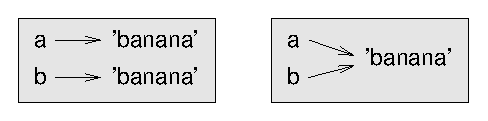
\includegraphics[keepaspectratio,alt={Variables and Objects},height=0.5in]{../images/list1.eps}}
\caption{Variables and Objects}
\end{figure}

Sa isang kaso, ang \texttt{a} at \texttt{b} ay tumutukoy sa dalawang
magkaibang objects na may parehong value. Sa pangalawang kaso, tumutukoy
sila sa parehong object.

\index{is operator} \index{operator!is}

Para suriin kung ang dalawang variables ay tumutukoy sa parehong object,
maaari mong gamitin ang \texttt{is} operator.

\begin{Shaded}
\begin{Highlighting}[]
\OperatorTok{\textgreater{}\textgreater{}\textgreater{}}\NormalTok{ a }\OperatorTok{=} \StringTok{\textquotesingle{}banana\textquotesingle{}}
\OperatorTok{\textgreater{}\textgreater{}\textgreater{}}\NormalTok{ b }\OperatorTok{=} \StringTok{\textquotesingle{}banana\textquotesingle{}}
\OperatorTok{\textgreater{}\textgreater{}\textgreater{}}\NormalTok{ a }\KeywordTok{is}\NormalTok{ b}
\VariableTok{True}
\end{Highlighting}
\end{Shaded}

Sa halimbawang ito, ang Python ay gumawa lang ng isang string object, at
pareho ang \texttt{a} at \texttt{b} ay tumutukoy dito.

Pero kapag gumawa ka ng dalawang lists, makakakuha ka ng dalawang
objects:

\begin{Shaded}
\begin{Highlighting}[]
\OperatorTok{\textgreater{}\textgreater{}\textgreater{}}\NormalTok{ a }\OperatorTok{=}\NormalTok{ [}\DecValTok{1}\NormalTok{, }\DecValTok{2}\NormalTok{, }\DecValTok{3}\NormalTok{]}
\OperatorTok{\textgreater{}\textgreater{}\textgreater{}}\NormalTok{ b }\OperatorTok{=}\NormalTok{ [}\DecValTok{1}\NormalTok{, }\DecValTok{2}\NormalTok{, }\DecValTok{3}\NormalTok{]}
\OperatorTok{\textgreater{}\textgreater{}\textgreater{}}\NormalTok{ a }\KeywordTok{is}\NormalTok{ b}
\VariableTok{False}
\end{Highlighting}
\end{Shaded}

Sa kasong ito sasabihin natin na ang dalawang lists ay
\emph{equivalent}, dahil mayroon silang parehong elements, pero hindi
\emph{identical}, dahil hindi sila parehong object. Kung ang dalawang
objects ay identical, equivalent din sila, pero kung equivalent sila,
hindi naman sila kinakailangang identical.

\index{equivalence} \index{identity}

Hanggang ngayon, ginagamit natin ang ``object'' at ``value'' nang
magkakapalit, pero mas tumpak na sabihin na ang object ay may value.
Kung e-execute mo ang \texttt{a\ =\ {[}1,2,3{]}}, ang \texttt{a} ay
tumutukoy sa list object na ang value ay partikular na sequence ng
elements. Kung ang ibang list ay may parehong elements, sasabihin natin
na mayroon itong parehong value.

\index{object} \index{value}

\section{Aliasing}\label{aliasing}

\index{aliasing} \index{reference!aliasing}

Kung ang \texttt{a} ay tumutukoy sa object at i-assign mo ang
\texttt{b\ =\ a}, pagkatapos parehong variables ay tumutukoy sa parehong
object:

\begin{Shaded}
\begin{Highlighting}[]
\OperatorTok{\textgreater{}\textgreater{}\textgreater{}}\NormalTok{ a }\OperatorTok{=}\NormalTok{ [}\DecValTok{1}\NormalTok{, }\DecValTok{2}\NormalTok{, }\DecValTok{3}\NormalTok{]}
\OperatorTok{\textgreater{}\textgreater{}\textgreater{}}\NormalTok{ b }\OperatorTok{=}\NormalTok{ a}
\OperatorTok{\textgreater{}\textgreater{}\textgreater{}}\NormalTok{ b }\KeywordTok{is}\NormalTok{ a}
\VariableTok{True}
\end{Highlighting}
\end{Shaded}

Ang asosasyon ng variable sa object ay tinatawag na \emph{reference}. Sa
halimbawang ito, mayroong dalawang references sa parehong object.

\index{reference}

Ang object na may higit sa isang reference ay may higit sa isang
pangalan, kaya sinasabi natin na ang object ay \emph{aliased}.

\index{mutability}

Kung ang aliased object ay mutable, ang mga pagbabagong ginawa gamit ang
isang alias ay nakakaapekto sa iba:

\begin{Shaded}
\begin{Highlighting}[]
\OperatorTok{\textgreater{}\textgreater{}\textgreater{}}\NormalTok{ b[}\DecValTok{0}\NormalTok{] }\OperatorTok{=} \DecValTok{17}
\OperatorTok{\textgreater{}\textgreater{}\textgreater{}} \BuiltInTok{print}\NormalTok{(a)}
\NormalTok{[}\DecValTok{17}\NormalTok{, }\DecValTok{2}\NormalTok{, }\DecValTok{3}\NormalTok{]}
\end{Highlighting}
\end{Shaded}

Bagaman ang behavior na ito ay maaaring kapaki-pakinabang, ito ay
madaling magkamali. Sa pangkalahatan, mas ligtas na iwasan ang aliasing
kapag nagtatrabaho ka sa mutable objects.

\index{immutability}

Para sa immutable objects tulad ng strings, ang aliasing ay hindi
gaanong problema. Sa halimbawang ito:

\begin{Shaded}
\begin{Highlighting}[]
\NormalTok{a }\OperatorTok{=} \StringTok{\textquotesingle{}banana\textquotesingle{}}
\NormalTok{b }\OperatorTok{=} \StringTok{\textquotesingle{}banana\textquotesingle{}}
\end{Highlighting}
\end{Shaded}

halos hindi ito gumagawa ng pagkakaiba kung ang \texttt{a} at \texttt{b}
ay tumutukoy sa parehong string o hindi.

\section{List arguments}\label{list-arguments}

\index{list!as argument} \index{argument} \index{argument!list}
\index{reference} \index{parameter}

Kapag nagpasa ka ng list sa function, ang function ay nakakakuha ng
reference sa list. Kung ang function ay nagmo-modify ng list parameter,
nakikita ng caller ang pagbabago. Halimbawa, ang \texttt{delete\_head}
ay nagtatanggal ng unang element mula sa list:

\begin{Shaded}
\begin{Highlighting}[]
\KeywordTok{def}\NormalTok{ delete\_head(t):}
    \KeywordTok{del}\NormalTok{ t[}\DecValTok{0}\NormalTok{]}
\end{Highlighting}
\end{Shaded}

Narito kung paano ito ginagamit:

\begin{Shaded}
\begin{Highlighting}[]
\OperatorTok{\textgreater{}\textgreater{}\textgreater{}}\NormalTok{ letters }\OperatorTok{=}\NormalTok{ [}\StringTok{\textquotesingle{}a\textquotesingle{}}\NormalTok{, }\StringTok{\textquotesingle{}b\textquotesingle{}}\NormalTok{, }\StringTok{\textquotesingle{}c\textquotesingle{}}\NormalTok{]}
\OperatorTok{\textgreater{}\textgreater{}\textgreater{}}\NormalTok{ delete\_head(letters)}
\OperatorTok{\textgreater{}\textgreater{}\textgreater{}} \BuiltInTok{print}\NormalTok{(letters)}
\NormalTok{[}\StringTok{\textquotesingle{}b\textquotesingle{}}\NormalTok{, }\StringTok{\textquotesingle{}c\textquotesingle{}}\NormalTok{]}
\end{Highlighting}
\end{Shaded}

Ang parameter na \texttt{t} at ang variable na \texttt{letters} ay
aliases para sa parehong object.

Mahalagang makilala ang pagkakaiba sa pagitan ng operations na
nagmo-modify ng lists at operations na gumagawa ng bagong lists.
Halimbawa, ang \texttt{append} method ay nagmo-modify ng list, pero ang
\texttt{+} operator ay gumagawa ng bagong list:

\index{append method} \index{method!append} \index{list!concatenation}
\index{concatenation!list}

\begin{Shaded}
\begin{Highlighting}[]
\OperatorTok{\textgreater{}\textgreater{}\textgreater{}}\NormalTok{ t1 }\OperatorTok{=}\NormalTok{ [}\DecValTok{1}\NormalTok{, }\DecValTok{2}\NormalTok{]}
\OperatorTok{\textgreater{}\textgreater{}\textgreater{}}\NormalTok{ t2 }\OperatorTok{=}\NormalTok{ t1.append(}\DecValTok{3}\NormalTok{)}
\OperatorTok{\textgreater{}\textgreater{}\textgreater{}} \BuiltInTok{print}\NormalTok{(t1)}
\NormalTok{[}\DecValTok{1}\NormalTok{, }\DecValTok{2}\NormalTok{, }\DecValTok{3}\NormalTok{]}
\OperatorTok{\textgreater{}\textgreater{}\textgreater{}} \BuiltInTok{print}\NormalTok{(t2)}
\VariableTok{None}

\OperatorTok{\textgreater{}\textgreater{}\textgreater{}}\NormalTok{ t3 }\OperatorTok{=}\NormalTok{ t1 }\OperatorTok{+}\NormalTok{ [}\DecValTok{3}\NormalTok{]}
\OperatorTok{\textgreater{}\textgreater{}\textgreater{}} \BuiltInTok{print}\NormalTok{(t3)}
\NormalTok{[}\DecValTok{1}\NormalTok{, }\DecValTok{2}\NormalTok{, }\DecValTok{3}\NormalTok{]}
\OperatorTok{\textgreater{}\textgreater{}\textgreater{}}\NormalTok{ t1 }\KeywordTok{is}\NormalTok{ t3}
\VariableTok{False}
\end{Highlighting}
\end{Shaded}

Ang pagkakaibang ito ay mahalaga kapag sumusulat ka ng functions na
dapat mag-modify ng lists. Halimbawa, ang function na ito \emph{hindi}
nagtatanggal ng head ng list:

\begin{Shaded}
\begin{Highlighting}[]
\KeywordTok{def}\NormalTok{ bad\_delete\_head(t):}
\NormalTok{    t }\OperatorTok{=}\NormalTok{ t[}\DecValTok{1}\NormalTok{:]              }\CommentTok{\# WRONG!}
\end{Highlighting}
\end{Shaded}

Ang slice operator ay gumagawa ng bagong list at ang assignment ay
ginagawang ang \texttt{t} ay tumutukoy dito, pero wala sa mga iyon ang
may epekto sa list na ipinasa bilang argument.

\index{slice operator} \index{operator!slice}

Ang alternatibo ay sumulat ng function na gumagawa at nagre-return ng
bagong list. Halimbawa, ang \texttt{tail} ay nagre-return ng lahat
maliban sa unang element ng list:

\begin{Shaded}
\begin{Highlighting}[]
\KeywordTok{def}\NormalTok{ tail(t):}
    \ControlFlowTok{return}\NormalTok{ t[}\DecValTok{1}\NormalTok{:]}
\end{Highlighting}
\end{Shaded}

Ang function na ito ay nag-iiwan sa original list na hindi nabago.
Narito kung paano ito ginagamit:

\begin{Shaded}
\begin{Highlighting}[]
\OperatorTok{\textgreater{}\textgreater{}\textgreater{}}\NormalTok{ letters }\OperatorTok{=}\NormalTok{ [}\StringTok{\textquotesingle{}a\textquotesingle{}}\NormalTok{, }\StringTok{\textquotesingle{}b\textquotesingle{}}\NormalTok{, }\StringTok{\textquotesingle{}c\textquotesingle{}}\NormalTok{]}
\OperatorTok{\textgreater{}\textgreater{}\textgreater{}}\NormalTok{ rest }\OperatorTok{=}\NormalTok{ tail(letters)}
\OperatorTok{\textgreater{}\textgreater{}\textgreater{}} \BuiltInTok{print}\NormalTok{(rest)}
\NormalTok{[}\StringTok{\textquotesingle{}b\textquotesingle{}}\NormalTok{, }\StringTok{\textquotesingle{}c\textquotesingle{}}\NormalTok{]}
\end{Highlighting}
\end{Shaded}

\textbf{Exercise 1:} Sumulat ng function na tinatawag na \texttt{chop}
na tumatanggap ng list at nagmo-modify nito, tinatanggal ang una at
huling elements, at nagre-return ng \texttt{None}. Pagkatapos sumulat ng
function na tinatawag na \texttt{middle} na tumatanggap ng list at
nagre-return ng bagong list na naglalaman ng lahat maliban sa una at
huling elements.

\section{Debugging}\label{debugging-7}

\index{debugging}

Ang pabayang paggamit ng lists (at iba pang mutable objects) ay maaaring
magdulot ng mahabang oras ng debugging. Narito ang ilang karaniwang
pitfalls at paraan para iwasan ang mga ito:

\begin{enumerate}
\def\labelenumi{\arabic{enumi}.}
\item
  Huwag kalimutan na karamihan ng list methods ay nagmo-modify ng
  argument at nagre-return ng \texttt{None}. Ito ay kabaligtaran ng
  string methods, na nagre-return ng bagong string at nag-iiwan sa
  original.

  Kung sanay ka sa pagsusulat ng string code tulad nito:

\begin{Shaded}
\begin{Highlighting}[]
\NormalTok{word }\OperatorTok{=}\NormalTok{ word.strip()}
\end{Highlighting}
\end{Shaded}

  Nakakaakit na sumulat ng list code tulad nito:

\begin{Shaded}
\begin{Highlighting}[]
\NormalTok{t }\OperatorTok{=}\NormalTok{ t.sort()           }\CommentTok{\# WRONG!}
\end{Highlighting}
\end{Shaded}

  \index{sort method} \index{method!sort}

  Dahil ang \texttt{sort} ay nagre-return ng \texttt{None}, ang susunod
  na operation na gagawin mo sa \texttt{t} ay malamang na mabibigo.

  Bago gamitin ang list methods at operators, dapat mong basahin nang
  mabuti ang documentation at pagkatapos i-test ang mga ito sa
  interactive mode. Ang methods at operators na ibinabahagi ng lists sa
  iba pang sequences (tulad ng strings) ay na-document sa:

  \href{https://docs.python.org/library/stdtypes.html\#common-sequence-operations}{docs.python.org/library/stdtypes.html\#common-sequence-operations}

  Ang methods at operators na applicable lang sa mutable sequences ay
  na-document sa:

  \href{https://docs.python.org/library/stdtypes.html\#mutable-sequence-types}{docs.python.org/library/stdtypes.html\#mutable-sequence-types}
\item
  Pumili ng idiom at manatili dito.

  \index{idiom}

  Parte ng problema sa lists ay napakaraming paraan para gawin ang mga
  bagay. Halimbawa, para tanggalin ang element mula sa list, maaari mong
  gamitin ang \texttt{pop}, \texttt{remove}, \texttt{del}, o kahit slice
  assignment.

  Para magdagdag ng element, maaari mong gamitin ang \texttt{append}
  method o ang \texttt{+} operator. Pero huwag kalimutan na ang mga ito
  ay tama:

\begin{Shaded}
\begin{Highlighting}[]
\NormalTok{t.append(x)}
\NormalTok{t }\OperatorTok{=}\NormalTok{ t }\OperatorTok{+}\NormalTok{ [x]}
\end{Highlighting}
\end{Shaded}

  At ang mga ito ay mali:

\begin{Shaded}
\begin{Highlighting}[]
\NormalTok{t.append([x])          }\CommentTok{\# WRONG!}
\NormalTok{t }\OperatorTok{=}\NormalTok{ t.append(x)        }\CommentTok{\# WRONG!}
\NormalTok{t }\OperatorTok{+}\NormalTok{ [x]                }\CommentTok{\# WRONG!}
\NormalTok{t }\OperatorTok{=}\NormalTok{ t }\OperatorTok{+}\NormalTok{ x              }\CommentTok{\# WRONG!}
\end{Highlighting}
\end{Shaded}

  Subukan ang bawat isa sa mga halimbawang ito sa interactive mode para
  masiguro na naiintindihan mo ang ginagawa nila. Pansinin na ang huli
  lang ang nagdudulot ng runtime error; ang iba pang tatlo ay legal,
  pero mali ang ginagawa nila.
\item
  Gumawa ng copies para iwasan ang aliasing.

  \index{aliasing!copying to avoid} \index{copy!to avoid aliasing}

  Kung gusto mong gamitin ang method tulad ng \texttt{sort} na
  nagmo-modify ng argument, pero kailangan mo ring panatilihin ang
  original list, maaari kang gumawa ng kopya.

\begin{Shaded}
\begin{Highlighting}[]
\NormalTok{orig }\OperatorTok{=}\NormalTok{ t[:]}
\NormalTok{t.sort()}
\end{Highlighting}
\end{Shaded}

  Sa halimbawang ito maaari mo ring gamitin ang built-in function na
  \texttt{sorted}, na nagre-return ng bagong, sorted list at nag-iiwan
  sa original. Pero sa kasong iyon dapat mong iwasan ang paggamit ng
  \texttt{sorted} bilang variable name!
\item
  Lists, \texttt{split}, at files

  Kapag nagbabasa at nagpa-parse tayo ng files, maraming pagkakataon na
  makatagpo ng input na maaaring i-crash ang program natin kaya
  magandang ideya na muling bisitahin ang \emph{guardian} pattern
  pagdating sa pagsusulat ng programs na nagbabasa sa file at naghahanap
  ng ``needle in the haystack''.

  Muling bisitahin natin ang program natin na naghahanap ng araw ng
  linggo sa from lines ng file natin:

{\small
\begin{verbatim}
From stephen.marquard@uct.ac.za Sat Jan  5 09:14:16 2008
\end{verbatim}
}

  Dahil hinahati natin ang linyang ito sa mga salita, maaari nating
  alisin ang paggamit ng \texttt{startswith} at simpleng tingnan ang
  unang salita ng linya para matukoy kung interesado tayo sa linya.
  Maaari nating gamitin ang \texttt{continue} para laktawan ang mga
  linyang walang ``From'' bilang unang salita tulad ng sumusunod:

\begin{Shaded}
\begin{Highlighting}[]
\NormalTok{fhand }\OperatorTok{=} \BuiltInTok{open}\NormalTok{(}\StringTok{\textquotesingle{}mbox{-}short.txt\textquotesingle{}}\NormalTok{)}
\ControlFlowTok{for}\NormalTok{ line }\KeywordTok{in}\NormalTok{ fhand:}
\NormalTok{    words }\OperatorTok{=}\NormalTok{ line.split()}
    \ControlFlowTok{if}\NormalTok{ words[}\DecValTok{0}\NormalTok{] }\OperatorTok{!=} \StringTok{\textquotesingle{}From\textquotesingle{}}\NormalTok{ : }\ControlFlowTok{continue}
    \BuiltInTok{print}\NormalTok{(words[}\DecValTok{2}\NormalTok{])}
\end{Highlighting}
\end{Shaded}

  Mukhang mas simple ito at hindi na natin kailangan gawin ang
  \texttt{rstrip} para tanggalin ang newline sa dulo ng file. Pero mas
  mabuti ba ito?

{\small
\begin{verbatim}
python search8.py
Sat
Traceback (most recent call last):
  File "search8.py", line 5, in <module>
    if words[0] != 'From' : continue
IndexError: list index out of range
\end{verbatim}
}

  Medyo gumagana ito at nakikita natin ang araw mula sa unang linya
  (Sat), pero pagkatapos nabibigo ang program na may traceback error.
  Ano ang naging mali? Ano ang messed-up data na nagdulot na ang
  elegant, clever, at napaka-Pythonic program natin ay mabigo?

  Maaari mong titigan ito nang mahabang panahon at pag-isipan o
  magtanong sa iba para sa tulong, pero ang mas mabilis at mas
  matalinong approach ay magdagdag ng \texttt{print} statement. Ang
  pinakamabuting lugar para magdagdag ng print statement ay mismo bago
  ang linya kung saan nabigo ang program at mag-print ng data na tila
  nagdudulot ng pagkabigo.

  Ngayon ang approach na ito ay maaaring gumawa ng maraming linya ng
  output, pero hindi bababa ay mayroon ka agad na clue tungkol sa
  problema. Kaya nagdadagdag tayo ng print ng variable na \texttt{words}
  mismo bago ang line five. Nagdadagdag pa tayo ng prefix na ``Debug:''
  sa linya para ma-separate natin ang regular output natin mula sa debug
  output natin.

\begin{Shaded}
\begin{Highlighting}[]
\ControlFlowTok{for}\NormalTok{ line }\KeywordTok{in}\NormalTok{ fhand:}
\NormalTok{    words }\OperatorTok{=}\NormalTok{ line.split()}
    \BuiltInTok{print}\NormalTok{(}\StringTok{\textquotesingle{}Debug:\textquotesingle{}}\NormalTok{, words)}
    \ControlFlowTok{if}\NormalTok{ words[}\DecValTok{0}\NormalTok{] }\OperatorTok{!=} \StringTok{\textquotesingle{}From\textquotesingle{}}\NormalTok{ : }\ControlFlowTok{continue}
    \BuiltInTok{print}\NormalTok{(words[}\DecValTok{2}\NormalTok{])}
\end{Highlighting}
\end{Shaded}

  Kapag tumatakbo ang program, maraming output ang nag-scroll sa screen
  pero sa dulo, nakikita natin ang debug output natin at ang traceback
  kaya alam natin kung ano ang nangyari mismo bago ang traceback.

{\small
\begin{verbatim}
Debug: ['X-DSPAM-Confidence:', '0.8475']
Debug: ['X-DSPAM-Probability:', '0.0000']
Debug: []
Traceback (most recent call last):
  File "search9.py", line 6, in <module>
    if words[0] != 'From' : continue
IndexError: list index out of range
\end{verbatim}
}

  Ang bawat debug line ay nagpi-print ng list ng mga salita na nakukuha
  natin kapag \texttt{split} natin ang linya sa mga salita. Kapag
  nabibigo ang program, ang list ng mga salita ay empty \texttt{{[}{]}}.
  Kung bubuksan natin ang file sa text editor at titingnan ang file, sa
  puntong iyon mukhang ganito:

{\small
\begin{verbatim}
X-DSPAM-Result: Innocent
X-DSPAM-Processed: Sat Jan  5 09:14:16 2008
X-DSPAM-Confidence: 0.8475
X-DSPAM-Probability: 0.0000

Details: http://source.sakaiproject.org/viewsvn/?view=rev&rev=39772
\end{verbatim}
}

  Ang error ay nangyayari kapag ang program natin ay nakatagpo ng blank
  line! Siyempre mayroong ``zero words'' sa blank line. Bakit hindi
  natin naisip iyon kapag sumusulat tayo ng code? Kapag ang code ay
  naghahanap ng unang salita (\texttt{word{[}0{]}}) para suriin kung
  tumutugma ito sa ``From'', nakakakuha tayo ng ``index out of range''
  error.

  Ito siyempre ay perpektong lugar para magdagdag ng ilang
  \emph{guardian} code para iwasan ang pag-check ng unang salita kung
  ang unang salita ay wala doon. Mayroong maraming paraan para
  protektahan ang code na ito; pipiliin nating suriin ang bilang ng mga
  salita na mayroon tayo bago tingnan ang unang salita:

\begin{Shaded}
\begin{Highlighting}[]
\NormalTok{fhand }\OperatorTok{=} \BuiltInTok{open}\NormalTok{(}\StringTok{\textquotesingle{}mbox{-}short.txt\textquotesingle{}}\NormalTok{)}
\NormalTok{count }\OperatorTok{=} \DecValTok{0}
\ControlFlowTok{for}\NormalTok{ line }\KeywordTok{in}\NormalTok{ fhand:}
\NormalTok{    words }\OperatorTok{=}\NormalTok{ line.split()}
    \CommentTok{\# print(\textquotesingle{}Debug:\textquotesingle{}, words)}
    \ControlFlowTok{if} \BuiltInTok{len}\NormalTok{(words) }\OperatorTok{==} \DecValTok{0}\NormalTok{ : }\ControlFlowTok{continue}
    \ControlFlowTok{if}\NormalTok{ words[}\DecValTok{0}\NormalTok{] }\OperatorTok{!=} \StringTok{\textquotesingle{}From\textquotesingle{}}\NormalTok{ : }\ControlFlowTok{continue}
    \BuiltInTok{print}\NormalTok{(words[}\DecValTok{2}\NormalTok{])}
\end{Highlighting}
\end{Shaded}

  Una nag-comment out tayo ng debug print statement sa halip na
  tanggalin ito, kung sakaling mabigo ang modification natin at
  kailangan nating mag-debug ulit. Pagkatapos nagdagdag tayo ng guardian
  statement na sumusuri kung mayroon tayong zero words, at kung gayon,
  ginagamit natin ang \texttt{continue} para laktawan ang susunod na
  linya sa file.

  Maaari nating isipin ang dalawang \texttt{continue} statements bilang
  tumutulong sa atin na pinuhin ang set ng mga linya na ``interesting''
  sa atin at na gusto nating i-process pa. Ang linya na walang salita ay
  ``uninteresting'' sa atin kaya nilalaktawan natin ang susunod na
  linya. Ang linya na walang ``From'' bilang unang salita ay
  uninteresting sa atin kaya nilalaktawan natin ito.

  Ang program na nabago ay tumatakbo nang matagumpay, kaya marahil tama
  ito. Ang guardian statement natin ay sinisiguro na ang
  \texttt{words{[}0{]}} ay hindi kailanman mabibigo, pero marahil hindi
  ito sapat. Kapag nagpo-program tayo, dapat palaging iniisip natin,
  ``Ano ang maaaring maging mali?''
\end{enumerate}

\textbf{Exercise 2:} Alamin kung aling linya ng program sa itaas ang
hindi pa rin properly guarded. Tingnan kung maaari mong gumawa ng text
file na nagdudulot na ang program ay mabigo at pagkatapos baguhin ang
program para ang linya ay properly guarded at i-test ito para masiguro
na ha-handle nito ang bagong text file mo.

\textbf{Exercise 3:} Muling isulat ang guardian code sa halimbawa sa
itaas nang walang dalawang \texttt{if} statements. Sa halip, gumamit ng
compound logical expression gamit ang \texttt{or} logical operator na
may isang \texttt{if} statement.

\section{Glossary}\label{glossary-7}

\begin{description}
\tightlist
\item[aliasing]
Kalagayan kung saan ang dalawa o higit pang variables ay tumutukoy sa
parehong object. \index{aliasing}
\item[delimiter]
Character o string na ginagamit para ipahiwatig kung saan dapat hatiin
ang string. \index{delimiter}
\item[element]
Isa sa mga values sa list (o iba pang sequence); tinatawag din na items.
\index{element}
\item[equivalent]
May parehong value. \index{equivalent}
\item[index]
Integer value na tumutukoy sa element sa list. \index{index} \index{}
\item[identical]
Parehong object (na nagpapahiwatig ng equivalence). \index{identical}
\item[list]
Sequence ng values. \index{list}
\item[list traversal]
Ang sequential na pag-access sa bawat element sa list.
\index{list!traversal}
\item[nested list]
List na element ng ibang list. \index{nested list}
\item[object]
Isang bagay na maaaring tinukoy ng variable. Ang object ay may type at
value. \index{object}
\item[reference]
Ang asosasyon sa pagitan ng variable at value nito. \index{reference}
\end{description}

\section{Exercises}\label{exercises-7}

\index{Romeo and Juliet}

\textbf{Exercise 4: Find all unique words in a file}

Gumamit si Shakespeare ng higit sa 20,000 salita sa kanyang mga gawa.
Pero paano mo matutukoy iyon? Paano mo gagawin ang list ng lahat ng
salitang ginamit ni Shakespeare? I-do-download mo ba lahat ng kanyang
gawa, basahin ito at subaybayan ang lahat ng unique words nang
manu-mano?

Gamitin natin ang Python para makamit iyon sa halip. I-list ang lahat ng
unique words, na naka-sort sa alphabetical order, na naka-store sa file
na \texttt{romeo.txt} na naglalaman ng subset ng gawa ni Shakespeare.

Para makapagsimula, i-download ang kopya ng file
\href{http://www.py4e.com/code3/romeo.txt}{www.py4e.com/code3/romeo.txt}.
Gumawa ng list ng unique words, na maglalaman ng final result. Sumulat
ng program para buksan ang file na \texttt{romeo.txt} at basahin ito
nang linya sa linya. Para sa bawat linya, hatiin ang linya sa list ng
mga salita gamit ang \texttt{split} function. Para sa bawat salita,
suriin kung ang salita ay nasa list na ng unique words. Kung ang salita
ay wala sa list ng unique words, idagdag ito sa list. Kapag natapos ang
program, i-sort at i-print ang list ng unique words sa alphabetical
order.

{\small
\begin{verbatim}
Enter file: romeo.txt
['Arise', 'But', 'It', 'Juliet', 'Who', 'already',
'and', 'breaks', 'east', 'envious', 'fair', 'grief',
'is', 'kill', 'light', 'moon', 'pale', 'sick', 'soft',
'sun', 'the', 'through', 'what', 'window',
'with', 'yonder']
\end{verbatim}
}

\textbf{Exercise 5: Minimalist Email Client.}

Ang MBOX (mail box) ay popular na file format para i-store at ibahagi
ang koleksyon ng emails. Ito ay ginamit ng mga naunang email servers at
desktop apps. Nang hindi pumapasok sa masyadong maraming detalye, ang
MBOX ay text file, na nag-i-store ng emails nang sunud-sunod. Ang mga
emails ay pinaghihiwalay ng espesyal na linya na nagsisimula sa
\texttt{From} (pansinin ang space). Mahalaga, ang mga linyang
nagsisimula sa \texttt{From:} (pansinin ang colon) ay naglalarawan sa
email mismo at hindi kumikilos bilang separator. Isipin na sumulat ka ng
minimalist email app, na nagli-list ng email ng mga sender sa Inbox ng
user at nagbi-bilang ng bilang ng emails.

Sumulat ng program para magbasa sa mail box data at kapag nakakita ka ng
linya na nagsisimula sa ``From'', hahatiin mo ang linya sa mga salita
gamit ang \texttt{split} function. Interesado tayo sa kung sino ang
nagpadala ng mensahe, na siyang pangalawang salita sa From line.

{\small
\begin{verbatim}
From stephen.marquard@uct.ac.za Sat Jan 5 09:14:16 2008
\end{verbatim}
}

I-parse mo ang From line at mag-print ng pangalawang salita para sa
bawat From line, pagkatapos magbi-bilang ka rin ng bilang ng From (hindi
From:) lines at mag-print ng bilang sa dulo. Ito ay magandang sample
output na may ilang linya na tinanggal:

{\small
\begin{verbatim}
python fromcount.py
Enter a file name: mbox-short.txt
stephen.marquard@uct.ac.za
louis@media.berkeley.edu
zqian@umich.edu

[...some output removed...]

ray@media.berkeley.edu
cwen@iupui.edu
cwen@iupui.edu
cwen@iupui.edu
There were 27 lines in the file with From as the first word
\end{verbatim}
}

\textbf{Exercise 6:}

Muling isulat ang program na nagpo-prompt sa user para sa list ng
numbers at nagpi-print ng maximum at minimum ng numbers sa dulo kapag
ang user ay nag-e-enter ng ``done''. Sumulat ng program para i-store ang
numbers na ini-enter ng user sa list at gamitin ang \texttt{max()} at
\texttt{min()} functions para mag-compute ng maximum at minimum numbers
pagkatapos matapos ang loop.

{\small
\begin{verbatim}
Enter a number: 6
Enter a number: 2
Enter a number: 9
Enter a number: 3
Enter a number: 5
Enter a number: done
Maximum: 9.0
Minimum: 2.0
\end{verbatim}
}

\chapter{Dictionaries}\label{dictionaries}

\index{dictionary} \index{dictionary}

\index{type!dict} \index{key} \index{key-value pair} \index{index}
\index{}

Ang \emph{dictionary} ay katulad ng list, pero mas pangkalahatan. Sa
list, ang index positions ay dapat integers; sa dictionary, ang indices
ay maaaring (halos) anumang type.

Maaari mong isipin ang dictionary bilang mapping sa pagitan ng set ng
indices (na tinatawag na \emph{keys}) at set ng values. Ang bawat key ay
nagma-map sa value. Ang asosasyon ng key at value ay tinatawag na
\emph{key-value pair} o minsan \emph{item}.

Bilang halimbawa, gagawa tayo ng dictionary na nagma-map mula sa English
patungo sa Spanish words, kaya ang keys at values ay lahat strings.

Ang function na \texttt{dict} ay gumagawa ng bagong dictionary na walang
items. Dahil ang \texttt{dict} ay pangalan ng built-in function, dapat
mong iwasan ang paggamit nito bilang variable name.

\index{dict function} \index{function!dict}

\begin{Shaded}
\begin{Highlighting}[]
\OperatorTok{\textgreater{}\textgreater{}\textgreater{}}\NormalTok{ eng2sp }\OperatorTok{=} \BuiltInTok{dict}\NormalTok{()}
\OperatorTok{\textgreater{}\textgreater{}\textgreater{}} \BuiltInTok{print}\NormalTok{(eng2sp)}
\NormalTok{\{\}}
\end{Highlighting}
\end{Shaded}

Ang curly brackets, \texttt{\{\}}, ay kumakatawan sa empty dictionary.
Para magdagdag ng items sa dictionary, maaari mong gamitin ang square
brackets:

\index{squiggly bracket} \index{bracket!squiggly}

\begin{Shaded}
\begin{Highlighting}[]
\OperatorTok{\textgreater{}\textgreater{}\textgreater{}}\NormalTok{ eng2sp[}\StringTok{\textquotesingle{}one\textquotesingle{}}\NormalTok{] }\OperatorTok{=} \StringTok{\textquotesingle{}uno\textquotesingle{}}
\end{Highlighting}
\end{Shaded}

Ang linyang ito ay gumagawa ng item na nagma-map mula sa key na
\texttt{\textquotesingle{}one\textquotesingle{}} patungo sa value na
``uno''. Kung magpi-print tayo ng dictionary ulit, nakikita natin ang
key-value pair na may colon sa pagitan ng key at value:

\begin{Shaded}
\begin{Highlighting}[]
\OperatorTok{\textgreater{}\textgreater{}\textgreater{}} \BuiltInTok{print}\NormalTok{(eng2sp)}
\NormalTok{\{}\StringTok{\textquotesingle{}one\textquotesingle{}}\NormalTok{: }\StringTok{\textquotesingle{}uno\textquotesingle{}}\NormalTok{\}}
\end{Highlighting}
\end{Shaded}

Ang output format na ito ay input format din. Halimbawa, maaari kang
gumawa ng bagong dictionary na may tatlong items.

\begin{Shaded}
\begin{Highlighting}[]
\OperatorTok{\textgreater{}\textgreater{}\textgreater{}}\NormalTok{ eng2sp }\OperatorTok{=}\NormalTok{ \{}\StringTok{\textquotesingle{}one\textquotesingle{}}\NormalTok{: }\StringTok{\textquotesingle{}uno\textquotesingle{}}\NormalTok{, }\StringTok{\textquotesingle{}two\textquotesingle{}}\NormalTok{: }\StringTok{\textquotesingle{}dos\textquotesingle{}}\NormalTok{, }\StringTok{\textquotesingle{}three\textquotesingle{}}\NormalTok{: }\StringTok{\textquotesingle{}tres\textquotesingle{}}\NormalTok{\}}
\OperatorTok{\textgreater{}\textgreater{}\textgreater{}} \BuiltInTok{print}\NormalTok{(eng2sp)}
\NormalTok{\{}\StringTok{\textquotesingle{}one\textquotesingle{}}\NormalTok{: }\StringTok{\textquotesingle{}uno\textquotesingle{}}\NormalTok{, }\StringTok{\textquotesingle{}two\textquotesingle{}}\NormalTok{: }\StringTok{\textquotesingle{}dos\textquotesingle{}}\NormalTok{, }\StringTok{\textquotesingle{}three\textquotesingle{}}\NormalTok{: }\StringTok{\textquotesingle{}tres\textquotesingle{}}\NormalTok{\}}
\end{Highlighting}
\end{Shaded}

Simula sa Python 3.7x ang order ng key-value pairs ay pareho sa input
order nila, i.e.~ang dictionaries ay ordered structures na ngayon.

Pero hindi talaga mahalaga iyon dahil ang elements ng dictionary ay
hindi kailanman na-index gamit ang integer indices. Sa halip, ginagamit
mo ang keys para hanapin ang katumbas na values:

\begin{Shaded}
\begin{Highlighting}[]
\OperatorTok{\textgreater{}\textgreater{}\textgreater{}} \BuiltInTok{print}\NormalTok{(eng2sp[}\StringTok{\textquotesingle{}two\textquotesingle{}}\NormalTok{])}
\CommentTok{\textquotesingle{}dos\textquotesingle{}}
\end{Highlighting}
\end{Shaded}

Ang key na \texttt{\textquotesingle{}two\textquotesingle{}} ay palaging
nagma-map sa value na ``dos'' kaya ang order ng items ay hindi mahalaga.

Kung ang key ay wala sa dictionary, makakakuha ka ng exception:

\index{exception!KeyError} \index{KeyError}

\begin{Shaded}
\begin{Highlighting}[]
\OperatorTok{\textgreater{}\textgreater{}\textgreater{}} \BuiltInTok{print}\NormalTok{(eng2sp[}\StringTok{\textquotesingle{}four\textquotesingle{}}\NormalTok{])}
\PreprocessorTok{KeyError}\NormalTok{: }\StringTok{\textquotesingle{}four\textquotesingle{}}
\end{Highlighting}
\end{Shaded}

Ang \texttt{len} function ay gumagana sa dictionaries; nagre-return ito
ng bilang ng key-value pairs:

\index{len function} \index{function!len}

\begin{Shaded}
\begin{Highlighting}[]
\OperatorTok{\textgreater{}\textgreater{}\textgreater{}} \BuiltInTok{len}\NormalTok{(eng2sp)}
\DecValTok{3}
\end{Highlighting}
\end{Shaded}

Ang \texttt{in} operator ay gumagana sa dictionaries; sinasabi nito sa
iyo kung lumalabas ang isang bagay bilang \emph{key} sa dictionary (ang
paglitaw bilang value ay hindi sapat).

\index{membership!dictionary} \index{in operator} \index{operator!in}

\begin{Shaded}
\begin{Highlighting}[]
\OperatorTok{\textgreater{}\textgreater{}\textgreater{}} \StringTok{\textquotesingle{}one\textquotesingle{}} \KeywordTok{in}\NormalTok{ eng2sp}
\VariableTok{True}
\OperatorTok{\textgreater{}\textgreater{}\textgreater{}} \StringTok{\textquotesingle{}uno\textquotesingle{}} \KeywordTok{in}\NormalTok{ eng2sp}
\VariableTok{False}
\end{Highlighting}
\end{Shaded}

Para makita kung lumalabas ang isang bagay bilang value sa dictionary,
maaari mong gamitin ang method na \texttt{values}, na nagre-return ng
values bilang type na maaaring i-convert sa list, at pagkatapos gamitin
ang \texttt{in} operator:

\index{values method} \index{method!values}

\begin{Shaded}
\begin{Highlighting}[]
\OperatorTok{\textgreater{}\textgreater{}\textgreater{}}\NormalTok{ vals }\OperatorTok{=} \BuiltInTok{list}\NormalTok{(eng2sp.values())}
\OperatorTok{\textgreater{}\textgreater{}\textgreater{}} \StringTok{\textquotesingle{}uno\textquotesingle{}} \KeywordTok{in}\NormalTok{ vals}
\VariableTok{True}
\end{Highlighting}
\end{Shaded}

Ang \texttt{in} operator ay gumagamit ng iba't ibang algorithms para sa
lists at dictionaries. Para sa lists, gumagamit ito ng linear search
algorithm. Habang ang list ay nagiging mas mahaba, ang search time ay
nagiging mas mahaba nang direkta sa proporsyon sa haba ng list. Para sa
dictionaries, ang Python ay gumagamit ng algorithm na tinatawag na
\emph{hash table} na may kapansin-pansing property: ang \texttt{in}
operator ay tumatagal ng halos parehong dami ng panahon anuman ang
bilang ng items sa dictionary. Hindi ko ipapaliwanag kung bakit ang hash
functions ay napaka-magical, pero maaari kang magbasa pa tungkol dito sa
\href{https://wikipedia.org/wiki/Hash_table}{wikipedia.org/wiki/Hash\_table}.\footnote{Kung
  gusto mong matuto pa tungkol sa hash tables, mayroong course sa
  https://www.cc4e.com na nag-e-explore kung paano ang programming
  language na C ay nag-i-implement ng Python dictionary.}

\index{hash table} \index{set membership} \index{membership!set}

\textbf{Exercise 1:} I-download ang kopya ng file

\href{http://www.py4e.com/code3/words.txt}{www.py4e.com/code3/words.txt}

Sumulat ng program na nagbabasa ng mga salita sa \emph{words.txt} at
nag-i-store sa kanila bilang keys sa dictionary. Hindi mahalaga kung ano
ang values ay. Pagkatapos maaari mong gamitin ang \texttt{in} operator
bilang mabilis na paraan para suriin kung ang string ay nasa dictionary.

\section{Dictionary as a set of
counters}\label{dictionary-as-a-set-of-counters}

\index{counter}

Ipagpalagay na binigyan ka ng string at gusto mong bilangin kung ilang
beses lumalabas ang bawat letra. Mayroong ilang paraan na maaari mong
gawin:

\begin{enumerate}
\def\labelenumi{\arabic{enumi}.}
\item
  Maaari kang gumawa ng 26 variables, isa para sa bawat letra ng
  alphabet. Pagkatapos maaari mong daanan ang string at, para sa bawat
  character, i-increment ang katumbas na counter, marahil gamit ang
  chained conditional.
\item
  Maaari kang gumawa ng list na may 26 elements. Pagkatapos maaari mong
  i-convert ang bawat character sa number (gamit ang built-in function
  na \texttt{ord}), gamitin ang number bilang index sa list, at
  i-increment ang naaangkop na counter.
\item
  Maaari kang gumawa ng dictionary na may characters bilang keys at
  counters bilang katumbas na values. Sa unang pagkakataon na makikita
  mo ang character, magdadagdag ka ng item sa dictionary. Pagkatapos
  i-increment mo ang value ng existing item.
\end{enumerate}

Ang bawat isa sa mga opsyon na ito ay gumagawa ng parehong computation,
pero ang bawat isa sa kanila ay nag-i-implement ng computation na iyon
sa ibang paraan.

\index{implementation}

Ang \emph{implementation} ay paraan ng paggawa ng computation; ang ilang
implementations ay mas mabuti kaysa sa iba. Halimbawa, ang advantage ng
dictionary implementation ay hindi natin kailangang malaman nang maaga
kung aling mga letra ang lumalabas sa string at kailangan lang nating
gumawa ng lugar para sa mga letrang lumalabas.

Narito kung ano ang hitsura ng code:

\begin{Shaded}
\begin{Highlighting}[]
\NormalTok{word }\OperatorTok{=} \StringTok{\textquotesingle{}brontosaurus\textquotesingle{}}
\NormalTok{d }\OperatorTok{=} \BuiltInTok{dict}\NormalTok{()}
\ControlFlowTok{for}\NormalTok{ c }\KeywordTok{in}\NormalTok{ word:}
    \ControlFlowTok{if}\NormalTok{ c }\KeywordTok{not} \KeywordTok{in}\NormalTok{ d:}
\NormalTok{        d[c] }\OperatorTok{=} \DecValTok{1}
    \ControlFlowTok{else}\NormalTok{:}
\NormalTok{        d[c] }\OperatorTok{=}\NormalTok{ d[c] }\OperatorTok{+} \DecValTok{1}
\BuiltInTok{print}\NormalTok{(d)}
\end{Highlighting}
\end{Shaded}

Epektibong nagco-compute tayo ng \emph{histogram}, na statistical term
para sa set ng counters (o frequencies).

\index{histogram} \index{frequency} \index{traversal}

Ang \texttt{for} loop ay dumadaan sa string. Sa bawat pagkakataon sa
loop, kung ang \texttt{c} ay wala sa dictionary, gumagawa tayo ng bagong
item na may key na \texttt{c} at initial value na 1 (dahil nakita na
natin ang letrang ito nang isang beses). Kung ang \texttt{c} ay nasa
dictionary na, i-increment natin ang \texttt{d{[}c{]}}.

\index{histogram}

Narito ang output ng program:

{\small
\begin{verbatim}
{'b': 1, 'r': 2, 'o': 2, 'n': 1, 't': 1, 's': 2, 'a': 1, 'u': 2}
\end{verbatim}
}

Ang histogram ay nagpapahiwatig na ang mga letrang ``a'' at ``b'' ay
lumalabas nang isang beses; ang ``o'' ay lumalabas nang dalawang beses,
at iba pa.

\index{get method} \index{method!get}

Ang Dictionaries ay may method na tinatawag na \texttt{get} na
tumatanggap ng key at default value. Kung ang key ay lumalabas sa
dictionary, ang \texttt{get} ay nagre-return ng katumbas na value; kung
hindi, nagre-return ito ng default value. Halimbawa:

\begin{Shaded}
\begin{Highlighting}[]
\OperatorTok{\textgreater{}\textgreater{}\textgreater{}}\NormalTok{ counts }\OperatorTok{=}\NormalTok{ \{ }\StringTok{\textquotesingle{}chuck\textquotesingle{}}\NormalTok{ : }\DecValTok{1}\NormalTok{ , }\StringTok{\textquotesingle{}annie\textquotesingle{}}\NormalTok{ : }\DecValTok{42}\NormalTok{, }\StringTok{\textquotesingle{}jan\textquotesingle{}}\NormalTok{: }\DecValTok{100}\NormalTok{\}}
\OperatorTok{\textgreater{}\textgreater{}\textgreater{}} \BuiltInTok{print}\NormalTok{(counts.get(}\StringTok{\textquotesingle{}jan\textquotesingle{}}\NormalTok{, }\DecValTok{0}\NormalTok{))}
\DecValTok{100}
\OperatorTok{\textgreater{}\textgreater{}\textgreater{}} \BuiltInTok{print}\NormalTok{(counts.get(}\StringTok{\textquotesingle{}tim\textquotesingle{}}\NormalTok{, }\DecValTok{0}\NormalTok{))}
\DecValTok{0}
\end{Highlighting}
\end{Shaded}

Maaari nating gamitin ang \texttt{get} para sumulat ng histogram loop
natin nang mas maikli. Dahil ang \texttt{get} method ay awtomatikong
nagha-handle ng kaso kung saan ang key ay wala sa dictionary, maaari
nating bawasan ang apat na linya sa isa at alisin ang \texttt{if}
statement.

\begin{Shaded}
\begin{Highlighting}[]
\NormalTok{word }\OperatorTok{=} \StringTok{\textquotesingle{}brontosaurus\textquotesingle{}}
\NormalTok{d }\OperatorTok{=} \BuiltInTok{dict}\NormalTok{()}
\ControlFlowTok{for}\NormalTok{ c }\KeywordTok{in}\NormalTok{ word:}
\NormalTok{    d[c] }\OperatorTok{=}\NormalTok{ d.get(c,}\DecValTok{0}\NormalTok{) }\OperatorTok{+} \DecValTok{1}
\BuiltInTok{print}\NormalTok{(d)}
\end{Highlighting}
\end{Shaded}

Ang paggamit ng \texttt{get} method para gawing simple ang counting loop
na ito ay nagiging napakakaraniwang ginagamit na ``idiom'' sa Python at
gagamitin natin ito nang maraming beses sa natitirang bahagi ng libro.
Kaya dapat mong maglaan ng sandali at ihambing ang loop na gumagamit ng
\texttt{if} statement at \texttt{in} operator sa loop na gumagamit ng
\texttt{get} method. Parehong eksaktong ginagawa nila ang parehong
bagay, pero ang isa ay mas maikli.

\index{idiom}

\section{Dictionaries and files}\label{dictionaries-and-files}

Isa sa karaniwang gamit ng dictionary ay bilangin ang occurrence ng mga
salita sa file na may nakasulat na teksto. Magsimula tayo sa
napakasimpleng file ng mga salita na kinuha mula sa teksto ng
\emph{Romeo and Juliet}.

Para sa unang set ng halimbawa, gagamitin natin ang pinaikli at
pinasimpleng bersyon ng teksto na walang punctuation. Mamaya
magtatrabaho tayo sa teksto ng scene na may kasamang punctuation.

{\small
\begin{verbatim}
But soft what light through yonder window breaks
It is the east and Juliet is the sun
Arise fair sun and kill the envious moon
Who is already sick and pale with grief
\end{verbatim}
}

Susulat tayo ng Python program para magbasa sa mga linya ng file, hatiin
ang bawat linya sa list ng mga salita, at pagkatapos mag-loop sa bawat
isa sa mga salita sa linya at bilangin ang bawat salita gamit ang
dictionary.

\index{nested loops} \index{loop!nested}

Makikita mo na mayroon tayong dalawang \texttt{for} loops. Ang outer
loop ay nagbabasa ng mga linya ng file at ang inner loop ay
nag-i-iterate sa bawat isa sa mga salita sa partikular na linya. Ito ay
halimbawa ng pattern na tinatawag na \emph{nested loops} dahil ang isa
sa mga loops ay ang \emph{outer} loop at ang ibang loop ay ang
\emph{inner} loop.

Dahil ang inner loop ay nag-e-execute ng lahat ng iterations nito sa
bawat pagkakataon na ang outer loop ay gumagawa ng isang iteration,
iniisip natin ang inner loop bilang nag-i-iterate nang ``mas mabilis''
at ang outer loop bilang nag-i-iterate nang mas mabagal.

\index{Romeo and Juliet}

Ang kombinasyon ng dalawang nested loops ay sinisiguro na mabibilang
natin ang bawat salita sa bawat linya ng input file.

\begin{Shaded}
\begin{Highlighting}[]
\NormalTok{fname }\OperatorTok{=} \BuiltInTok{input}\NormalTok{(}\StringTok{\textquotesingle{}Enter the file name: \textquotesingle{}}\NormalTok{)}
\ControlFlowTok{try}\NormalTok{:}
\NormalTok{    fhand }\OperatorTok{=} \BuiltInTok{open}\NormalTok{(fname)}
\ControlFlowTok{except}\NormalTok{:}
    \BuiltInTok{print}\NormalTok{(}\StringTok{\textquotesingle{}File cannot be opened:\textquotesingle{}}\NormalTok{, fname)}
\NormalTok{    exit()}

\NormalTok{counts }\OperatorTok{=} \BuiltInTok{dict}\NormalTok{()}
\ControlFlowTok{for}\NormalTok{ line }\KeywordTok{in}\NormalTok{ fhand:}
\NormalTok{    words }\OperatorTok{=}\NormalTok{ line.split()}
    \ControlFlowTok{for}\NormalTok{ word }\KeywordTok{in}\NormalTok{ words:}
        \ControlFlowTok{if}\NormalTok{ word }\KeywordTok{not} \KeywordTok{in}\NormalTok{ counts:}
\NormalTok{            counts[word] }\OperatorTok{=} \DecValTok{1}
        \ControlFlowTok{else}\NormalTok{:}
\NormalTok{            counts[word] }\OperatorTok{+=} \DecValTok{1}

\BuiltInTok{print}\NormalTok{(counts)}

\CommentTok{\# Code: https://www.py4e.com/code3/count1.py}
\end{Highlighting}
\end{Shaded}

\begin{trinketfiles}
../code3/romeo.txt
\end{trinketfiles}

Sa \texttt{else} statement natin, ginagamit natin ang mas compact na
alternatibo para mag-increment ng variable. Ang
\texttt{counts{[}word{]}\ +=\ 1} ay katumbas ng
\texttt{counts{[}word{]}\ =\ counts{[}word{]}\ +\ 1}. Ang alinmang
method ay maaaring gamitin para baguhin ang value ng variable sa anumang
nais na dami. Katulad na alternatibo ang umiiral para sa \texttt{-=},
\texttt{*=}, at \texttt{/=}.

Kapag tumatakbo ang program, nakikita natin ang raw dump ng lahat ng
counts sa unsorted hash order. (ang file na \emph{romeo.txt} ay
available sa
\href{http://www.py4e.com/code3/romeo.txt}{www.py4e.com/code3/romeo.txt})

{\small
\begin{verbatim}
python count1.py
Enter the file name: romeo.txt
{'But': 1, 'soft': 1, 'what': 1, 'light': 1, 'through': 1, 'yonder': 1,
'window': 1, 'breaks': 1, 'It': 1, 'is': 3, 'the': 3, 'east': 1, 'and': 3,
'Juliet': 1, 'sun': 2, 'Arise': 1, 'fair': 1, 'kill': 1, 'envious': 1,
'moon': 1, 'Who': 1, 'already': 1, 'sick': 1, 'pale': 1, 'with': 1,
'grief': 1}
\end{verbatim}
}

Medyo hindi maginhawa na tumingin sa dictionary para hanapin ang pinaka
karaniwang mga salita at ang kanilang counts, kaya kailangan nating
magdagdag ng higit pang Python code para makakuha ng output na mas
makakatulong.

\section{Looping and dictionaries}\label{looping-and-dictionaries}

\index{dictionary!looping with} \index{looping!with dictionaries}
\index{traversal}

Kung gagamitin mo ang dictionary bilang sequence sa \texttt{for}
statement, dumadaan ito sa keys ng dictionary. Ang loop na ito ay
nagpi-print ng bawat key at katumbas na value:

\begin{Shaded}
\begin{Highlighting}[]
\NormalTok{counts }\OperatorTok{=}\NormalTok{ \{ }\StringTok{\textquotesingle{}chuck\textquotesingle{}}\NormalTok{ : }\DecValTok{1}\NormalTok{ , }\StringTok{\textquotesingle{}annie\textquotesingle{}}\NormalTok{ : }\DecValTok{42}\NormalTok{, }\StringTok{\textquotesingle{}jan\textquotesingle{}}\NormalTok{: }\DecValTok{100}\NormalTok{\}}
\ControlFlowTok{for}\NormalTok{ key }\KeywordTok{in}\NormalTok{ counts:}
    \BuiltInTok{print}\NormalTok{(key, counts[key])}
\end{Highlighting}
\end{Shaded}

Narito ang hitsura ng output:

{\small
\begin{verbatim}
chuck 1
annie 42
jan 100
\end{verbatim}
}

Muli, ang keys ay ordered.

\index{idiom}

Maaari nating gamitin ang pattern na ito para i-implement ang iba't
ibang loop idioms na na-describe natin kanina. Halimbawa kung gusto
nating hanapin ang lahat ng entries sa dictionary na may value na higit
sa sampu, maaari tayong sumulat ng sumusunod na code:

\begin{Shaded}
\begin{Highlighting}[]
\NormalTok{counts }\OperatorTok{=}\NormalTok{ \{ }\StringTok{\textquotesingle{}chuck\textquotesingle{}}\NormalTok{ : }\DecValTok{1}\NormalTok{ , }\StringTok{\textquotesingle{}annie\textquotesingle{}}\NormalTok{ : }\DecValTok{42}\NormalTok{, }\StringTok{\textquotesingle{}jan\textquotesingle{}}\NormalTok{: }\DecValTok{100}\NormalTok{\}}
\ControlFlowTok{for}\NormalTok{ key }\KeywordTok{in}\NormalTok{ counts:}
    \ControlFlowTok{if}\NormalTok{ counts[key] }\OperatorTok{\textgreater{}} \DecValTok{10}\NormalTok{ :}
        \BuiltInTok{print}\NormalTok{(key, counts[key])}
\end{Highlighting}
\end{Shaded}

Ang \texttt{for} loop ay nag-i-iterate sa \emph{keys} ng dictionary,
kaya dapat nating gamitin ang index operator para kunin ang katumbas na
\emph{value} para sa bawat key. Narito ang hitsura ng output:

{\small
\begin{verbatim}
annie 42
jan 100
\end{verbatim}
}

Nakikita lang natin ang entries na may value na higit sa 10.

\index{keys method} \index{method!keys}

Kung gusto mong mag-print ng keys sa alphabetical order, una gumawa ka
ng list ng keys sa dictionary gamit ang \texttt{keys} method na
available sa dictionary objects, at pagkatapos i-sort ang list na iyon
at mag-loop sa sorted list, naghahanap ng bawat key at nagpi-print ng
key-value pairs sa sorted order tulad ng sumusunod:

\begin{Shaded}
\begin{Highlighting}[]
\NormalTok{counts }\OperatorTok{=}\NormalTok{ \{ }\StringTok{\textquotesingle{}chuck\textquotesingle{}}\NormalTok{ : }\DecValTok{1}\NormalTok{ , }\StringTok{\textquotesingle{}annie\textquotesingle{}}\NormalTok{ : }\DecValTok{42}\NormalTok{, }\StringTok{\textquotesingle{}jan\textquotesingle{}}\NormalTok{: }\DecValTok{100}\NormalTok{\}}
\NormalTok{lst }\OperatorTok{=} \BuiltInTok{list}\NormalTok{(counts.keys())}
\BuiltInTok{print}\NormalTok{(lst)}
\NormalTok{lst.sort()}
\BuiltInTok{print}\NormalTok{(lst)}
\ControlFlowTok{for}\NormalTok{ key }\KeywordTok{in}\NormalTok{ lst:}
    \BuiltInTok{print}\NormalTok{(key, counts[key])}
\end{Highlighting}
\end{Shaded}

Here's what the output looks like:

{\small
\begin{verbatim}
['chuck', 'annie', 'jan']
['annie', 'chuck', 'jan']
annie 42
chuck 1
jan 100
\end{verbatim}
}

First you see the list of keys in non-alphabetical order that we get
from the \texttt{keys} method. Then we see the key-value pairs in
alphabetical order from the \texttt{for} loop.

\section{Advanced text parsing}\label{advanced-text-parsing}

\index{Romeo and Juliet}

In the above example using the file \emph{romeo.txt}, we made the file
as simple as possible by removing all punctuation by hand. The actual
text has lots of punctuation, as shown below.

{\small
\begin{verbatim}
But, soft! what light through yonder window breaks?
It is the east, and Juliet is the sun.
Arise, fair sun, and kill the envious moon,
Who is already sick and pale with grief,
\end{verbatim}
}

Since the Python \texttt{split} function looks for spaces and treats
words as tokens separated by spaces, we would treat the words ``soft!''
and ``soft'' as \emph{different} words and create a separate dictionary
entry for each word.

Also since the file has capitalization, we would treat ``who'' and
``Who'' as different words with different counts.

We can solve both these problems by using the string methods
\texttt{lower}, \texttt{punctuation}, and \texttt{translate}. The
\texttt{translate} is the most subtle of the methods. Here is the
documentation for \texttt{translate}:

\texttt{line.translate(str.maketrans(fromstr,\ tostr,\ deletestr))}

\emph{Replace the characters in \texttt{fromstr} with the character in
the same position in \texttt{tostr} and delete all characters that are
in \texttt{deletestr}. The \texttt{fromstr} and \texttt{tostr} can be
empty strings and the \texttt{deletestr} parameter can be omitted.}

We will not specify the \texttt{tostr} but we will use the
\texttt{deletestr} parameter to delete all of the punctuation. We will
even let Python tell us the list of characters that it considers
``punctuation'':

\begin{Shaded}
\begin{Highlighting}[]
\OperatorTok{\textgreater{}\textgreater{}\textgreater{}} \ImportTok{import}\NormalTok{ string}
\OperatorTok{\textgreater{}\textgreater{}\textgreater{}}\NormalTok{ string.punctuation}
\CommentTok{\textquotesingle{}!"\#$\%\&}\CharTok{\textbackslash{}\textquotesingle{}}\CommentTok{()*+,{-}./:;\textless{}=\textgreater{}?@[}\CharTok{\textbackslash{}\textbackslash{}}\CommentTok{]\^{}\_\textasciigrave{}\{|\}\textasciitilde{}\textquotesingle{}}
\end{Highlighting}
\end{Shaded}

The parameters used by \texttt{translate} were different in Python 2.0.

We make the following modifications to our program:

\begin{Shaded}
\begin{Highlighting}[]
\ImportTok{import}\NormalTok{ string}

\NormalTok{fname }\OperatorTok{=} \BuiltInTok{input}\NormalTok{(}\StringTok{\textquotesingle{}Enter the file name: \textquotesingle{}}\NormalTok{)}
\ControlFlowTok{try}\NormalTok{:}
\NormalTok{    fhand }\OperatorTok{=} \BuiltInTok{open}\NormalTok{(fname)}
\ControlFlowTok{except}\NormalTok{:}
    \BuiltInTok{print}\NormalTok{(}\StringTok{\textquotesingle{}File cannot be opened:\textquotesingle{}}\NormalTok{, fname)}
\NormalTok{    exit()}

\NormalTok{counts }\OperatorTok{=} \BuiltInTok{dict}\NormalTok{()}
\ControlFlowTok{for}\NormalTok{ line }\KeywordTok{in}\NormalTok{ fhand:}
\NormalTok{    line }\OperatorTok{=}\NormalTok{ line.rstrip()}
    \CommentTok{\# First two parameters are empty strings}
\NormalTok{    line }\OperatorTok{=}\NormalTok{ line.translate(line.maketrans(}\StringTok{""}\NormalTok{, }\StringTok{""}\NormalTok{, string.punctuation))}
\NormalTok{    line }\OperatorTok{=}\NormalTok{ line.lower()}
\NormalTok{    words }\OperatorTok{=}\NormalTok{ line.split()}
    \ControlFlowTok{for}\NormalTok{ word }\KeywordTok{in}\NormalTok{ words:}
        \ControlFlowTok{if}\NormalTok{ word }\KeywordTok{not} \KeywordTok{in}\NormalTok{ counts:}
\NormalTok{            counts[word] }\OperatorTok{=} \DecValTok{1}
        \ControlFlowTok{else}\NormalTok{:}
\NormalTok{            counts[word] }\OperatorTok{+=} \DecValTok{1}

\BuiltInTok{print}\NormalTok{(counts)}

\CommentTok{\# Code: https://www.py4e.com/code3/count2.py}
\end{Highlighting}
\end{Shaded}

\begin{trinketfiles}
../code3/romeo-full.txt
\end{trinketfiles}

Part of learning the ``Art of Python'' or ``Thinking Pythonically'' is
realizing that Python often has built-in capabilities for many common
data analysis problems. Over time, you will see enough example code and
read enough of the documentation to know where to look to see if someone
has already written something that makes your job much easier.

The following is an abbreviated version of the output:

{\small
\begin{verbatim}
Enter the file name: romeo-full.txt
{'romeo': 40, 'and': 42, 'juliet': 32, 'act': 1, '2': 2, 'scene': 2,
'ii': 1, 'capulets': 1, 'orchard': 2, 'enter': 1, 'he': 5, 'jests': 1,
'at': 9, 'scars': 1, 'that': 30, 'never': 2, 'felt': 1, 'a': 24,
'wound': 1, 'appears': 1, 'above': 6, 'window': 2, 'but': 18,
'soft': 1, 'what': 11, 'light': 5, 'through': 2, 'yonder': 2,
'breaks': 1, ...}
\end{verbatim}
}

Looking through this output is still unwieldy and we can use Python to
give us exactly what we are looking for, but to do so, we need to learn
about Python \emph{tuples}. We will pick up this example once we learn
about tuples.

\section{Debugging}\label{debugging-8}

\index{debugging}

As you work with bigger datasets it can become unwieldy to debug by
printing and checking data by hand. Here are some suggestions for
debugging large datasets:

\begin{description}
\item[Scale down the input]
If possible, reduce the size of the dataset. For example if the program
reads a text file, start with just the first 10 lines, or with the
smallest example you can find. You can either edit the files themselves,
or (better) modify the program so it reads only the first \texttt{n}
lines.

If there is an error, you can reduce \texttt{n} to the smallest value
that manifests the error, and then increase it gradually as you find and
correct errors.
\item[Check summaries and types]
Instead of printing and checking the entire dataset, consider printing
summaries of the data: for example, the number of items in a dictionary
or the total of a list of numbers.

A common cause of runtime errors is a value that is not the right type.
For debugging this kind of error, it is often enough to print the type
of a value.
\item[Write self-checks]
Sometimes you can write code to check for errors automatically. For
example, if you are computing the average of a list of numbers, you
could check that the result is not greater than the largest element in
the list or less than the smallest. This is called a ``sanity check''
because it detects results that are ``completely illogical''.
\index{sanity check} \index{consistency check}

Another kind of check compares the results of two different computations
to see if they are consistent. This is called a ``consistency check''.
\item[Pretty print the output]
Formatting debugging output can make it easier to spot an error.
\end{description}

Again, time you spend building scaffolding can reduce the time you spend
debugging. \index{scaffolding}

\section{Glossary}\label{glossary-8}

\begin{description}
\tightlist
\item[dictionary]
A mapping from a set of keys to their corresponding values.
\index{dictionary}
\item[hashtable]
The algorithm used to implement Python dictionaries. \index{hashtable}
\item[hash function]
A function used by a hashtable to compute the location for a key.
\index{hash function}
\item[histogram]
A set of counters. \index{histogram}
\item[implementation]
A way of performing a computation. \index{implementation}
\item[item]
Another name for a key-value pair. \index{item!dictionary}
\item[key]
An object that appears in a dictionary as the first part of a key-value
pair. \index{key}
\item[key-value pair]
The representation of the mapping from a key to a value.
\index{key-value pair}
\item[lookup]
A dictionary operation that takes a key and finds the corresponding
value. \index{lookup}
\item[nested loops]
When there are one or more loops ``inside'' of another loop. The inner
loop runs to completion each time the outer loop runs once.
\index{nested loops} \index{loop!nested}
\item[value]
An object that appears in a dictionary as the second part of a key-value
pair. This is more specific than our previous use of the word ``value''.
\index{value}
\end{description}

\section{Exercises}\label{exercises-8}

\textbf{Exercise 2:} Write a program that categorizes each mail message
by which day of the week the commit was done. To do this look for lines
that start with ``From'', then look for the third word and keep a
running count of each of the days of the week. At the end of the program
print out the contents of your dictionary (order does not matter).

Sample Line:

{\small
\begin{verbatim}
From stephen.marquard@uct.ac.za Sat Jan  5 09:14:16 2008
\end{verbatim}
}

Sample Execution:

{\small
\begin{verbatim}
python dow.py
Enter a file name: mbox-short.txt
{'Fri': 20, 'Thu': 6, 'Sat': 1}
\end{verbatim}
}

\textbf{Exercise 3:} Write a program to read through a mail log, build a
histogram using a dictionary to count how many messages have come from
each email address, and print the dictionary.

{\small
\begin{verbatim}
Enter file name: mbox-short.txt
{'gopal.ramasammycook@gmail.com': 1, 'louis@media.berkeley.edu': 3,
'cwen@iupui.edu': 5, 'antranig@caret.cam.ac.uk': 1,
'rjlowe@iupui.edu': 2, 'gsilver@umich.edu': 3,
'david.horwitz@uct.ac.za': 4, 'wagnermr@iupui.edu': 1,
'zqian@umich.edu': 4, 'stephen.marquard@uct.ac.za': 2,
'ray@media.berkeley.edu': 1}
\end{verbatim}
}

\textbf{Exercise 4:} Add code to the above program to figure out who has
sent the most messages in the file. After all the data has been read and
the dictionary has been created, look through the dictionary using a
maximum loop (see Chapter 5: Maximum and minimum loops) to find who has
the most messages and print how many messages the person has.

{\small
\begin{verbatim}
Enter a file name: mbox-short.txt
cwen@iupui.edu 5

Enter a file name: mbox.txt
zqian@umich.edu 195
\end{verbatim}
}

\textbf{Exercise 5:} This program records the domain name (instead of
the address) where the message was sent from instead of who the mail
came from (i.e., the whole email address). At the end of the program,
print out the contents of your dictionary.

{\small
\begin{verbatim}
python schoolcount.py
Enter a file name: mbox-short.txt
{'media.berkeley.edu': 4, 'uct.ac.za': 6, 'umich.edu': 7,
'gmail.com': 1, 'caret.cam.ac.uk': 1, 'iupui.edu': 8}
\end{verbatim}
}

\chapter{Tuples}\label{tuples}

\section{Tuples are immutable}\label{tuples-are-immutable}

\index{tuple} \index{type!tuple} \index{sequence}

Ang tuple\footnote{Fun fact: Ang salitang ``tuple'' ay nagmula sa mga
  pangalan na ibinigay sa sequences ng mga numero na may iba't ibang
  haba: single, double, triple, quadruple, quintuple, sextuple,
  septuple, etc.} ay sequence ng values na katulad ng list. Ang mga
values na naka-store sa tuple ay maaaring anumang type, at sila ay
na-index ng integers. Ang importanteng pagkakaiba ay ang tuples ay
\emph{immutable}. Ang tuples ay \emph{comparable} din at \emph{hashable}
kaya maaari nating i-sort ang lists ng mga ito at gamitin ang tuples
bilang key values sa Python dictionaries.

\index{mutability} \index{hashable} \index{comparable}
\index{immutability}

Syntactically, ang tuple ay comma-separated list ng values:

\begin{Shaded}
\begin{Highlighting}[]
\OperatorTok{\textgreater{}\textgreater{}\textgreater{}}\NormalTok{ t }\OperatorTok{=} \StringTok{\textquotesingle{}a\textquotesingle{}}\NormalTok{, }\StringTok{\textquotesingle{}b\textquotesingle{}}\NormalTok{, }\StringTok{\textquotesingle{}c\textquotesingle{}}\NormalTok{, }\StringTok{\textquotesingle{}d\textquotesingle{}}\NormalTok{, }\StringTok{\textquotesingle{}e\textquotesingle{}}
\end{Highlighting}
\end{Shaded}

Bagaman hindi ito kailangan, karaniwang i-enclose ang tuples sa
parentheses para matulungan tayong mabilis na makilala ang tuples kapag
tinitingnan natin ang Python code:

\index{parentheses!tuples in}

\begin{Shaded}
\begin{Highlighting}[]
\OperatorTok{\textgreater{}\textgreater{}\textgreater{}}\NormalTok{ t }\OperatorTok{=}\NormalTok{ (}\StringTok{\textquotesingle{}a\textquotesingle{}}\NormalTok{, }\StringTok{\textquotesingle{}b\textquotesingle{}}\NormalTok{, }\StringTok{\textquotesingle{}c\textquotesingle{}}\NormalTok{, }\StringTok{\textquotesingle{}d\textquotesingle{}}\NormalTok{, }\StringTok{\textquotesingle{}e\textquotesingle{}}\NormalTok{)}
\end{Highlighting}
\end{Shaded}

Para gumawa ng tuple na may isang element, kailangan mong isama ang
final comma:

\index{singleton} \index{tuple!singleton}

\begin{Shaded}
\begin{Highlighting}[]
\OperatorTok{\textgreater{}\textgreater{}\textgreater{}}\NormalTok{ t1 }\OperatorTok{=}\NormalTok{ (}\StringTok{\textquotesingle{}a\textquotesingle{}}\NormalTok{,)}
\OperatorTok{\textgreater{}\textgreater{}\textgreater{}} \BuiltInTok{type}\NormalTok{(t1)}
\OperatorTok{\textless{}}\BuiltInTok{type} \StringTok{\textquotesingle{}tuple\textquotesingle{}}\OperatorTok{\textgreater{}}
\end{Highlighting}
\end{Shaded}

Kung walang comma ang Python ay tinatrato ang
\texttt{(\textquotesingle{}a\textquotesingle{})} bilang expression na
may string sa parentheses na nag-e-evaluate sa string:

\begin{Shaded}
\begin{Highlighting}[]
\OperatorTok{\textgreater{}\textgreater{}\textgreater{}}\NormalTok{ t2 }\OperatorTok{=}\NormalTok{ (}\StringTok{\textquotesingle{}a\textquotesingle{}}\NormalTok{)}
\OperatorTok{\textgreater{}\textgreater{}\textgreater{}} \BuiltInTok{type}\NormalTok{(t2)}
\OperatorTok{\textless{}}\BuiltInTok{type} \StringTok{\textquotesingle{}str\textquotesingle{}}\OperatorTok{\textgreater{}}
\end{Highlighting}
\end{Shaded}

Ang isa pang paraan para gumawa ng tuple ay ang built-in function na
\texttt{tuple}. Kung walang argument, gumagawa ito ng empty tuple:

\index{tuple function} \index{function!tuple}

\begin{Shaded}
\begin{Highlighting}[]
\OperatorTok{\textgreater{}\textgreater{}\textgreater{}}\NormalTok{ t }\OperatorTok{=} \BuiltInTok{tuple}\NormalTok{()}
\OperatorTok{\textgreater{}\textgreater{}\textgreater{}} \BuiltInTok{print}\NormalTok{(t)}
\NormalTok{()}
\end{Highlighting}
\end{Shaded}

Kung ang argument ay sequence (string, list, o tuple), ang result ng
pagtawag sa \texttt{tuple} ay tuple na may elements ng sequence:

\begin{Shaded}
\begin{Highlighting}[]
\OperatorTok{\textgreater{}\textgreater{}\textgreater{}}\NormalTok{ t }\OperatorTok{=} \BuiltInTok{tuple}\NormalTok{(}\StringTok{\textquotesingle{}lupins\textquotesingle{}}\NormalTok{)}
\OperatorTok{\textgreater{}\textgreater{}\textgreater{}} \BuiltInTok{print}\NormalTok{(t)}
\NormalTok{(}\StringTok{\textquotesingle{}l\textquotesingle{}}\NormalTok{, }\StringTok{\textquotesingle{}u\textquotesingle{}}\NormalTok{, }\StringTok{\textquotesingle{}p\textquotesingle{}}\NormalTok{, }\StringTok{\textquotesingle{}i\textquotesingle{}}\NormalTok{, }\StringTok{\textquotesingle{}n\textquotesingle{}}\NormalTok{, }\StringTok{\textquotesingle{}s\textquotesingle{}}\NormalTok{)}
\end{Highlighting}
\end{Shaded}

Dahil ang \texttt{tuple} ay pangalan ng constructor, dapat mong iwasan
ang paggamit nito bilang variable name.

Karamihan ng list operators ay gumagana din sa tuples. Ang bracket
operator ay nag-i-index ng element:

\index{bracket operator} \index{operator!bracket}

\begin{Shaded}
\begin{Highlighting}[]
\OperatorTok{\textgreater{}\textgreater{}\textgreater{}}\NormalTok{ t }\OperatorTok{=}\NormalTok{ (}\StringTok{\textquotesingle{}a\textquotesingle{}}\NormalTok{, }\StringTok{\textquotesingle{}b\textquotesingle{}}\NormalTok{, }\StringTok{\textquotesingle{}c\textquotesingle{}}\NormalTok{, }\StringTok{\textquotesingle{}d\textquotesingle{}}\NormalTok{, }\StringTok{\textquotesingle{}e\textquotesingle{}}\NormalTok{)}
\OperatorTok{\textgreater{}\textgreater{}\textgreater{}} \BuiltInTok{print}\NormalTok{(t[}\DecValTok{0}\NormalTok{])}
\CommentTok{\textquotesingle{}a\textquotesingle{}}
\end{Highlighting}
\end{Shaded}

At ang slice operator ay pumipili ng range ng elements.

\index{slice operator} \index{operator!slice} \index{tuple!slice}
\index{slice!tuple}

\begin{Shaded}
\begin{Highlighting}[]
\OperatorTok{\textgreater{}\textgreater{}\textgreater{}} \BuiltInTok{print}\NormalTok{(t[}\DecValTok{1}\NormalTok{:}\DecValTok{3}\NormalTok{])}
\NormalTok{(}\StringTok{\textquotesingle{}b\textquotesingle{}}\NormalTok{, }\StringTok{\textquotesingle{}c\textquotesingle{}}\NormalTok{)}
\end{Highlighting}
\end{Shaded}

Pero kung susubukan mong baguhin ang isa sa elements ng tuple,
makakakuha ka ng error:

\index{exception!TypeError} \index{TypeError} \index{item assignment}
\index{assignment!item}

\begin{Shaded}
\begin{Highlighting}[]
\OperatorTok{\textgreater{}\textgreater{}\textgreater{}}\NormalTok{ t[}\DecValTok{0}\NormalTok{] }\OperatorTok{=} \StringTok{\textquotesingle{}A\textquotesingle{}}
\PreprocessorTok{TypeError}\NormalTok{: }\BuiltInTok{object}\NormalTok{ doesn}\StringTok{\textquotesingle{}t support item assignment}
\end{Highlighting}
\end{Shaded}

Hindi mo maaaring baguhin ang elements ng tuple, pero maaari mong
palitan ang isang tuple ng iba pa:

\begin{Shaded}
\begin{Highlighting}[]
\OperatorTok{\textgreater{}\textgreater{}\textgreater{}}\NormalTok{ t }\OperatorTok{=}\NormalTok{ (}\StringTok{\textquotesingle{}A\textquotesingle{}}\NormalTok{,) }\OperatorTok{+}\NormalTok{ t[}\DecValTok{1}\NormalTok{:]}
\OperatorTok{\textgreater{}\textgreater{}\textgreater{}} \BuiltInTok{print}\NormalTok{(t)}
\NormalTok{(}\StringTok{\textquotesingle{}A\textquotesingle{}}\NormalTok{, }\StringTok{\textquotesingle{}b\textquotesingle{}}\NormalTok{, }\StringTok{\textquotesingle{}c\textquotesingle{}}\NormalTok{, }\StringTok{\textquotesingle{}d\textquotesingle{}}\NormalTok{, }\StringTok{\textquotesingle{}e\textquotesingle{}}\NormalTok{)}
\end{Highlighting}
\end{Shaded}

\section{Comparing tuples}\label{comparing-tuples}

\index{comparison!tuple} \index{tuple!comparison} \index{sort method}
\index{method!sort}

Ang comparison operators ay gumagana sa tuples at iba pang sequences.
Ang Python ay nagsisimula sa pag-compare ng unang element mula sa bawat
sequence. Kung sila ay equal, nagpapatuloy ito sa susunod na element, at
iba pa, hanggang makita ang elements na magkaiba. Ang mga susunod na
elements ay hindi isinasaalang-alang (kahit na talagang malaki sila).

\begin{Shaded}
\begin{Highlighting}[]
\OperatorTok{\textgreater{}\textgreater{}\textgreater{}}\NormalTok{ (}\DecValTok{0}\NormalTok{, }\DecValTok{1}\NormalTok{, }\DecValTok{2}\NormalTok{) }\OperatorTok{\textless{}}\NormalTok{ (}\DecValTok{0}\NormalTok{, }\DecValTok{3}\NormalTok{, }\DecValTok{4}\NormalTok{)}
\VariableTok{True}
\OperatorTok{\textgreater{}\textgreater{}\textgreater{}}\NormalTok{ (}\DecValTok{0}\NormalTok{, }\DecValTok{1}\NormalTok{, }\DecValTok{2000000}\NormalTok{) }\OperatorTok{\textless{}}\NormalTok{ (}\DecValTok{0}\NormalTok{, }\DecValTok{3}\NormalTok{, }\DecValTok{4}\NormalTok{)}
\VariableTok{True}
\end{Highlighting}
\end{Shaded}

Ang \texttt{sort} function ay gumagana sa parehong paraan. Nagso-sort
ito primarily sa pamamagitan ng unang element, pero sa kaso ng tie,
nagso-sort ito sa pamamagitan ng pangalawang element, at iba pa.

Ang feature na ito ay nagpapahintulot sa pattern na tinatawag na
\emph{DSU} para sa

\begin{description}
\tightlist
\item[Decorate]
sequence sa pamamagitan ng paggawa ng list ng tuples na may isa o higit
pang sort keys na nauuna sa elements mula sa sequence,
\item[Sort]
ang list ng tuples gamit ang Python built-in \texttt{sort}, at
\item[Undecorate]
sa pamamagitan ng pagkuha ng sorted elements ng sequence.
\end{description}

\index{DSU pattern} \index{pattern!DSU}
\index{decorate-sort-undecorate pattern}
\index{pattern!decorate-sort-undecorate} \index{Romeo and Juliet}

Halimbawa, ipagpalagay na mayroon kang list ng mga salita at gusto mong
i-sort ang mga ito mula pinakamahaba hanggang pinakamaikli:

\begin{Shaded}
\begin{Highlighting}[]
\NormalTok{txt }\OperatorTok{=} \StringTok{\textquotesingle{}but soft what light in yonder window breaks\textquotesingle{}}
\NormalTok{words }\OperatorTok{=}\NormalTok{ txt.split()}
\NormalTok{t }\OperatorTok{=} \BuiltInTok{list}\NormalTok{()}
\ControlFlowTok{for}\NormalTok{ word }\KeywordTok{in}\NormalTok{ words:}
\NormalTok{    t.append((}\BuiltInTok{len}\NormalTok{(word), word))}

\NormalTok{t.sort(reverse}\OperatorTok{=}\VariableTok{True}\NormalTok{)}

\NormalTok{res }\OperatorTok{=} \BuiltInTok{list}\NormalTok{()}
\ControlFlowTok{for}\NormalTok{ length, word }\KeywordTok{in}\NormalTok{ t:}
\NormalTok{    res.append(word)}

\BuiltInTok{print}\NormalTok{(res)}

\CommentTok{\# Code: https://www.py4e.com/code3/soft.py}
\end{Highlighting}
\end{Shaded}

Ang unang loop ay gumagawa ng list ng tuples, kung saan ang bawat tuple
ay salita na nauunahan ng haba nito.

Ang \texttt{sort} ay nagko-compare ng unang element, haba, muna, at
isinasaalang-alang lang ang pangalawang element para masira ang ties.
Ang keyword argument na \texttt{reverse=True} ay nagsasabi sa
\texttt{sort} na pumunta sa decreasing order.

\index{keyword argument} \index{argument!keyword} \index{traversal}

Ang pangalawang loop ay dumadaan sa list ng tuples at gumagawa ng list
ng mga salita sa descending order ng haba. Ang apat-na-character na
salita ay na-sort sa \emph{reverse} alphabetical order, kaya ang
``what'' ay lumalabas bago ang ``soft'' sa sumusunod na list.

Ang output ng program ay ganito:

{\small
\begin{verbatim}
['yonder', 'window', 'breaks', 'light', 'what',
'soft', 'but', 'in']
\end{verbatim}
}

Siyempre ang linya ay nawawalan ng maraming poetic impact kapag naging
Python list at na-sort sa descending word length order.

\section{Tuple assignment}\label{tuple-assignment}

\index{tuple!assignment} \index{assignment!tuple} \index{swap pattern}
\index{pattern!swap}

Isa sa mga natatanging syntactic features ng Python language ay ang
kakayahang magkaroon ng tuple sa kaliwang bahagi at sequence sa kanang
bahagi ng assignment statement. Ito ay nagpapahintulot sa iyo na
mag-assign ng higit sa isang variable sa isang pagkakataon sa ibinigay
na sequence.

Sa halimbawang ito mayroon tayong two-element tuple at nag-a-assign ng
una at pangalawang elements ng tuple sa variables na \texttt{x} at
\texttt{y} sa isang statement.

\begin{Shaded}
\begin{Highlighting}[]
\OperatorTok{\textgreater{}\textgreater{}\textgreater{}}\NormalTok{ m }\OperatorTok{=}\NormalTok{ ( }\StringTok{\textquotesingle{}have\textquotesingle{}}\NormalTok{, }\StringTok{\textquotesingle{}fun\textquotesingle{}}\NormalTok{ )}
\OperatorTok{\textgreater{}\textgreater{}\textgreater{}}\NormalTok{ x, y }\OperatorTok{=}\NormalTok{ m}
\OperatorTok{\textgreater{}\textgreater{}\textgreater{}}\NormalTok{ x}
\CommentTok{\textquotesingle{}have\textquotesingle{}}
\OperatorTok{\textgreater{}\textgreater{}\textgreater{}}\NormalTok{ y}
\CommentTok{\textquotesingle{}fun\textquotesingle{}}
\OperatorTok{\textgreater{}\textgreater{}\textgreater{}}
\end{Highlighting}
\end{Shaded}

Ito ay mas pangkalahatan kaysa sa tuple-to-tuple assignment. Parehong
tuples at lists ay sequences, kaya ang syntax na ito ay gumagana din sa
two element list.

\begin{Shaded}
\begin{Highlighting}[]
\OperatorTok{\textgreater{}\textgreater{}\textgreater{}}\NormalTok{ m }\OperatorTok{=}\NormalTok{ [ }\StringTok{\textquotesingle{}have\textquotesingle{}}\NormalTok{, }\StringTok{\textquotesingle{}fun\textquotesingle{}}\NormalTok{ ]}
\OperatorTok{\textgreater{}\textgreater{}\textgreater{}}\NormalTok{ x, y }\OperatorTok{=}\NormalTok{ m}
\OperatorTok{\textgreater{}\textgreater{}\textgreater{}}\NormalTok{ x}
\CommentTok{\textquotesingle{}have\textquotesingle{}}
\OperatorTok{\textgreater{}\textgreater{}\textgreater{}}\NormalTok{ y}
\CommentTok{\textquotesingle{}fun\textquotesingle{}}
\OperatorTok{\textgreater{}\textgreater{}\textgreater{}}
\end{Highlighting}
\end{Shaded}

Hindi ito magic, ang Python ay \emph{roughly} nagta-translate ng tuple
assignment syntax na maging sumusunod:\footnote{Ang Python ay hindi
  literal na nagta-translate ng syntax. Halimbawa, kung susubukan mo ito
  sa dictionary, hindi ito gagana tulad ng inaasahan mo.}

\begin{Shaded}
\begin{Highlighting}[]
\OperatorTok{\textgreater{}\textgreater{}\textgreater{}}\NormalTok{ m }\OperatorTok{=}\NormalTok{ ( }\StringTok{\textquotesingle{}have\textquotesingle{}}\NormalTok{, }\StringTok{\textquotesingle{}fun\textquotesingle{}}\NormalTok{ )}
\OperatorTok{\textgreater{}\textgreater{}\textgreater{}}\NormalTok{ x }\OperatorTok{=}\NormalTok{ m[}\DecValTok{0}\NormalTok{]}
\OperatorTok{\textgreater{}\textgreater{}\textgreater{}}\NormalTok{ y }\OperatorTok{=}\NormalTok{ m[}\DecValTok{1}\NormalTok{]}
\OperatorTok{\textgreater{}\textgreater{}\textgreater{}}\NormalTok{ x}
\CommentTok{\textquotesingle{}have\textquotesingle{}}
\OperatorTok{\textgreater{}\textgreater{}\textgreater{}}\NormalTok{ y}
\CommentTok{\textquotesingle{}fun\textquotesingle{}}
\OperatorTok{\textgreater{}\textgreater{}\textgreater{}}
\end{Highlighting}
\end{Shaded}

Stylistically kapag gumagamit tayo ng tuple sa kaliwang bahagi ng
assignment statement, tinatanggal natin ang parentheses, pero ang
sumusunod ay pantay na valid syntax:

\begin{Shaded}
\begin{Highlighting}[]
\OperatorTok{\textgreater{}\textgreater{}\textgreater{}}\NormalTok{ m }\OperatorTok{=}\NormalTok{ ( }\StringTok{\textquotesingle{}have\textquotesingle{}}\NormalTok{, }\StringTok{\textquotesingle{}fun\textquotesingle{}}\NormalTok{ )}
\OperatorTok{\textgreater{}\textgreater{}\textgreater{}}\NormalTok{ (x, y) }\OperatorTok{=}\NormalTok{ m}
\OperatorTok{\textgreater{}\textgreater{}\textgreater{}}\NormalTok{ x}
\CommentTok{\textquotesingle{}have\textquotesingle{}}
\OperatorTok{\textgreater{}\textgreater{}\textgreater{}}\NormalTok{ y}
\CommentTok{\textquotesingle{}fun\textquotesingle{}}
\OperatorTok{\textgreater{}\textgreater{}\textgreater{}}
\end{Highlighting}
\end{Shaded}

Ang partikular na matalinong application ng tuple assignment ay
nagpapahintulot sa atin na \emph{swap} ang values ng dalawang variables
sa isang statement:

\begin{Shaded}
\begin{Highlighting}[]
\OperatorTok{\textgreater{}\textgreater{}\textgreater{}}\NormalTok{ a, b }\OperatorTok{=}\NormalTok{ b, a}
\end{Highlighting}
\end{Shaded}

Ang parehong bahagi ng statement na ito ay tuples, pero ang kaliwang
bahagi ay tuple ng variables; ang kanang bahagi ay tuple ng expressions.
Ang bawat value sa kanang bahagi ay na-a-assign sa kani-kaniyang
variable sa kaliwang bahagi. Lahat ng expressions sa kanang bahagi ay
na-e-evaluate bago ang alinman sa assignments.

Ang bilang ng variables sa kaliwa at ang bilang ng values sa kanan ay
dapat pareho:

\index{exception!ValueError} \index{ValueError}

\begin{Shaded}
\begin{Highlighting}[]
\OperatorTok{\textgreater{}\textgreater{}\textgreater{}}\NormalTok{ a, b }\OperatorTok{=} \DecValTok{1}\NormalTok{, }\DecValTok{2}\NormalTok{, }\DecValTok{3}
\PreprocessorTok{ValueError}\NormalTok{: too many values to unpack}
\end{Highlighting}
\end{Shaded}

Mas pangkalahatan, ang kanang bahagi ay maaaring anumang uri ng sequence
(string, list, o tuple). Halimbawa, para hatiin ang email address sa
user name at domain, maaari mong isulat:

\index{split method} \index{method!split} \index{email address}

\begin{Shaded}
\begin{Highlighting}[]
\OperatorTok{\textgreater{}\textgreater{}\textgreater{}}\NormalTok{ addr }\OperatorTok{=} \StringTok{\textquotesingle{}monty@python.org\textquotesingle{}}
\OperatorTok{\textgreater{}\textgreater{}\textgreater{}}\NormalTok{ uname, domain }\OperatorTok{=}\NormalTok{ addr.split(}\StringTok{\textquotesingle{}@\textquotesingle{}}\NormalTok{)}
\end{Highlighting}
\end{Shaded}

Ang return value mula sa \texttt{split} ay list na may dalawang
elements; ang unang element ay na-a-assign sa \texttt{uname}, ang
pangalawa sa \texttt{domain}.

\begin{Shaded}
\begin{Highlighting}[]
\OperatorTok{\textgreater{}\textgreater{}\textgreater{}} \BuiltInTok{print}\NormalTok{(uname)}
\NormalTok{monty}
\OperatorTok{\textgreater{}\textgreater{}\textgreater{}} \BuiltInTok{print}\NormalTok{(domain)}
\NormalTok{python.org}
\end{Highlighting}
\end{Shaded}

\section{Dictionaries and tuples}\label{dictionaries-and-tuples}

\index{dictionary} \index{items method} \index{method!items}
\index{key-value pair}

Ang dictionaries ay may method na tinatawag na \texttt{items} na
nagre-return ng list ng tuples, kung saan ang bawat tuple ay key-value
pair:

\begin{Shaded}
\begin{Highlighting}[]
\OperatorTok{\textgreater{}\textgreater{}\textgreater{}}\NormalTok{ d }\OperatorTok{=}\NormalTok{ \{}\StringTok{\textquotesingle{}b\textquotesingle{}}\NormalTok{:}\DecValTok{1}\NormalTok{, }\StringTok{\textquotesingle{}a\textquotesingle{}}\NormalTok{:}\DecValTok{10}\NormalTok{, }\StringTok{\textquotesingle{}c\textquotesingle{}}\NormalTok{:}\DecValTok{22}\NormalTok{\}}
\OperatorTok{\textgreater{}\textgreater{}\textgreater{}}\NormalTok{ t }\OperatorTok{=} \BuiltInTok{list}\NormalTok{(d.items())}
\OperatorTok{\textgreater{}\textgreater{}\textgreater{}} \BuiltInTok{print}\NormalTok{(t)}
\NormalTok{[(}\StringTok{\textquotesingle{}b\textquotesingle{}}\NormalTok{, }\DecValTok{1}\NormalTok{), (}\StringTok{\textquotesingle{}a\textquotesingle{}}\NormalTok{, }\DecValTok{10}\NormalTok{), (}\StringTok{\textquotesingle{}c\textquotesingle{}}\NormalTok{, }\DecValTok{22}\NormalTok{)]}
\end{Highlighting}
\end{Shaded}

Tulad ng dapat mong asahan mula sa dictionary, ang items ay nasa
non-alphabetical order.

Gayunpaman, dahil ang list ng tuples ay list, at ang tuples ay
comparable, maaari na nating i-sort ang list ng tuples. Ang
pagko-convert ng dictionary sa list ng tuples ay paraan para sa atin na
i-output ang contents ng dictionary na na-sort ayon sa key:

\begin{Shaded}
\begin{Highlighting}[]
\OperatorTok{\textgreater{}\textgreater{}\textgreater{}}\NormalTok{ d }\OperatorTok{=}\NormalTok{ \{}\StringTok{\textquotesingle{}b\textquotesingle{}}\NormalTok{:}\DecValTok{1}\NormalTok{, }\StringTok{\textquotesingle{}a\textquotesingle{}}\NormalTok{:}\DecValTok{10}\NormalTok{, }\StringTok{\textquotesingle{}c\textquotesingle{}}\NormalTok{:}\DecValTok{22}\NormalTok{\}}
\OperatorTok{\textgreater{}\textgreater{}\textgreater{}}\NormalTok{ t }\OperatorTok{=} \BuiltInTok{list}\NormalTok{(d.items())}
\OperatorTok{\textgreater{}\textgreater{}\textgreater{}}\NormalTok{ t}
\NormalTok{[(}\StringTok{\textquotesingle{}b\textquotesingle{}}\NormalTok{, }\DecValTok{1}\NormalTok{), (}\StringTok{\textquotesingle{}a\textquotesingle{}}\NormalTok{, }\DecValTok{10}\NormalTok{), (}\StringTok{\textquotesingle{}c\textquotesingle{}}\NormalTok{, }\DecValTok{22}\NormalTok{)]}
\OperatorTok{\textgreater{}\textgreater{}\textgreater{}}\NormalTok{ t.sort()}
\OperatorTok{\textgreater{}\textgreater{}\textgreater{}}\NormalTok{ t}
\NormalTok{[(}\StringTok{\textquotesingle{}a\textquotesingle{}}\NormalTok{, }\DecValTok{10}\NormalTok{), (}\StringTok{\textquotesingle{}b\textquotesingle{}}\NormalTok{, }\DecValTok{1}\NormalTok{), (}\StringTok{\textquotesingle{}c\textquotesingle{}}\NormalTok{, }\DecValTok{22}\NormalTok{)]}
\end{Highlighting}
\end{Shaded}

Ang bagong list ay na-sort sa ascending alphabetical order ayon sa key
value.

\section{Multiple assignment with
dictionaries}\label{multiple-assignment-with-dictionaries}

\index{traverse!dictionary} \index{dictionary!traversal}

Sa pagsasama ng \texttt{items}, tuple assignment, at \texttt{for},
makikita mo ang magandang code pattern para dumaan sa keys at values ng
dictionary sa isang loop:

\begin{Shaded}
\begin{Highlighting}[]
\NormalTok{d }\OperatorTok{=}\NormalTok{ \{}\StringTok{\textquotesingle{}a\textquotesingle{}}\NormalTok{:}\DecValTok{10}\NormalTok{, }\StringTok{\textquotesingle{}b\textquotesingle{}}\NormalTok{:}\DecValTok{1}\NormalTok{, }\StringTok{\textquotesingle{}c\textquotesingle{}}\NormalTok{:}\DecValTok{22}\NormalTok{\}}
\ControlFlowTok{for}\NormalTok{ key, val }\KeywordTok{in}\NormalTok{ d.items():}
    \BuiltInTok{print}\NormalTok{(val, key)}
\end{Highlighting}
\end{Shaded}

Ang loop na ito ay may dalawang \emph{iteration variables} dahil ang
\texttt{items} ay nagre-return ng list ng tuples at ang
\texttt{key,\ val} ay tuple assignment na sunud-sunod na nag-i-iterate
sa bawat isa sa key-value pairs sa dictionary.

Para sa bawat iteration sa loop, parehong \texttt{key} at \texttt{val}
ay umaabante sa susunod na key-value pair sa dictionary (nasa hash order
pa rin).

Ang output ng loop na ito ay:

{\small
\begin{verbatim}
10 a
1 b
22 c
\end{verbatim}
}

Muli, nasa hash key order ito (i.e., walang partikular na order).

Kung pagsasamahin natin ang dalawang techniques na ito, maaari nating
i-print ang contents ng dictionary na na-sort ayon sa \emph{value} na
naka-store sa bawat key-value pair.

Para gawin ito, una tayong gumagawa ng list ng tuples kung saan ang
bawat tuple ay \texttt{(value,\ key)}. Ang \texttt{items} method ay
magbibigay sa atin ng list ng \texttt{(key,\ value)} tuples, pero sa
pagkakataong ito gusto nating mag-sort ayon sa value, hindi key. Kapag
nagawa na natin ang list na may value-key tuples, simpleng bagay lang na
i-sort ang list sa reverse order at i-print ang bagong, sorted list.

\begin{Shaded}
\begin{Highlighting}[]
\OperatorTok{\textgreater{}\textgreater{}\textgreater{}}\NormalTok{ d }\OperatorTok{=}\NormalTok{ \{}\StringTok{\textquotesingle{}a\textquotesingle{}}\NormalTok{:}\DecValTok{10}\NormalTok{, }\StringTok{\textquotesingle{}b\textquotesingle{}}\NormalTok{:}\DecValTok{1}\NormalTok{, }\StringTok{\textquotesingle{}c\textquotesingle{}}\NormalTok{:}\DecValTok{22}\NormalTok{\}}
\OperatorTok{\textgreater{}\textgreater{}\textgreater{}}\NormalTok{ l }\OperatorTok{=} \BuiltInTok{list}\NormalTok{()}
\OperatorTok{\textgreater{}\textgreater{}\textgreater{}} \ControlFlowTok{for}\NormalTok{ key, val }\KeywordTok{in}\NormalTok{ d.items() :}
\NormalTok{...     l.append( (val, key) )}
\NormalTok{...}
\OperatorTok{\textgreater{}\textgreater{}\textgreater{}}\NormalTok{ l}
\NormalTok{[(}\DecValTok{10}\NormalTok{, }\StringTok{\textquotesingle{}a\textquotesingle{}}\NormalTok{), (}\DecValTok{1}\NormalTok{, }\StringTok{\textquotesingle{}b\textquotesingle{}}\NormalTok{), (}\DecValTok{22}\NormalTok{, }\StringTok{\textquotesingle{}c\textquotesingle{}}\NormalTok{)]}
\OperatorTok{\textgreater{}\textgreater{}\textgreater{}}\NormalTok{ l.sort(reverse}\OperatorTok{=}\VariableTok{True}\NormalTok{)}
\OperatorTok{\textgreater{}\textgreater{}\textgreater{}}\NormalTok{ l}
\NormalTok{[(}\DecValTok{22}\NormalTok{, }\StringTok{\textquotesingle{}c\textquotesingle{}}\NormalTok{), (}\DecValTok{10}\NormalTok{, }\StringTok{\textquotesingle{}a\textquotesingle{}}\NormalTok{), (}\DecValTok{1}\NormalTok{, }\StringTok{\textquotesingle{}b\textquotesingle{}}\NormalTok{)]}
\OperatorTok{\textgreater{}\textgreater{}\textgreater{}}
\end{Highlighting}
\end{Shaded}

Sa maingat na paggawa ng list ng tuples para magkaroon ng value bilang
unang element ng bawat tuple, maaari nating i-sort ang list ng tuples at
makuha ang dictionary contents natin na na-sort ayon sa value.

\section{The most common words}\label{the-most-common-words}

\index{Romeo and Juliet}

Bumabalik sa running example natin ng text mula sa \emph{Romeo and
Juliet} Act 2, Scene 2, maaari nating dagdagan ang program natin para
gamitin ang technique na ito para i-print ang sampung pinakakaraniwang
salita sa text tulad ng sumusunod:

\begin{Shaded}
\begin{Highlighting}[]
\ImportTok{import}\NormalTok{ string}
\NormalTok{fhand }\OperatorTok{=} \BuiltInTok{open}\NormalTok{(}\StringTok{\textquotesingle{}romeo{-}full.txt\textquotesingle{}}\NormalTok{)}
\NormalTok{counts }\OperatorTok{=} \BuiltInTok{dict}\NormalTok{()}
\ControlFlowTok{for}\NormalTok{ line }\KeywordTok{in}\NormalTok{ fhand:}
\NormalTok{    line }\OperatorTok{=}\NormalTok{ line.translate(}\BuiltInTok{str}\NormalTok{.maketrans(}\StringTok{\textquotesingle{}\textquotesingle{}}\NormalTok{, }\StringTok{\textquotesingle{}\textquotesingle{}}\NormalTok{, string.punctuation))}
\NormalTok{    line }\OperatorTok{=}\NormalTok{ line.lower()}
\NormalTok{    words }\OperatorTok{=}\NormalTok{ line.split()}
    \ControlFlowTok{for}\NormalTok{ word }\KeywordTok{in}\NormalTok{ words:}
        \ControlFlowTok{if}\NormalTok{ word }\KeywordTok{not} \KeywordTok{in}\NormalTok{ counts:}
\NormalTok{            counts[word] }\OperatorTok{=} \DecValTok{1}
        \ControlFlowTok{else}\NormalTok{:}
\NormalTok{            counts[word] }\OperatorTok{+=} \DecValTok{1}

\CommentTok{\# Sort the dictionary by value}
\NormalTok{lst }\OperatorTok{=} \BuiltInTok{list}\NormalTok{()}
\ControlFlowTok{for}\NormalTok{ key, val }\KeywordTok{in} \BuiltInTok{list}\NormalTok{(counts.items()):}
\NormalTok{    lst.append((val, key))}

\NormalTok{lst.sort(reverse}\OperatorTok{=}\VariableTok{True}\NormalTok{)}

\ControlFlowTok{for}\NormalTok{ key, val }\KeywordTok{in}\NormalTok{ lst[:}\DecValTok{10}\NormalTok{]:}
    \BuiltInTok{print}\NormalTok{(key, val)}

\CommentTok{\# Code: https://www.py4e.com/code3/count3.py}
\end{Highlighting}
\end{Shaded}

\begin{trinketfiles}
../code3/romeo-full.txt
\end{trinketfiles}

Ang unang parte ng program na nagbabasa ng file at nagko-compute ng
dictionary na nagma-map ng bawat salita sa bilang ng salita sa dokumento
ay hindi nagbago. Pero sa halip na simpleng mag-print ng \texttt{counts}
at tapusin ang program, gumagawa tayo ng list ng \texttt{(val,\ key)}
tuples at pagkatapos i-sort ang list sa reverse order.

Dahil ang value ay una, ito ay gagamitin para sa comparisons. Kung
mayroong higit sa isang tuple na may parehong value, titingnan nito ang
pangalawang element (ang key), kaya ang tuples kung saan ang value ay
pareho ay mas na-sort ayon sa alphabetical order ng key.

Sa dulo sumusulat tayo ng magandang \texttt{for} loop na gumagawa ng
multiple assignment iteration at nagpi-print ng sampung pinakakaraniwang
salita sa pamamagitan ng pag-i-iterate sa slice ng list
(\texttt{lst{[}:10{]}}).

Kaya ngayon ang output ay mukhang gusto natin para sa word frequency
analysis natin.

{\small
\begin{verbatim}
61 i
42 and
40 romeo
34 to
34 the
32 thou
32 juliet
30 that
29 my
24 thee
\end{verbatim}
}

Ang katotohanan na ang complex data parsing at analysis na ito ay
maaaring gawin gamit ang madaling maintindihang 19-line Python program
ay isa sa mga dahilan kung bakit ang Python ay magandang pagpipilian
bilang language para mag-explore ng information.

\section{Using tuples as keys in
dictionaries}\label{using-tuples-as-keys-in-dictionaries}

\index{tuple!as key in dictionary} \index{hashable}

Dahil ang tuples ay \emph{hashable} at ang lists ay hindi, kung gusto
nating gumawa ng \emph{composite} key para gamitin sa dictionary
kailangan nating gumamit ng tuple bilang key.

Makakatagpo tayo ng composite key kung gusto nating gumawa ng telephone
directory na nagma-map mula sa last-name, first-name pairs patungo sa
telephone numbers. Ipagpalagay na tinukoy na natin ang variables na
\texttt{last}, \texttt{first}, at \texttt{number}, maaari tayong sumulat
ng dictionary assignment statement tulad ng sumusunod:

\begin{Shaded}
\begin{Highlighting}[]
\NormalTok{directory[last,first] }\OperatorTok{=}\NormalTok{ number}
\end{Highlighting}
\end{Shaded}

Ang expression sa brackets ay tuple. Maaari nating gamitin ang tuple
assignment sa \texttt{for} loop para dumaan sa dictionary na ito.

\index{tuple!in brackets}

\begin{Shaded}
\begin{Highlighting}[]
\ControlFlowTok{for}\NormalTok{ last, first }\KeywordTok{in}\NormalTok{ directory:}
    \BuiltInTok{print}\NormalTok{(first, last, directory[last,first])}
\end{Highlighting}
\end{Shaded}

Ang loop na ito ay dumadaan sa keys sa \texttt{directory}, na tuples.
Nag-a-assign ito ng elements ng bawat tuple sa \texttt{last} at
\texttt{first}, pagkatapos nagpi-print ng pangalan at katumbas na
telephone number.

\section{Sequences: strings, lists, and tuples - Oh
My!}\label{sequences-strings-lists-and-tuples---oh-my}

\index{sequence}

Nakatuon ako sa lists ng tuples, pero halos lahat ng halimbawa sa
chapter na ito ay gumagana din sa lists ng lists, tuples ng tuples, at
tuples ng lists. Para maiwasan ang pag-enumerate ng posibleng
combinations, minsan mas madaling pag-usapan ang sequences ng sequences.

Sa maraming konteksto, ang iba't ibang uri ng sequences (strings, lists,
at tuples) ay maaaring gamitin nang magkakapalit. Kaya paano at bakit
pipiliin mo ang isa kaysa sa iba?

\index{string} \index{list} \index{tuple} \index{mutability}
\index{immutability}

Para magsimula sa halata, ang strings ay mas limitado kaysa sa iba pang
sequences dahil ang elements ay dapat characters. Immutable din sila.
Kung kailangan mo ng kakayahang baguhin ang characters sa string (sa
halip na gumawa ng bagong string), maaaring gusto mong gumamit ng list
ng characters sa halip.

Ang lists ay mas karaniwan kaysa sa tuples, karamihan dahil mutable
sila. Pero may ilang kaso kung saan maaaring mas gusto mo ang tuples:

\begin{enumerate}
\def\labelenumi{\arabic{enumi}.}
\item
  Sa ilang konteksto, tulad ng \texttt{return} statement, ito ay
  syntactically mas simple na gumawa ng tuple kaysa sa list. Sa iba pang
  konteksto, maaaring mas gusto mo ang list.
\item
  Kung gusto mong gamitin ang sequence bilang dictionary key, kailangan
  mong gamitin ang immutable type tulad ng tuple o string.
\item
  Kung nagpapasa ka ng sequence bilang argument sa function, ang
  paggamit ng tuples ay binabawasan ang posibilidad ng hindi inaasahang
  behavior dahil sa aliasing.
\end{enumerate}

Dahil ang tuples ay immutable, hindi sila nagbibigay ng methods tulad ng
\texttt{sort} at \texttt{reverse}, na nagmo-modify ng existing lists.
Gayunpaman ang Python ay nagbibigay ng built-in functions na
\texttt{sorted} at \texttt{reversed}, na tumatanggap ng anumang sequence
bilang parameter at nagre-return ng bagong sequence na may parehong
elements sa ibang order.

\index{sorted function} \index{function!sorted}
\index{reversed function} \index{function!reversed}

\section{List comprehension}\label{list-comprehension}

Minsan gusto mong gumawa ng sequence sa pamamagitan ng paggamit ng data
mula sa iba pang sequence. Maaari mong makamit ito sa pamamagitan ng
pagsusulat ng for loop at pag-a-append ng isang item sa isang
pagkakataon. Halimbawa, kung gusto mong i-convert ang list ng strings --
bawat string na nag-i-store ng digits -- sa mga numero na maaari mong
i-sum, susulat ka ng:

\begin{Shaded}
\begin{Highlighting}[]
\NormalTok{list\_of\_ints\_in\_strings }\OperatorTok{=}\NormalTok{ [}\StringTok{\textquotesingle{}42\textquotesingle{}}\NormalTok{, }\StringTok{\textquotesingle{}65\textquotesingle{}}\NormalTok{, }\StringTok{\textquotesingle{}12\textquotesingle{}}\NormalTok{]}
\NormalTok{list\_of\_ints }\OperatorTok{=}\NormalTok{ []}
\ControlFlowTok{for}\NormalTok{ x }\KeywordTok{in}\NormalTok{ list\_of\_ints\_in\_strings:}
\NormalTok{    list\_of\_ints.append(}\BuiltInTok{int}\NormalTok{(x))}

\BuiltInTok{print}\NormalTok{(}\BuiltInTok{sum}\NormalTok{(list\_of\_ints))}
\end{Highlighting}
\end{Shaded}

Gamit ang list comprehension, ang code sa itaas ay maaaring isulat sa
mas compact na paraan:

\begin{Shaded}
\begin{Highlighting}[]
\NormalTok{list\_of\_ints\_in\_strings }\OperatorTok{=}\NormalTok{ [}\StringTok{\textquotesingle{}42\textquotesingle{}}\NormalTok{, }\StringTok{\textquotesingle{}65\textquotesingle{}}\NormalTok{, }\StringTok{\textquotesingle{}12\textquotesingle{}}\NormalTok{]}
\NormalTok{list\_of\_ints }\OperatorTok{=}\NormalTok{ [ }\BuiltInTok{int}\NormalTok{(x) }\ControlFlowTok{for}\NormalTok{ x }\KeywordTok{in}\NormalTok{ list\_of\_ints\_in\_strings ]}
\BuiltInTok{print}\NormalTok{(}\BuiltInTok{sum}\NormalTok{(list\_of\_ints))}
\end{Highlighting}
\end{Shaded}

\index{list comprehension}

\section{Debugging}\label{debugging-9}

\index{debugging} \index{data structure} \index{shape error}
\index{error!shape}

Ang lists, dictionaries at tuples ay kilala sa pangkalahatan bilang
\emph{data structures}; sa chapter na ito nagsisimula tayong makakita ng
compound data structures, tulad ng lists ng tuples, at dictionaries na
naglalaman ng tuples bilang keys at lists bilang values. Ang compound
data structures ay kapaki-pakinabang, pero madali silang magkaroon ng
tinatawag kong \emph{shape errors}; iyon ay, errors na sanhi kapag ang
data structure ay may maling type, size, o composition, o maaaring
sumusulat ka ng code at nakakalimutan ang shape ng iyong data at
nagdudulot ng error. Halimbawa, kung umaasahan ka ng list na may isang
integer at binigyan kita ng plain old integer (hindi sa list), hindi ito
gagana.

\section{Glossary}\label{glossary-9}

\begin{description}
\tightlist
\item[comparable]
Type kung saan ang isang value ay maaaring suriin para makita kung mas
malaki, mas maliit, o katumbas ng iba pang value ng parehong type. Ang
mga types na comparable ay maaaring ilagay sa list at i-sort.
\index{comparable}
\item[data structure]
Koleksyon ng related values, kadalasang inoorganisa sa lists,
dictionaries, tuples, etc. \index{data structure}
\item[DSU]
Abbreviation ng ``decorate-sort-undecorate'', pattern na nagsasangkot ng
paggawa ng list ng tuples, pagso-sort, at pagkuha ng parte ng result.
\index{DSU pattern}
\item[gather]
Ang operation ng pag-assemble ng variable-length argument tuple.
\index{gather}
\item[hashable]
Type na may hash function. Ang immutable types tulad ng integers,
floats, at strings ay hashable; ang mutable types tulad ng lists at
dictionaries ay hindi. \index{hashable}
\item[scatter]
Ang operation ng pagtrato sa sequence bilang list ng arguments.
\index{scatter}
\item[shape (of a data structure)]
Buod ng type, size, at composition ng data structure. \index{shape}
\item[singleton]
List (o iba pang sequence) na may isang element. \index{singleton}
\item[tuple]
Immutable sequence ng elements. \index{tuple}
\item[tuple assignment]
Assignment na may sequence sa kanang bahagi at tuple ng variables sa
kaliwang bahagi. Ang kanang bahagi ay na-e-evaluate at pagkatapos ang
elements nito ay na-a-assign sa variables sa kaliwa.
\index{tuple assignment} \index{assignment!tuple}
\end{description}

\section{Exercises}\label{exercises-9}

\textbf{Exercise 1:} Rebisahin ang naunang program tulad ng sumusunod:
Basahin at i-parse ang ``From'' lines at kunin ang addresses mula sa
linya. Bilangin ang bilang ng messages mula sa bawat tao gamit ang
dictionary.

Pagkatapos mabasa ang lahat ng data, mag-print ng tao na may
pinakamaraming commits sa pamamagitan ng paggawa ng list ng (count,
email) tuples mula sa dictionary. Pagkatapos i-sort ang list sa reverse
order at mag-print ng tao na may pinakamaraming commits.

{\small
\begin{verbatim}
Sample Line:
From stephen.marquard@uct.ac.za Sat Jan  5 09:14:16 2008

Enter a file name: mbox-short.txt
cwen@iupui.edu 5

Enter a file name: mbox.txt
zqian@umich.edu 195
\end{verbatim}
}

\textbf{Exercise 2:} Ang program na ito ay nagbi-bilang ng distribution
ng oras ng araw para sa bawat isa sa messages. Maaari mong kunin ang
oras mula sa ``From'' line sa pamamagitan ng paghahanap ng time string
at pagkatapos paghahati ng string na iyon sa mga parte gamit ang colon
character. Kapag na-accumulate mo na ang counts para sa bawat oras,
mag-print ng counts, isa bawat linya, na na-sort ayon sa oras tulad ng
ipinakita sa ibaba.

{\small
\begin{verbatim}
python timeofday.py
Enter a file name: mbox-short.txt
04 3
06 1
07 1
09 2
10 3
11 6
14 1
15 2
16 4
17 2
18 1
19 1
\end{verbatim}
}

\textbf{Exercise 3:} Sumulat ng program na nagbabasa ng file at
nagpi-print ng \emph{mga letra} sa decreasing order ng frequency.

Ang iyong program ay dapat i-convert ang lahat ng input sa lower case at
bilangin lang ang mga letra a-z. Ang iyong program ay hindi dapat
magbilang ng spaces, digits, punctuation, o anumang bagay maliban sa mga
letra a-z. Maghanap ng text samples mula sa ilang iba't ibang languages
at tingnan kung paano nag-iiba ang letter frequency sa pagitan ng mga
languages. I-compare ang iyong results sa tables sa
\url{https://wikipedia.org/wiki/Letter_frequencies}.

\index{letter frequency} \index{frequency!letter}

\chapter{Regular expressions}\label{regular-expressions}

Hanggang ngayon, nagbabasa tayo sa mga files, naghahanap ng patterns at
kumukuha ng iba't ibang bits ng lines na nakakainteresante sa atin.
Gumagamit tayo ng string methods tulad ng \texttt{split} at
\texttt{find} at gumagamit ng lists at string slicing para kunin ang mga
parte ng lines.

\index{regular expressions} \index{regex} \index{re module}

Ang gawaing ito ng paghahanap at pagkuha ay napakakaraniwan na ang
Python ay may napakamakapangyarihang module na tinatawag na
\emph{regular expressions} na naghahandle ng marami sa mga gawaing ito
nang elegante. Ang dahilan kung bakit hindi namin ipinakilala ang
regular expressions mas maaga sa libro ay dahil habang sila ay
napakamakapangyarihan, medyo kumplikado sila at ang syntax nila ay
nangangailangan ng ilang paggamit para masanay.

Ang regular expressions ay halos sarili nilang maliit na programming
language para sa paghahanap at pag-parse ng strings. Sa katunayan, buong
mga libro ang nasusulat tungkol sa paksa ng regular expressions. Sa
chapter na ito, tatalakayin lang natin ang basics ng regular
expressions. Para sa mas detalyado tungkol sa regular expressions,
tingnan:

\url{https://en.wikipedia.org/wiki/Regular_expression}

\url{https://docs.python.org/library/re.html}

Maaari mo ring i-bookmark ang sumusunod na page para mag-eksperimento sa
regular expressions habang natututo ka:

\url{https://regex101.com/}

Ang regular expression module na \texttt{re} ay dapat i-import sa
program mo bago mo ito magamit. Ang pinakasimpleng paggamit ng regular
expression module ay ang \texttt{search()} function. Ang sumusunod na
program ay nagpapakita ng trivial na paggamit ng search function.

\index{regex!search}

\begin{Shaded}
\begin{Highlighting}[]
\CommentTok{\# Search for lines that contain \textquotesingle{}From\textquotesingle{}}
\ImportTok{import}\NormalTok{ re}
\NormalTok{hand }\OperatorTok{=} \BuiltInTok{open}\NormalTok{(}\StringTok{\textquotesingle{}mbox{-}short.txt\textquotesingle{}}\NormalTok{)}
\ControlFlowTok{for}\NormalTok{ line }\KeywordTok{in}\NormalTok{ hand:}
\NormalTok{    line }\OperatorTok{=}\NormalTok{ line.rstrip()}
    \ControlFlowTok{if}\NormalTok{ re.search(}\StringTok{\textquotesingle{}From:\textquotesingle{}}\NormalTok{, line):}
        \BuiltInTok{print}\NormalTok{(line)}

\CommentTok{\# Code: https://www.py4e.com/code3/re01.py}
\end{Highlighting}
\end{Shaded}

\begin{trinketfiles}
../code3/mbox-short.txt
\end{trinketfiles}

Binubuksan natin ang file, naglo-loop sa bawat linya, at gumagamit ng
regular expression na \texttt{search()} para lang mag-print ng lines na
naglalaman ng string ``From:''. Ang program na ito ay hindi gumagamit ng
tunay na kapangyarihan ng regular expressions, dahil maaari lang nating
gamitin ang \texttt{line.find()} para makamit ang parehong result.

\index{string!find}

Ang kapangyarihan ng regular expressions ay dumarating kapag nagdadagdag
tayo ng espesyal na characters sa search string na nagpapahintulot sa
atin na mas tumpak na kontrolin kung aling lines ang tumugma sa string.
Ang pagdaragdag ng espesyal na characters na ito sa aming regular
expression ay nagpapahintulot sa atin na gumawa ng sophisticated
matching at extraction habang sumusulat ng napakakaunting code.

Halimbawa, ang caret character ay ginagamit sa regular expressions para
tumugma sa ``simula'' ng linya. Maaari nating baguhin ang program natin
para lang tumugma sa lines kung saan ang ``From:'' ay nasa simula ng
linya tulad ng sumusunod:

\begin{Shaded}
\begin{Highlighting}[]
\CommentTok{\# Search for lines that start with \textquotesingle{}From\textquotesingle{}}
\ImportTok{import}\NormalTok{ re}
\NormalTok{hand }\OperatorTok{=} \BuiltInTok{open}\NormalTok{(}\StringTok{\textquotesingle{}mbox{-}short.txt\textquotesingle{}}\NormalTok{)}
\ControlFlowTok{for}\NormalTok{ line }\KeywordTok{in}\NormalTok{ hand:}
\NormalTok{    line }\OperatorTok{=}\NormalTok{ line.rstrip()}
    \ControlFlowTok{if}\NormalTok{ re.search(}\StringTok{\textquotesingle{}\^{}From:\textquotesingle{}}\NormalTok{, line):}
        \BuiltInTok{print}\NormalTok{(line)}

\CommentTok{\# Code: https://www.py4e.com/code3/re02.py}
\end{Highlighting}
\end{Shaded}

\begin{trinketfiles}
../code3/mbox-short.txt
\end{trinketfiles}

Ngayon ay tumutugma lang tayo sa lines na \emph{nagsisimula sa} string
``From:''. Ito ay napakasimpleng halimbawa pa rin na maaari nating gawin
nang katumbas gamit ang \texttt{startswith()} method mula sa string
module. Pero nagsisilbi ito para ipakilala ang konsepto na ang regular
expressions ay naglalaman ng espesyal na action characters na nagbibigay
sa atin ng mas maraming kontrol kung ano ang tutugma sa regular
expression.

\index{string!startswith}

\section{Character matching in regular
expressions}\label{character-matching-in-regular-expressions}

Mayroong ilang iba pang espesyal na characters na nagpapahintulot sa
atin na gumawa ng mas makapangyarihang regular expressions. Ang
pinakakaraniwang ginagamit na espesyal character ay ang period o full
stop, na tumutugma sa anumang character.

\index{wild card} \index{regex!wild card}

Sa sumusunod na halimbawa, ang regular expression na \texttt{F..m:} ay
tutugma sa anumang sa mga strings na ``From:'', ``Fxxm:'', ``F12m:'', o
``F!@m:'' dahil ang period characters sa regular expression ay tumutugma
sa anumang character.

\begin{Shaded}
\begin{Highlighting}[]
\CommentTok{\# Search for lines that start with \textquotesingle{}F\textquotesingle{}, followed by}
\CommentTok{\# 2 characters, followed by \textquotesingle{}m:\textquotesingle{}}
\ImportTok{import}\NormalTok{ re}
\NormalTok{hand }\OperatorTok{=} \BuiltInTok{open}\NormalTok{(}\StringTok{\textquotesingle{}mbox{-}short.txt\textquotesingle{}}\NormalTok{)}
\ControlFlowTok{for}\NormalTok{ line }\KeywordTok{in}\NormalTok{ hand:}
\NormalTok{    line }\OperatorTok{=}\NormalTok{ line.rstrip()}
    \ControlFlowTok{if}\NormalTok{ re.search(}\StringTok{\textquotesingle{}\^{}F..m:\textquotesingle{}}\NormalTok{, line):}
        \BuiltInTok{print}\NormalTok{(line)}

\CommentTok{\# Code: https://www.py4e.com/code3/re03.py}
\end{Highlighting}
\end{Shaded}

\begin{trinketfiles}
../code3/mbox-short.txt
\end{trinketfiles}

Ito ay partikular na makapangyarihan kapag pinagsama sa kakayahang
ipahiwatig na ang character ay maaaring ulitin ng anumang bilang ng
beses gamit ang \texttt{*} o \texttt{+} characters sa regular expression
mo. Ang espesyal na characters na ito ay nangangahulugang sa halip na
tumugma sa isang character sa search string, tumutugma sila sa
zero-or-more characters (sa kaso ng asterisk) o one-or-more ng
characters (sa kaso ng plus sign).

Maaari pa nating paliitin ang lines na tinutugma natin gamit ang
paulit-ulit na \emph{wild card} character sa sumusunod na halimbawa:

\begin{Shaded}
\begin{Highlighting}[]
\CommentTok{\# Search for lines that start with From and have an at sign}
\ImportTok{import}\NormalTok{ re}
\NormalTok{hand }\OperatorTok{=} \BuiltInTok{open}\NormalTok{(}\StringTok{\textquotesingle{}mbox{-}short.txt\textquotesingle{}}\NormalTok{)}
\ControlFlowTok{for}\NormalTok{ line }\KeywordTok{in}\NormalTok{ hand:}
\NormalTok{    line }\OperatorTok{=}\NormalTok{ line.rstrip()}
    \ControlFlowTok{if}\NormalTok{ re.search(}\StringTok{\textquotesingle{}\^{}From:.+@\textquotesingle{}}\NormalTok{, line):}
        \BuiltInTok{print}\NormalTok{(line)}

\CommentTok{\# Code: https://www.py4e.com/code3/re04.py}
\end{Highlighting}
\end{Shaded}

\begin{trinketfiles}
../code3/mbox-short.txt
\end{trinketfiles}

Ang search string na \texttt{\^{}From:.+@} ay matagumpay na tutugma sa
lines na nagsisimula sa ``From:'', na sinusundan ng isa o higit pang
characters (\texttt{.+}), na sinusundan ng at-sign. Kaya tutugma ito sa
sumusunod na linya:

{\small
\begin{verbatim}
From: stephen.marquard@uct.ac.za
\end{verbatim}
}

Maaari mong isipin ang \texttt{.+} wildcard bilang pagpapalawak para
tumugma sa lahat ng characters sa pagitan ng colon character at at-sign.

{\small
\begin{verbatim}
From:.+@
\end{verbatim}
}

Magandang isipin ang plus at asterisk characters bilang ``pushy'' o
``greedy.'' Halimbawa, ang sumusunod na string ay tutugma sa huling
at-sign sa string habang ang \texttt{.+} ay nagpu-push palabas, ang nasa
\texttt{cwen@iupui.edu}.

{\small
\begin{verbatim}
From: stephen.marquard@uct.ac.za, csev@umich.edu, and cwen@iupui.edu
\end{verbatim}
}

Posibleng sabihin sa asterisk o plus sign na huwag maging masyadong
``greedy.'' Kung mag-a-append ka ng \texttt{?}, para gawin itong
\texttt{.*?} o \texttt{.+?}, ang regex mo ay tutugma sa pinakaunang
instance imbes na huling instance. Sa halimbawa sa itaas, ang paggamit
ng \texttt{.+?@} ay tutugma sa unang at-sign, ang nasa
\texttt{stephen.marquard@uct.ac.za}. Para sa mas maraming detalye,
tingnan ang \href{https://docs.python.org/3/library/re.html}{Python
documentation on greedy vs non-greedy quantifiers}.

\index{greedy}

\section{Extracting data using regular
expressions}\label{extracting-data-using-regular-expressions}

Kung gusto nating kunin ang data mula sa string sa Python maaari nating
gamitin ang \texttt{findall()} method para kunin ang lahat ng substrings
na tumutugma sa regular expression. Gamitin natin ang halimbawa ng
pagkuha ng anumang bagay na mukhang email address mula sa anumang linya
anuman ang format. Halimbawa, gusto nating kunin ang email addresses
mula sa bawat isa sa sumusunod na lines:

{\small
\begin{verbatim}
From stephen.marquard@uct.ac.za Sat Jan  5 09:14:16 2008
Return-Path: <postmaster@collab.sakaiproject.org>
          for <source@collab.sakaiproject.org>;
Received: (from apache@localhost)
Author: stephen.marquard@uct.ac.za
\end{verbatim}
}

Hindi natin gusto na sumulat ng code para sa bawat uri ng lines, na
nagha-hati at nag-slice nang iba para sa bawat linya. Ang sumusunod na
program ay gumagamit ng \texttt{findall()} para hanapin ang lines na may
email addresses sa kanila at kunin ang isa o higit pang addresses mula
sa bawat isa sa mga lines na iyon.

\index{findall} \index{regex!findall}

\begin{Shaded}
\begin{Highlighting}[]
\ImportTok{import}\NormalTok{ re}
\NormalTok{s }\OperatorTok{=} \StringTok{\textquotesingle{}A message from csev@umich.edu to cwen@iupui.edu about meeting @2PM\textquotesingle{}}
\NormalTok{lst }\OperatorTok{=}\NormalTok{ re.findall(}\VerbatimStringTok{r\textquotesingle{}}\DecValTok{\textbackslash{}S}\OperatorTok{+}\VerbatimStringTok{@}\DecValTok{\textbackslash{}S}\OperatorTok{+}\VerbatimStringTok{\textquotesingle{}}\NormalTok{, s)}
\BuiltInTok{print}\NormalTok{(lst)}

\CommentTok{\# Code: https://www.py4e.com/code3/re05.py}
\end{Highlighting}
\end{Shaded}

\begin{trinketfiles}
../code3/mbox-short.txt
\end{trinketfiles}

Ang \texttt{findall()} method ay naghahanap sa string sa pangalawang
argument at nagre-return ng list ng lahat ng strings na mukhang email
addresses. Gumagamit tayo ng two-character sequence na tumutugma sa
non-whitespace character (\texttt{\textbackslash{}S}). Mapapansin mo na
nag-append din tayo ng letrang \texttt{r} bago lang ang regular
expression natin; sinasabi nito sa Python na bigyang-kahulugan ang
regular expression natin bilang raw string, at huwag tratuhin ang
backslashes bilang escape characters (tulad ng ginagamit natin sa
\texttt{\textbackslash{}n}).

Ang output ng program ay magiging:

{\small
\begin{verbatim}
['csev@umich.edu', 'cwen@iupui.edu']
\end{verbatim}
}

Sa pag-translate ng regular expression, naghahanap tayo ng substrings na
may hindi bababa sa isang non-whitespace character, na sinusundan ng
at-sign, na sinusundan ng hindi bababa sa isa pang non-whitespace
character. Ang \texttt{\textbackslash{}S+} ay tumutugma sa kasing dami
ng non-whitespace characters na posible.

Ang regular expression ay tutugma nang dalawang beses (csev@umich.edu at
cwen@iupui.edu), pero hindi ito tutugma sa string na ``@2PM'' dahil
walang non-blank characters \emph{bago} ang at-sign. Maaari nating
gamitin ang regular expression na ito sa program para basahin ang lahat
ng lines sa file at mag-print ng anumang bagay na mukhang email address
tulad ng sumusunod:

\begin{Shaded}
\begin{Highlighting}[]
\CommentTok{\# Search for lines that have an at sign between characters}
\ImportTok{import}\NormalTok{ re}
\NormalTok{hand }\OperatorTok{=} \BuiltInTok{open}\NormalTok{(}\StringTok{\textquotesingle{}mbox{-}short.txt\textquotesingle{}}\NormalTok{)}
\ControlFlowTok{for}\NormalTok{ line }\KeywordTok{in}\NormalTok{ hand:}
\NormalTok{    line }\OperatorTok{=}\NormalTok{ line.rstrip()}
\NormalTok{    x }\OperatorTok{=}\NormalTok{ re.findall(}\VerbatimStringTok{r\textquotesingle{}}\DecValTok{\textbackslash{}S}\OperatorTok{+}\VerbatimStringTok{@}\DecValTok{\textbackslash{}S}\OperatorTok{+}\VerbatimStringTok{\textquotesingle{}}\NormalTok{, line)}
    \ControlFlowTok{if} \BuiltInTok{len}\NormalTok{(x) }\OperatorTok{\textgreater{}} \DecValTok{0}\NormalTok{:}
        \BuiltInTok{print}\NormalTok{(x)}

\CommentTok{\# Code: https://www.py4e.com/code3/re06.py}
\end{Highlighting}
\end{Shaded}

\begin{trinketfiles}
../code3/mbox-short.txt
\end{trinketfiles}

Binabasa natin ang bawat linya at pagkatapos kinukuha ang lahat ng
substrings na tumutugma sa aming regular expression. Dahil ang
\texttt{findall()} ay nagre-return ng list, simpleng sinusuri natin kung
ang bilang ng elements sa returned list natin ay higit sa zero para
mag-print lang ng lines kung saan nakakita tayo ng hindi bababa sa isang
substring na mukhang email address.

Kung patakbuhin natin ang program sa \emph{mbox-short.txt} makukuha
natin ang sumusunod na output:

{\small
\begin{verbatim}
...
['<source@collab.sakaiproject.org>;']
['<source@collab.sakaiproject.org>;']
['apache@localhost)']
['source@collab.sakaiproject.org;']
['cwen@iupui.edu']
['source@collab.sakaiproject.org']
['cwen@iupui.edu']
['cwen@iupui.edu']
['wagnermr@iupui.edu']
\end{verbatim}
}

Ang ilan sa aming email addresses ay may maling characters tulad ng
``\textless{}'' o ``;'' sa simula o dulo. Sabihin natin na interesado
lang tayo sa parte ng string na nagsisimula at nagtatapos sa letra o
numero.

Para gawin ito, gumagamit tayo ng iba pang feature ng regular
expressions. Ang square brackets ay ginagamit para ipahiwatig ang set ng
maraming acceptable characters na handa nating isaalang-alang na
tumugma. Sa isang diwa, ang \texttt{\textbackslash{}S} ay naghihingi na
tumugma sa set ng ``non-whitespace characters''. Ngayon ay magiging mas
eksplisito tayo sa mga characters na tutugma natin.

Narito ang bagong regular expression natin:

{\small
\begin{verbatim}
[a-zA-Z0-9]\S*@\S*[a-zA-Z]
\end{verbatim}
}

Ito ay nagiging medyo kumplikado at maaari mong simulan na makita kung
bakit ang regular expressions ay sarili nilang maliit na language. Sa
pag-translate ng regular expression na ito, naghahanap tayo ng
substrings na nagsisimula sa \emph{isang} lowercase letter, uppercase
letter, o numero ``{[}a-zA-Z0-9{]}'', na sinusundan ng zero o higit pang
non-blank characters (\texttt{\textbackslash{}S*}), na sinusundan ng
at-sign, na sinusundan ng zero o higit pang non-blank characters
(\texttt{\textbackslash{}S*}), na sinusundan ng uppercase o lowercase
letter. Tandaan na lumipat tayo mula sa \texttt{+} patungo sa \texttt{*}
para ipahiwatig ang zero o higit pang non-blank characters dahil ang
\texttt{{[}a-zA-Z0-9{]}} ay isa nang non-blank character. Tandaan na ang
\texttt{*} o \texttt{+} ay nalalapat sa isang character na agad nasa
kaliwa ng plus o asterisk.

\index{regex!character sets(brackets)}

Kung gagamitin natin ang expression na ito sa program natin, mas malinis
ang data natin:

\begin{Shaded}
\begin{Highlighting}[]
\CommentTok{\# Search for lines that have an at sign between characters}
\CommentTok{\# The characters must be a letter or number}
\ImportTok{import}\NormalTok{ re}
\NormalTok{hand }\OperatorTok{=} \BuiltInTok{open}\NormalTok{(}\StringTok{\textquotesingle{}mbox{-}short.txt\textquotesingle{}}\NormalTok{)}
\ControlFlowTok{for}\NormalTok{ line }\KeywordTok{in}\NormalTok{ hand:}
\NormalTok{    line }\OperatorTok{=}\NormalTok{ line.rstrip()}
\NormalTok{    x }\OperatorTok{=}\NormalTok{ re.findall(}\VerbatimStringTok{r\textquotesingle{}}\PreprocessorTok{[a{-}zA{-}Z0{-}9]}\DecValTok{\textbackslash{}S}\OperatorTok{*}\VerbatimStringTok{@}\DecValTok{\textbackslash{}S}\OperatorTok{*}\PreprocessorTok{[a{-}zA{-}Z]}\VerbatimStringTok{\textquotesingle{}}\NormalTok{, line)}
    \ControlFlowTok{if} \BuiltInTok{len}\NormalTok{(x) }\OperatorTok{\textgreater{}} \DecValTok{0}\NormalTok{:}
        \BuiltInTok{print}\NormalTok{(x)}

\CommentTok{\# Code: https://www.py4e.com/code3/re07.py}
\end{Highlighting}
\end{Shaded}

\begin{trinketfiles}
../code3/mbox-short.txt
\end{trinketfiles}

{\small
\begin{verbatim}
...
['wagnermr@iupui.edu']
['cwen@iupui.edu']
['postmaster@collab.sakaiproject.org']
['200801032122.m03LMFo4005148@nakamura.uits.iupui.edu']
['source@collab.sakaiproject.org']
['source@collab.sakaiproject.org']
['source@collab.sakaiproject.org']
['apache@localhost']
\end{verbatim}
}

Mapansin na sa \texttt{source@collab.sakaiproject.org} lines, ang
regular expression natin ay nagtanggal ng dalawang letra sa dulo ng
string (``\textgreater;''). Ito ay dahil kapag nag-a-append tayo ng
\texttt{{[}a-zA-Z{]}} sa dulo ng regular expression natin, hinihingi
natin na anumang string na makikita ng regular expression parser ay
dapat magtapos sa letra. Kaya kapag nakikita nito ang ``\textgreater{}''
sa dulo ng ``sakaiproject.org\textgreater;'' simpleng humihinto ito sa
huling ``matching'' na letra na nakita nito (i.e., ang ``g'' ay ang
huling magandang match).

Tandaan din na ang output ng program ay Python list na may string bilang
isang element sa list.

\section{Combining searching and
extracting}\label{combining-searching-and-extracting}

Kung gusto nating hanapin ang mga numero sa lines na nagsisimula sa
string ``X-'' tulad ng:

{\small
\begin{verbatim}
X-DSPAM-Confidence: 0.8475
X-DSPAM-Probability: 0.0000
\end{verbatim}
}

hindi lang natin gusto ang anumang floating-point numbers mula sa
anumang lines. Gusto lang nating kunin ang mga numero mula sa lines na
may syntax sa itaas.

Maaari nating gawin ang sumusunod na regular expression para pumili ng
lines:

{\small
\begin{verbatim}
^X-.*: [0-9.]+
\end{verbatim}
}

Sa pag-translate nito, sinasabi natin, gusto natin ng lines na
nagsisimula sa \texttt{X-}, na sinusundan ng zero o higit pang
characters (\texttt{.*}), na sinusundan ng colon (\texttt{:}) at
pagkatapos ng space. Pagkatapos ng space naghahanap tayo ng isa o higit
pang characters na alinman sa digit (0-9) o period \texttt{{[}0-9.{]}+}.
Tandaan na sa loob ng square brackets, ang period ay tumutugma sa aktwal
na period (i.e., hindi ito wildcard sa pagitan ng square brackets).

Ito ay napakapinid na expression na halos tutugma lang sa lines na
interesado tayo tulad ng sumusunod:

\begin{Shaded}
\begin{Highlighting}[]
\CommentTok{\# Search for lines that start with \textquotesingle{}X\textquotesingle{} followed by any non}
\CommentTok{\# whitespace characters and \textquotesingle{}:\textquotesingle{}}
\CommentTok{\# followed by a space and any number.}
\CommentTok{\# The number can include a decimal.}
\ImportTok{import}\NormalTok{ re}
\NormalTok{hand }\OperatorTok{=} \BuiltInTok{open}\NormalTok{(}\StringTok{\textquotesingle{}mbox{-}short.txt\textquotesingle{}}\NormalTok{)}
\ControlFlowTok{for}\NormalTok{ line }\KeywordTok{in}\NormalTok{ hand:}
\NormalTok{    line }\OperatorTok{=}\NormalTok{ line.rstrip()}
    \ControlFlowTok{if}\NormalTok{ re.search(}\VerbatimStringTok{r\textquotesingle{}}\DecValTok{\^{}}\VerbatimStringTok{X{-}}\DecValTok{.}\OperatorTok{*}\VerbatimStringTok{: }\PreprocessorTok{[0{-}9.]}\OperatorTok{+}\VerbatimStringTok{\textquotesingle{}}\NormalTok{, line):}
        \BuiltInTok{print}\NormalTok{(line)}

\CommentTok{\# Code: https://www.py4e.com/code3/re10.py}
\end{Highlighting}
\end{Shaded}

\begin{trinketfiles}
../code3/mbox-short.txt
\end{trinketfiles}

Kapag pinatakbo natin ang program, nakikita natin ang data na maganda
ang filter para ipakita lang ang lines na hinahanap natin.

{\small
\begin{verbatim}
X-DSPAM-Confidence: 0.8475
X-DSPAM-Probability: 0.0000
X-DSPAM-Confidence: 0.6178
X-DSPAM-Probability: 0.0000
...
\end{verbatim}
}

Pero ngayon kailangan nating solusyonan ang problema ng pagkuha ng mga
numero. Habang sapat na simple ang paggamit ng \texttt{split}, maaari
tayong gumamit ng iba pang feature ng regular expressions para parehong
maghanap at mag-parse ng linya sa parehong pagkakataon.

\index{string!split}

Ang parentheses ay isa pang espesyal na character sa regular
expressions. Kapag nagdaragdag ka ng parentheses sa regular expression,
hindi sila pinapansin kapag tumutugma sa string. Pero kapag gumagamit ka
ng \texttt{findall()}, ang parentheses ay nagpapahiwatig na habang gusto
mo na tumugma ang buong expression, interesado ka lang na kunin ang
parte ng substring na tumutugma sa regular expression.

\index{regex!parentheses} \index{parentheses!regular expression}

Kaya ginagawa natin ang sumusunod na pagbabago sa program natin:

\begin{Shaded}
\begin{Highlighting}[]
\CommentTok{\# Search for lines that start with \textquotesingle{}X\textquotesingle{} followed by any}
\CommentTok{\# non whitespace characters and \textquotesingle{}:\textquotesingle{} followed by a space}
\CommentTok{\# and any number. The number can include a decimal.}
\CommentTok{\# Then print the number if it is greater than zero.}
\ImportTok{import}\NormalTok{ re}
\NormalTok{hand }\OperatorTok{=} \BuiltInTok{open}\NormalTok{(}\StringTok{\textquotesingle{}mbox{-}short.txt\textquotesingle{}}\NormalTok{)}
\ControlFlowTok{for}\NormalTok{ line }\KeywordTok{in}\NormalTok{ hand:}
\NormalTok{    line }\OperatorTok{=}\NormalTok{ line.rstrip()}
\NormalTok{    x }\OperatorTok{=}\NormalTok{ re.findall(}\VerbatimStringTok{r\textquotesingle{}}\DecValTok{\^{}}\VerbatimStringTok{X{-}}\DecValTok{.}\OperatorTok{*}\VerbatimStringTok{: }\KeywordTok{(}\PreprocessorTok{[0{-}9.]}\OperatorTok{+}\KeywordTok{)}\VerbatimStringTok{\textquotesingle{}}\NormalTok{, line)}
    \ControlFlowTok{if} \BuiltInTok{len}\NormalTok{(x) }\OperatorTok{\textgreater{}} \DecValTok{0}\NormalTok{:}
        \BuiltInTok{print}\NormalTok{(x)}

\CommentTok{\# Code: https://www.py4e.com/code3/re11.py}
\end{Highlighting}
\end{Shaded}

\begin{trinketfiles}
../code3/mbox-short.txt
\end{trinketfiles}

Sa halip na tawagin ang \texttt{search()}, nagdaragdag tayo ng
parentheses sa paligid ng parte ng regular expression na kumakatawan sa
floating-point number para ipahiwatig na gusto lang natin na ibigay sa
atin ng \texttt{findall()} ang floating-point number na parte ng
matching string.

Ang output mula sa program na ito ay ganito:

{\small
\begin{verbatim}
['0.8475']
['0.0000']
['0.6178']
['0.0000']
['0.6961']
['0.0000']
...
\end{verbatim}
}

Ang mga numero ay nasa list pa rin at kailangang i-convert mula sa
strings patungo sa floating point, pero ginamit na natin ang
kapangyarihan ng regular expressions para parehong maghanap at kunin ang
impormasyon na nakakainteresante sa atin.

Bilang isa pang halimbawa ng technique na ito, kung titingnan mo ang
file mayroong ilang lines ng form:

{\small
\begin{verbatim}
Details: http://source.sakaiproject.org/viewsvn/?view=rev&rev=39772
\end{verbatim}
}

Kung gusto nating kunin ang lahat ng revision numbers (ang integer
number sa dulo ng mga lines na ito) gamit ang parehong technique sa
itaas, maaari tayong sumulat ng sumusunod na program:

\begin{Shaded}
\begin{Highlighting}[]
\CommentTok{\# Search for lines that start with \textquotesingle{}Details: rev=\textquotesingle{}}
\CommentTok{\# followed by numbers}
\CommentTok{\# Then print the number if one is found}
\ImportTok{import}\NormalTok{ re}
\NormalTok{hand }\OperatorTok{=} \BuiltInTok{open}\NormalTok{(}\StringTok{\textquotesingle{}mbox{-}short.txt\textquotesingle{}}\NormalTok{)}
\ControlFlowTok{for}\NormalTok{ line }\KeywordTok{in}\NormalTok{ hand:}
\NormalTok{    line }\OperatorTok{=}\NormalTok{ line.rstrip()}
\NormalTok{    x }\OperatorTok{=}\NormalTok{ re.findall(}\VerbatimStringTok{r\textquotesingle{}}\DecValTok{\^{}}\VerbatimStringTok{Details:}\DecValTok{.}\OperatorTok{*}\VerbatimStringTok{rev=}\KeywordTok{(}\PreprocessorTok{[0{-}9]}\OperatorTok{+}\KeywordTok{)}\DecValTok{$}\VerbatimStringTok{\textquotesingle{}}\NormalTok{, line)}
    \ControlFlowTok{if} \BuiltInTok{len}\NormalTok{(x) }\OperatorTok{\textgreater{}} \DecValTok{0}\NormalTok{:}
        \BuiltInTok{print}\NormalTok{(x)}

\CommentTok{\# Code: https://www.py4e.com/code3/re12.py}
\end{Highlighting}
\end{Shaded}

\begin{trinketfiles}
../code3/mbox-short.txt
\end{trinketfiles}

Sa pag-translate ng regular expression natin, naghahanap tayo ng lines
na nagsisimula sa \texttt{Details:}, na sinusundan ng anumang bilang ng
characters (\texttt{.*}), na sinusundan ng \texttt{rev=}, at pagkatapos
ng isa o higit pang digits. Gusto nating hanapin ang lines na tumutugma
sa buong expression pero gusto lang nating kunin ang integer number sa
dulo ng linya, kaya pinalilibutan natin ang \texttt{{[}0-9{]}+} ng
parentheses, at nagdaragdag tayo ng \texttt{\$} para ipahiwatig na
tumutugma partikular sa dulo ng linya.

Kapag pinatakbo natin ang program, makukuha natin ang sumusunod na
output:

{\small
\begin{verbatim}
['39772']
['39771']
['39770']
['39769']
...
\end{verbatim}
}

Tandaan na ang \texttt{{[}0-9{]}+} ay ``greedy'' at sinusubukan nitong
gawing mas malaki ang string ng digits hangga't maaari bago kunin ang
mga digits na iyon. Ang ``greedy'' behavior na ito ang dahilan kung
bakit nakukuha natin ang lahat ng limang digits para sa bawat numero.
Ang regular expression module ay lumalawak sa parehong direksyon
hanggang makakita ng non-digit, o simula o dulo ng linya.

Ngayon maaari nating gamitin ang regular expressions para gawin ulit ang
exercise mula sa mas maaga sa libro kung saan interesado tayo sa oras ng
araw ng bawat mail message. Naghanap tayo ng lines ng form:

{\small
\begin{verbatim}
From stephen.marquard@uct.ac.za Sat Jan  5 09:14:16 2008
\end{verbatim}
}

at gusto nating kunin ang oras ng araw para sa bawat linya. Dati ginawa
natin ito gamit ang dalawang tawag sa \texttt{split}. Una hinati ang
linya sa mga salita at pagkatapos kinuha natin ang ikalimang salita at
hinati ulit sa colon character para kunin ang dalawang characters na
interesado tayo.

Habang gumagana ito, nagreresulta ito sa medyo brittle code na
nag-a-assume na ang lines ay maganda ang format. Kung magdaragdag ka ng
sapat na error checking (o malaking try/except block) para siguraduhin
na ang program mo ay hindi kailanman mabibigo kapag binigyan ng maling
format na lines, ang code ay lalaki sa 10-15 lines ng code na medyo
mahirap basahin.

Maaari nating gawin ito sa mas simpleng paraan gamit ang sumusunod na
regular expression:

{\small
\begin{verbatim}
^From .* [0-9][0-9]:
\end{verbatim}
}

Ang translation ng regular expression na ito ay naghahanap tayo ng lines
na nagsisimula sa \texttt{From} (tandaan ang space), na sinusundan ng
anumang bilang ng characters (\texttt{.*}), na sinusundan ng space, na
sinusundan ng dalawang digits \texttt{{[}0-9{]}{[}0-9{]}}, na sinusundan
ng colon character. Ito ang definition ng mga uri ng lines na hinahanap
natin.

Para kunin lang ang oras gamit ang \texttt{findall()}, nagdaragdag tayo
ng parentheses sa paligid ng dalawang digits tulad ng sumusunod:

{\small
\begin{verbatim}
^From .* ([0-9][0-9]):
\end{verbatim}
}

Ito ay nagreresulta sa sumusunod na program:

\begin{Shaded}
\begin{Highlighting}[]
\CommentTok{\# Search for lines that start with From and a character}
\CommentTok{\# followed by a two digit number between 00 and 99 followed by \textquotesingle{}:\textquotesingle{}}
\CommentTok{\# Then print the number if one is found}
\ImportTok{import}\NormalTok{ re}
\NormalTok{hand }\OperatorTok{=} \BuiltInTok{open}\NormalTok{(}\StringTok{\textquotesingle{}mbox{-}short.txt\textquotesingle{}}\NormalTok{)}
\ControlFlowTok{for}\NormalTok{ line }\KeywordTok{in}\NormalTok{ hand:}
\NormalTok{    line }\OperatorTok{=}\NormalTok{ line.rstrip()}
\NormalTok{    x }\OperatorTok{=}\NormalTok{ re.findall(}\StringTok{\textquotesingle{}\^{}From .* ([0{-}9][0{-}9]):\textquotesingle{}}\NormalTok{, line)}
    \ControlFlowTok{if} \BuiltInTok{len}\NormalTok{(x) }\OperatorTok{\textgreater{}} \DecValTok{0}\NormalTok{: }\BuiltInTok{print}\NormalTok{(x)}

\CommentTok{\# Code: https://www.py4e.com/code3/re13.py}
\end{Highlighting}
\end{Shaded}

\begin{trinketfiles}
../code3/mbox-short.txt
\end{trinketfiles}

Kapag tumatakbo ang program, gumagawa ito ng sumusunod na output:

{\small
\begin{verbatim}
['09']
['18']
['16']
['15']
...
\end{verbatim}
}

\section{Escape character}\label{escape-character}

Ang regular expressions ay gumagamit ng espesyal na characters tulad ng
\texttt{\^{}} para tumugma sa simula ng linya, \texttt{\$} para sa dulo
ng linya, at \texttt{.} bilang wildcard; gayunpaman, minsan gusto nating
tumugma sa mga characters na iyon nang literal. Kailangan natin ng
paraan para ipahiwatig na gusto nating tumugma sa aktwal na character
tulad ng caret symbol, dollar sign, o period.

Maaari nating ipahiwatig na gusto lang nating tumugma sa character sa
pamamagitan ng pag-prefix ng character na iyon ng backslash. Halimbawa,
maaari nating hanapin ang money amounts gamit ang sumusunod na regular
expression.

\begin{Shaded}
\begin{Highlighting}[]
\ImportTok{import}\NormalTok{ re}
\NormalTok{x }\OperatorTok{=} \StringTok{\textquotesingle{}We just received $10.00 for cookies.\textquotesingle{}}
\NormalTok{y }\OperatorTok{=}\NormalTok{ re.findall(}\StringTok{\textquotesingle{}}\ErrorTok{\textbackslash{}}\StringTok{$[0{-}9.]+\textquotesingle{}}\NormalTok{,x)}
\end{Highlighting}
\end{Shaded}

Dahil nag-prefix tayo ng dollar sign ng backslash, aktwal na tumutugma
ito sa dollar sign sa input string sa halip na tumugma sa ``dulo ng
linya'', at ang natitirang parte ng regular expression ay tumutugma sa
isa o higit pang digits o period character. Tandaan, tulad ng nakita
natin sa itaas, sa loob ng square brackets, ang characters ay hindi
``espesyal''. Kaya kapag sinasabi natin ang \texttt{{[}0-9.{]}},
nangangahulugan ito ng digits o period. Sa labas ng square brackets, ang
period ay ang ``wild-card'' character at tumutugma sa anumang character.
Sa loob ng square brackets, ang period ay period.

\section{Summary}\label{summary}

Habang ito ay sumasayad lang sa ibabaw ng regular expressions, natutunan
natin ang kaunti tungkol sa language ng regular expressions. Sila ay
search strings na may espesyal na characters sa kanila na
nagko-communicate ng iyong mga nais sa regular expression system tungkol
sa kung ano ang nagde-define ng ``matching'' at kung ano ang kinukuha
mula sa matched strings. Narito ang ilan sa mga espesyal na characters
at character sequences:

\texttt{\^{}} Tumutugma sa simula ng linya.

\texttt{\$} Tumutugma sa dulo ng linya.

\texttt{.} Tumutugma sa anumang character (wildcard).

\texttt{\textbackslash{}s} Tumutugma sa whitespace character.

\texttt{\textbackslash{}S} Tumutugma sa non-whitespace character
(kabaligtaran ng \textbackslash s).

\texttt{*} Nalalapat sa agad na nauunang character(s) at nagpapahiwatig
na tumugma zero o higit pang beses.

\texttt{*?} Nalalapat sa agad na nauunang character(s) at nagpapahiwatig
na tumugma zero o higit pang beses sa ``non-greedy mode''.

\texttt{+} Nalalapat sa agad na nauunang character(s) at nagpapahiwatig
na tumugma isa o higit pang beses.

\texttt{+?} Nalalapat sa agad na nauunang character(s) at nagpapahiwatig
na tumugma isa o higit pang beses sa ``non-greedy mode''.

\texttt{?} Nalalapat sa agad na nauunang character(s) at nagpapahiwatig
na tumugma zero o isang beses.

\texttt{??} Nalalapat sa agad na nauunang character(s) at nagpapahiwatig
na tumugma zero o isang beses sa ``non-greedy mode''.

\texttt{{[}aeiou{]}} Tumutugma sa isang character hangga't ang character
na iyon ay nasa tinukoy na set. Sa halimbawang ito, tutugma ito sa
``a'', ``e'', ``i'', ``o'', o ``u'', pero walang iba pang characters.

\texttt{{[}a-z0-9{]}} Maaari mong tukuyin ang ranges ng characters gamit
ang minus sign. Ang halimbawang ito ay isang character na dapat
lowercase letter o digit.

\texttt{{[}\^{}A-Za-z{]}} Kapag ang unang character sa set notation ay
caret, ito ay binabaligtad ang logic. Ang halimbawang ito ay tumutugma
sa isang character na anumang bagay \emph{maliban sa} uppercase o
lowercase letter.

\texttt{(\ )} Kapag ang parentheses ay idinagdag sa regular expression,
hindi sila pinapansin para sa layunin ng matching, pero nagpapahintulot
sa iyo na kunin ang partikular na subset ng matched string sa halip na
buong string kapag gumagamit ng \texttt{findall()}.

\texttt{\textbackslash{}b} Tumutugma sa empty string, pero lang sa
simula o dulo ng salita.

\texttt{\textbackslash{}B} Tumutugma sa empty string, pero hindi sa
simula o dulo ng salita.

\texttt{\textbackslash{}d} Tumutugma sa anumang decimal digit; katumbas
ng set {[}0-9{]}.

\texttt{\textbackslash{}D} Tumutugma sa anumang non-digit character;
katumbas ng set {[}\^{}0-9{]}.

\section{Bonus section for Unix / Linux
users}\label{bonus-section-for-unix-linux-users}

Ang suporta para sa paghahanap ng files gamit ang regular expressions ay
naka-build sa Unix operating system mula noong 1960s at available ito sa
halos lahat ng programming languages sa isang form o iba pa.

\index{grep}

Sa katunayan, mayroong command-line program na naka-build sa Unix na
tinatawag na \emph{grep} (Generalized Regular Expression Parser) na
gumagawa ng halos pareho sa \texttt{search()} examples sa chapter na
ito. Kaya kung mayroon kang Macintosh o Linux system, maaari mong
subukan ang sumusunod na commands sa command-line window mo.

\begin{Shaded}
\begin{Highlighting}[]
\ExtensionTok{$}\NormalTok{ grep }\StringTok{\textquotesingle{}\^{}From:\textquotesingle{}}\NormalTok{ mbox{-}short.txt}
\ExtensionTok{From:}\NormalTok{ stephen.marquard@uct.ac.za}
\ExtensionTok{From:}\NormalTok{ louis@media.berkeley.edu}
\ExtensionTok{From:}\NormalTok{ zqian@umich.edu}
\ExtensionTok{From:}\NormalTok{ rjlowe@iupui.edu}
\end{Highlighting}
\end{Shaded}

Sinasabi nito sa \texttt{grep} na ipakita sa iyo ang lines na
nagsisimula sa string ``From:'' sa file na \emph{mbox-short.txt}. Kung
mag-eksperimento ka sa \texttt{grep} command ng kaunti at basahin ang
documentation para sa \texttt{grep}, makikita mo ang ilang subtle
differences sa pagitan ng regular expression support sa Python at ang
regular expression support sa \texttt{grep}. Bilang halimbawa, ang
\texttt{grep} ay hindi sumusuporta sa non-blank character na
\texttt{\textbackslash{}S} kaya kailangan mong gamitin ang medyo mas
kumplikadong set notation na \texttt{{[}\^{}\ {]}}, na simpleng
nangangahulugang tumugma sa character na anumang bagay maliban sa space.

\section{Debugging}\label{debugging-10}

Ang Python ay may ilang simple at rudimentary built-in documentation na
maaaring maging kapaki-pakinabang kung kailangan mo ng mabilis na
refresher para ma-trigger ang memory mo tungkol sa eksaktong pangalan ng
partikular na method. Ang documentation na ito ay maaaring tingnan sa
Python interpreter sa interactive mode.

Maaari mong buksan ang interactive help system gamit ang
\texttt{help()}.

\begin{Shaded}
\begin{Highlighting}[]
\OperatorTok{\textgreater{}\textgreater{}\textgreater{}} \BuiltInTok{help}\NormalTok{()}

\BuiltInTok{help}\OperatorTok{\textgreater{}}\NormalTok{ modules}
\end{Highlighting}
\end{Shaded}

Kung alam mo kung anong module ang gusto mong gamitin, maaari mong
gamitin ang \texttt{dir()} command para hanapin ang methods sa module
tulad ng sumusunod:

\begin{Shaded}
\begin{Highlighting}[]
\OperatorTok{\textgreater{}\textgreater{}\textgreater{}} \ImportTok{import}\NormalTok{ re}
\OperatorTok{\textgreater{}\textgreater{}\textgreater{}} \BuiltInTok{dir}\NormalTok{(re)}
\NormalTok{[.. }\StringTok{\textquotesingle{}compile\textquotesingle{}}\NormalTok{, }\StringTok{\textquotesingle{}copy\_reg\textquotesingle{}}\NormalTok{, }\StringTok{\textquotesingle{}error\textquotesingle{}}\NormalTok{, }\StringTok{\textquotesingle{}escape\textquotesingle{}}\NormalTok{, }\StringTok{\textquotesingle{}findall\textquotesingle{}}\NormalTok{,}
\StringTok{\textquotesingle{}finditer\textquotesingle{}}\NormalTok{, }\StringTok{\textquotesingle{}match\textquotesingle{}}\NormalTok{, }\StringTok{\textquotesingle{}purge\textquotesingle{}}\NormalTok{, }\StringTok{\textquotesingle{}search\textquotesingle{}}\NormalTok{, }\StringTok{\textquotesingle{}split\textquotesingle{}}\NormalTok{, }\StringTok{\textquotesingle{}sre\_compile\textquotesingle{}}\NormalTok{,}
\StringTok{\textquotesingle{}sre\_parse\textquotesingle{}}\NormalTok{, }\StringTok{\textquotesingle{}sub\textquotesingle{}}\NormalTok{, }\StringTok{\textquotesingle{}subn\textquotesingle{}}\NormalTok{, }\StringTok{\textquotesingle{}sys\textquotesingle{}}\NormalTok{, }\StringTok{\textquotesingle{}template\textquotesingle{}}\NormalTok{]}
\end{Highlighting}
\end{Shaded}

Maaari mo ring makuha ang kaunting documentation tungkol sa partikular
na method gamit ang help command na pinagsama sa gustong method.

\begin{Shaded}
\begin{Highlighting}[]
\OperatorTok{\textgreater{}\textgreater{}\textgreater{}} \BuiltInTok{help}\NormalTok{ (re.search)}
\NormalTok{Help on function search }\KeywordTok{in}\NormalTok{ module re:}

\NormalTok{search(pattern, string, flags}\OperatorTok{=}\DecValTok{0}\NormalTok{)}
\NormalTok{    Scan through string looking }\ControlFlowTok{for}\NormalTok{ a match to the pattern, returning}
\NormalTok{    a match }\BuiltInTok{object}\NormalTok{, }\KeywordTok{or} \VariableTok{None} \ControlFlowTok{if}\NormalTok{ no match was found.}
\OperatorTok{\textgreater{}\textgreater{}\textgreater{}}
\end{Highlighting}
\end{Shaded}

Ang built-in documentation ay hindi masyadong malawak, pero maaari itong
maging kapaki-pakinabang kapag nagmamadali ka o walang access sa web
browser o search engine.

\section{Glossary}\label{glossary-10}

\begin{description}
\tightlist
\item[brittle code]
Code na gumagana kapag ang input data ay nasa partikular na format pero
madaling masira kung may deviation mula sa tamang format. Tinatawag
natin itong ``brittle code'' dahil madali itong masira.
\item[greedy matching]
Ang konsepto na ang \texttt{+} at \texttt{*} characters sa regular
expression ay lumalawak palabas para tumugma sa pinakamalaking posibleng
string. \index{greedy} \index{greedy matching}
\item[grep]
Command na available sa karamihan ng Unix systems na naghahanap sa text
files na naghahanap ng lines na tumutugma sa regular expressions. Ang
command name ay nangangahulugang ``Generalized Regular Expression
Parser''. \index{grep}
\item[regular expression]
Language para ipahayag ang mas kumplikadong search strings. Ang regular
expression ay maaaring maglalaman ng espesyal na characters na
nagpapahiwatig na ang search ay tumutugma lang sa simula o dulo ng linya
o marami pang iba na katulad na capabilities.
\item[wild card]
Espesyal na character na tumutugma sa anumang character. Sa regular
expressions ang wild-card character ay ang period. \index{wild card}
\end{description}

\section{Exercises}\label{exercises-10}

\textbf{Exercise 1:} Sumulat ng simpleng program para i-simulate ang
operation ng \texttt{grep} command sa Unix. Magtanong sa user na
mag-enter ng regular expression at bilangin ang bilang ng lines na
tumugma sa regular expression:

{\small
\begin{verbatim}
$ python grep.py
Enter a regular expression: ^Author
mbox.txt had 1798 lines that matched ^Author

$ python grep.py
Enter a regular expression: ^X-
mbox.txt had 14368 lines that matched ^X-

$ python grep.py
Enter a regular expression: java$
mbox.txt had 4175 lines that matched java$
\end{verbatim}
}

\textbf{Exercise 2:} Sumulat ng program para hanapin ang lines ng form:

{\small
\begin{verbatim}
New Revision: 39772
\end{verbatim}
}

\textbf{Kunin ang numero mula sa bawat isa sa lines gamit ang regular
expression at ang \texttt{findall()} method. I-compute ang average ng
mga numero at mag-print ng average bilang integer.}

{\small
\begin{verbatim}
Enter file:mbox.txt
38549

Enter file:mbox-short.txt
39756
\end{verbatim}
}

\chapter{Networked programs}\label{networked-programs}

Habang marami sa mga halimbawa sa libro na ito ay nakatuon sa pagbabasa
ng files at paghahanap ng data sa mga files na iyon, mayroong maraming
iba't ibang sources ng impormasyon kapag isinasaalang-alang ng isa ang
Internet.

Sa chapter na ito magpapanggap tayo bilang web browser at kukuha ng web
pages gamit ang Hypertext Transfer Protocol (HTTP). Pagkatapos magbabasa
tayo sa web page data at i-parse ito.

\section{Hypertext Transfer Protocol -
HTTP}\label{hypertext-transfer-protocol---http}

Ang network protocol na nagpapagana sa web ay talagang medyo simple at
may built-in support sa Python na tinatawag na \texttt{socket} na
nagpapadali sa paggawa ng network connections at pagkuha ng data sa
pamamagitan ng mga sockets na iyon sa Python program.

Ang \emph{socket} ay halos katulad ng file, maliban sa isang socket ay
nagbibigay ng two-way connection sa pagitan ng dalawang programs. Maaari
mong pareho magbasa mula at sumulat sa parehong socket. Kung sumusulat
ka ng isang bagay sa socket, ipinapadala ito sa application sa kabilang
dulo ng socket. Kung nagbabasa ka mula sa socket, binibigyan ka ng data
na ipinadala ng iba pang application.

Pero kung susubukan mong magbasa ng socket\footnote{Kung gusto mong
  matuto pa tungkol sa sockets, protocols o kung paano nabubuo ang web
  servers, maaari mong i-explore ang course sa https://www.dj4e.com.}
kapag ang program sa kabilang dulo ng socket ay hindi pa nagpadala ng
anumang data, nakaupo ka lang at naghihintay. Kung ang programs sa
parehong dulo ng socket ay simpleng naghihintay ng data nang hindi
nagpapadala ng anumang bagay, maghihintay sila ng napakatagal, kaya
mahalagang parte ng programs na nakikipag-communicate sa Internet ay
magkaroon ng ilang uri ng protocol.

Ang protocol ay set ng tumpak na rules na nagde-determine kung sino ang
uunang pumunta, kung ano ang gagawin nila, at pagkatapos kung ano ang
mga responses sa mensaheng iyon, at sino ang susunod na magpapadala, at
iba pa. Sa isang diwa ang dalawang applications sa magkabilang dulo ng
socket ay gumagawa ng sayaw at sinisiguro na hindi tumapak sa paa ng
isa't isa.

Mayroong maraming dokumento na naglalarawan sa mga network protocols na
ito. Ang Hypertext Transfer Protocol ay inilarawan sa sumusunod na
dokumento:

\url{https://www.w3.org/Protocols/rfc2616/rfc2616.txt}

Ito ay mahabang at kumplikadong 176-page na dokumento na may maraming
detalye. Kung nakakainteresante ito sa iyo, huwag mag-atubiling basahin
ang lahat. Pero kung titingnan mo ang page 36 ng RFC2616 makikita mo ang
syntax para sa GET request. Para humingi ng dokumento mula sa web
server, gumagawa tayo ng connection, hal. sa \texttt{www.pr4e.org}
server sa port 80, at pagkatapos nagpapadala ng linya ng form

\texttt{GET\ http://data.pr4e.org/romeo.txt\ HTTP/1.0}

kung saan ang pangalawang parameter ay ang web page na hinihingi natin,
at pagkatapos nagpapadala din tayo ng blank line. Ang web server ay
magre-respond ng ilang header impormasyon tungkol sa dokumento at blank
line na sinusundan ng dokumento content.

\section{The world's simplest web
browser}\label{the-worlds-simplest-web-browser}

Marahil ang pinakamadaling paraan para ipakita kung paano gumagana ang
HTTP protocol ay sumulat ng napakasimpleng Python program na gumagawa ng
connection sa web server at sumusunod sa rules ng HTTP protocol para
humingi ng dokumento at ipakita ang ipinadala ng server.

\begin{Shaded}
\begin{Highlighting}[]
\ImportTok{import}\NormalTok{ socket}

\NormalTok{mysock }\OperatorTok{=}\NormalTok{ socket.socket(socket.AF\_INET, socket.SOCK\_STREAM)}
\NormalTok{mysock.}\ExtensionTok{connect}\NormalTok{((}\StringTok{\textquotesingle{}data.pr4e.org\textquotesingle{}}\NormalTok{, }\DecValTok{80}\NormalTok{))}
\NormalTok{cmd }\OperatorTok{=} \StringTok{\textquotesingle{}GET http://data.pr4e.org/romeo.txt HTTP/1.0}\CharTok{\textbackslash{}r\textbackslash{}n\textbackslash{}r\textbackslash{}n}\StringTok{\textquotesingle{}}\NormalTok{.encode()}
\NormalTok{mysock.send(cmd)}

\ControlFlowTok{while} \VariableTok{True}\NormalTok{:}
\NormalTok{    data }\OperatorTok{=}\NormalTok{ mysock.recv(}\DecValTok{512}\NormalTok{)}
    \ControlFlowTok{if} \BuiltInTok{len}\NormalTok{(data) }\OperatorTok{\textless{}} \DecValTok{1}\NormalTok{:}
        \ControlFlowTok{break}
    \BuiltInTok{print}\NormalTok{(data.decode(),end}\OperatorTok{=}\StringTok{\textquotesingle{}\textquotesingle{}}\NormalTok{)}

\NormalTok{mysock.close()}

\CommentTok{\# Code: https://www.py4e.com/code3/socket1.py}
\end{Highlighting}
\end{Shaded}

Una ang program ay gumagawa ng connection sa port 80 sa server
\href{http://www.pr4e.com}{www.pr4e.com}. Dahil ang program natin ay
gumaganap bilang ``web browser'', ang HTTP protocol ay nagsasabi na
dapat nating ipadala ang GET command na sinusundan ng blank line. Ang
\texttt{\textbackslash{}r\textbackslash{}n} ay nangangahulugang EOL (end
of line), kaya ang
\texttt{\textbackslash{}r\textbackslash{}n\textbackslash{}r\textbackslash{}n}
ay nangangahulugang walang anuman sa pagitan ng dalawang EOL sequences.
Iyon ang katumbas ng blank line.

\begin{figure}
\centering
\pandocbounded{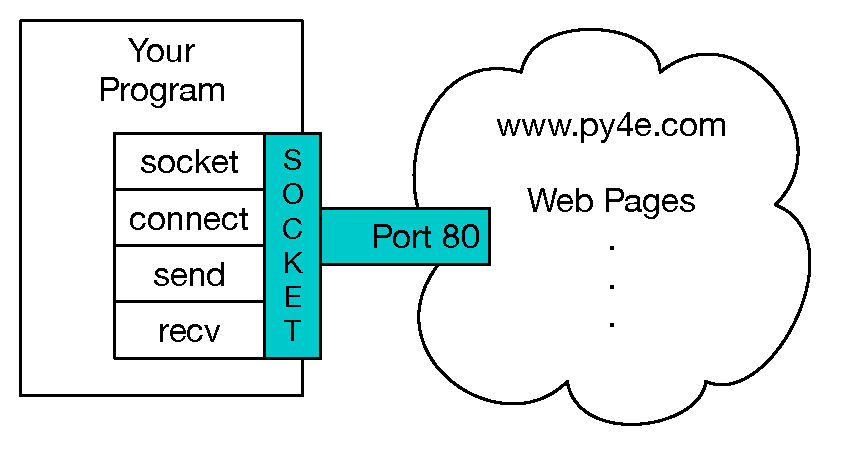
\includegraphics[keepaspectratio,alt={A Socket Connection},height=2.0in]{../images/socket.eps}}
\caption{A Socket Connection}
\end{figure}

Kapag naipadala na natin ang blank line na iyon, sumusulat tayo ng loop
na tumatanggap ng data sa 512-character chunks mula sa socket at
nagpi-print ng data hanggang wala nang data na mababasa (i.e., ang
recv() ay nagre-return ng empty string).

Ang program ay gumagawa ng sumusunod na output:

{\small
\begin{verbatim}
HTTP/1.1 200 OK
Date: Wed, 11 Apr 2018 18:52:55 GMT
Server: Apache/2.4.7 (Ubuntu)
Last-Modified: Sat, 13 May 2017 11:22:22 GMT
ETag: "a7-54f6609245537"
Accept-Ranges: bytes
Content-Length: 167
Cache-Control: max-age=0, no-cache, no-store, must-revalidate
Pragma: no-cache
Expires: Wed, 11 Jan 1984 05:00:00 GMT
Connection: close
Content-Type: text/plain

But soft what light through yonder window breaks
It is the east and Juliet is the sun
Arise fair sun and kill the envious moon
Who is already sick and pale with grief
\end{verbatim}
}

Ang output ay nagsisimula sa headers na ipinapadala ng web server para
ilarawan ang dokumento. Halimbawa, ang \texttt{Content-Type} header ay
nagpapahiwatig na ang dokumento ay plain text document
(\texttt{text/plain}).

Pagkatapos ipadala sa atin ng server ang headers, nagdaragdag ito ng
blank line para ipahiwatig ang dulo ng headers, at pagkatapos
nagpapadala ng aktwal na data ng file \emph{romeo.txt}.

Ang halimbawang ito ay nagpapakita kung paano gumawa ng low-level
network connection gamit ang sockets. Ang sockets ay maaaring gamitin
para makipag-communicate sa web server o sa mail server o marami pang
ibang uri ng servers. Ang kailangan lang ay hanapin ang dokumento na
naglalarawan sa protocol at sumulat ng code para magpadala at tumanggap
ng data ayon sa protocol.

Gayunpaman, dahil ang protocol na pinakakaraniwang ginagamit natin ay
ang HTTP web protocol, ang Python ay may espesyal na library na
partikular na idinisenyo para suportahan ang HTTP protocol para sa
pagkuha ng mga dokumento at data sa web.

Isa sa mga requirements para gamitin ang HTTP protocol ay ang
pangangailangan na magpadala at tumanggap ng data bilang bytes objects,
sa halip na strings. Sa naunang halimbawa, ang \texttt{encode()} at
\texttt{decode()} methods ay nagko-convert ng strings sa bytes objects
at pabalik.

Ang susunod na halimbawa ay gumagamit ng
\texttt{b\textquotesingle{}\textquotesingle{}} notation para tukuyin na
ang variable ay dapat i-store bilang bytes object. Ang \texttt{encode()}
at \texttt{b\textquotesingle{}\textquotesingle{}} ay katumbas.

{\small
\begin{verbatim}
>>> b'Hello world'
b'Hello world'
>>> 'Hello world'.encode()
b'Hello world'
\end{verbatim}
}

\section{Retrieving an image over
HTTP}\label{retrieving-an-image-over-http}

\index{urllib!image} \index{image!jpg} \index{jpg}

Sa halimbawa sa itaas, kumuha tayo ng plain text file na may newlines sa
file at simpleng kinopya ang data sa screen habang tumatakbo ang
program. Maaari tayong gumamit ng katulad na program para kumuha ng
image gamit ang HTTP. Sa halip na kopyahin ang data sa screen habang
tumatakbo ang program, ina-accumulate natin ang data sa string,
tinatanggal ang headers, at pagkatapos sinasave ang image data sa file
tulad ng sumusunod:

\begin{Shaded}
\begin{Highlighting}[]
\ImportTok{import}\NormalTok{ socket}
\ImportTok{import}\NormalTok{ time}

\NormalTok{HOST }\OperatorTok{=} \StringTok{\textquotesingle{}data.pr4e.org\textquotesingle{}}
\NormalTok{PORT }\OperatorTok{=} \DecValTok{80}
\NormalTok{mysock }\OperatorTok{=}\NormalTok{ socket.socket(socket.AF\_INET, socket.SOCK\_STREAM)}
\NormalTok{mysock.}\ExtensionTok{connect}\NormalTok{((HOST, PORT))}
\NormalTok{mysock.sendall(}\StringTok{b\textquotesingle{}GET http://data.pr4e.org/cover3.jpg HTTP/1.0}\CharTok{\textbackslash{}r\textbackslash{}n\textbackslash{}r\textbackslash{}n}\StringTok{\textquotesingle{}}\NormalTok{)}
\NormalTok{count }\OperatorTok{=} \DecValTok{0}
\NormalTok{picture }\OperatorTok{=} \StringTok{b""}

\ControlFlowTok{while} \VariableTok{True}\NormalTok{:}
\NormalTok{    data }\OperatorTok{=}\NormalTok{ mysock.recv(}\DecValTok{5120}\NormalTok{)}
    \ControlFlowTok{if} \BuiltInTok{len}\NormalTok{(data) }\OperatorTok{\textless{}} \DecValTok{1}\NormalTok{: }\ControlFlowTok{break}
    \CommentTok{\#time.sleep(0.25)}
\NormalTok{    count }\OperatorTok{=}\NormalTok{ count }\OperatorTok{+} \BuiltInTok{len}\NormalTok{(data)}
    \BuiltInTok{print}\NormalTok{(}\BuiltInTok{len}\NormalTok{(data), count)}
\NormalTok{    picture }\OperatorTok{=}\NormalTok{ picture }\OperatorTok{+}\NormalTok{ data}

\NormalTok{mysock.close()}

\CommentTok{\# Look for the end of the header (2 CRLF)}
\NormalTok{pos }\OperatorTok{=}\NormalTok{ picture.find(}\StringTok{b"}\CharTok{\textbackslash{}r\textbackslash{}n\textbackslash{}r\textbackslash{}n}\StringTok{"}\NormalTok{)}
\BuiltInTok{print}\NormalTok{(}\StringTok{\textquotesingle{}Header length\textquotesingle{}}\NormalTok{, pos)}
\BuiltInTok{print}\NormalTok{(picture[:pos].decode())}

\CommentTok{\# Skip past the header and save the picture data}
\NormalTok{picture }\OperatorTok{=}\NormalTok{ picture[pos}\OperatorTok{+}\DecValTok{4}\NormalTok{:]}
\NormalTok{fhand }\OperatorTok{=} \BuiltInTok{open}\NormalTok{(}\StringTok{"stuff.jpg"}\NormalTok{, }\StringTok{"wb"}\NormalTok{)}
\NormalTok{fhand.write(picture)}
\NormalTok{fhand.close()}

\CommentTok{\# Code: https://www.py4e.com/code3/urljpeg.py}
\end{Highlighting}
\end{Shaded}

Kapag tumatakbo ang program, gumagawa ito ng sumusunod na output:

{\small
\begin{verbatim}
$ python urljpeg.py
5120 5120
5120 10240
4240 14480
5120 19600
...
5120 214000
3200 217200
5120 222320
5120 227440
3167 230607
Header length 393
HTTP/1.1 200 OK
Date: Wed, 11 Apr 2018 18:54:09 GMT
Server: Apache/2.4.7 (Ubuntu)
Last-Modified: Mon, 15 May 2017 12:27:40 GMT
ETag: "38342-54f8f2e5b6277"
Accept-Ranges: bytes
Content-Length: 230210
Vary: Accept-Encoding
Cache-Control: max-age=0, no-cache, no-store, must-revalidate
Pragma: no-cache
Expires: Wed, 11 Jan 1984 05:00:00 GMT
Connection: close
Content-Type: image/jpeg
\end{verbatim}
}

Makikita mo na para sa url na ito, ang \texttt{Content-Type} header ay
nagpapahiwatig na ang body ng dokumento ay image (\texttt{image/jpeg}).
Kapag natapos na ang program, maaari mong tingnan ang image data sa
pamamagitan ng pagbubukas ng file na \texttt{stuff.jpg} sa image viewer.

Habang tumatakbo ang program, makikita mo na hindi tayo nakakakuha ng
5120 characters sa bawat pagkakataon na tinatawag natin ang
\texttt{recv()} method. Nakakakuha tayo ng kasing dami ng characters na
na-transfer sa network sa atin ng web server sa sandaling tinatawag
natin ang \texttt{recv()}. Sa halimbawang ito, nakakakuha tayo ng kasing
kaunti ng 3200 characters sa bawat pagkakataon na humihingi tayo ng
hanggang 5120 characters ng data.

Ang iyong results ay maaaring magkaiba depende sa network speed mo.
Tandaan din na sa huling tawag sa \texttt{recv()} nakakakuha tayo ng
3167 bytes, na siyang dulo ng stream, at sa susunod na tawag sa
\texttt{recv()} nakakakuha tayo ng zero-length string na nagsasabi sa
atin na ang server ay tumawag na sa \texttt{close()} sa dulo nito ng
socket at wala nang data na darating.

\index{time} \index{time.sleep}

Maaari nating pabagalin ang sunud-sunod na \texttt{recv()} calls natin
sa pamamagitan ng pag-uncomment sa tawag sa \texttt{time.sleep()}. Sa
ganitong paraan, naghihintay tayo ng quarter ng segundo pagkatapos ng
bawat tawag para makakuha ng ``lead'' ang server at magpadala ng mas
maraming data sa atin bago tayo tumawag ulit sa \texttt{recv()}. Sa
delay, sa lugar ang program ay nag-e-execute tulad ng sumusunod:

{\small
\begin{verbatim}
$ python urljpeg.py
5120 5120
5120 10240
5120 15360
...
5120 225280
5120 230400
207 230607
Header length 393
HTTP/1.1 200 OK
Date: Wed, 11 Apr 2018 21:42:08 GMT
Server: Apache/2.4.7 (Ubuntu)
Last-Modified: Mon, 15 May 2017 12:27:40 GMT
ETag: "38342-54f8f2e5b6277"
Accept-Ranges: bytes
Content-Length: 230210
Vary: Accept-Encoding
Cache-Control: max-age=0, no-cache, no-store, must-revalidate
Pragma: no-cache
Expires: Wed, 11 Jan 1984 05:00:00 GMT
Connection: close
Content-Type: image/jpeg
\end{verbatim}
}

Ngayon maliban sa una at huling tawag sa \texttt{recv()}, nakakakuha na
tayo ng 5120 characters sa bawat pagkakataon na humihingi tayo ng bagong
data.

Mayroong buffer sa pagitan ng server na gumagawa ng \texttt{send()}
requests at application natin na gumagawa ng \texttt{recv()} requests.
Kapag pinatakbo natin ang program na may delay sa lugar, sa ilang punto
ang server ay maaaring mapuno ang buffer sa socket at mapilit na
mag-pause hanggang magsimulang mag-emptying ng buffer ang program natin.
Ang pag-pause ng alinman sa sending application o receiving application
ay tinatawag na ``flow control.''

\index{flow control}

\section{\texorpdfstring{Retrieving web pages with
\texttt{urllib}}{Retrieving web pages with urllib}}\label{retrieving-web-pages-with-urllib}

Habang maaari nating manu-manong magpadala at tumanggap ng data sa HTTP
gamit ang socket library, mayroong mas simpleng paraan para gawin ang
karaniwang gawaing ito sa Python sa pamamagitan ng paggamit ng
\texttt{urllib} library.

Gamit ang \texttt{urllib}, maaari mong tratuhin ang web page na parang
file. Simpleng ipinapahiwatig mo lang kung aling web page ang gusto mong
kunin at ang \texttt{urllib} ay nagha-handle ng lahat ng HTTP protocol
at header details.

Ang katumbas na code para basahin ang \emph{romeo.txt} file mula sa web
gamit ang \texttt{urllib} ay ganito:

\begin{Shaded}
\begin{Highlighting}[]
\ImportTok{import}\NormalTok{ urllib.request}

\NormalTok{fhand }\OperatorTok{=}\NormalTok{ urllib.request.urlopen(}\StringTok{\textquotesingle{}http://data.pr4e.org/romeo.txt\textquotesingle{}}\NormalTok{)}
\ControlFlowTok{for}\NormalTok{ line }\KeywordTok{in}\NormalTok{ fhand:}
    \BuiltInTok{print}\NormalTok{(line.decode().strip())}

\CommentTok{\# Code: https://www.py4e.com/code3/urllib1.py}
\end{Highlighting}
\end{Shaded}

Kapag nabuksan na ang web page gamit ang
\texttt{urllib.request.urlopen}, maaari nating tratuhin ito na parang
file at basahin ito gamit ang \texttt{for} loop.

Kapag tumatakbo ang program, nakikita lang natin ang output ng contents
ng file. Ang headers ay ipinapadala pa rin, pero ang \texttt{urllib}
code ay kumukonsumo ng headers at nagre-return lang ng data sa atin.

{\small
\begin{verbatim}
But soft what light through yonder window breaks
It is the east and Juliet is the sun
Arise fair sun and kill the envious moon
Who is already sick and pale with grief
\end{verbatim}
}

Bilang halimbawa, maaari tayong sumulat ng program para kunin ang data
para sa \texttt{romeo.txt} at i-compute ang frequency ng bawat salita sa
file tulad ng sumusunod:

\begin{Shaded}
\begin{Highlighting}[]
\ImportTok{import}\NormalTok{ urllib.request, urllib.parse, urllib.error}

\NormalTok{fhand }\OperatorTok{=}\NormalTok{ urllib.request.urlopen(}\StringTok{\textquotesingle{}http://data.pr4e.org/romeo.txt\textquotesingle{}}\NormalTok{)}

\NormalTok{counts }\OperatorTok{=} \BuiltInTok{dict}\NormalTok{()}
\ControlFlowTok{for}\NormalTok{ line }\KeywordTok{in}\NormalTok{ fhand:}
\NormalTok{    words }\OperatorTok{=}\NormalTok{ line.decode().split()}
    \ControlFlowTok{for}\NormalTok{ word }\KeywordTok{in}\NormalTok{ words:}
\NormalTok{        counts[word] }\OperatorTok{=}\NormalTok{ counts.get(word, }\DecValTok{0}\NormalTok{) }\OperatorTok{+} \DecValTok{1}
\BuiltInTok{print}\NormalTok{(counts)}

\CommentTok{\# Code: https://www.py4e.com/code3/urlwords.py}
\end{Highlighting}
\end{Shaded}

Muli, kapag nabuksan na natin ang web page, maaari nating basahin ito na
parang local file.

\section{\texorpdfstring{Reading binary files using
\texttt{urllib}}{Reading binary files using urllib}}\label{reading-binary-files-using-urllib}

Minsan gusto mong kunin ang non-text (o binary) file tulad ng image o
video file. Ang data sa mga files na ito ay karaniwang hindi
kapaki-pakinabang na i-print, pero madali mong magagawa ng kopya ng URL
sa local file sa hard disk mo gamit ang \texttt{urllib}.

\index{binary file}

Ang pattern ay buksan ang URL at gamitin ang \texttt{read} para
i-download ang buong contents ng dokumento sa string variable
(\texttt{img}) pagkatapos isulat ang impormasyong iyon sa local file
tulad ng sumusunod:

\begin{Shaded}
\begin{Highlighting}[]
\ImportTok{import}\NormalTok{ urllib.request, urllib.parse, urllib.error}

\NormalTok{img }\OperatorTok{=}\NormalTok{ urllib.request.urlopen(}\StringTok{\textquotesingle{}http://data.pr4e.org/cover3.jpg\textquotesingle{}}\NormalTok{).read()}
\NormalTok{fhand }\OperatorTok{=} \BuiltInTok{open}\NormalTok{(}\StringTok{\textquotesingle{}cover3.jpg\textquotesingle{}}\NormalTok{, }\StringTok{\textquotesingle{}wb\textquotesingle{}}\NormalTok{)}
\NormalTok{fhand.write(img)}
\NormalTok{fhand.close()}

\CommentTok{\# Code: https://www.py4e.com/code3/curl1.py}
\end{Highlighting}
\end{Shaded}

Ang program na ito ay nagbabasa ng lahat ng data nang sabay-sabay sa
network at nag-i-store nito sa variable na \texttt{img} sa main memory
ng iyong computer, pagkatapos binubuksan ang file na \texttt{cover.jpg}
at isinusulat ang data sa disk mo. Ang \texttt{wb} argument para sa
\texttt{open()} ay nagbubukas ng binary file para sa pagsusulat lang.
Ang program na ito ay gagana kung ang laki ng file ay mas maliit kaysa
sa laki ng memory ng computer mo.

Gayunpaman kung ito ay malaking audio o video file, ang program na ito
ay maaaring mag-crash o hindi bababa ay tumakbo nang napakabagal kapag
naubusan ng memory ang computer mo. Para maiwasan ang pagkaubos ng
memory, kinukuha natin ang data sa blocks (o buffers) at pagkatapos
isinusulat ang bawat block sa disk mo bago kunin ang susunod na block.
Sa ganitong paraan ang program ay maaaring magbasa ng anumang laking
file nang hindi ginagamit ang lahat ng memory na mayroon ka sa computer
mo.

\begin{Shaded}
\begin{Highlighting}[]
\ImportTok{import}\NormalTok{ urllib.request, urllib.parse, urllib.error}

\NormalTok{img }\OperatorTok{=}\NormalTok{ urllib.request.urlopen(}\StringTok{\textquotesingle{}http://data.pr4e.org/cover3.jpg\textquotesingle{}}\NormalTok{)}
\NormalTok{fhand }\OperatorTok{=} \BuiltInTok{open}\NormalTok{(}\StringTok{\textquotesingle{}cover3.jpg\textquotesingle{}}\NormalTok{, }\StringTok{\textquotesingle{}wb\textquotesingle{}}\NormalTok{)}
\NormalTok{size }\OperatorTok{=} \DecValTok{0}
\ControlFlowTok{while} \VariableTok{True}\NormalTok{:}
\NormalTok{    info }\OperatorTok{=}\NormalTok{ img.read(}\DecValTok{100000}\NormalTok{)}
    \ControlFlowTok{if} \BuiltInTok{len}\NormalTok{(info) }\OperatorTok{\textless{}} \DecValTok{1}\NormalTok{: }\ControlFlowTok{break}
\NormalTok{    size }\OperatorTok{=}\NormalTok{ size }\OperatorTok{+} \BuiltInTok{len}\NormalTok{(info)}
\NormalTok{    fhand.write(info)}

\BuiltInTok{print}\NormalTok{(size, }\StringTok{\textquotesingle{}characters copied.\textquotesingle{}}\NormalTok{)}
\NormalTok{fhand.close()}

\CommentTok{\# Code: https://www.py4e.com/code3/curl2.py}
\end{Highlighting}
\end{Shaded}

Sa halimbawang ito, nagbabasa lang tayo ng 100,000 characters sa isang
pagkakataon at pagkatapos isinusulat ang mga characters na iyon sa file
na \texttt{cover3.jpg} bago kunin ang susunod na 100,000 characters ng
data mula sa web.

Ang program na ito ay tumatakbo tulad ng sumusunod:

{\small
\begin{verbatim}
python curl2.py
230210 characters copied.
\end{verbatim}
}

\section{Parsing HTML and scraping the
web}\label{parsing-html-and-scraping-the-web}

\index{web!scraping} \index{parsing HTML}

Isa sa karaniwang gamit ng \texttt{urllib} capability sa Python ay
\emph{i-scrape} ang web. Ang web scraping ay kapag sumusulat tayo ng
program na nagpapanggap bilang web browser at kumukuha ng pages,
pagkatapos sinusuri ang data sa mga pages na iyon na naghahanap ng
patterns.

Bilang halimbawa, ang search engine tulad ng Google ay titingnan ang
source ng isang web page at kukunin ang links sa iba pang pages at
kukunin ang mga pages na iyon, kumukuha ng links, at iba pa. Gamit ang
technique na ito, ang Google ay \emph{nag-spider} sa halos lahat ng
pages sa web.

Gumagamit din ang Google ng frequency ng links mula sa pages na nakikita
nito patungo sa partikular na page bilang isang sukat kung gaano
``important'' ang page at kung gaano kataas dapat lumabas ang page sa
search results nito.

\section{Parsing HTML using regular
expressions}\label{parsing-html-using-regular-expressions}

Ang isang simpleng paraan para mag-parse ng HTML ay gumamit ng regular
expressions para paulit-ulit na maghanap at kunin ang substrings na
tumutugma sa partikular na pattern.

Narito ang simpleng web page:

\begin{Shaded}
\begin{Highlighting}[]
\DataTypeTok{\textless{}}\KeywordTok{h1}\DataTypeTok{\textgreater{}}\NormalTok{The First Page}\DataTypeTok{\textless{}/}\KeywordTok{h1}\DataTypeTok{\textgreater{}}
\DataTypeTok{\textless{}}\KeywordTok{p}\DataTypeTok{\textgreater{}}
\NormalTok{If you like, you can switch to the}
\DataTypeTok{\textless{}}\KeywordTok{a}\OtherTok{ href}\OperatorTok{=}\StringTok{"http://www.dr{-}chuck.com/page2.htm"}\DataTypeTok{\textgreater{}}
\NormalTok{Second Page}\DataTypeTok{\textless{}/}\KeywordTok{a}\DataTypeTok{\textgreater{}}\NormalTok{.}
\DataTypeTok{\textless{}/}\KeywordTok{p}\DataTypeTok{\textgreater{}}
\end{Highlighting}
\end{Shaded}

Maaari tayong gumawa ng well-formed regular expression para tumugma at
kunin ang link values mula sa text sa itaas tulad ng sumusunod:

{\small
\begin{verbatim}
href="http[s]?://.+?"
\end{verbatim}
}

Ang regular expression natin ay naghahanap ng strings na nagsisimula sa
``href="http://'' o ``href="https://'', na sinusundan ng isa o higit
pang characters (\texttt{.+?}), na sinusundan ng isa pang double quote.
Ang question mark sa likod ng \texttt{{[}s{]}?} ay nagpapahiwatig na
maghanap ng string na ``http'' na sinusundan ng zero o isang ``s''.

Ang question mark na idinagdag sa \texttt{.+?} ay nagpapahiwatig na ang
match ay dapat gawin sa ``non-greedy'' fashion sa halip na ``greedy''
fashion. Ang non-greedy match ay sinusubukang hanapin ang
\emph{pinakamaliit} na posibleng matching string at ang greedy match ay
sinusubukang hanapin ang \emph{pinakamalaki} na posibleng matching
string.

\index{greedy} \index{non-greedy}

Nagdaragdag tayo ng parentheses sa regular expression natin para
ipahiwatig kung aling parte ng matched string natin ang gusto nating
kunin, at gumagawa ng sumusunod na program:

\index{regex!parentheses} \index{parentheses!regular expression}

\begin{Shaded}
\begin{Highlighting}[]
\CommentTok{\# Search for link values within URL input}
\ImportTok{import}\NormalTok{ urllib.request, urllib.parse, urllib.error}
\ImportTok{import}\NormalTok{ re}
\ImportTok{import}\NormalTok{ ssl}

\CommentTok{\# Ignore SSL certificate errors}
\NormalTok{ctx }\OperatorTok{=}\NormalTok{ ssl.create\_default\_context()}
\NormalTok{ctx.check\_hostname }\OperatorTok{=} \VariableTok{False}
\NormalTok{ctx.verify\_mode }\OperatorTok{=}\NormalTok{ ssl.CERT\_NONE}

\NormalTok{url }\OperatorTok{=} \BuiltInTok{input}\NormalTok{(}\StringTok{\textquotesingle{}Enter {-} \textquotesingle{}}\NormalTok{)}
\NormalTok{html }\OperatorTok{=}\NormalTok{ urllib.request.urlopen(url, context}\OperatorTok{=}\NormalTok{ctx).read()}
\NormalTok{links }\OperatorTok{=}\NormalTok{ re.findall(}\StringTok{b\textquotesingle{}href="(http[s]?://.*?)"\textquotesingle{}}\NormalTok{, html)}
\ControlFlowTok{for}\NormalTok{ link }\KeywordTok{in}\NormalTok{ links:}
    \BuiltInTok{print}\NormalTok{(link.decode())}

\CommentTok{\# Code: https://www.py4e.com/code3/urlregex.py}
\end{Highlighting}
\end{Shaded}

Ang \texttt{ssl} library ay nagpapahintulot sa program na ito na
ma-access ang web sites na mahigpit na nagpapatupad ng HTTPS. Ang
\texttt{read} method ay nagre-return ng HTML source code bilang bytes
object sa halip na mag-return ng HTTPResponse object. Ang
\texttt{findall} regular expression method ay magbibigay sa atin ng list
ng lahat ng strings na tumutugma sa aming regular expression, na
nagre-return lang ng link text sa pagitan ng double quotes.

Kapag pinatakbo natin ang program at nag-input ng URL, makukuha natin
ang sumusunod na output:

{\small
\begin{verbatim}
Enter - https://docs.python.org
https://docs.python.org/3/index.html
https://www.python.org/
https://docs.python.org/3.8/
https://docs.python.org/3.7/
https://docs.python.org/3.5/
https://docs.python.org/2.7/
https://www.python.org/doc/versions/
https://www.python.org/dev/peps/
https://wiki.python.org/moin/BeginnersGuide
https://wiki.python.org/moin/PythonBooks
https://www.python.org/doc/av/
https://www.python.org/
https://www.python.org/psf/donations/
http://sphinx.pocoo.org/
\end{verbatim}
}

Ang regular expressions ay gumagana nang napakaganda kapag ang HTML mo
ay well formatted at predictable. Pero dahil mayroong maraming
``broken'' HTML pages doon, ang solusyon na gumagamit lang ng regular
expressions ay maaaring makaligtaan ang ilang valid links o magtapos sa
masamang data.

Maaari itong malutas sa pamamagitan ng paggamit ng robust HTML parsing
library.

\section{Parsing HTML using
BeautifulSoup}\label{parsing-html-using-beautifulsoup}

\index{BeautifulSoup}

Kahit na ang HTML ay mukhang XML\footnote{Ang XML format ay inilarawan
  sa susunod na chapter.} at ang ilang pages ay maingat na ginawa para
maging XML, karamihan ng HTML ay karaniwang sira sa mga paraan na
nagdudulot na ang XML parser ay tumanggi sa buong page ng HTML bilang
hindi wastong format.

Mayroong ilang Python libraries na maaaring tumulong sa iyo na mag-parse
ng HTML at kumuha ng data mula sa pages. Ang bawat library ay may
sariling strengths at weaknesses at maaari kang pumili ng isa batay sa
iyong pangangailangan.

Bilang halimbawa, simpleng magpa-parse tayo ng ilang HTML input at
kumuha ng links gamit ang \emph{BeautifulSoup} library. Ang
BeautifulSoup ay nagpaparaya sa lubhang flawed HTML at nagpapahintulot
pa rin sa iyo na madaling kunin ang data na kailangan mo. Maaari mong
i-download at i-install ang BeautifulSoup code mula sa:

\url{https://pypi.python.org/pypi/beautifulsoup4}

Ang impormasyon tungkol sa pag-install ng BeautifulSoup gamit ang Python
Package Index tool na \texttt{pip} ay available sa:

\url{https://packaging.python.org/tutorials/installing-packages/}

Gagamitin natin ang \texttt{urllib} para basahin ang page at pagkatapos
gamitin ang \texttt{BeautifulSoup} para kunin ang \texttt{href}
attributes mula sa anchor (\texttt{a}) tags.

\index{BeautifulSoup} \index{HTML} \index{parsing!HTML}

\begin{Shaded}
\begin{Highlighting}[]
\CommentTok{\# To run this, download the BeautifulSoup zip file}
\CommentTok{\# http://www.py4e.com/code3/bs4.zip}
\CommentTok{\# or pip install beautifulsoup4 to ensure you have the latest version}
\CommentTok{\# and unzip it in the same directory as this file}

\ImportTok{import}\NormalTok{ urllib.request, urllib.parse, urllib.error}
\ImportTok{from}\NormalTok{ bs4 }\ImportTok{import}\NormalTok{ BeautifulSoup}
\ImportTok{import}\NormalTok{ ssl }\CommentTok{\# defauts to certicate verification and most secure protocol (now TLS)}

\CommentTok{\# Ignore SSL/TLS certificate errors}
\NormalTok{ctx }\OperatorTok{=}\NormalTok{ ssl.create\_default\_context()}
\NormalTok{ctx.check\_hostname }\OperatorTok{=} \VariableTok{False}
\NormalTok{ctx.verify\_mode }\OperatorTok{=}\NormalTok{ ssl.CERT\_NONE}

\NormalTok{url }\OperatorTok{=} \BuiltInTok{input}\NormalTok{(}\StringTok{\textquotesingle{}Enter {-} \textquotesingle{}}\NormalTok{)}
\NormalTok{html }\OperatorTok{=}\NormalTok{ urllib.request.urlopen(url, context}\OperatorTok{=}\NormalTok{ctx).read()}
\NormalTok{soup }\OperatorTok{=}\NormalTok{ BeautifulSoup(html, }\StringTok{\textquotesingle{}html.parser\textquotesingle{}}\NormalTok{)}

\CommentTok{\# Retrieve all of the anchor tags}
\NormalTok{tags }\OperatorTok{=}\NormalTok{ soup(}\StringTok{\textquotesingle{}a\textquotesingle{}}\NormalTok{)}
\ControlFlowTok{for}\NormalTok{ tag }\KeywordTok{in}\NormalTok{ tags:}
    \BuiltInTok{print}\NormalTok{(tag.get(}\StringTok{\textquotesingle{}href\textquotesingle{}}\NormalTok{, }\VariableTok{None}\NormalTok{))}

\CommentTok{\# Code: https://www.py4e.com/code3/urllinks.py}
\end{Highlighting}
\end{Shaded}

Ang program ay nagpo-prompt para sa web address, pagkatapos binubuksan
ang web page, binabasa ang data at ipinapasa ang data sa BeautifulSoup
parser, at pagkatapos kumukuha ng lahat ng anchor tags at nagpi-print ng
\texttt{href} attribute para sa bawat tag.

Kapag tumatakbo ang program, gumagawa ito ng sumusunod na output:

{\small
\begin{verbatim}
Enter - https://docs.python.org
genindex.html
py-modindex.html
https://www.python.org/
#
whatsnew/3.6.html
whatsnew/index.html
tutorial/index.html
library/index.html
reference/index.html
using/index.html
howto/index.html
installing/index.html
distributing/index.html
extending/index.html
c-api/index.html
faq/index.html
py-modindex.html
genindex.html
glossary.html
search.html
contents.html
bugs.html
about.html
license.html
copyright.html
download.html
https://docs.python.org/3.8/
https://docs.python.org/3.7/
https://docs.python.org/3.5/
https://docs.python.org/2.7/
https://www.python.org/doc/versions/
https://www.python.org/dev/peps/
https://wiki.python.org/moin/BeginnersGuide
https://wiki.python.org/moin/PythonBooks
https://www.python.org/doc/av/
genindex.html
py-modindex.html
https://www.python.org/
#
copyright.html
https://www.python.org/psf/donations/
bugs.html
http://sphinx.pocoo.org/
\end{verbatim}
}

Ang list na ito ay mas mahaba dahil ang ilang HTML anchor tags ay
relative paths (hal., tutorial/index.html) o in-page references (hal.,
`\#') na hindi kasama ang ``http://'' o ``https://'', na siyang
requirement sa regular expression natin.

Maaari mo ring gamitin ang BeautifulSoup para kunin ang iba't ibang
parte ng bawat tag:

\begin{Shaded}
\begin{Highlighting}[]
\CommentTok{\# To run this, download the BeautifulSoup zip file}
\CommentTok{\# http://www.py4e.com/code3/bs4.zip}
\CommentTok{\# and unzip it in the same directory as this file}

\ImportTok{from}\NormalTok{ urllib.request }\ImportTok{import}\NormalTok{ urlopen}
\ImportTok{from}\NormalTok{ bs4 }\ImportTok{import}\NormalTok{ BeautifulSoup}
\ImportTok{import}\NormalTok{ ssl}

\CommentTok{\# Ignore SSL certificate errors}
\NormalTok{ctx }\OperatorTok{=}\NormalTok{ ssl.create\_default\_context()}
\NormalTok{ctx.check\_hostname }\OperatorTok{=} \VariableTok{False}
\NormalTok{ctx.verify\_mode }\OperatorTok{=}\NormalTok{ ssl.CERT\_NONE}

\NormalTok{url }\OperatorTok{=} \BuiltInTok{input}\NormalTok{(}\StringTok{\textquotesingle{}Enter {-} \textquotesingle{}}\NormalTok{)}
\NormalTok{html }\OperatorTok{=}\NormalTok{ urlopen(url, context}\OperatorTok{=}\NormalTok{ctx).read()}
\NormalTok{soup }\OperatorTok{=}\NormalTok{ BeautifulSoup(html, }\StringTok{"html.parser"}\NormalTok{)}

\CommentTok{\# Retrieve all of the anchor tags}
\NormalTok{tags }\OperatorTok{=}\NormalTok{ soup(}\StringTok{\textquotesingle{}a\textquotesingle{}}\NormalTok{)}
\ControlFlowTok{for}\NormalTok{ tag }\KeywordTok{in}\NormalTok{ tags:}
    \CommentTok{\# Look at the parts of a tag}
    \BuiltInTok{print}\NormalTok{(}\StringTok{\textquotesingle{}TAG:\textquotesingle{}}\NormalTok{, tag)}
    \BuiltInTok{print}\NormalTok{(}\StringTok{\textquotesingle{}URL:\textquotesingle{}}\NormalTok{, tag.get(}\StringTok{\textquotesingle{}href\textquotesingle{}}\NormalTok{, }\VariableTok{None}\NormalTok{))}
    \BuiltInTok{print}\NormalTok{(}\StringTok{\textquotesingle{}Contents:\textquotesingle{}}\NormalTok{, tag.contents[}\DecValTok{0}\NormalTok{])}
    \BuiltInTok{print}\NormalTok{(}\StringTok{\textquotesingle{}Attrs:\textquotesingle{}}\NormalTok{, tag.attrs)}

\CommentTok{\# Code: https://www.py4e.com/code3/urllink2.py}
\end{Highlighting}
\end{Shaded}

{\small
\begin{verbatim}
python urllink2.py
Enter - http://www.dr-chuck.com/page1.htm
TAG: <a href="http://www.dr-chuck.com/page2.htm">
Second Page</a>
URL: http://www.dr-chuck.com/page2.htm
Content: ['\nSecond Page']
Attrs: [('href', 'http://www.dr-chuck.com/page2.htm')]
\end{verbatim}
}

Ang \texttt{html.parser} ay ang HTML parser na kasama sa standard Python
3 library. Ang impormasyon tungkol sa iba pang HTML parsers ay available
sa:

\url{http://www.crummy.com/software/BeautifulSoup/bs4/doc/\#installing-a-parser}

Ang mga halimbawang ito ay nagsisimula lang na ipakita ang kapangyarihan
ng BeautifulSoup pagdating sa pag-parse ng HTML.

\section{Bonus section for Unix / Linux
users}\label{bonus-section-for-unix-linux-users-1}

Kung mayroon kang Linux, Unix, o Macintosh computer, malamang mayroon
kang commands na naka-build sa operating system mo na kumukuha ng
parehong plain text at binary files gamit ang HTTP o File Transfer (FTP)
protocols. Isa sa mga commands na ito ay \texttt{curl}:

\index{curl}

\begin{Shaded}
\begin{Highlighting}[]
\ExtensionTok{$}\NormalTok{ curl }\AttributeTok{{-}O}\NormalTok{ http://www.py4e.com/cover.jpg}
\end{Highlighting}
\end{Shaded}

Ang command na \texttt{curl} ay maikli para sa ``copy URL'' at kaya ang
dalawang halimbawa na nakalista kanina para kumuha ng binary files gamit
ang \texttt{urllib} ay matalinong pinangalanan na \texttt{curl1.py} at
\texttt{curl2.py} sa
\href{http://www.py4e.com/code3}{www.py4e.com/code3} dahil
nag-i-implement sila ng katulad na functionality sa \texttt{curl}
command. Mayroon ding \texttt{curl3.py} sample program na gumagawa ng
gawaing ito nang mas epektibo, kung sakaling gusto mong talagang gamitin
ang pattern na ito sa program na sinusulat mo.

Ang pangalawang command na gumagana nang katulad ay \texttt{wget}:

\index{wget}

\begin{Shaded}
\begin{Highlighting}[]
\ExtensionTok{$}\NormalTok{ wget http://www.py4e.com/cover.jpg}
\end{Highlighting}
\end{Shaded}

Pareho sa mga commands na ito ay nagpapasimple sa pagkuha ng webpages at
remote files.

\section{Glossary}\label{glossary-11}

\begin{description}
\tightlist
\item[BeautifulSoup]
Python library para sa pag-parse ng HTML documents at pagkuha ng data
mula sa HTML documents na nagko-compensate para sa karamihan ng
imperfections sa HTML na karaniwang hindi pinapansin ng browsers. Maaari
mong i-download ang BeautifulSoup code mula sa
\href{http://www.crummy.com}{www.crummy.com}. \index{BeautifulSoup}
\item[port]
Numero na karaniwang nagpapahiwatig kung aling application ang
kinokontak mo kapag gumagawa ka ng socket connection sa server. Bilang
halimbawa, ang web traffic ay karaniwang gumagamit ng port 80 habang ang
email traffic ay gumagamit ng port 25. \index{port}
\item[scrape]
Kapag ang program ay nagpapanggap bilang web browser at kumukuha ng web
page, pagkatapos tumitingin sa web page content. Kadalasan ang mga
programs ay sumusunod sa links sa isang page para hanapin ang susunod na
page para maaari nilang dumaan sa network ng pages o social network.
\index{socket}
\item[socket]
Network connection sa pagitan ng dalawang applications kung saan ang
applications ay maaaring magpadala at tumanggap ng data sa alinmang
direksyon. \index{socket}
\item[spider]
Ang gawain ng web search engine na kumukuha ng page at pagkatapos lahat
ng pages na naka-link mula sa page at iba pa hanggang mayroon na silang
halos lahat ng pages sa Internet na ginagamit nila para gumawa ng search
index nila. \index{spider}
\end{description}

\section{Exercises}\label{exercises-11}

\textbf{Exercise 1:} Baguhin ang socket program na \texttt{socket1.py}
para mag-prompt sa user para sa URL para makabasa ito ng anumang web
page.

Maaari mong gamitin ang
\texttt{split(\textquotesingle{}/\textquotesingle{})} para hatiin ang
URL sa component parts nito para makakuha ka ng host name para sa socket
\texttt{connect} call. Magdagdag ng error checking gamit ang
\texttt{try} at \texttt{except} para ma-handle ang kondisyon kung saan
ang user ay nag-e-enter ng hindi wastong format o hindi umiiral na URL.

\textbf{Exercise 2:} Baguhin ang socket program mo para bilangin ang
bilang ng characters na natanggap nito at huminto sa pag-display ng
anumang text pagkatapos na ipakita ang 3000 characters. Ang program ay
dapat kumuha ng buong dokumento at bilangin ang kabuuang bilang ng
characters at ipakita ang bilang ng bilang ng characters sa dulo ng
dokumento.

\textbf{Exercise 3:} Gumamit ng \texttt{urllib} para i-replicate ang
naunang exercise ng (1) pagkuha ng dokumento mula sa URL, (2)
pag-display ng hanggang 3000 characters, at (3) pagbibilang ng kabuuang
bilang ng characters sa dokumento. Huwag mag-alala tungkol sa headers
para sa exercise na ito, simpleng ipakita ang unang 3000 characters ng
document contents.

\textbf{Exercise 4:} Baguhin ang \texttt{urllinks.py} program para kunin
at bilangin ang paragraph (p) tags mula sa retrieved HTML document at
ipakita ang bilang ng paragraphs bilang output ng program mo. Huwag
ipakita ang paragraph text, bilangin lang sila. I-test ang program mo sa
ilang maliliit na web pages pati na rin sa ilang mas malalaking web
pages.

\textbf{Exercise 5:} (Advanced) Baguhin ang socket program para ipakita
lang ang data pagkatapos matanggap ang headers at blank line. Tandaan na
ang \texttt{recv} ay tumatanggap ng characters (newlines at lahat),
hindi lines.

\chapter{Using Web Services}\label{using-web-services}

Nang naging madali na ang pagkuha ng documents at pag-parse ng documents
sa HTTP gamit ang programs, hindi nagtagal bago nabuo ang approach kung
saan nagsimula tayong gumawa ng documents na partikular na idinisenyo
para konsumahin ng iba pang programs (i.e., hindi HTML para ipakita sa
browser).

Mayroong dalawang karaniwang format na ginagamit natin kapag
nagpapalitan ng data sa web. Ang eXtensible Markup Language (XML) ay
ginagamit na ng napakatagal at pinakaangkop para sa pagpapalitan ng
document-style data. Kapag ang programs ay gusto lang magpalitan ng
dictionaries, lists, o iba pang internal impormasyon sa isa't isa,
gumagamit sila ng JavaScript Object Notation (JSON) (tingnan ang
\href{http://www.json.org}{www.json.org}). Titingnan natin ang parehong
format.

\section{eXtensible Markup Language -
XML}\label{extensible-markup-language---xml}

Ang XML ay mukhang katulad ng HTML, pero ang XML ay mas structured kaysa
sa HTML. Narito ang sample ng XML document:

\begin{Shaded}
\begin{Highlighting}[]
\NormalTok{\textless{}}\KeywordTok{person}\NormalTok{\textgreater{}}
\NormalTok{  \textless{}}\KeywordTok{name}\NormalTok{\textgreater{}Chuck\textless{}/}\KeywordTok{name}\NormalTok{\textgreater{}}
\NormalTok{  \textless{}}\KeywordTok{phone}\OtherTok{ type=}\StringTok{"intl"}\NormalTok{\textgreater{}}
\NormalTok{    +1 734 303 4456}
\NormalTok{  \textless{}/}\KeywordTok{phone}\NormalTok{\textgreater{}}
\NormalTok{  \textless{}}\KeywordTok{email}\OtherTok{ hide=}\StringTok{"yes"}\NormalTok{ /\textgreater{}}
\NormalTok{\textless{}/}\KeywordTok{person}\NormalTok{\textgreater{}}
\end{Highlighting}
\end{Shaded}

Ang bawat pares ng opening (hal.,
\texttt{\textless{}person\textgreater{}}) at closing tags (hal.,
\texttt{\textless{}/person\textgreater{}}) ay kumakatawan sa
\emph{element} o \emph{node} na may parehong pangalan sa tag (hal.,
\texttt{person}). Ang bawat element ay maaaring may ilang text, ilang
attributes (hal., \texttt{hide}), at iba pang nested elements. Kung ang
XML element ay empty (i.e., walang content), maaari itong ilarawan ng
self-closing tag (hal., \texttt{\textless{}email\ /\textgreater{}}).

Kadalasan kapaki-pakinabang na isipin ang XML document bilang tree
structure kung saan mayroong top element (dito: \texttt{person}), at ang
iba pang tags (hal., \texttt{phone}) ay iginuhit bilang \emph{children}
ng kanilang \emph{parent} elements.

\begin{figure}
\centering
\pandocbounded{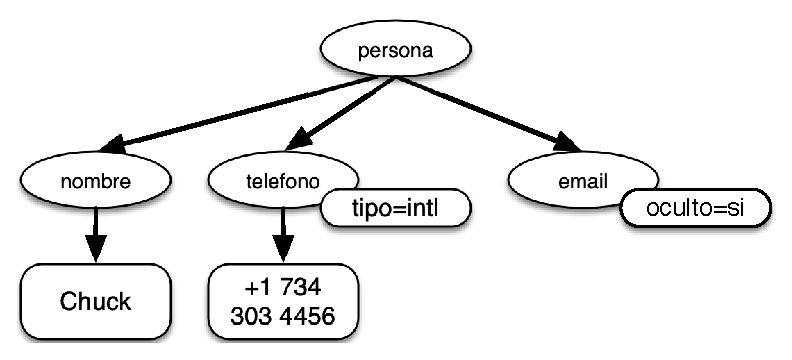
\includegraphics[keepaspectratio,alt={A Tree Representation of XML},height=2.0in]{../images/xml-tree.eps}}
\caption{A Tree Representation of XML}
\end{figure}

\section{Parsing XML}\label{parsing-xml}

\index{ElementTree} \index{ElementTree!fromstring}
\index{ElementTree!find}

Narito ang simpleng application na nagpa-parse ng ilang XML at kumukuha
ng ilang data elements mula sa XML:

\begin{Shaded}
\begin{Highlighting}[]
\ImportTok{import}\NormalTok{ xml.etree.ElementTree }\ImportTok{as}\NormalTok{ ET}

\NormalTok{data }\OperatorTok{=} \StringTok{\textquotesingle{}\textquotesingle{}\textquotesingle{}}
\StringTok{\textless{}person\textgreater{}}
\StringTok{  \textless{}name\textgreater{}Chuck\textless{}/name\textgreater{}}
\StringTok{  \textless{}phone type="intl"\textgreater{}}
\StringTok{    +1 734 303 4456}
\StringTok{  \textless{}/phone\textgreater{}}
\StringTok{  \textless{}email hide="yes" /\textgreater{}}
\StringTok{\textless{}/person\textgreater{}\textquotesingle{}\textquotesingle{}\textquotesingle{}}

\NormalTok{tree }\OperatorTok{=}\NormalTok{ ET.fromstring(data)}
\BuiltInTok{print}\NormalTok{(}\StringTok{\textquotesingle{}Name:\textquotesingle{}}\NormalTok{, tree.find(}\StringTok{\textquotesingle{}name\textquotesingle{}}\NormalTok{).text)}
\BuiltInTok{print}\NormalTok{(}\StringTok{\textquotesingle{}Attr:\textquotesingle{}}\NormalTok{, tree.find(}\StringTok{\textquotesingle{}email\textquotesingle{}}\NormalTok{).get(}\StringTok{\textquotesingle{}hide\textquotesingle{}}\NormalTok{))}

\CommentTok{\# Code: https://www.py4e.com/code3/xml1.py}
\end{Highlighting}
\end{Shaded}

Ang triple single quote
(\texttt{\textquotesingle{}\textquotesingle{}\textquotesingle{}}), pati
na rin ang triple double quote (\texttt{"""}), ay nagpapahintulot sa
paggawa ng strings na sumasaklaw sa maraming linya.

Ang pagtawag sa \texttt{fromstring} ay nagko-convert ng string
representation ng XML sa ``tree'' ng XML elements. Kapag ang XML ay nasa
tree, mayroon tayong serye ng methods na maaari nating tawagin para
kunin ang mga parte ng data mula sa XML string. Ang \texttt{find}
function ay naghahanap sa XML tree at kumukuha ng element na tumutugma
sa tinukoy na tag.

{\small
\begin{verbatim}
Name: Chuck
Attr: yes
\end{verbatim}
}

Ang paggamit ng XML parser tulad ng \texttt{ElementTree} ay may
advantage na habang ang XML sa halimbawang ito ay medyo simple,
lumalabas na mayroong maraming rules tungkol sa valid XML, at ang
paggamit ng \texttt{ElementTree} ay nagpapahintulot sa atin na kunin ang
data mula sa XML nang hindi nag-aalala tungkol sa rules ng XML syntax.

\section{Looping through nodes}\label{looping-through-nodes}

\index{ElementTree!findall} \index{ElementTree!get}

Kadalasan ang XML ay may maraming nodes at kailangan nating sumulat ng
loop para iproseso ang lahat ng nodes. Sa sumusunod na program,
naglo-loop tayo sa lahat ng \texttt{user} nodes:

\begin{Shaded}
\begin{Highlighting}[]
\ImportTok{import}\NormalTok{ xml.etree.ElementTree }\ImportTok{as}\NormalTok{ ET}

\BuiltInTok{input} \OperatorTok{=} \StringTok{\textquotesingle{}\textquotesingle{}\textquotesingle{}}
\StringTok{\textless{}stuff\textgreater{}}
\StringTok{  \textless{}users\textgreater{}}
\StringTok{    \textless{}user x="2"\textgreater{}}
\StringTok{      \textless{}id\textgreater{}001\textless{}/id\textgreater{}}
\StringTok{      \textless{}name\textgreater{}Chuck\textless{}/name\textgreater{}}
\StringTok{    \textless{}/user\textgreater{}}
\StringTok{    \textless{}user x="7"\textgreater{}}
\StringTok{      \textless{}id\textgreater{}009\textless{}/id\textgreater{}}
\StringTok{      \textless{}name\textgreater{}Brent\textless{}/name\textgreater{}}
\StringTok{    \textless{}/user\textgreater{}}
\StringTok{  \textless{}/users\textgreater{}}
\StringTok{\textless{}/stuff\textgreater{}\textquotesingle{}\textquotesingle{}\textquotesingle{}}

\NormalTok{stuff }\OperatorTok{=}\NormalTok{ ET.fromstring(}\BuiltInTok{input}\NormalTok{)}
\NormalTok{lst }\OperatorTok{=}\NormalTok{ stuff.findall(}\StringTok{\textquotesingle{}users/user\textquotesingle{}}\NormalTok{)}
\BuiltInTok{print}\NormalTok{(}\StringTok{\textquotesingle{}User count:\textquotesingle{}}\NormalTok{, }\BuiltInTok{len}\NormalTok{(lst))}

\ControlFlowTok{for}\NormalTok{ item }\KeywordTok{in}\NormalTok{ lst:}
    \BuiltInTok{print}\NormalTok{(}\StringTok{\textquotesingle{}Name\textquotesingle{}}\NormalTok{, item.find(}\StringTok{\textquotesingle{}name\textquotesingle{}}\NormalTok{).text)}
    \BuiltInTok{print}\NormalTok{(}\StringTok{\textquotesingle{}Id\textquotesingle{}}\NormalTok{, item.find(}\StringTok{\textquotesingle{}id\textquotesingle{}}\NormalTok{).text)}
    \BuiltInTok{print}\NormalTok{(}\StringTok{\textquotesingle{}Attribute\textquotesingle{}}\NormalTok{, item.get(}\StringTok{\textquotesingle{}x\textquotesingle{}}\NormalTok{))}

\CommentTok{\# Code: https://www.py4e.com/code3/xml2.py}
\end{Highlighting}
\end{Shaded}

Ang \texttt{findall} method ay kumukuha ng Python list ng subtrees na
kumakatawan sa \texttt{user} structures sa XML tree. Pagkatapos maaari
tayong sumulat ng \texttt{for} loop na tumitingin sa bawat user node, at
nagpi-print ng \texttt{name} at \texttt{id} text elements pati na rin
ang \texttt{x} attribute mula sa \texttt{user} node.

{\small
\begin{verbatim}
User count: 2
Name Chuck
Id 001
Attribute 2
Name Brent
Id 009
Attribute 7
\end{verbatim}
}

Mahalagang isama ang lahat ng parent level elements sa \texttt{findall}
statement maliban sa top level element (hal., \texttt{users/user}). Kung
hindi, ang Python ay hindi makakahanap ng anumang gustong nodes.

\begin{Shaded}
\begin{Highlighting}[]
\ImportTok{import}\NormalTok{ xml.etree.ElementTree }\ImportTok{as}\NormalTok{ ET}

\BuiltInTok{input} \OperatorTok{=} \StringTok{\textquotesingle{}\textquotesingle{}\textquotesingle{}}
\StringTok{\textless{}stuff\textgreater{}}
\StringTok{  \textless{}users\textgreater{}}
\StringTok{    \textless{}user x="2"\textgreater{}}
\StringTok{      \textless{}id\textgreater{}001\textless{}/id\textgreater{}}
\StringTok{      \textless{}name\textgreater{}Chuck\textless{}/name\textgreater{}}
\StringTok{    \textless{}/user\textgreater{}}
\StringTok{    \textless{}user x="7"\textgreater{}}
\StringTok{      \textless{}id\textgreater{}009\textless{}/id\textgreater{}}
\StringTok{      \textless{}name\textgreater{}Brent\textless{}/name\textgreater{}}
\StringTok{    \textless{}/user\textgreater{}}
\StringTok{  \textless{}/users\textgreater{}}
\StringTok{\textless{}/stuff\textgreater{}\textquotesingle{}\textquotesingle{}\textquotesingle{}}

\NormalTok{stuff }\OperatorTok{=}\NormalTok{ ET.fromstring(}\BuiltInTok{input}\NormalTok{)}

\NormalTok{lst }\OperatorTok{=}\NormalTok{ stuff.findall(}\StringTok{\textquotesingle{}users/user\textquotesingle{}}\NormalTok{)}
\BuiltInTok{print}\NormalTok{(}\StringTok{\textquotesingle{}User count:\textquotesingle{}}\NormalTok{, }\BuiltInTok{len}\NormalTok{(lst))}

\NormalTok{lst2 }\OperatorTok{=}\NormalTok{ stuff.findall(}\StringTok{\textquotesingle{}user\textquotesingle{}}\NormalTok{)}
\BuiltInTok{print}\NormalTok{(}\StringTok{\textquotesingle{}User count:\textquotesingle{}}\NormalTok{, }\BuiltInTok{len}\NormalTok{(lst2))}
\end{Highlighting}
\end{Shaded}

Ang \texttt{lst} ay nag-i-store ng lahat ng \texttt{user} elements na
nested sa loob ng kanilang \texttt{users} parent. Ang \texttt{lst2} ay
naghahanap ng \texttt{user} elements na hindi nested sa loob ng top
level \texttt{stuff} element kung saan walang anuman.

{\small
\begin{verbatim}
User count: 2
User count: 0
\end{verbatim}
}

\section{JavaScript Object Notation -
JSON}\label{javascript-object-notation---json}

\index{JSON} \index{JavaScript Object Notation}

Ang JSON format ay naging inspirasyon mula sa object at array format na
ginagamit sa JavaScript language. Pero dahil ang Python ay naimbento
bago ang JavaScript, ang syntax ng Python para sa dictionaries at lists
ay naimpluwensyahan ang syntax ng JSON. Kaya ang format ng JSON ay halos
kapareho ng kombinasyon ng Python lists at dictionaries.

Narito ang JSON encoding na halos katumbas ng simpleng XML mula sa
itaas:

\begin{Shaded}
\begin{Highlighting}[]
\FunctionTok{\{}
  \DataTypeTok{"name"} \FunctionTok{:} \StringTok{"Chuck"}\FunctionTok{,}
  \DataTypeTok{"phone"} \FunctionTok{:} \FunctionTok{\{}
    \DataTypeTok{"type"} \FunctionTok{:} \StringTok{"intl"}\FunctionTok{,}
    \DataTypeTok{"number"} \FunctionTok{:} \StringTok{"+1 734 303 4456"}
   \FunctionTok{\},}
   \DataTypeTok{"email"} \FunctionTok{:} \FunctionTok{\{}
     \DataTypeTok{"hide"} \FunctionTok{:} \StringTok{"yes"}
   \FunctionTok{\}}
\FunctionTok{\}}
\end{Highlighting}
\end{Shaded}

Mapapansin mo ang ilang pagkakaiba. Una, sa XML, maaari tayong magdagdag
ng attributes tulad ng ``intl'' sa ``phone'' tag. Sa JSON, mayroon lang
tayong key-value pairs. Gayundin ang XML ``person'' tag ay nawala,
pinalitan ng set ng outer curly braces.

Sa pangkalahatan, ang JSON structures ay mas simple kaysa sa XML dahil
ang JSON ay may mas kaunting capabilities kaysa sa XML. Pero ang JSON ay
may advantage na nagma-map ito \emph{directly} sa ilang kombinasyon ng
dictionaries at lists. At dahil halos lahat ng programming languages ay
may katumbas sa dictionaries at lists ng Python, ang JSON ay napakalikas
na format para magkaroon ng dalawang cooperating programs na magpalitan
ng data.

Ang JSON ay mabilis na naging format ng pagpipilian para sa halos lahat
ng data exchange sa pagitan ng applications dahil sa relatibong
simplicity nito kumpara sa XML.

\section{Parsing JSON}\label{parsing-json}

Ginagawa natin ang JSON natin sa pamamagitan ng pag-nest ng dictionaries
at lists ayon sa pangangailangan. Sa halimbawang ito, kinakatawan natin
ang list ng users kung saan ang bawat user ay set ng key-value pairs
(i.e., dictionary). Kaya mayroon tayong list ng dictionaries.

Sa sumusunod na program, ginagamit natin ang built-in \texttt{json}
library para mag-parse ng JSON at magbasa sa data. I-compare ito nang
mabuti sa katumbas na XML data at code sa itaas. Ang JSON ay may mas
kaunting detalye, kaya dapat nating malaman nang maaga na nakakakuha
tayo ng list at ang list ay ng users at ang bawat user ay set ng
key-value pairs. Ang JSON ay mas succinct (advantage) pero mas kaunti
rin ang self-describing (a disadvantage).

\begin{Shaded}
\begin{Highlighting}[]
\ImportTok{import}\NormalTok{ json}

\NormalTok{data }\OperatorTok{=} \StringTok{\textquotesingle{}\textquotesingle{}\textquotesingle{}}
\StringTok{[}
\StringTok{  \{ "id" : "001",}
\StringTok{    "x" : "2",}
\StringTok{    "name" : "Chuck"}
\StringTok{  \} ,}
\StringTok{  \{ "id" : "009",}
\StringTok{    "x" : "7",}
\StringTok{    "name" : "Brent"}
\StringTok{  \}}
\StringTok{]\textquotesingle{}\textquotesingle{}\textquotesingle{}}

\NormalTok{info }\OperatorTok{=}\NormalTok{ json.loads(data)}
\BuiltInTok{print}\NormalTok{(}\StringTok{\textquotesingle{}User count:\textquotesingle{}}\NormalTok{, }\BuiltInTok{len}\NormalTok{(info))}

\ControlFlowTok{for}\NormalTok{ item }\KeywordTok{in}\NormalTok{ info:}
    \BuiltInTok{print}\NormalTok{(}\StringTok{\textquotesingle{}Name\textquotesingle{}}\NormalTok{, item[}\StringTok{\textquotesingle{}name\textquotesingle{}}\NormalTok{])}
    \BuiltInTok{print}\NormalTok{(}\StringTok{\textquotesingle{}Id\textquotesingle{}}\NormalTok{, item[}\StringTok{\textquotesingle{}id\textquotesingle{}}\NormalTok{])}
    \BuiltInTok{print}\NormalTok{(}\StringTok{\textquotesingle{}Attribute\textquotesingle{}}\NormalTok{, item[}\StringTok{\textquotesingle{}x\textquotesingle{}}\NormalTok{])}

\CommentTok{\# Code: https://www.py4e.com/code3/json2.py}
\end{Highlighting}
\end{Shaded}

Kung i-compare mo ang code para kunin ang data mula sa parsed JSON at
XML makikita mo na ang nakukuha natin mula sa \texttt{json.loads()} ay
Python list na dinadaanan natin gamit ang \texttt{for} loop, at ang
bawat item sa loob ng list na iyon ay Python dictionary. Kapag na-parse
na ang JSON, maaari nating gamitin ang Python index operator para kunin
ang iba't ibang bits ng data para sa bawat user. Hindi natin kailangang
gamitin ang JSON library para mag-dig sa parsed JSON, dahil ang returned
data ay simpleng native Python structures.

Ang output ng program na ito ay eksaktong pareho sa XML version sa
itaas.

{\small
\begin{verbatim}
User count: 2
Name Chuck
Id 001
Attribute 2
Name Brent
Id 009
Attribute 7
\end{verbatim}
}

Sa pangkalahatan, mayroong industry trend palayo sa XML at patungo sa
JSON para sa web services. Dahil ang JSON ay mas simple at mas direktang
nagma-map sa native data structures na mayroon na tayo sa programming
languages, ang parsing at data extraction code ay karaniwang mas simple
at mas direkta kapag gumagamit ng JSON. Pero ang XML ay mas
self-descriptive kaysa sa JSON at kaya mayroong ilang applications kung
saan ang XML ay nananatiling may advantage. Halimbawa, karamihan ng word
processors ay nag-i-store ng documents internally gamit ang XML sa halip
na JSON.

\section{Application Programming
Interfaces}\label{application-programming-interfaces}

Mayroon na tayong kakayahang magpalitan ng data sa pagitan ng
applications gamit ang Hypertext Transport Protocol (HTTP) at paraan
para kumatawan sa complex data na ipinapadala natin pabalik-balik sa
pagitan ng mga applications na ito gamit ang eXtensible Markup Language
(XML) o JavaScript Object Notation (JSON).

Ang susunod na hakbang ay simulan na tukuyin at dokumentado ang
``contracts'' sa pagitan ng applications gamit ang mga techniques na
ito. Ang pangkalahatang pangalan para sa mga application-to-application
contracts na ito ay \emph{Application Program Interfaces} (APIs). Kapag
gumagamit tayo ng API, karaniwang isang program ang gumagawa ng set ng
\emph{services} na available para gamitin ng iba pang applications at
nagpu-publish ng APIs (i.e., ang ``rules'') na dapat sundin para
ma-access ang services na ibinigay ng program.

Kapag nagsisimula na tayong gumawa ng programs natin kung saan ang
functionality ng aming program ay kasama ang access sa services na
ibinigay ng iba pang programs, tinatawag natin ang approach na
\emph{Service-oriented architecture} (SOA). Ang SOA approach ay isa kung
saan ang overall application natin ay gumagamit ng services ng iba pang
applications. Ang non-SOA approach ay kung saan ang application ay isang
solong standalone application na naglalaman ng lahat ng code na
kailangan para i-implement ang application.

Nakikita natin ang maraming halimbawa ng SOA kapag gumagamit tayo ng
web. Maaari tayong pumunta sa isang web site at mag-book ng air travel,
hotels, at automobiles lahat mula sa isang site. Ang data para sa hotels
ay hindi naka-store sa airline computers. Sa halip, ang airline
computers ay nakikipag-ugnayan sa services sa hotel computers at
kumukuha ng hotel data at ipinakita ito sa user. Kapag sumang-ayon ang
user na gumawa ng hotel reservation gamit ang airline site, ang airline
site ay gumagamit ng iba pang web service sa hotel systems para talagang
gawin ang reservation. At kapag oras na para singilin ang credit card mo
para sa buong transaction, iba pang computers pa rin ang kasangkot sa
proseso.

\begin{figure}
\centering
\pandocbounded{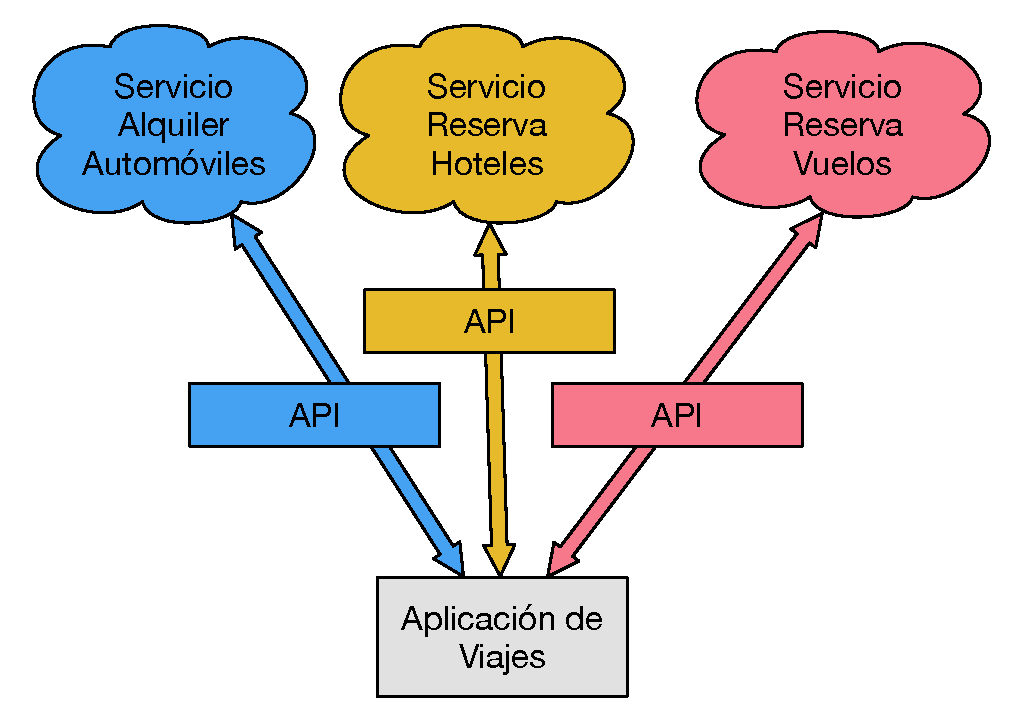
\includegraphics[keepaspectratio,alt={Service-oriented architecture},height=3.0in]{../images/soa.eps}}
\caption{Service-oriented architecture}
\end{figure}

Ang Service-oriented architecture ay may maraming advantages, kasama
ang: (1) palaging nagma-maintain lang tayo ng isang kopya ng data (ito
ay partikular na mahalaga para sa mga bagay tulad ng hotel reservations
kung saan ayaw nating mag-over-commit) at (2) ang mga may-ari ng data ay
maaaring magtakda ng rules tungkol sa paggamit ng kanilang data. Sa mga
advantages na ito, ang SOA system ay dapat maingat na idinisenyo para
magkaroon ng magandang performance at matugunan ang pangangailangan ng
user.

Kapag ang application ay gumagawa ng set ng services sa API nito na
available sa web, tinatawag natin ang mga ito na \emph{web services}.

\section{Security and API usage}\label{security-and-api-usage}

\index{OAuth} \index{API!key}

Napakakaraniwan na kailangan mo ng API key para magamit ang API ng
vendor. Ang pangkalahatang ideya ay gusto nilang malaman kung sino ang
gumagamit ng services nila at kung gaano karami ang ginagamit ng bawat
user. Marahil mayroon silang libre at bayad na tiers ng services nila o
may policy na naglilimita sa bilang ng requests na maaaring gawin ng
isang indibidwal sa partikular na panahon period.

Minsan kapag nakuha mo na ang API key mo, simpleng isama mo lang ang key
bilang parte ng POST data o marahil bilang parameter sa URL kapag
tinatawag ang API.

Sa ibang pagkakataon, ang vendor ay gusto ng mas mataas na assurance ng
source ng requests at kaya inaasahan nila na magpadala ka ng
cryptographically signed messages gamit ang shared keys at secrets. Ang
napakakaraniwang teknolohiya na ginagamit para mag-sign ng requests sa
Internet ay tinatawag na \emph{OAuth}. Maaari kang magbasa pa tungkol sa
OAuth protocol sa \href{http://www.oauth.net}{www.oauth.net}.

Sa kabutihang palad mayroong ilang maginhawa at libreng OAuth libraries
para maiwasan mong sumulat ng OAuth implementation mula sa simula sa
pamamagitan ng pagbabasa ng specification. Ang mga libraries na ito ay
may iba't ibang complexity at may iba't ibang antas ng richness. Ang
OAuth web site ay may impormasyon tungkol sa iba't ibang OAuth
libraries.

\section{Glossary}\label{glossary-12}

\begin{description}
\tightlist
\item[API]
Application Program Interface - Contract sa pagitan ng applications na
nagde-define ng patterns ng interaction sa pagitan ng dalawang
application components. \index{API}
\item[ElementTree]
Built-in Python library na ginagamit para mag-parse ng XML data.
\index{ElementTree}
\item[JSON]
JavaScript Object Notation - Format na nagpapahintulot sa markup ng
structured data batay sa syntax ng JavaScript Objects. \index{JSON}
\index{JavaScript Object Notation}
\item[SOA]
Service-Oriented Architecture - Kapag ang application ay gawa sa
components na konektado sa network. \index{SOA}
\index{Service Oriented Architecture}
\item[XML]
eXtensible Markup Language - Format na nagpapahintulot sa markup ng
structured data. \index{XML} \index{eXtensible Markup Language}
\end{description}

\chapter{Object-oriented programming}\label{object-oriented-programming}

\section{Managing larger programs}\label{managing-larger-programs}

\index{object-oriented}

Sa simula ng libro na ito, nakabuo tayo ng apat na basic programming
patterns na ginagamit natin para gumawa ng programs:

\begin{itemize}
\tightlist
\item
  Sequential code
\item
  Conditional code (if statements)
\item
  Repetitive code (loops)
\item
  Store and reuse (functions)
\end{itemize}

Sa mga susunod na chapters, nag-explore tayo ng simple variables pati na
rin ng collection data structures tulad ng lists, tuples, at
dictionaries.

Habang gumagawa tayo ng programs, nagde-design tayo ng data structures
at sumusulat ng code para manipulahin ang mga data structures na iyon.
Mayroong maraming paraan para sumulat ng programs at sa ngayon, malamang
nakasulat ka na ng ilang programs na ``hindi masyadong elegant'' at iba
pang programs na ``mas elegant''. Kahit na ang programs mo ay maaaring
maliit, nagsisimula ka nang makita kung paano mayroong kaunting sining
at aesthetic sa pagsusulat ng code.

Habang ang programs ay nagiging milyun-milyong linya ang haba, nagiging
mas mahalaga na sumulat ng code na madaling maintindihan. Kung
nagtatrabaho ka sa million-line program, hindi mo kailanman maaaring
panatilihin ang buong program sa isip mo nang sabay. Kailangan natin ng
mga paraan para hatiin ang malalaking programs sa maraming mas maliliit
na piraso para mas kaunti ang dapat tingnan kapag nagso-solve ng
problema, nagfi-fix ng bug, o nagdaragdag ng bagong feature.

Sa isang paraan, ang object oriented programming ay paraan para ayusin
ang code mo para maaari mong i-zoom ang 50 lines ng code at maintindihan
ito habang hindi pinapansin ang iba pang 999,950 lines ng code sa
sandaling iyon.

\section{Getting started}\label{getting-started}

Tulad ng maraming aspeto ng programming, kailangan na matutunan ang mga
konsepto ng object oriented programming bago mo magamit ang mga ito nang
epektibo. Dapat mong lapitan ang chapter na ito bilang paraan para
matuto ng ilang terms at concepts at magtrabaho sa ilang simpleng
halimbawa para maglagay ng pundasyon para sa pag-aaral sa hinaharap.

Ang pangunahing resulta ng chapter na ito ay magkaroon ng basic na
pag-unawa kung paano ginagawa ang objects at kung paano sila gumagana at
pinakamahalaga kung paano ginagamit natin ang capabilities ng objects na
ibinigay sa atin ng Python at Python libraries.

\section{Using objects}\label{using-objects}

Tulad ng lumalabas, gumagamit na tayo ng objects sa buong libro na ito.
Ang Python ay nagbibigay sa atin ng maraming built-in objects. Narito
ang ilang simpleng code kung saan ang unang ilang linya ay dapat
pakiramdam na napakasimple at natural sa iyo.

\index{list object}

\begin{Shaded}
\begin{Highlighting}[]
\NormalTok{stuff }\OperatorTok{=} \BuiltInTok{list}\NormalTok{()}
\NormalTok{stuff.append(}\StringTok{\textquotesingle{}python\textquotesingle{}}\NormalTok{)}
\NormalTok{stuff.append(}\StringTok{\textquotesingle{}chuck\textquotesingle{}}\NormalTok{)}
\NormalTok{stuff.sort()}
\BuiltInTok{print}\NormalTok{ (stuff[}\DecValTok{0}\NormalTok{])}
\BuiltInTok{print}\NormalTok{ (stuff.}\FunctionTok{\_\_getitem\_\_}\NormalTok{(}\DecValTok{0}\NormalTok{))}
\BuiltInTok{print}\NormalTok{ (}\BuiltInTok{list}\NormalTok{.}\FunctionTok{\_\_getitem\_\_}\NormalTok{(stuff,}\DecValTok{0}\NormalTok{))}

\CommentTok{\# Code: https://www.py4e.com/code3/objects.py}
\end{Highlighting}
\end{Shaded}

Sa halip na tumuon sa kung ano ang nagagawa ng mga linyang ito, tingnan
natin kung ano ang talagang nangyayari mula sa punto de vista ng
object-oriented programming. Huwag mag-alala kung ang sumusunod na
paragraphs ay hindi makakasensya sa unang pagkakataon na binabasa mo
sila dahil hindi pa natin tinukoy ang lahat ng terms na ito.

Ang unang linya ay \emph{gumagawa} ng object ng type na \texttt{list},
ang pangalawa at pangatlong linya ay \emph{tumatawag} sa
\texttt{append()} \emph{method}, ang ikaapat na linya ay tumatawag sa
\texttt{sort()} method, at ang ikalimang linya ay \emph{kumukuha} ng
item sa posisyon 0.

Ang ikaanim na linya ay tumatawag sa \texttt{\_\_getitem\_\_()} method
sa \texttt{stuff} list na may parameter na zero.

\begin{Shaded}
\begin{Highlighting}[]
\BuiltInTok{print}\NormalTok{ (stuff.}\FunctionTok{\_\_getitem\_\_}\NormalTok{(}\DecValTok{0}\NormalTok{))}
\end{Highlighting}
\end{Shaded}

Ang ikapitong linya ay mas verbose na paraan ng pagkuha ng 0th item sa
list.

\begin{Shaded}
\begin{Highlighting}[]
\BuiltInTok{print}\NormalTok{ (}\BuiltInTok{list}\NormalTok{.}\FunctionTok{\_\_getitem\_\_}\NormalTok{(stuff,}\DecValTok{0}\NormalTok{))}
\end{Highlighting}
\end{Shaded}

Sa code na ito, tumatawag tayo sa \texttt{\_\_getitem\_\_} method sa
\texttt{list} class at \emph{nagpapasa} ng list at item na gusto nating
kunin mula sa list bilang parameters.

Ang huling tatlong linya ng program ay katumbas, pero mas maginhawa na
simpleng gamitin ang square bracket syntax para maghanap ng item sa
partikular na posisyon sa list.

Maaari tayong tumingin sa capabilities ng object sa pamamagitan ng
pagtingin sa output ng \texttt{dir()} function:

{\small
\begin{verbatim}
>>> stuff = list()
>>> dir(stuff)
['__add__', '__class__', '__contains__', '__delattr__',
'__delitem__', '__dir__', '__doc__', '__eq__',
'__format__', '__ge__', '__getattribute__', '__getitem__',
'__gt__', '__hash__', '__iadd__', '__imul__', '__init__',
'__iter__', '__le__', '__len__', '__lt__', '__mul__',
'__ne__', '__new__', '__reduce__', '__reduce_ex__',
'__repr__', '__reversed__', '__rmul__', '__setattr__',
'__setitem__', '__sizeof__', '__str__', '__subclasshook__',
'append', 'clear', 'copy', 'count', 'extend', 'index',
'insert', 'pop', 'remove', 'reverse', 'sort']
>>>
\end{verbatim}
}

Ang natitirang parte ng chapter na ito ay tutukuyin ang lahat ng terms
sa itaas kaya siguraduhing bumalik pagkatapos mong tapusin ang chapter
at basahin ulit ang paragraphs sa itaas para suriin ang iyong pag-unawa.

\section{Starting with programs}\label{starting-with-programs}

Ang program sa pinakabasic na form nito ay tumatanggap ng ilang input,
gumagawa ng ilang processing, at gumagawa ng ilang output. Ang elevator
conversion program natin ay nagpapakita ng napakaikli pero kumpletong
program na nagpapakita ng lahat ng tatlong hakbang na ito.

\begin{Shaded}
\begin{Highlighting}[]
\NormalTok{usf }\OperatorTok{=} \BuiltInTok{input}\NormalTok{(}\StringTok{\textquotesingle{}Enter the US Floor Number: \textquotesingle{}}\NormalTok{)}
\NormalTok{wf }\OperatorTok{=} \BuiltInTok{int}\NormalTok{(usf) }\OperatorTok{{-}} \DecValTok{1}
\BuiltInTok{print}\NormalTok{(}\StringTok{\textquotesingle{}Non{-}US Floor Number is\textquotesingle{}}\NormalTok{,wf)}

\CommentTok{\# Code: https://www.py4e.com/code3/elev.py}
\end{Highlighting}
\end{Shaded}

Kung mag-iisip tayo nang kaunti tungkol sa program na ito, mayroong
``outside world'' at ang program. Ang input at output aspects ay kung
saan nakikipag-ugnayan ang program sa outside world. Sa loob ng program
mayroon tayong code at data para makamit ang gawain na idinisenyo ng
program na solusyonan.

\begin{figure}
\centering
\pandocbounded{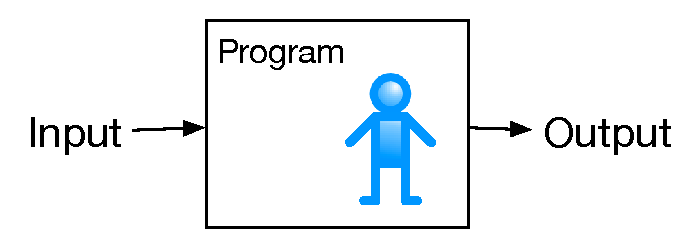
\includegraphics[keepaspectratio,alt={A Program},height=1.20in]{../images/program.eps}}
\caption{A Program}
\end{figure}

Ang isang paraan para isipin ang object-oriented programming ay
hinihiwalay nito ang program natin sa maraming ``zones.'' Ang bawat zone
ay naglalaman ng ilang code at data (tulad ng program) at may well
defined interactions sa outside world at iba pang zones sa loob ng
program.

Kung titingnan natin ang link extraction application kung saan ginamit
natin ang BeautifulSoup library, makikita natin ang program na ginawa sa
pamamagitan ng pagkokonekta ng iba't ibang objects nang magkasama para
makamit ang gawain:

\index{BeautifulSoup} \index{HTML} \index{parsing!HTML}

\begin{Shaded}
\begin{Highlighting}[]
\CommentTok{\# To run this, download the BeautifulSoup zip file}
\CommentTok{\# http://www.py4e.com/code3/bs4.zip}
\CommentTok{\# or pip install beautifulsoup4 to ensure you have the latest version}
\CommentTok{\# and unzip it in the same directory as this file}

\ImportTok{import}\NormalTok{ urllib.request, urllib.parse, urllib.error}
\ImportTok{from}\NormalTok{ bs4 }\ImportTok{import}\NormalTok{ BeautifulSoup}
\ImportTok{import}\NormalTok{ ssl }\CommentTok{\# defauts to certicate verification and most secure protocol (now TLS)}

\CommentTok{\# Ignore SSL/TLS certificate errors}
\NormalTok{ctx }\OperatorTok{=}\NormalTok{ ssl.create\_default\_context()}
\NormalTok{ctx.check\_hostname }\OperatorTok{=} \VariableTok{False}
\NormalTok{ctx.verify\_mode }\OperatorTok{=}\NormalTok{ ssl.CERT\_NONE}

\NormalTok{url }\OperatorTok{=} \BuiltInTok{input}\NormalTok{(}\StringTok{\textquotesingle{}Enter {-} \textquotesingle{}}\NormalTok{)}
\NormalTok{html }\OperatorTok{=}\NormalTok{ urllib.request.urlopen(url, context}\OperatorTok{=}\NormalTok{ctx).read()}
\NormalTok{soup }\OperatorTok{=}\NormalTok{ BeautifulSoup(html, }\StringTok{\textquotesingle{}html.parser\textquotesingle{}}\NormalTok{)}

\CommentTok{\# Retrieve all of the anchor tags}
\NormalTok{tags }\OperatorTok{=}\NormalTok{ soup(}\StringTok{\textquotesingle{}a\textquotesingle{}}\NormalTok{)}
\ControlFlowTok{for}\NormalTok{ tag }\KeywordTok{in}\NormalTok{ tags:}
    \BuiltInTok{print}\NormalTok{(tag.get(}\StringTok{\textquotesingle{}href\textquotesingle{}}\NormalTok{, }\VariableTok{None}\NormalTok{))}

\CommentTok{\# Code: https://www.py4e.com/code3/urllinks.py}
\end{Highlighting}
\end{Shaded}

Binabasa natin ang URL sa string at pagkatapos ipinapasa iyon sa
\texttt{urllib} para kunin ang data mula sa web. Ang \texttt{urllib}
library ay gumagamit ng \texttt{socket} library para gumawa ng aktwal na
network connection para kunin ang data. Kinukuha natin ang string na
ibinabalik ng \texttt{urllib} at ibinibigay sa BeautifulSoup para
i-parse. Ang BeautifulSoup ay gumagamit ng object na
\texttt{html.parser}\footnote{https://docs.python.org/3/library/html.parser.html}
at nagre-return ng object. Tumatawag tayo sa \texttt{tags()} method sa
returned object na nagre-return ng dictionary ng tag objects. Naglo-loop
tayo sa tags at tumatawag sa \texttt{get()} method para sa bawat tag
para mag-print ng \texttt{href} attribute.

Maaari tayong gumuhit ng larawan ng program na ito at kung paano
gumagana nang magkasama ang objects.

\begin{figure}
\centering
\pandocbounded{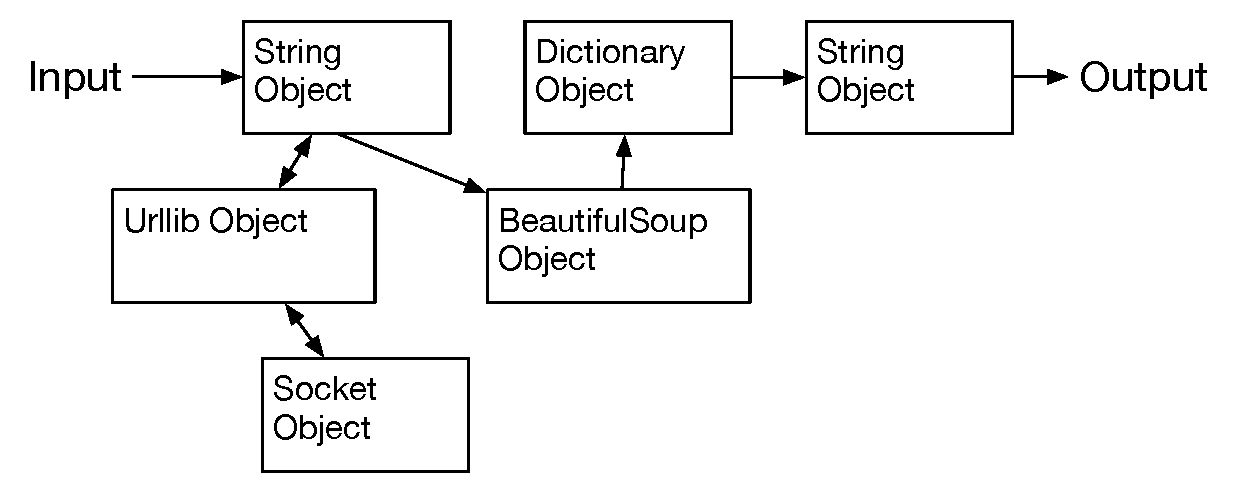
\includegraphics[keepaspectratio,alt={A Program as Network of Objects},height=1.50in]{../images/program-oo.eps}}
\caption{A Program as Network of Objects}
\end{figure}

Ang susi dito ay hindi maintindihan nang perpekto kung paano gumagana
ang program na ito pero makita kung paano gumagawa tayo ng network ng
interacting objects at nag-o-orchestrate ng paggalaw ng impormasyon sa
pagitan ng objects para gumawa ng program. Mahalaga rin na tandaan na
kapag tiningnan mo ang program na iyon ilang chapters pabalik, maaari
mong ganap na maintindihan kung ano ang nangyayari sa program nang hindi
man lang napagtanto na ang program ay ``nag-o-orchestrate ng paggalaw ng
data sa pagitan ng objects.'' Ito ay simpleng mga linya ng code na
gumagawa ng trabaho.

\section{Subdividing a problem}\label{subdividing-a-problem}

Isa sa mga advantages ng object-oriented approach ay maaari nitong itago
ang complexity. Halimbawa, habang kailangan nating malaman kung paano
gamitin ang \texttt{urllib} at BeautifulSoup code, hindi natin
kailangang malaman kung paano gumagana ang mga libraries na iyon
internally. Nagpapahintulot ito sa atin na tumuon sa parte ng problema
na kailangan nating solusyonan at huwag pansinin ang iba pang parte ng
program.

\begin{figure}
\centering
\pandocbounded{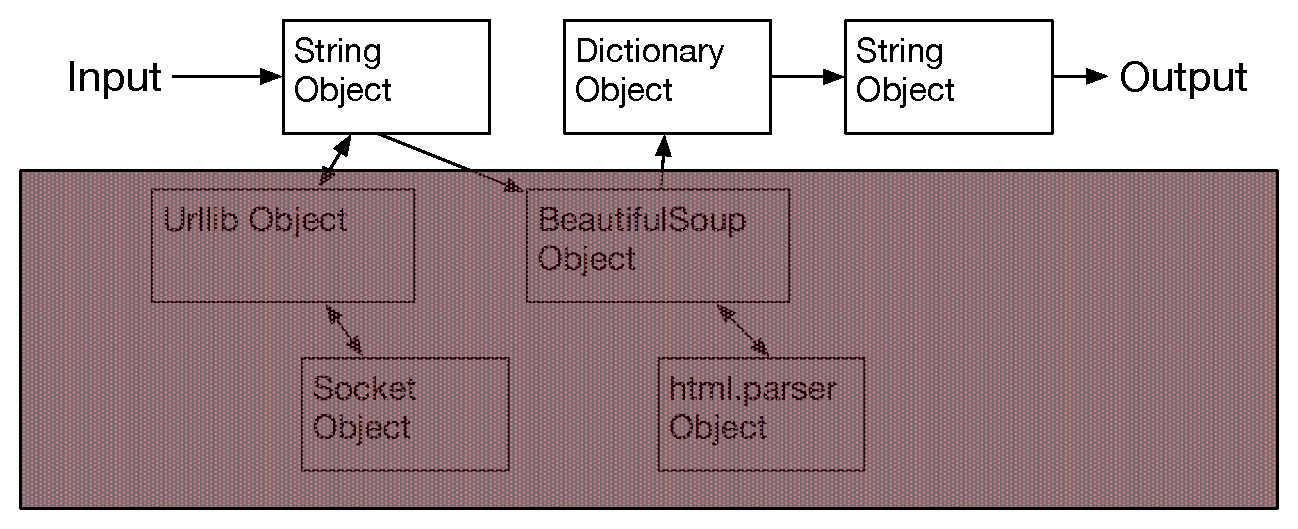
\includegraphics[keepaspectratio,alt={Ignoring Detail When Using an Object},height=1.50in]{../images/program-oo-code.eps}}
\caption{Ignoring Detail When Using an Object}
\end{figure}

Ang kakayahang ito na tumuon eksklusibo sa parte ng program na
pinapahalagahan natin at huwag pansinin ang natitira ay
kapaki-pakinabang din sa mga developers ng objects na ginagamit natin.
Halimbawa, ang mga programmers na gumagawa ng BeautifulSoup ay hindi
kailangang malaman o mag-alala tungkol sa kung paano natin kinukuha ang
HTML page natin, kung ano ang mga parte na gusto nating basahin, o kung
ano ang plano nating gawin sa data na kinukuha natin mula sa web page.

\begin{figure}
\centering
\pandocbounded{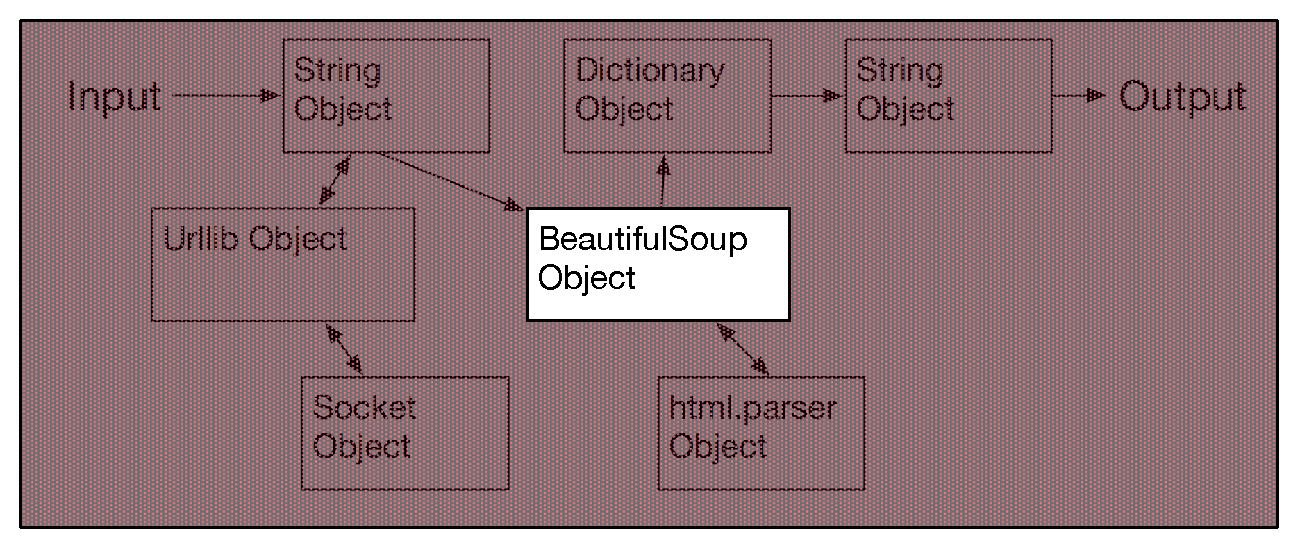
\includegraphics[keepaspectratio,alt={Ignoring Detail When Building an Object},height=1.50in]{../images/program-oo-bs4.eps}}
\caption{Ignoring Detail When Building an Object}
\end{figure}

\section{Our first Python object}\label{our-first-python-object}

Sa basic level, ang object ay simpleng ilang code kasama ang data
structures na mas maliit kaysa sa buong program. Ang pagtukoy ng
function ay nagpapahintulot sa atin na mag-store ng kaunting code at
bigyan ito ng pangalan at pagkatapos tawagin ang code na iyon gamit ang
pangalan ng function.

Ang object ay maaaring maglalaman ng ilang functions (na tinatawag
nating \emph{methods}) pati na rin ng data na ginagamit ng mga functions
na iyon. Tinatawag natin ang data items na parte ng object na
\emph{attributes}.

\index{class keyword}

Ginagamit natin ang \texttt{class} keyword para tukuyin ang data at code
na gagawin ng bawat isa sa objects. Ang class keyword ay kasama ang
pangalan ng class at nagsisimula ng indented block ng code kung saan
isinasama natin ang attributes (data) at methods (code).

\begin{Shaded}
\begin{Highlighting}[]
\KeywordTok{class}\NormalTok{ PartyAnimal:}

   \KeywordTok{def} \FunctionTok{\_\_init\_\_}\NormalTok{(}\VariableTok{self}\NormalTok{):}
     \VariableTok{self}\NormalTok{.x }\OperatorTok{=} \DecValTok{0}

   \KeywordTok{def}\NormalTok{ party(}\VariableTok{self}\NormalTok{) :}
     \VariableTok{self}\NormalTok{.x }\OperatorTok{=} \VariableTok{self}\NormalTok{.x }\OperatorTok{+} \DecValTok{1}
     \BuiltInTok{print}\NormalTok{(}\StringTok{"So far"}\NormalTok{,}\VariableTok{self}\NormalTok{.x)}

\NormalTok{an }\OperatorTok{=}\NormalTok{ PartyAnimal()}
\NormalTok{an.party()}
\NormalTok{an.party()}
\NormalTok{an.party()}

\CommentTok{\# Code: https://www.py4e.com/code3/party2.py}
\end{Highlighting}
\end{Shaded}

Ang bawat method ay mukhang function, nagsisimula sa \texttt{def}
keyword at binubuo ng indented block ng code.

Ang unang method ay specially-named method na tinatawag na
\texttt{\_\_init\_\_()}. Ang method na ito ay tinatawag para gumawa ng
anumang initial setup ng data na gusto nating i-store sa object. Sa
class na ito nag-a-allocate tayo ng \texttt{x} attribute gamit ang dot
notation at ini-initialize ito sa zero.

\begin{Shaded}
\begin{Highlighting}[]
    \VariableTok{self}\NormalTok{.x }\OperatorTok{=} \DecValTok{0}
\end{Highlighting}
\end{Shaded}

Ang iba pang method na pinangalanang \texttt{party}. Ang lahat ng
methods ay may espesyal na unang parameter na pinangalanan natin ayon sa
convention na \texttt{self}. Ang unang parameter ay nagbibigay sa atin
ng access sa object instance para maaari tayong mag-set ng attributes at
tumawag ng methods gamit ang dot notation.

Tulad ng \texttt{def} keyword ay hindi nagdudulot na ma-execute ang
function code, ang \texttt{class} keyword ay hindi gumagawa ng object.
Sa halip, ang \texttt{class} keyword ay nagde-define ng template na
nagpapahiwatig kung ano ang data at code na maglalaman sa bawat object
ng type na \texttt{PartyAnimal}. Ang class ay parang cookie cutter at
ang objects na ginawa gamit ang class ay ang cookies\footnote{Cookie
  image copyright CC-BY
  https://www.flickr.com/photos/dinnerseries/23570475099}. Hindi mo
nilalagay ang frosting sa cookie cutter; nilalagay mo ang frosting sa
cookies, at maaari kang maglagay ng iba't ibang frosting sa bawat
cookie.

\begin{figure}
\centering
\pandocbounded{\includegraphics[keepaspectratio,alt={A Class and Two Objects},height=2.0in]{../photos/cookie_cutter_flickr_Didriks.eps}}
\caption{A Class and Two Objects}
\end{figure}

Kung magpapatuloy tayo sa sample program na ito, makikita natin ang
unang executable line ng code:

\begin{Shaded}
\begin{Highlighting}[]
\NormalTok{an }\OperatorTok{=}\NormalTok{ PartyAnimal()}
\end{Highlighting}
\end{Shaded}

\index{construct} \index{object} \index{instance} \index{class}

Dito natin ini-instruct ang Python na gumawa (i.e., create) ng
\emph{object} o \emph{instance} ng class na \texttt{PartyAnimal}. Mukha
itong function call sa class mismo. Ang Python ay gumagawa ng object na
may tamang data at methods at nagre-return ng object na pagkatapos ay
na-a-assign sa variable na \texttt{an}. Sa isang paraan ito ay medyo
katulad ng sumusunod na linya na ginagamit natin sa buong panahon:

\begin{Shaded}
\begin{Highlighting}[]
\NormalTok{counts }\OperatorTok{=} \BuiltInTok{dict}\NormalTok{()}
\end{Highlighting}
\end{Shaded}

Dito ini-instruct natin ang Python na gumawa ng object gamit ang
\texttt{dict} template (nandito na sa Python), ibalik ang instance ng
dictionary, at i-assign ito sa variable na \texttt{counts}.

Kapag ang \texttt{PartyAnimal} class ay ginagamit para gumawa ng object,
ang variable na \texttt{an} ay ginagamit para tumuro sa object na iyon.
Ginagamit natin ang \texttt{an} para ma-access ang code at data para sa
partikular na instance ng \texttt{PartyAnimal} class.

Ang bawat Partyanimal object/instance ay naglalaman sa loob nito ng
variable na \texttt{x} at method/function na pinangalanang
\texttt{party}. Tumatawag tayo sa \texttt{party} method sa linyang ito:

\begin{Shaded}
\begin{Highlighting}[]
\NormalTok{an.party()}
\end{Highlighting}
\end{Shaded}

Kapag ang \texttt{party} method ay tinatawag, ang unang parameter (na
tinatawag natin ayon sa convention na \texttt{self}) ay tumuturo sa
partikular na instance ng PartyAnimal object na tinatawag ang
\texttt{party}. Sa loob ng \texttt{party} method, nakikita natin ang
linya:

\begin{Shaded}
\begin{Highlighting}[]
\VariableTok{self}\NormalTok{.x }\OperatorTok{=} \VariableTok{self}\NormalTok{.x }\OperatorTok{+} \DecValTok{1}
\end{Highlighting}
\end{Shaded}

Ang syntax na ito gamit ang \emph{dot} operator ay nagsasabing `ang x sa
loob ng self.' Sa bawat pagkakataon na tinatawag ang \texttt{party()},
ang internal \texttt{x} value ay na-i-increment ng 1 at ang value ay
na-pi-print.

Ang sumusunod na linya ay isa pang paraan para tawagin ang
\texttt{party} method sa loob ng \texttt{an} object:

\begin{Shaded}
\begin{Highlighting}[]
\NormalTok{PartyAnimal.party(an)}
\end{Highlighting}
\end{Shaded}

Sa variation na ito, na-a-access natin ang code mula sa loob ng class at
tahasang ipinapasa ang object pointer na \texttt{an} bilang unang
parameter (i.e., \texttt{self} sa loob ng method). Maaari mong isipin
ang \texttt{an.party()} bilang shorthand para sa linya sa itaas.

Kapag nag-e-execute ang program, gumagawa ito ng sumusunod na output:

{\small
\begin{verbatim}
So far 1
So far 2
So far 3
So far 4
\end{verbatim}
}

Ang object ay ginawa, at ang \texttt{party} method ay tinawag nang apat
na beses, parehong nag-i-increment at nagpi-print ng value para sa
\texttt{x} sa loob ng \texttt{an} object.

\section{Classes as types}\label{classes-as-types}

\index{dir} \index{type}

Tulad ng nakita natin, sa Python lahat ng variables ay may type. Maaari
nating gamitin ang built-in \texttt{dir} function para suriin ang
capabilities ng variable. Maaari din nating gamitin ang \texttt{type} at
\texttt{dir} sa mga classes na ginagawa natin.

\begin{Shaded}
\begin{Highlighting}[]
\KeywordTok{class}\NormalTok{ PartyAnimal:}

   \KeywordTok{def} \FunctionTok{\_\_init\_\_}\NormalTok{(}\VariableTok{self}\NormalTok{):}
     \VariableTok{self}\NormalTok{.x }\OperatorTok{=} \DecValTok{0}

   \KeywordTok{def}\NormalTok{ party(}\VariableTok{self}\NormalTok{) :}
     \VariableTok{self}\NormalTok{.x }\OperatorTok{=} \VariableTok{self}\NormalTok{.x }\OperatorTok{+} \DecValTok{1}
     \BuiltInTok{print}\NormalTok{(}\StringTok{"So far"}\NormalTok{,}\VariableTok{self}\NormalTok{.x)}

\NormalTok{an }\OperatorTok{=}\NormalTok{ PartyAnimal()}
\BuiltInTok{print}\NormalTok{ (}\StringTok{"Type"}\NormalTok{, }\BuiltInTok{type}\NormalTok{(an))}
\BuiltInTok{print}\NormalTok{ (}\StringTok{"Dir "}\NormalTok{, }\BuiltInTok{dir}\NormalTok{(an))}
\BuiltInTok{print}\NormalTok{ (}\StringTok{"Type"}\NormalTok{, }\BuiltInTok{type}\NormalTok{(an.x))}
\BuiltInTok{print}\NormalTok{ (}\StringTok{"Type"}\NormalTok{, }\BuiltInTok{type}\NormalTok{(an.party))}

\CommentTok{\# Code: https://www.py4e.com/code3/party3.py}
\end{Highlighting}
\end{Shaded}

Kapag nag-e-execute ang program na ito, gumagawa ito ng sumusunod na
output:

{\small
\begin{verbatim}
Type <class '__main__.PartyAnimal'>
Dir  ['__class__', '__delattr__', ...
'__sizeof__', '__str__', '__subclasshook__',
'__weakref__', 'party', 'x']
Type <class 'int'>
Type <class 'method'>
\end{verbatim}
}

Makikita mo na gamit ang \texttt{class} keyword, gumawa tayo ng bagong
type. Mula sa \texttt{dir} output, makikita mo na parehong \texttt{x}
integer attribute at \texttt{party} method ay available sa object.

\section{Object lifecycle}\label{object-lifecycle}

\index{constructor} \index{destructor} \index{object lifecycle}

Sa naunang mga halimbawa, nagde-define tayo ng class (template),
gumagamit ng class na iyon para gumawa ng instance ng class na iyon
(object), at pagkatapos gumagamit ng instance. Kapag natapos ang
program, lahat ng variables ay itinatapon. Karaniwan, hindi natin
masyadong iniisip ang paggawa at pagkasira ng variables, pero kadalasan
habang ang objects natin ay nagiging mas kumplikado, kailangan nating
gumawa ng ilang aksyon sa loob ng object para mag-set up ng mga bagay
habang ginagawa ang object at posibleng linisin ang mga bagay kapag ang
object ay itinapon.

Kung gusto nating malaman ng object natin ang mga sandaling ito ng
construction at destruction, nagdaragdag tayo ng specially named methods
sa object natin:

\begin{Shaded}
\begin{Highlighting}[]
\KeywordTok{class}\NormalTok{ PartyAnimal:}

   \KeywordTok{def} \FunctionTok{\_\_init\_\_}\NormalTok{(}\VariableTok{self}\NormalTok{):}
     \VariableTok{self}\NormalTok{.x }\OperatorTok{=} \DecValTok{0}
     \BuiltInTok{print}\NormalTok{(}\StringTok{\textquotesingle{}I am constructed\textquotesingle{}}\NormalTok{)}

   \KeywordTok{def}\NormalTok{ party(}\VariableTok{self}\NormalTok{) :}
     \VariableTok{self}\NormalTok{.x }\OperatorTok{=} \VariableTok{self}\NormalTok{.x }\OperatorTok{+} \DecValTok{1}
     \BuiltInTok{print}\NormalTok{(}\StringTok{\textquotesingle{}So far\textquotesingle{}}\NormalTok{,}\VariableTok{self}\NormalTok{.x)}

   \KeywordTok{def} \FunctionTok{\_\_del\_\_}\NormalTok{(}\VariableTok{self}\NormalTok{):}
     \BuiltInTok{print}\NormalTok{(}\StringTok{\textquotesingle{}I am destructed\textquotesingle{}}\NormalTok{, }\VariableTok{self}\NormalTok{.x)}

\NormalTok{an }\OperatorTok{=}\NormalTok{ PartyAnimal()}
\NormalTok{an.party()}
\NormalTok{an.party()}
\NormalTok{an }\OperatorTok{=} \DecValTok{42}
\BuiltInTok{print}\NormalTok{(}\StringTok{\textquotesingle{}an contains\textquotesingle{}}\NormalTok{,an)}

\CommentTok{\# Code: https://www.py4e.com/code3/party4.py}
\end{Highlighting}
\end{Shaded}

Kapag nag-e-execute ang program na ito, gumagawa ito ng sumusunod na
output:

{\small
\begin{verbatim}
I am constructed
So far 1
So far 2
I am destructed 2
an contains 42
\end{verbatim}
}

Habang gumagawa ang Python ng object natin, tinatawag nito ang
\texttt{\_\_init\_\_} method natin para bigyan tayo ng pagkakataon na
mag-set up ng ilang default o initial values para sa object. Kapag
nakakita ang Python ng linya:

{\small
\begin{verbatim}
an = 42
\end{verbatim}
}

Talagang ``itinatapon ang object natin'' para maaari nitong muling
gamitin ang variable na \texttt{an} para mag-store ng value na
\texttt{42}. Sa sandaling ang \texttt{an} object natin ay ``sinisira''
ang destructor code natin (\texttt{\_\_del\_\_}) ay tinatawag. Hindi
natin mapipigilan ang variable natin na masira, pero maaari tayong
gumawa ng anumang kailangan cleanup bago lang mawala ang object natin.

Kapag gumagawa ng objects, napakakaraniwan na magdagdag ng constructor
sa object para mag-set up ng initial values para sa object. Relatively
bihira na kailangan ng destructor para sa object.

\section{Multiple instances}\label{multiple-instances}

Hanggang ngayon, nagde-define tayo ng class, gumawa ng isang object,
gumamit ng object na iyon, at pagkatapos itinapon ang object.
Gayunpaman, ang tunay na kapangyarihan sa object-oriented programming ay
nangyayari kapag gumagawa tayo ng maraming instances ng class natin.

Kapag gumagawa tayo ng maraming objects mula sa class natin, maaaring
gusto nating mag-set up ng iba't ibang initial values para sa bawat isa
sa objects. Maaari tayong magpasa ng data sa constructors para bigyan
ang bawat object ng iba't ibang initial value:

\begin{Shaded}
\begin{Highlighting}[]
\KeywordTok{class}\NormalTok{ PartyAnimal:}

   \KeywordTok{def} \FunctionTok{\_\_init\_\_}\NormalTok{(}\VariableTok{self}\NormalTok{, nam):}
     \VariableTok{self}\NormalTok{.x }\OperatorTok{=} \DecValTok{0}
     \VariableTok{self}\NormalTok{.name }\OperatorTok{=}\NormalTok{ nam}
     \BuiltInTok{print}\NormalTok{(}\VariableTok{self}\NormalTok{.name,}\StringTok{\textquotesingle{}constructed\textquotesingle{}}\NormalTok{)}

   \KeywordTok{def}\NormalTok{ party(}\VariableTok{self}\NormalTok{) :}
     \VariableTok{self}\NormalTok{.x }\OperatorTok{=} \VariableTok{self}\NormalTok{.x }\OperatorTok{+} \DecValTok{1}
     \BuiltInTok{print}\NormalTok{(}\VariableTok{self}\NormalTok{.name,}\StringTok{\textquotesingle{}party count\textquotesingle{}}\NormalTok{,}\VariableTok{self}\NormalTok{.x)}

\NormalTok{s }\OperatorTok{=}\NormalTok{ PartyAnimal(}\StringTok{\textquotesingle{}Sally\textquotesingle{}}\NormalTok{)}
\NormalTok{s.party()}
\NormalTok{j }\OperatorTok{=}\NormalTok{ PartyAnimal(}\StringTok{\textquotesingle{}Jim\textquotesingle{}}\NormalTok{)}

\NormalTok{j.party()}
\NormalTok{s.party()}

\CommentTok{\# Code: https://www.py4e.com/code3/party5.py}
\end{Highlighting}
\end{Shaded}

Ang constructor ay may parehong \texttt{self} parameter na tumuturo sa
object instance at karagdagang parameters na ipinapasa sa constructor
habang ginagawa ang object:

{\small
\begin{verbatim}
s = PartyAnimal('Sally')
\end{verbatim}
}

Sa loob ng constructor, ang pangalawang linya ay kumokopya ng parameter
(\texttt{nam}) na ipinapasa sa \texttt{name} attribute sa loob ng object
instance.

{\small
\begin{verbatim}
self.name = nam
\end{verbatim}
}

Ang output ng program ay nagpapakita na ang bawat isa sa objects
(\texttt{s} at \texttt{j}) ay naglalaman ng kanilang sariling
independent copies ng \texttt{x} at \texttt{nam}:

{\small
\begin{verbatim}
Sally constructed
Sally party count 1
Jim constructed
Jim party count 1
Sally party count 2
\end{verbatim}
}

\section{Inheritance}\label{inheritance}

\index{object!inheritance} Ang isa pang makapangyarihang feature ng
object-oriented programming ay ang kakayahang gumawa ng bagong class sa
pamamagitan ng pag-extend ng existing class. Kapag nag-e-extend ng
class, tinatawag natin ang original class na \emph{parent class} at ang
bagong class na \emph{child class}.

Para sa halimbawang ito, inililipat natin ang \texttt{PartyAnimal} class
natin sa sarili nitong file. Pagkatapos, maaari nating `i-import' ang
\texttt{PartyAnimal} class sa bagong file at i-extend ito, tulad ng
sumusunod:

\begin{Shaded}
\begin{Highlighting}[]
\ImportTok{from}\NormalTok{ party }\ImportTok{import}\NormalTok{ PartyAnimal}

\KeywordTok{class}\NormalTok{ CricketFan(PartyAnimal):}

   \KeywordTok{def} \FunctionTok{\_\_init\_\_}\NormalTok{(}\VariableTok{self}\NormalTok{, nam) :}
       \BuiltInTok{super}\NormalTok{().}\FunctionTok{\_\_init\_\_}\NormalTok{(nam)}
       \VariableTok{self}\NormalTok{.points }\OperatorTok{=} \DecValTok{0}

   \KeywordTok{def}\NormalTok{ six(}\VariableTok{self}\NormalTok{):}
      \VariableTok{self}\NormalTok{.points }\OperatorTok{=} \VariableTok{self}\NormalTok{.points }\OperatorTok{+} \DecValTok{6}
      \VariableTok{self}\NormalTok{.party()}
      \BuiltInTok{print}\NormalTok{(}\VariableTok{self}\NormalTok{.name,}\StringTok{"points"}\NormalTok{,}\VariableTok{self}\NormalTok{.points)}

\NormalTok{s }\OperatorTok{=}\NormalTok{ PartyAnimal(}\StringTok{"Sally"}\NormalTok{)}
\NormalTok{s.party()}
\NormalTok{j }\OperatorTok{=}\NormalTok{ CricketFan(}\StringTok{"Jim"}\NormalTok{)}
\NormalTok{j.party()}
\NormalTok{j.six()}
\BuiltInTok{print}\NormalTok{(}\BuiltInTok{dir}\NormalTok{(j))}

\CommentTok{\# Code: https://www.py4e.com/code3/party6.py}
\end{Highlighting}
\end{Shaded}

Kapag nagde-define tayo ng \texttt{CricketFan} class, ipinapahiwatig
natin na nag-e-extend tayo sa \texttt{PartyAnimal} class.
Nangangahulugan ito na lahat ng variables (\texttt{x}) at methods
(\texttt{party}) mula sa \texttt{PartyAnimal} class ay \emph{na-inherit}
ng \texttt{CricketFan} class. Halimbawa, sa loob ng \texttt{six} method
sa \texttt{CricketFan} class, tumatawag tayo sa \texttt{party} method
mula sa \texttt{PartyAnimal} class.

Gumagamit tayo ng espesyal na syntax sa \texttt{\_\_init\_\_()} method
sa \texttt{CricketFan} class para siguraduhin na tinatawag natin ang
\texttt{\_\_init\_\_()} method sa \texttt{PartyAnimal} para ang anumang
setup na kailangan ng \texttt{PartyAnimal} ay ginagawa bilang karagdagan
sa setup na kailangan para sa \texttt{CricketFan} extensions.

\begin{Shaded}
\begin{Highlighting}[]
   \KeywordTok{def} \FunctionTok{\_\_init\_\_}\NormalTok{(}\VariableTok{self}\NormalTok{, nam) :}
       \BuiltInTok{super}\NormalTok{().}\FunctionTok{\_\_init\_\_}\NormalTok{(nam)}
       \VariableTok{self}\NormalTok{.points }\OperatorTok{=} \DecValTok{0}
\end{Highlighting}
\end{Shaded}

\index{super class} Ang \texttt{super()} syntax ay nagsasabi sa Python
na tawagin ang \texttt{\_\_init\_\_} method sa class na ine-extend
natin. Ang \texttt{PartyAnimal} ay ang super (o parent) class at ang
\texttt{CricketFan} ay ang sub (o child) class.

Habang nag-e-execute ang program, gumagawa tayo ng \texttt{s} at
\texttt{j} bilang independent instances ng \texttt{PartyAnimal} at
\texttt{CricketFan}. Ang \texttt{j} object ay may karagdagang
capabilities lampas sa \texttt{s} object.

{\small
\begin{verbatim}
Sally constructed
Sally party count 1
Jim constructed
Jim party count 1
Jim party count 2
Jim points 6
['__class__', '__delattr__', ... '__weakref__',
'name', 'party', 'points', 'six', 'x']
\end{verbatim}
}

Sa \texttt{dir} output para sa \texttt{j} object (instance ng
\texttt{CricketFan} class), nakikita natin na mayroon itong attributes
at methods ng parent class, pati na rin ang attributes at methods na
idinagdag kapag ang class ay na-extend para gumawa ng
\texttt{CricketFan} class.

\section{Summary}\label{summary-1}

Ito ay napakabilis na pagpapakilala sa object-oriented programming na
nakatuon mainly sa terminology at syntax ng pagtukoy at paggamit ng
objects. Mabilis nating suriin ang code na tiningnan natin sa simula ng
chapter. Sa puntong ito dapat mong ganap na maintindihan kung ano ang
nangyayari.

\begin{Shaded}
\begin{Highlighting}[]
\NormalTok{stuff }\OperatorTok{=} \BuiltInTok{list}\NormalTok{()}
\NormalTok{stuff.append(}\StringTok{\textquotesingle{}python\textquotesingle{}}\NormalTok{)}
\NormalTok{stuff.append(}\StringTok{\textquotesingle{}chuck\textquotesingle{}}\NormalTok{)}
\NormalTok{stuff.sort()}
\BuiltInTok{print}\NormalTok{ (stuff[}\DecValTok{0}\NormalTok{])}
\BuiltInTok{print}\NormalTok{ (stuff.}\FunctionTok{\_\_getitem\_\_}\NormalTok{(}\DecValTok{0}\NormalTok{))}
\BuiltInTok{print}\NormalTok{ (}\BuiltInTok{list}\NormalTok{.}\FunctionTok{\_\_getitem\_\_}\NormalTok{(stuff,}\DecValTok{0}\NormalTok{))}

\CommentTok{\# Code: https://www.py4e.com/code3/objects.py}
\end{Highlighting}
\end{Shaded}

Ang unang linya ay gumagawa ng \texttt{list} \emph{object}. Kapag
gumagawa ang Python ng \texttt{list} object, tinatawag nito ang
\emph{constructor} method (pinangalanang \texttt{\_\_init\_\_}) para
mag-set up ng internal data attributes na gagamitin para mag-store ng
list data. Hindi tayo nagpasa ng anumang parameters sa
\emph{constructor}. Kapag nagre-return ang constructor, ginagamit natin
ang variable na \texttt{stuff} para tumuro sa returned instance ng
\texttt{list} class.

Ang pangalawa at pangatlong linya ay tumatawag sa \texttt{append} method
na may isang parameter para magdagdag ng bagong item sa dulo ng list sa
pamamagitan ng pag-update ng attributes sa loob ng \texttt{stuff}.
Pagkatapos sa ikaapat na linya, tumatawag tayo sa \texttt{sort} method
na walang parameters para i-sort ang data sa loob ng \texttt{stuff}
object.

Pagkatapos nagpi-print tayo ng unang item sa list gamit ang square
brackets na shortcut para tawagin ang \texttt{\_\_getitem\_\_} method sa
loob ng \texttt{stuff}. Ito ay katumbas ng pagtawag sa
\texttt{\_\_getitem\_\_} method sa \texttt{list} \emph{class} at pagpasa
ng \texttt{stuff} object bilang unang parameter at ang posisyon na
hinahanap natin bilang pangalawang parameter.

Sa dulo ng program, ang \texttt{stuff} object ay itinatapon pero hindi
bago tawagin ang \emph{destructor} (pinangalanang \texttt{\_\_del\_\_})
para ang object ay makapaglinis ng anumang loose ends kung
kinakailangan.

Iyon ang basics ng object-oriented programming. Mayroong maraming
karagdagang detalye tungkol sa kung paano pinakamahusay na gamitin ang
object-oriented approaches kapag gumagawa ng malalaking applications at
libraries na lampas sa saklaw ng chapter na ito.\footnote{Kung curious
  ka tungkol sa kung saan tinukoy ang \texttt{list} class, tingnan
  (inaasahan na hindi magbabago ang URL)
  https://github.com/python/cpython/blob/master/Objects/listobject.c -
  ang list class ay isinulat sa language na tinatawag na ``C''. Kung
  titingnan mo ang source code na iyon at makita mo itong curious
  maaaring gusto mong i-explore ang C programming na may pagtingin sa
  paggawa ng objects sa https://www.cc4e.com/.}

\section{Glossary}\label{glossary-13}

\begin{description}
\tightlist
\item[attribute]
Variable na parte ng class. \index{attribute}
\item[class]
Template na maaaring gamitin para gumawa ng object. Nagde-define ng
attributes at methods na gagawin ng object. \index{class}
\item[child class]
Bagong class na ginawa kapag ang parent class ay na-extend. Ang child
class ay nag-i-inherit ng lahat ng attributes at methods ng parent
class. \index{child class}
\item[constructor]
Opsiyonal na specially named method (\texttt{\_\_init\_\_}) na tinatawag
sa sandaling ang class ay ginagamit para gumawa ng object. Karaniwang
ginagamit ito para mag-set up ng initial values para sa object.
\index{constructor}
\item[destructor]
Opsiyonal na specially named method (\texttt{\_\_del\_\_}) na tinatawag
sa sandaling bago masira ang object. Ang destructors ay bihirang
ginagamit. \index{destructor}
\item[inheritance]
Kapag gumagawa tayo ng bagong class (child) sa pamamagitan ng pag-extend
ng existing class (parent). Ang child class ay may lahat ng attributes
at methods ng parent class kasama ang karagdagang attributes at methods
na tinukoy ng child class. \index{inheritance}
\item[method]
Function na nakapaloob sa class at objects na ginawa mula sa class. Ang
ilang object-oriented patterns ay gumagamit ng `message' sa halip na
`method' para ilarawan ang konseptong ito. \index{method}
\index{message}
\item[object]
Constructed instance ng class. Ang object ay naglalaman ng lahat ng
attributes at methods na tinukoy ng class. Ang ilang object-oriented
documentation ay gumagamit ng term na `instance' nang magkakapalit sa
`object'. \index{object}
\item[parent class]
Ang class na ine-extend para gumawa ng bagong child class. Ang parent
class ay nag-a-ambag ng lahat ng methods at attributes nito sa bagong
child class. \index{parent class}
\end{description}

\chapter{Using Databases and SQL}\label{using-databases-and-sql}

\section{What is a database?}\label{what-is-a-database}

\index{database}

Ang \emph{database} ay file na inoorganisa para mag-store ng data.
Karamihan sa databases ay inoorganisa tulad ng dictionary sa diwa na
nagma-map sila mula sa keys patungo sa values. Ang pinakamalaking
pagkakaiba ay ang database ay nasa disk (o iba pang permanent storage),
kaya ito ay nananatili pagkatapos matapos ang program. Dahil ang
database ay naka-store sa permanent storage, maaari itong mag-store ng
mas maraming data kaysa sa dictionary, na limitado sa laki ng memory sa
computer.

\index{database!indexes}

Tulad ng dictionary, ang database software ay idinisenyo para
panatilihing napakabilis ang pag-insert at pag-access ng data, kahit
para sa malalaking dami ng data. Ang database software ay nagma-maintain
ng performance nito sa pamamagitan ng paggawa ng \emph{indexes} habang
idinadagdag ang data sa database para payagan ang computer na tumalon
nang mabilis sa partikular na entry.

Mayroong maraming iba't ibang database systems na ginagamit para sa
malawak na iba't ibang layunin kasama ang: Oracle, MySQL, Microsoft SQL
Server, PostgreSQL, at SQLite. Nakatuon tayo sa SQLite sa libro na ito
dahil ito ay napakakaraniwang database at naka-build na sa Python. Ang
SQLite ay idinisenyo para ma-\emph{embed} sa iba pang applications para
magbigay ng database support sa loob ng application. Halimbawa, ang
Firefox browser ay gumagamit din ng SQLite database internally tulad ng
maraming iba pang produkto.

\url{http://sqlite.org/}

Ang SQLite ay angkop sa ilan sa data manipulation problems na nakikita
natin sa Informatics.

\section{Database concepts}\label{database-concepts}

Kapag unang tiningnan mo ang database, mukha itong spreadsheet na may
maraming sheets. Ang pangunahing data structures sa database ay:
\emph{tables}, \emph{rows}, at \emph{columns}.

\begin{figure}
\centering
\pandocbounded{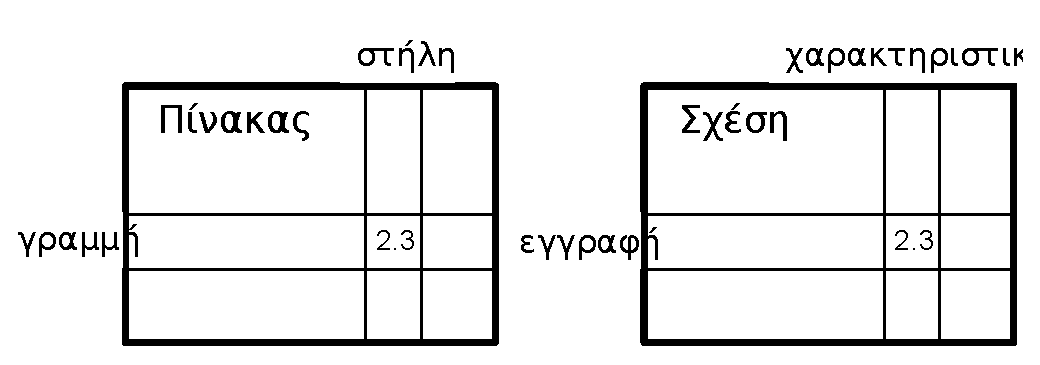
\includegraphics[keepaspectratio,alt={Relational Databases},height=2.0in]{../images/relational.eps}}
\caption{Relational Databases}
\end{figure}

Sa teknikal na mga paglalarawan ng relational databases ang mga konsepto
ng table, row, at column ay mas pormal na tinutukoy bilang
\emph{relation}, \emph{tuple}, at \emph{attribute}, ayon sa
pagkakabanggit. Gagamitin natin ang mas hindi pormal na terms sa chapter
na ito.

\section{Database Browser for SQLite}\label{database-browser-for-sqlite}

Habang ang chapter na ito ay nakatuon sa paggamit ng Python para
magtrabaho sa data sa SQLite database files, maraming operations ay
maaaring gawin nang mas maginhawa gamit ang software na tinatawag na
\emph{Database Browser for SQLite} na libreng available mula sa:

\url{http://sqlitebrowser.org/}

Gamit ang browser maaari mong madaling gumawa ng tables, mag-insert ng
data, mag-edit ng data, o magpatakbo ng simpleng SQL queries sa data sa
database.

Sa isang diwa, ang database browser ay katulad ng text editor kapag
nagtatrabaho sa text files. Kapag gusto mong gumawa ng isa o
napakakaunting operations sa text file, maaari mo lang itong buksan sa
text editor at gawin ang mga pagbabagong gusto mo. Kapag mayroon kang
maraming pagbabago na kailangan mong gawin sa text file, kadalasan
susulat ka ng simpleng Python program. Makikita mo ang parehong pattern
kapag nagtatrabaho sa databases. Gagawa ka ng simpleng operations sa
database manager at mas kumplikadong operations ay pinaka-maginhawang
gawin sa Python.

\section{Creating a database table}\label{creating-a-database-table}

Ang databases ay nangangailangan ng mas tinukoy na structure kaysa sa
Python lists o dictionaries\footnote{Ang SQLite ay talagang
  nagpapahintulot ng ilang flexibility sa uri ng data na naka-store sa
  column, pero pananatilihin natin ang data types natin na strict sa
  chapter na ito para ang concepts ay nalalapat nang pantay sa iba pang
  database systems tulad ng MySQL.}.

Kapag gumagawa tayo ng database \emph{table} dapat nating sabihin sa
database nang maaga ang mga pangalan ng bawat isa sa \emph{columns} sa
table at ang uri ng data na plano nating i-store sa bawat \emph{column}.
Kapag alam ng database software ang uri ng data sa bawat column, maaari
nitong piliin ang pinakamabisang paraan para mag-store at maghanap ng
data batay sa uri ng data.

Maaari mong tingnan ang iba't ibang data types na sinusuportahan ng
SQLite sa sumusunod na url:

\url{http://www.sqlite.org/datatypes.html}

Ang pagtukoy ng structure para sa data mo nang maaga ay maaaring mukhang
hindi maginhawa sa simula, pero ang kapalit ay mabilis na access sa data
mo kahit na ang database ay naglalaman ng malaking dami ng data.

Ang code para gumawa ng database file at table na pinangalanang
\texttt{Track} na may dalawang columns sa database ay ganito:

\index{sqlite3 module} \index{module!sqlite3}

\begin{Shaded}
\begin{Highlighting}[]
\ImportTok{import}\NormalTok{ sqlite3}

\NormalTok{conn }\OperatorTok{=}\NormalTok{ sqlite3.}\ExtensionTok{connect}\NormalTok{(}\StringTok{\textquotesingle{}music.sqlite\textquotesingle{}}\NormalTok{)}
\NormalTok{cur }\OperatorTok{=}\NormalTok{ conn.cursor()}

\NormalTok{cur.execute(}\StringTok{\textquotesingle{}DROP TABLE IF EXISTS Track\textquotesingle{}}\NormalTok{)}
\NormalTok{cur.execute(}\StringTok{\textquotesingle{}CREATE TABLE Track (title TEXT, plays INTEGER)\textquotesingle{}}\NormalTok{)}

\NormalTok{conn.close()}

\CommentTok{\# Code: https://www.py4e.com/code3/db1.py}
\end{Highlighting}
\end{Shaded}

\index{connect function} \index{function!connect}
\index{cursor function} \index{function!cursor}

Ang \texttt{connect} operation ay gumagawa ng ``connection'' sa database
na naka-store sa file na \texttt{music.sqlite} sa current directory.
Kung ang file ay hindi umiiral, gagawin ito. Ang dahilan kung bakit ito
ay tinatawag na ``connection'' ay dahil minsan ang database ay
naka-store sa hiwalay na ``database server'' mula sa server kung saan
tumatakbo ang aming application. Sa simpleng halimbawa natin ang
database ay simpleng local file sa parehong directory ng Python code na
tumatakbo tayo.

Ang \emph{cursor} ay parang file handle na maaari nating gamitin para
gumawa ng operations sa data na naka-store sa database. Ang pagtawag sa
\texttt{cursor()} ay napakatulad conceptually sa pagtawag sa
\texttt{open()} kapag nakikipag-ugnayan sa text files.

\begin{figure}
\centering
\pandocbounded{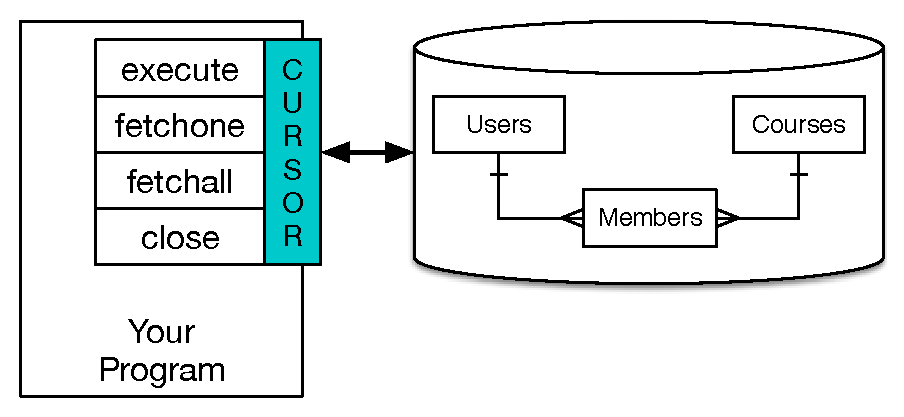
\includegraphics[keepaspectratio,alt={A Database Cursor},height=2.0in]{../images/cursor.eps}}
\caption{A Database Cursor}
\end{figure}

Kapag mayroon na tayong cursor, maaari na tayong magsimulang mag-execute
ng commands sa contents ng database gamit ang \texttt{execute()} method.

Ang database commands ay ipinahayag sa espesyal na language na
na-standardize sa maraming iba't ibang database vendors para payagan
tayong matuto ng isang database language. Ang database language ay
tinatawag na \emph{Structured Query Language} o \emph{SQL} para sa
maikli.

\url{http://en.wikipedia.org/wiki/SQL}

Sa halimbawa natin, nag-e-execute tayo ng dalawang SQL commands sa
database natin. Bilang convention, ipapakita natin ang SQL keywords sa
uppercase at ang mga parte ng command na idinagdag natin (tulad ng table
at column names) ay ipapakita sa lowercase.

Ang unang SQL command ay nagtatanggal ng \texttt{Track} table mula sa
database kung umiiral ito. Ang pattern na ito ay simpleng para payagan
tayong patakbuhin ang parehong program para gumawa ng \texttt{Track}
table nang paulit-ulit nang hindi nagdudulot ng error. Tandaan na ang
\texttt{DROP\ TABLE} command ay nagtatanggal ng table at lahat ng
contents nito mula sa database (i.e., walang ``undo'').

\begin{Shaded}
\begin{Highlighting}[]
\NormalTok{cur.execute(}\StringTok{\textquotesingle{}DROP TABLE IF EXISTS Track \textquotesingle{}}\NormalTok{)}
\end{Highlighting}
\end{Shaded}

Ang pangalawang command ay gumagawa ng table na pinangalanang
\texttt{Track} na may text column na pinangalanang \texttt{title} at
integer column na pinangalanang \texttt{plays}.

\begin{Shaded}
\begin{Highlighting}[]
\NormalTok{cur.execute(}\StringTok{\textquotesingle{}CREATE TABLE Track (title TEXT, plays INTEGER)\textquotesingle{}}\NormalTok{)}
\end{Highlighting}
\end{Shaded}

Ngayon na gumawa na tayo ng table na pinangalanang \texttt{Track},
maaari na tayong maglagay ng ilang data sa table na iyon gamit ang SQL
\texttt{INSERT} operation. Muli, nagsisimula tayo sa pamamagitan ng
paggawa ng connection sa database at pagkuha ng \texttt{cursor}.
Pagkatapos maaari na tayong mag-execute ng SQL commands gamit ang
cursor.

Ang SQL \texttt{INSERT} command ay nagpapahiwatig kung aling table ang
ginagamit natin at pagkatapos nagde-define ng bagong row sa pamamagitan
ng pagli-list ng fields na gusto nating isama \texttt{(title,\ plays)}
na sinusundan ng \texttt{VALUES} na gusto nating ilagay sa bagong row.
Tinutukoy natin ang values bilang question marks \texttt{(?,\ ?)} para
ipahiwatig na ang aktwal na values ay ipinapasa bilang tuple
\texttt{(\ \textquotesingle{}My\ Way\textquotesingle{},\ 15\ )} bilang
pangalawang parameter sa \texttt{execute()} call.

\begin{Shaded}
\begin{Highlighting}[]
\ImportTok{import}\NormalTok{ sqlite3}

\NormalTok{conn }\OperatorTok{=}\NormalTok{ sqlite3.}\ExtensionTok{connect}\NormalTok{(}\StringTok{\textquotesingle{}music.sqlite\textquotesingle{}}\NormalTok{)}
\NormalTok{cur }\OperatorTok{=}\NormalTok{ conn.cursor()}

\NormalTok{cur.execute(}\StringTok{\textquotesingle{}INSERT INTO Track (title, plays) VALUES (?, ?)\textquotesingle{}}\NormalTok{,}
\NormalTok{    (}\StringTok{\textquotesingle{}Thunderstruck\textquotesingle{}}\NormalTok{, }\DecValTok{20}\NormalTok{))}
\NormalTok{cur.execute(}\StringTok{\textquotesingle{}INSERT INTO Track (title, plays) VALUES (?, ?)\textquotesingle{}}\NormalTok{,}
\NormalTok{    (}\StringTok{\textquotesingle{}My Way\textquotesingle{}}\NormalTok{, }\DecValTok{15}\NormalTok{))}
\NormalTok{conn.commit()}

\BuiltInTok{print}\NormalTok{(}\StringTok{\textquotesingle{}Track:\textquotesingle{}}\NormalTok{)}
\NormalTok{cur.execute(}\StringTok{\textquotesingle{}SELECT title, plays FROM Track\textquotesingle{}}\NormalTok{)}
\ControlFlowTok{for}\NormalTok{ row }\KeywordTok{in}\NormalTok{ cur:}
     \BuiltInTok{print}\NormalTok{(row)}

\NormalTok{cur.execute(}\StringTok{\textquotesingle{}DELETE FROM Track WHERE plays \textless{} 100\textquotesingle{}}\NormalTok{)}
\NormalTok{conn.commit()}

\NormalTok{cur.close()}

\CommentTok{\# Code: https://www.py4e.com/code3/db2.py}
\end{Highlighting}
\end{Shaded}

Una nag-\texttt{INSERT} tayo ng dalawang rows sa table natin at
gumagamit ng \texttt{commit()} para pilitin ang data na isulat sa
database file.

\begin{figure}
\centering
\pandocbounded{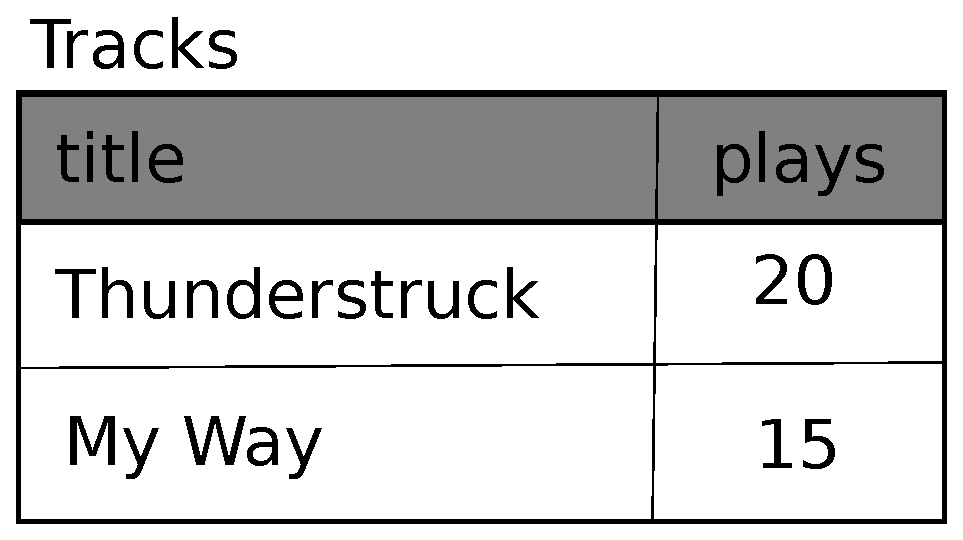
\includegraphics[keepaspectratio,alt={Rows in a Table},height=1.5in]{../images/tracks.eps}}
\caption{Rows in a Table}
\end{figure}

Pagkatapos gumagamit tayo ng \texttt{SELECT} command para kunin ang rows
na kakalagay lang natin mula sa table. Sa \texttt{SELECT} command,
ipinapahiwatig natin kung aling columns ang gusto natin
\texttt{(title,\ plays)} at ipinapahiwatig kung aling table ang gusto
nating kunin ang data. Pagkatapos mag-execute ng \texttt{SELECT}
statement, ang cursor ay isang bagay na maaari nating loop through sa
\texttt{for} statement. Para sa efficiency, ang cursor ay hindi
nagbabasa ng lahat ng data mula sa database kapag nag-e-execute tayo ng
\texttt{SELECT} statement. Sa halip, ang data ay binabasa on demand
habang naglo-loop tayo sa rows sa \texttt{for} statement.

Ang output ng program ay ganito:

{\small
\begin{verbatim}
Track:
('Thunderstruck', 20)
('My Way', 15)
\end{verbatim}
}

\index{Unicode}

Ang \texttt{for} loop natin ay nakakahanap ng dalawang rows, at ang
bawat row ay Python tuple na may unang value bilang \texttt{title} at
pangalawang value bilang bilang ng \texttt{plays}.

Sa pinakadulo ng program, nag-e-execute tayo ng SQL command para
\texttt{DELETE} ang rows na kakalikha lang natin para maaari nating
patakbuhin ang program nang paulit-ulit. Ang \texttt{DELETE} command ay
nagpapakita ng paggamit ng \texttt{WHERE} clause na nagpapahintulot sa
atin na ipahayag ang selection criterion para maaari nating hilingin sa
database na ilapat ang command lang sa rows na tumutugma sa criterion.
Sa halimbawang ito ang criterion ay nalalapat sa lahat ng rows kaya
inu-emptying natin ang table para maaari nating patakbuhin ang program
nang paulit-ulit. Pagkatapos gawin ang \texttt{DELETE}, tumatawag din
tayo sa \texttt{commit()} para pilitin ang data na matanggal mula sa
database.

\section{Structured Query Language
summary}\label{structured-query-language-summary}

\index{CRUD} \index{SQL!CRUD} Hanggang ngayon, gumagamit tayo ng
Structured Query Language sa aming Python examples at natakpan na natin
ang marami sa basics ng SQL commands. Sa section na ito, titingnan natin
ang SQL language partikular at magbigay ng overview ng SQL syntax.

Dahil mayroong napakaraming iba't ibang database vendors, ang Structured
Query Language (SQL) ay na-standardize para maaari tayong
makipag-communicate sa portable na paraan sa database systems mula sa
maraming vendors.

Ang relational database ay binubuo ng tables, rows, at columns. Ang
columns ay karaniwang may type tulad ng text, numeric, o date data.
Kapag gumagawa tayo ng table, ipinapahiwatig natin ang mga pangalan at
uri ng columns:

\begin{Shaded}
\begin{Highlighting}[]
\KeywordTok{CREATE} \KeywordTok{TABLE}\NormalTok{ Track (title TEXT, plays }\DataTypeTok{INTEGER}\NormalTok{)}
\end{Highlighting}
\end{Shaded}

Para mag-insert ng row sa table, gumagamit tayo ng SQL \texttt{INSERT}
command:

\begin{Shaded}
\begin{Highlighting}[]
\KeywordTok{INSERT} \KeywordTok{INTO}\NormalTok{ Track (title, plays) }\KeywordTok{VALUES}\NormalTok{ (}\StringTok{\textquotesingle{}My Way\textquotesingle{}}\NormalTok{, }\DecValTok{15}\NormalTok{)}
\end{Highlighting}
\end{Shaded}

Ang \texttt{INSERT} statement ay nagtutukoy ng table name, pagkatapos
list ng fields/columns na gusto mong i-set sa bagong row, at pagkatapos
ang keyword na \texttt{VALUES} at list ng katumbas na values para sa
bawat field.

Ang SQL \texttt{SELECT} command ay ginagamit para kunin ang rows at
columns mula sa database. Ang \texttt{SELECT} statement ay
nagpapahintulot sa iyo na tukuyin kung aling columns ang gusto mong
kunin pati na rin ang \texttt{WHERE} clause para piliin kung aling rows
ang gusto mong makita. Nagpapahintulot din ito ng opsiyonal na
\texttt{ORDER\ BY} clause para kontrolin ang sorting ng returned rows.

\begin{Shaded}
\begin{Highlighting}[]
\KeywordTok{SELECT} \OperatorTok{*} \KeywordTok{FROM}\NormalTok{ Track }\KeywordTok{WHERE}\NormalTok{ title }\OperatorTok{=} \StringTok{\textquotesingle{}My Way\textquotesingle{}}
\end{Highlighting}
\end{Shaded}

Ang paggamit ng \texttt{*} ay nagpapahiwatig na gusto mong ibalik ng
database ang lahat ng columns para sa bawat row na tumutugma sa
\texttt{WHERE} clause.

Tandaan, hindi tulad sa Python, sa SQL \texttt{WHERE} clause gumagamit
tayo ng isang equal sign para ipahiwatig ang test para sa equality sa
halip na double equal sign. Ang iba pang logical operations na
pinapayagan sa \texttt{WHERE} clause ay kasama ang \texttt{\textless{}},
\texttt{\textgreater{}}, \texttt{\textless{}=},
\texttt{\textgreater{}=}, \texttt{!=}, pati na rin ang \texttt{AND} at
\texttt{OR} at parentheses para gumawa ng logical expressions mo.

Maaari mong hilingin na ang returned rows ay ma-sort ayon sa isa sa
fields tulad ng sumusunod:

\begin{Shaded}
\begin{Highlighting}[]
\KeywordTok{SELECT}\NormalTok{ title,plays }\KeywordTok{FROM}\NormalTok{ Track }\KeywordTok{ORDER} \KeywordTok{BY}\NormalTok{ title}
\end{Highlighting}
\end{Shaded}

Posibleng \texttt{UPDATE} ang column o columns sa loob ng isa o higit
pang rows sa table gamit ang SQL \texttt{UPDATE} statement tulad ng
sumusunod:

\begin{Shaded}
\begin{Highlighting}[]
\KeywordTok{UPDATE}\NormalTok{ Track }\KeywordTok{SET}\NormalTok{ plays }\OperatorTok{=} \DecValTok{16} \KeywordTok{WHERE}\NormalTok{ title }\OperatorTok{=} \StringTok{\textquotesingle{}My Way\textquotesingle{}}
\end{Highlighting}
\end{Shaded}

Ang \texttt{UPDATE} statement ay nagtutukoy ng table at pagkatapos list
ng fields at values na baguhin pagkatapos ng \texttt{SET} keyword at
pagkatapos opsiyonal na \texttt{WHERE} clause para piliin ang rows na
dapat i-update. Ang isang \texttt{UPDATE} statement ay magbabago ng
lahat ng rows na tumutugma sa \texttt{WHERE} clause. Kung ang
\texttt{WHERE} clause ay hindi tinukoy, ginagawa nito ang
\texttt{UPDATE} sa lahat ng rows sa table.

Para tanggalin ang row, kailangan mo ng \texttt{WHERE} clause sa SQL
\texttt{DELETE} statement. Ang \texttt{WHERE} clause ay nagde-determine
kung aling rows ang dapat tanggalin:

\begin{Shaded}
\begin{Highlighting}[]
\KeywordTok{DELETE} \KeywordTok{FROM}\NormalTok{ Track }\KeywordTok{WHERE}\NormalTok{ title }\OperatorTok{=} \StringTok{\textquotesingle{}My Way\textquotesingle{}}
\end{Highlighting}
\end{Shaded}

\index{CRUD} \index{SQL!CRUD} Ang apat na basic SQL commands na ito
(INSERT, SELECT, UPDATE, at DELETE) ay nagpapahintulot sa apat na basic
operations na kailangan para gumawa at mag-maintain ng data. Gumagamit
tayo ng ``CRUD'' (Create, Read, Update, at Delete) para makuha ang lahat
ng concepts na ito sa isang term.\footnote{Oo may disconnect sa pagitan
  ng ``CRUD'' term at unang letters ng apat na SQL statements na
  nag-i-implement ng ``CRUD''. Ang posibleng paliwanag ay maaaring
  sabihin na ang ``CRUD'' ay ang ``concept'' at ang SQL ay ang
  implementation. Ang isa pang posibleng paliwanag ay mas masaya sabihin
  ang ``CRUD'' kaysa sa ``ISUD''.}

\section{Multiple tables and basic data
modeling}\label{multiple-tables-and-basic-data-modeling}

\index{Data Modelling} \index{Relational Model} Ang tunay na
kapangyarihan ng relational database ay kapag gumagawa tayo ng maraming
tables at gumagawa ng links sa pagitan ng mga tables na iyon. Ang gawain
ng pagde-decide kung paano hatiin ang application data mo sa maraming
tables at pagtatatag ng relationships sa pagitan ng tables ay tinatawag
na \emph{data modeling}. Ang design document na nagpapakita ng tables at
kanilang relationships ay tinatawag na \emph{data model}.

Ang data modeling ay relatively sophisticated skill at ipakikilala lang
natin ang pinakabasic concepts ng relational data modeling sa section na
ito. Para sa mas detalyado tungkol sa data modeling maaari kang
magsimula sa:

\url{http://en.wikipedia.org/wiki/Relational_model}

\index{SQL!CREATE} Sabihin natin para sa tracks database natin gusto
nating i-track ang pangalan ng \texttt{artist} para sa bawat track
bilang karagdagan sa \texttt{title} at bilang ng plays para sa bawat
track. Ang simpleng approach ay maaaring simpleng magdagdag ng iba pang
column sa database na tinatawag na \texttt{artist} at ilagay ang
pangalan ng artist sa column tulad ng sumusunod:

\begin{Shaded}
\begin{Highlighting}[]
\NormalTok{DROP TABLE IF EXISTS Track}\OperatorTok{;}
\NormalTok{CREATE TABLE Track (title TEXT, plays INTEGER, artist TEXT)}\OperatorTok{;}
\end{Highlighting}
\end{Shaded}

Pagkatapos maaari tayong mag-insert ng ilang tracks sa table natin.

\begin{Shaded}
\begin{Highlighting}[]
\KeywordTok{INSERT} \KeywordTok{INTO}\NormalTok{ Track (title, plays, artist)}
    \KeywordTok{VALUES}\NormalTok{ (}\StringTok{\textquotesingle{}My Way\textquotesingle{}}\NormalTok{, }\DecValTok{15}\NormalTok{, }\StringTok{\textquotesingle{}Frank Sinatra\textquotesingle{}}\NormalTok{);}
\KeywordTok{INSERT} \KeywordTok{INTO}\NormalTok{ Track (title, plays, artist)}
    \KeywordTok{VALUES}\NormalTok{ (}\StringTok{\textquotesingle{}New York\textquotesingle{}}\NormalTok{, }\DecValTok{25}\NormalTok{, }\StringTok{\textquotesingle{}Frank Sinatra\textquotesingle{}}\NormalTok{);}
\end{Highlighting}
\end{Shaded}

Kung titingnan natin ang data natin gamit ang
\texttt{SELECT\ *\ FROM\ Track} statement, mukhang maganda ang ginawa
natin.

{\small
\begin{verbatim}
sqlite> SELECT * FROM Track;
My Way|15|Frank Sinatra
New York|25|Frank Sinatra
sqlite>
\end{verbatim}
}

Gumawa tayo ng \emph{napakasamang error} sa data modeling natin. Nilabag
natin ang rules ng \emph{database normalization}.

\url{https://en.wikipedia.org/wiki/Database_normalization}

\index{Database Normalization} \index{Data Normalization} Habang ang
database normalization ay mukhang napakakumplikado sa ibabaw at
naglalaman ng maraming mathematical justifications, sa ngayon maaari
nating bawasan ang lahat sa isang simpleng rule na susundin natin.

\index{Data Replication} Hindi dapat nating ilagay ang parehong string
data sa column nang higit sa isang beses. Kung kailangan natin ang data
nang higit sa isang beses, gumagawa tayo ng numeric \emph{key} para sa
data at nagre-reference sa aktwal na data gamit ang key na ito. Lalo na
kung ang maraming entries ay tumutukoy sa parehong object.

Para ipakita ang slippery slope na binababa natin sa pamamagitan ng
pag-assign ng string columns sa database model natin, isipin kung paano
natin babaguhin ang data model kung gusto nating i-track ang eye color
ng artists natin? Gagawin ba natin ito?

\begin{Shaded}
\begin{Highlighting}[]
\KeywordTok{DROP} \KeywordTok{TABLE} \ControlFlowTok{IF} \KeywordTok{EXISTS}\NormalTok{ Track;}
\KeywordTok{CREATE} \KeywordTok{TABLE}\NormalTok{ Track (title TEXT, plays }\DataTypeTok{INTEGER}\NormalTok{,}
\NormalTok{    artist TEXT, eyes TEXT);}
\KeywordTok{INSERT} \KeywordTok{INTO}\NormalTok{ Track (title, plays, artist, eyes)}
    \KeywordTok{VALUES}\NormalTok{ (}\StringTok{\textquotesingle{}My Way\textquotesingle{}}\NormalTok{, }\DecValTok{15}\NormalTok{, }\StringTok{\textquotesingle{}Frank Sinatra\textquotesingle{}}\NormalTok{, }\StringTok{\textquotesingle{}Blue\textquotesingle{}}\NormalTok{);}
\KeywordTok{INSERT} \KeywordTok{INTO}\NormalTok{ Track (title, plays, artist, eyes)}
    \KeywordTok{VALUES}\NormalTok{ (}\StringTok{\textquotesingle{}New York\textquotesingle{}}\NormalTok{, }\DecValTok{25}\NormalTok{, }\StringTok{\textquotesingle{}Frank Sinatra\textquotesingle{}}\NormalTok{, }\StringTok{\textquotesingle{}Blue\textquotesingle{}}\NormalTok{);}
\end{Highlighting}
\end{Shaded}

Dahil nag-record si Frank Sinatra ng higit sa 1200 songs, talaga bang
ilalagay natin ang string na `Blue' sa 1200 rows sa \texttt{Track} table
natin. At ano ang mangyayari kung magde-decide tayo na ang eye color
niya ay `Light Blue'? May bagay na hindi tama.

Ang tamang solusyon ay gumawa ng table para sa bawat \texttt{Artist} at
mag-store ng lahat ng data tungkol sa artist sa table na iyon. At
pagkatapos kailangan nating gumawa ng connection sa pagitan ng row sa
\texttt{Track} table patungo sa row sa \texttt{Artist} table. Marahil
maaari nating tawagin ang ``link'' na ito sa pagitan ng dalawang
``tables'' na ``relationship'' sa pagitan ng dalawang tables. At iyon
mismo ang napagpasyahan ng database experts na tawagin sa lahat ng mga
links na ito.

Gumawa tayo ng \texttt{Artist} table tulad ng sumusunod:

\begin{Shaded}
\begin{Highlighting}[]
\KeywordTok{DROP} \KeywordTok{TABLE} \ControlFlowTok{IF} \KeywordTok{EXISTS}\NormalTok{ Artist;}
\KeywordTok{CREATE} \KeywordTok{TABLE}\NormalTok{ Artist (name TEXT, eyes TEXT);}
\KeywordTok{INSERT} \KeywordTok{INTO}\NormalTok{ Artist (name, eyes)}
   \KeywordTok{VALUES}\NormalTok{ (}\StringTok{\textquotesingle{}Frank Sinatra\textquotesingle{}}\NormalTok{, }\StringTok{\textquotesingle{}blue\textquotesingle{}}\NormalTok{);}
\end{Highlighting}
\end{Shaded}

\index{primary key} Ngayon mayroon tayong dalawang tables pero kailangan
natin ng paraan para \emph{i-link} ang rows sa dalawang tables. Para
gawin ito, kailangan natin ng tinatawag nating `keys'. Ang mga keys na
ito ay simpleng integer numbers na maaari nating gamitin para maghanap
ng row sa iba't ibang table. Kung gagawa tayo ng links sa rows sa loob
ng table, kailangan nating magdagdag ng \emph{primary key} sa rows sa
table. Ayon sa convention karaniwang pinapangalanan natin ang primary
key column na `id'. Kaya ang \texttt{Artist} table natin ay ganito:

\begin{Shaded}
\begin{Highlighting}[]
\KeywordTok{DROP} \KeywordTok{TABLE} \ControlFlowTok{IF} \KeywordTok{EXISTS}\NormalTok{ Artist;}
\KeywordTok{CREATE} \KeywordTok{TABLE}\NormalTok{ Artist (}\KeywordTok{id} \DataTypeTok{INTEGER}\NormalTok{, name TEXT, eyes TEXT);}
\KeywordTok{INSERT} \KeywordTok{INTO}\NormalTok{ Artist (}\KeywordTok{id}\NormalTok{, name, eyes)}
   \KeywordTok{VALUES}\NormalTok{ (}\DecValTok{42}\NormalTok{, }\StringTok{\textquotesingle{}Frank Sinatra\textquotesingle{}}\NormalTok{, }\StringTok{\textquotesingle{}blue\textquotesingle{}}\NormalTok{);}
\end{Highlighting}
\end{Shaded}

Ngayon mayroon tayong row sa table para sa `Frank Sinatra' (at eye color
niya) at primary key na `42' para gamitin para i-link ang tracks natin
sa kanya. Kaya binabago natin ang Track table natin tulad ng sumusunod:

\begin{Shaded}
\begin{Highlighting}[]
\KeywordTok{DROP} \KeywordTok{TABLE} \ControlFlowTok{IF} \KeywordTok{EXISTS}\NormalTok{ Track;}
\KeywordTok{CREATE} \KeywordTok{TABLE}\NormalTok{ Track (title TEXT, plays }\DataTypeTok{INTEGER}\NormalTok{,}
\NormalTok{    artist\_id }\DataTypeTok{INTEGER}\NormalTok{);}
\KeywordTok{INSERT} \KeywordTok{INTO}\NormalTok{ Track (title, plays, artist\_id)}
    \KeywordTok{VALUES}\NormalTok{ (}\StringTok{\textquotesingle{}My Way\textquotesingle{}}\NormalTok{, }\DecValTok{15}\NormalTok{, }\DecValTok{42}\NormalTok{);}
\KeywordTok{INSERT} \KeywordTok{INTO}\NormalTok{ Track (title, plays, artist\_id)}
    \KeywordTok{VALUES}\NormalTok{ (}\StringTok{\textquotesingle{}New York\textquotesingle{}}\NormalTok{, }\DecValTok{25}\NormalTok{, }\DecValTok{42}\NormalTok{);}
\end{Highlighting}
\end{Shaded}

\index{Foreign key} Ang \texttt{artist\_id} column ay integer, at ayon
sa naming convention ay \emph{foreign key} na tumuturo sa \emph{primary}
key sa \texttt{Artist} table. Tinatawag natin itong foreign key dahil
tumuturo ito sa row sa iba't ibang table.

\index{SQL!JOIN} \index{SQL!ON} Ngayon sumusunod na tayo sa rules ng
database normalization, pero kapag gusto nating makuha ang data mula sa
database natin, hindi natin gusto na makita ang 42, gusto nating makita
ang pangalan at eye color ng artist. Para gawin ito gumagamit tayo ng
keyword na \texttt{JOIN} sa SELECT statement natin.

\begin{Shaded}
\begin{Highlighting}[]
\KeywordTok{SELECT}\NormalTok{ title, plays, name, eyes}
\KeywordTok{FROM}\NormalTok{ Track }\KeywordTok{JOIN}\NormalTok{ Artist}
\KeywordTok{ON}\NormalTok{ Track.artist\_id }\OperatorTok{=}\NormalTok{ Artist.}\KeywordTok{id}\NormalTok{;}
\end{Highlighting}
\end{Shaded}

Ang \texttt{JOIN} clause ay kasama ang \texttt{ON} condition na
nagde-define kung paano ang rows ay dapat konektado. Para sa bawat row
sa \texttt{Track} idagdag ang data mula sa \texttt{Artist} mula sa row
kung saan ang \texttt{artist\_id} sa \texttt{Track} table ay tumutugma
sa \texttt{id} mula sa \texttt{Artist} table.

Ang output ay magiging:

{\small
\begin{verbatim}
My Way|15|Frank Sinatra|blue
New York|25|Frank Sinatra|blue
\end{verbatim}
}

Habang maaaring mukhang medyo clunky at ang instincts mo ay maaaring
sabihin sa iyo na mas mabilis lang na panatilihin ang data sa isang
table, lumalabas na ang limit sa database performance ay kung gaano
karaming data ang kailangang i-scan kapag kumukuha ng query. Habang ang
detalye ay napakakumplikado, ang integers ay mas maliit kaysa sa strings
(lalo na ang Unicode) at mas mabilis na ilipat at i-compare.

\section{Data model diagrams}\label{data-model-diagrams}

\index{Data model diagrams} \index{Entity-Relationship diagrams} Habang
ang \texttt{Track} at \texttt{Artist} database design natin ay simple na
may dalawang tables lang at isang one-to-many relationship, ang mga data
models na ito ay maaaring maging kumplikado nang mabilis at mas madaling
maintindihan kung maaari tayong gumawa ng graphical representation ng
data model natin.

\begin{figure}
\centering
\pandocbounded{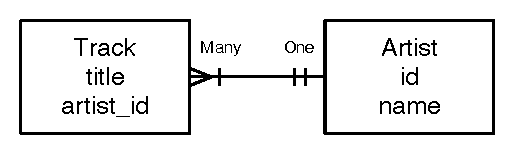
\includegraphics[keepaspectratio,alt={A Verbose One-to-Many Data Model},height=1.5in]{../images/one-to-many-verbose.eps}}
\caption{A Verbose One-to-Many Data Model\label{figvrbo2m}}
\end{figure}

\index{Crow's Foot diagrams} While there are many graphical
representations of data models, we will use one of the ``classic''
approaches, called ``Crow's Foot Diagrams'' as shown in Figure
\ref{figvrbo2m}. Each table is shown as a box with the name of the table
and its columns. Then where there is a relationship between two tables a
line is drawn connecting the tables with a notation added to the end of
each line indicating the nature of the relationship.

\url{https://en.wikipedia.org/wiki/Entity-relationship_model}

In this case, ``many'' tracks can be associated with each artist. So the
track end is shown with the crow's foot spread out indicating it is
the'' ``many'' end. The artist end is shown with a vertical like that
indicates ``one''. There will be ``many'' artists in general, but the
important aspect is that for each artist there will be many tracks. And
each of those artists may be associated with multiple tracks.

\index{foreign key} You will note that the column that holds the
\emph{foreign\_key} like \texttt{artist\_id} is on the ``many'' end and
the \emph{primary key} is at the ``one'' end.

Since the pattern of foreign and primary key placement is so consistent
and follows the ``many'' and ``one'' ends of the lines, we never include
either the primary or foreign key columns in our diagram of the data
model as shown in the second diagram as shown in Figure \ref{figo2m}.
The columns are thought of as ``implementation detail'' to capture the
nature of the relationship details and not an essential part of the data
being modeled.

\begin{figure}
\centering
\pandocbounded{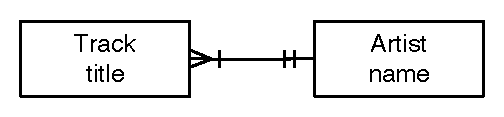
\includegraphics[keepaspectratio,alt={A Succinct One-to-Many Data Model},height=1.5in]{../images/one-to-many.eps}}
\caption{A Succinct One-to-Many Data Model\label{figo2m}}
\end{figure}

\section{Automatically creating primary
keys}\label{automatically-creating-primary-keys}

\index{Primary key} \index{Auto increment} \index{SQL!UNIQUE} In the
above example, we arbitrarily assigned Frank the primary key of 42.
However when we are inserting millions or rows, it is nice to have the
database automatically generate the values for the id column. We do this
by declaring the \texttt{id} column as a \texttt{PRIMARY\ KEY} and leave
out the \texttt{id} value when inserting the row:

\begin{Shaded}
\begin{Highlighting}[]
\KeywordTok{DROP} \KeywordTok{TABLE} \ControlFlowTok{IF} \KeywordTok{EXISTS}\NormalTok{ Artist;}
\KeywordTok{CREATE} \KeywordTok{TABLE}\NormalTok{ Artist (}\KeywordTok{id} \DataTypeTok{INTEGER} \KeywordTok{PRIMARY} \KeywordTok{KEY}\NormalTok{,}
\NormalTok{    name TEXT, eyes TEXT);}
\KeywordTok{INSERT} \KeywordTok{INTO}\NormalTok{ Artist (name, eyes)}
   \KeywordTok{VALUES}\NormalTok{ (}\StringTok{\textquotesingle{}Frank Sinatra\textquotesingle{}}\NormalTok{, }\StringTok{\textquotesingle{}blue\textquotesingle{}}\NormalTok{);}
\end{Highlighting}
\end{Shaded}

Now we have instructed the database to auto-assign us a unique value to
the Frank Sinatra row. But we then need a way to have the database tell
us the \texttt{id} value for the recently inserted row. One way is to
use a \texttt{SELECT} statement to retrieve data from an SQLite
built-in-function called \texttt{last\_insert\_rowid()}.

{\small
\begin{verbatim}
sqlite> DROP TABLE IF EXISTS Artist;
sqlite> CREATE TABLE Artist (id INTEGER PRIMARY KEY,
   ...>     name TEXT, eyes TEXT);
sqlite> INSERT INTO Artist (name, eyes)
   ...>    VALUES ('Frank Sinatra', 'blue');
sqlite> select last_insert_rowid();
1
sqlite> SELECT * FROM Artist;
1|Frank Sinatra|blue
sqlite>
\end{verbatim}
}

Once we know the \texttt{id} of our `Frank Sinatra' row, we can use it
when we \texttt{INSERT} the tracks into the \texttt{Track} table. As a
general strategy, we add these \texttt{id} columns to any table we
create:

{\small
\begin{verbatim}
sqlite> DROP TABLE IF EXISTS Track;
sqlite> CREATE TABLE Track (id INTEGER PRIMARY KEY,
   ...>     title TEXT, plays INTEGER, artist_id INTEGER);
\end{verbatim}
}

Note that the \texttt{artist\_id} value is the new auto-assigned row in
the \texttt{Artist} table and that while we added an
\texttt{INTEGER\ PRIMARY\ KEY} to the \texttt{Track} table, we did not
include \texttt{id} in the list of fields on the \texttt{INSERT}
statements into the \texttt{Track} table. Again this tells the database
to choose a unique value for us for the \texttt{id} column.

{\small
\begin{verbatim}
sqlite> INSERT INTO Track (title, plays, artist_id)
   ...>     VALUES ('My Way', 15, 1);
sqlite> select last_insert_rowid();
1
sqlite> INSERT INTO Track (title, plays, artist_id)
   ...>     VALUES ('New York', 25, 1);
sqlite> select last_insert_rowid();
2
sqlite>
\end{verbatim}
}

\index{Primary key retrieval} You can call
\texttt{SELECT\ last\_insert\_rowid();} after each of the inserts to
retrieve the value that the database assigned to the \texttt{id} of each
newly created row. Later when we are coding in Python, we can ask for
the \texttt{id} value in our code and store it in a variable for later
use.

\section{Logical keys for fast
lookup}\label{logical-keys-for-fast-lookup}

\index{Logical key} \index{SQL!INDEX} If we had a table full of artists
and a table full of tracks, each with a foreign key link to a row in a
table full of artists and we wanted to list all the tracks that were
sung by `Frank Sinatra' as follows:

{\small
\begin{verbatim}
SELECT title, plays, name, eyes
FROM Track JOIN Artist
ON Track.artist_id = Artist.id
WHERE Artist.name = 'Frank Sinatra';
\end{verbatim}
}

Since we have two tables and a foreign key between the two tables, our
data is well-modeled, but if we are going to have millions of records in
the \texttt{Artist} table and going to do a lot of lookups by artist
name, we would benefit if we gave the database a hint about our intended
use of the \texttt{name} column.

\index{CREATE INDEX} We do this by adding an ``index'' to a text column
that we intend to use in \texttt{WHERE} clauses:

{\small
\begin{verbatim}
CREATE INDEX artist_name ON Artist(name);
\end{verbatim}
}

When the database has been told that an index is needed on a column in a
table, it stores extra information to make it possible to look up a row
more quickly using the indexed field (\texttt{name} in this example).
Once you request that an index be created, there is nothing special that
is needed in the SQL to access the table. The database keeps the index
up to date as data is inserted, deleted, and updated, and uses it
automatically if it will increase the performance of a database query.

These text columns that are used to find rows based on some information
in the ``real world'' like the name of an artist are called
\emph{Logical keys}.

\section{Adding constraints to the
database}\label{adding-constraints-to-the-database}

\index{Constraint} \index{SQL!UNIQUE} We can also use an index to
enforce a constraint (i.e.~rules) on our database operations. The most
common constraint is a \emph{uniqueness constraint} which insists that
all of the values in a column are unique. We can add the optional
\texttt{UNIQUE} keyword, to the \texttt{CREATE\ INDEX} statement to tell
the database that we would like it to enforce the constraint on our SQL.
We can drop and re-create the \texttt{artist\_name} index with a
\texttt{UNIQUE} constraint as follows.

{\small
\begin{verbatim}
DROP INDEX artist_name;
CREATE UNIQUE INDEX artist_name ON Artist(name);
\end{verbatim}
}

If we try to insert `Frank Sinatra' a second time, it will fail with an
error.

{\small
\begin{verbatim}
sqlite> SELECT * FROM Artist;
1|Frank Sinatra|blue
sqlite> INSERT INTO Artist (name, eyes)
   ...>    VALUES ('Frank Sinatra', 'blue');
Runtime error: UNIQUE constraint failed: Artist.name (19)
sqlite>
\end{verbatim}
}

\index{SQL!IGNORE} We can tell the database to ignore any duplicate key
errors by adding the \texttt{IGNORE} keyword to the \texttt{INSERT}
statement as follows:

{\small
\begin{verbatim}
sqlite> INSERT OR IGNORE INTO Artist (name, eyes)
   ...>     VALUES ('Frank Sinatra', 'blue');
sqlite> SELECT id FROM Artist WHERE name='Frank Sinatra';
1
sqlite>
\end{verbatim}
}

By combining an \texttt{INSERT\ OR\ IGNORE} and a \texttt{SELECT} we can
insert a new record if the name is not already there and whether or not
the record is already there, retrieve the \emph{primary} key of the
record.

{\small
\begin{verbatim}
sqlite> INSERT OR IGNORE INTO Artist (name, eyes)
   ...>      VALUES ('Elvis', 'blue');
sqlite> SELECT id FROM Artist WHERE name='Elvis';
2
sqlite> SELECT * FROM Artist;
1|Frank Sinatra|blue
2|Elvis|blue
sqlite>
\end{verbatim}
}

Since we have not added a uniqueness constraint to the eye color column,
there is no problem having multiple `Blue' values in the \texttt{eye}
column.

\begin{figure}
\centering
\pandocbounded{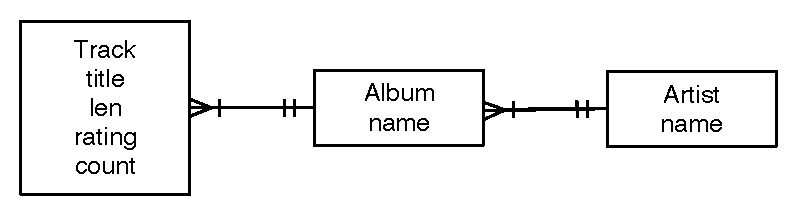
\includegraphics[keepaspectratio,alt={Tracks, Albums, and Artists},height=1.5in]{../images/tracks-albums-artists.eps}}
\caption{Tracks, Albums, and Artists\label{figtaa}}
\end{figure}

\section{Sample multi-table
application}\label{sample-multi-table-application}

A sample application called \texttt{tracks\_csv.py} shows how these
ideas can be combined to parse textual data and load it into several
tables using a proper data model with relational connections between the
tables.

This application reads and parses a comma-separated file
\texttt{tracks.csv} based on an export from Dr.~Chuck's iTunes library.

{\small
\begin{verbatim}
Another One Bites The Dust,Queen,Greatest Hits,55,100,217103
Asche Zu Asche,Rammstein,Herzeleid,79,100,231810
Beauty School Dropout,Various,Grease,48,100,239960
Black Dog,Led Zeppelin,IV,109,100,296620
...
\end{verbatim}
}

The columns in this file are: title, artist, album, number of plays,
rating (0-100) and length in milliseconds.

Our data model is shown in Figure \ref{figtaa} and described in SQL as
follows:

\begin{Shaded}
\begin{Highlighting}[]
\KeywordTok{DROP} \KeywordTok{TABLE} \ControlFlowTok{IF} \KeywordTok{EXISTS}\NormalTok{ Artist;}
\KeywordTok{DROP} \KeywordTok{TABLE} \ControlFlowTok{IF} \KeywordTok{EXISTS}\NormalTok{ Album;}
\KeywordTok{DROP} \KeywordTok{TABLE} \ControlFlowTok{IF} \KeywordTok{EXISTS}\NormalTok{ Track;}

\KeywordTok{CREATE} \KeywordTok{TABLE}\NormalTok{ Artist (}
    \KeywordTok{id} \DataTypeTok{INTEGER} \KeywordTok{PRIMARY} \KeywordTok{KEY}\NormalTok{,}
\NormalTok{    name TEXT }\KeywordTok{UNIQUE}
\NormalTok{);}

\KeywordTok{CREATE} \KeywordTok{TABLE}\NormalTok{ Album (}
    \KeywordTok{id} \DataTypeTok{INTEGER} \KeywordTok{PRIMARY} \KeywordTok{KEY}\NormalTok{,}
\NormalTok{    artist\_id  }\DataTypeTok{INTEGER}\NormalTok{,}
\NormalTok{    title TEXT }\KeywordTok{UNIQUE}
\NormalTok{);}

\KeywordTok{CREATE} \KeywordTok{TABLE}\NormalTok{ Track (}
    \KeywordTok{id} \DataTypeTok{INTEGER} \KeywordTok{PRIMARY} \KeywordTok{KEY}\NormalTok{,}
\NormalTok{    title TEXT }\KeywordTok{UNIQUE}\NormalTok{,}
\NormalTok{    album\_id }\DataTypeTok{INTEGER}\NormalTok{,}
\NormalTok{    len }\DataTypeTok{INTEGER}\NormalTok{, rating }\DataTypeTok{INTEGER}\NormalTok{, }\FunctionTok{count} \DataTypeTok{INTEGER}
\NormalTok{);}
\end{Highlighting}
\end{Shaded}

We are adding the \texttt{UNIQUE} keyword to \texttt{TEXT} columns that
we would like to have a uniqueness constraint that we will use in
\texttt{INSERT\ IGNORE} statements. This is more succinct than separate
\texttt{CREATE\ INDEX} statements but has the same effect.

With these tables in place, we write the following code
\texttt{tracks\_csv.py} to parse the data and insert it into the tables:

\begin{Shaded}
\begin{Highlighting}[]
\ImportTok{import}\NormalTok{ sqlite3}

\NormalTok{conn }\OperatorTok{=}\NormalTok{ sqlite3.}\ExtensionTok{connect}\NormalTok{(}\StringTok{\textquotesingle{}trackdb.sqlite\textquotesingle{}}\NormalTok{)}
\NormalTok{cur }\OperatorTok{=}\NormalTok{ conn.cursor()}

\NormalTok{handle }\OperatorTok{=} \BuiltInTok{open}\NormalTok{(}\StringTok{\textquotesingle{}tracks.csv\textquotesingle{}}\NormalTok{)}

\ControlFlowTok{for}\NormalTok{ line }\KeywordTok{in}\NormalTok{ handle:}
\NormalTok{    line }\OperatorTok{=}\NormalTok{ line.strip()}\OperatorTok{;}
\NormalTok{    pieces }\OperatorTok{=}\NormalTok{ line.split(}\StringTok{\textquotesingle{},\textquotesingle{}}\NormalTok{)}
    \ControlFlowTok{if} \BuiltInTok{len}\NormalTok{(pieces) }\OperatorTok{!=} \DecValTok{6}\NormalTok{ : }\ControlFlowTok{continue}

\NormalTok{    name }\OperatorTok{=}\NormalTok{ pieces[}\DecValTok{0}\NormalTok{]}
\NormalTok{    artist }\OperatorTok{=}\NormalTok{ pieces[}\DecValTok{1}\NormalTok{]}
\NormalTok{    album }\OperatorTok{=}\NormalTok{ pieces[}\DecValTok{2}\NormalTok{]}
\NormalTok{    count }\OperatorTok{=}\NormalTok{ pieces[}\DecValTok{3}\NormalTok{]}
\NormalTok{    rating }\OperatorTok{=}\NormalTok{ pieces[}\DecValTok{4}\NormalTok{]}
\NormalTok{    length }\OperatorTok{=}\NormalTok{ pieces[}\DecValTok{5}\NormalTok{]}

    \BuiltInTok{print}\NormalTok{(name, artist, album, count, rating, length)}

\NormalTok{    cur.execute(}\StringTok{\textquotesingle{}\textquotesingle{}\textquotesingle{}INSERT OR IGNORE INTO Artist (name)}
\StringTok{        VALUES ( ? )\textquotesingle{}\textquotesingle{}\textquotesingle{}}\NormalTok{, ( artist, ) )}
\NormalTok{    cur.execute(}\StringTok{\textquotesingle{}SELECT id FROM Artist WHERE name = ? \textquotesingle{}}\NormalTok{, (artist, ))}
\NormalTok{    artist\_id }\OperatorTok{=}\NormalTok{ cur.fetchone()[}\DecValTok{0}\NormalTok{]}

\NormalTok{    cur.execute(}\StringTok{\textquotesingle{}\textquotesingle{}\textquotesingle{}INSERT OR IGNORE INTO Album (title, artist\_id)}
\StringTok{        VALUES ( ?, ? )\textquotesingle{}\textquotesingle{}\textquotesingle{}}\NormalTok{, ( album, artist\_id ) )}
\NormalTok{    cur.execute(}\StringTok{\textquotesingle{}SELECT id FROM Album WHERE title = ? \textquotesingle{}}\NormalTok{, (album, ))}
\NormalTok{    album\_id }\OperatorTok{=}\NormalTok{ cur.fetchone()[}\DecValTok{0}\NormalTok{]}

\NormalTok{    cur.execute(}\StringTok{\textquotesingle{}\textquotesingle{}\textquotesingle{}INSERT OR REPLACE INTO Track}
\StringTok{        (title, album\_id, len, rating, count)}
\StringTok{        VALUES ( ?, ?, ?, ?, ? )\textquotesingle{}\textquotesingle{}\textquotesingle{}}\NormalTok{,}
\NormalTok{        ( name, album\_id, length, rating, count ) )}

\NormalTok{    conn.commit()}
\end{Highlighting}
\end{Shaded}

You can see that we are repeating the pattern of
\texttt{INSERT\ OR\ IGNORE} followed by a \texttt{SELECT} to get the
appropriate \texttt{artist\_id} and \texttt{album\_id} for use in later
\texttt{INSERT} statements. We start from \texttt{Artist} because we
need \texttt{artist\_id} to insert the \texttt{Album} and need the
\texttt{album\_id} to insert the \texttt{Track}.

\index{Primary key} \index{Foreign key} If we look at the \texttt{Album}
table, we can see that the entries were added and assigned a
\emph{primary} key as necessary as the data was parsed. We can also see
the \emph{foreign key} pointing to a row in the \texttt{Artist} table
for each \texttt{Album} row.

{\small
\begin{verbatim}
sqlite> .mode column
sqlite> SELECT * FROM Album LIMIT 5;
id  artist_id  title 
--  ---------  -----------------
1   1          Greatest Hits    
2   2          Herzeleid        
3   3          Grease           
4   4          IV               
5   5          The Wall [Disc 2]
\end{verbatim}
}

\index{SQL!JOIN} \index{SQL!ON} We can reconstruct all of the
\texttt{Track} data, following all the relations using
\texttt{JOIN\ /\ ON} clauses. You can see both ends of each of the (2)
relational connections in each row in the output below:

{\small
\begin{verbatim}
sqlite> .mode line
sqlite> SELECT * FROM Track
   ...> JOIN Album ON Track.album_id = Album.id
   ...> JOIN Artist ON Album.artist_id = Artist.id
   ...> LIMIT 2;
       id = 1
    title = Another One Bites The Dust
 album_id = 1
      len = 217103
   rating = 100
    count = 55
       id = 1
artist_id = 1
    title = Greatest Hits
       id = 1
     name = Queen

       id = 2
    title = Asche Zu Asche
 album_id = 2
      len = 231810
   rating = 100
    count = 79
       id = 2
artist_id = 2
    title = Herzeleid
       id = 2
     name = Rammstein
\end{verbatim}
}

This example shows three tables and two \emph{one-to-many} relationships
between the tables. It also shows how to use indexes and uniqueness
constraints to programmatically construct the tables and their
relationships.

\url{https://en.wikipedia.org/wiki/One-to-many_(data_model)}

Up next we will look at the many-to-many relationships in data models.

\section{Many to many relationships in
databases}\label{many-to-many-relationships-in-databases}

\index{Data model} \index{Many to many relationship}
\index{Crow's foot diagram} Some data relationships cannot be modeled by
a simple one-to-many relationship. For example, lets say we are going to
build a data model for a course management system. There will be
courses, users, and rosters. A user can be on the roster for many
courses and a course will have many users on its roster.

It is pretty simple to \emph{draw} a many-to-many relationship as shown
in Figure \ref{figm2m}. We simply draw two tables and connect them with
a line that has the ``many'' indicator on both ends of the lines. The
problem is how to \emph{implement} the relationship using primary keys
and foreign keys.

Before we explore how we implement many-to-many relationships, let's see
if we could hack something up by extending a one-to many relationship.

\begin{figure}
\centering
\pandocbounded{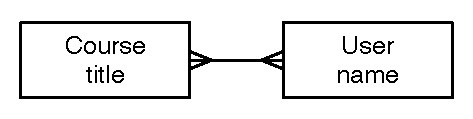
\includegraphics[keepaspectratio,alt={A Many to Many Relationship},height=1.5in]{../images/many-to-many.eps}}
\caption{A Many to Many Relationship\label{figm2m}}
\end{figure}

If SQL supported the notion of arrays, we might try to define this:

\begin{Shaded}
\begin{Highlighting}[]
\KeywordTok{CREATE} \KeywordTok{TABLE}\NormalTok{ Course (}
    \KeywordTok{id}     \DataTypeTok{INTEGER} \KeywordTok{PRIMARY} \KeywordTok{KEY}\NormalTok{,}
\NormalTok{    title  TEXT }\KeywordTok{UNIQUE}
\NormalTok{    student\_ids }\DataTypeTok{ARRAY} \KeywordTok{OF} \DataTypeTok{INTEGER}\NormalTok{;}
\NormalTok{);}
\end{Highlighting}
\end{Shaded}

Sadly, while this is a tempting idea, SQL does not support
arrays.\footnote{Some SQL dialects support arrays but arrays do not
  scale well. NoSQL databases use arrays and data replication but at a
  cost of database integrity. NoSQL is a story for another course
  https://www.pg4e.com/}

Or we could just make long string and concatenate all the \texttt{User}
primary keys into a long string separated by commas.

\begin{Shaded}
\begin{Highlighting}[]
\KeywordTok{CREATE} \KeywordTok{TABLE}\NormalTok{ Course (}
    \KeywordTok{id}     \DataTypeTok{INTEGER} \KeywordTok{PRIMARY} \KeywordTok{KEY}\NormalTok{,}
\NormalTok{    title  TEXT }\KeywordTok{UNIQUE}
\NormalTok{    student\_ids }\DataTypeTok{ARRAY} \KeywordTok{OF} \DataTypeTok{INTEGER}\NormalTok{;}
\NormalTok{);}

\KeywordTok{INSERT} \KeywordTok{INTO}\NormalTok{ Course (title, student\_ids)}
\KeywordTok{VALUES}\NormalTok{( }\StringTok{\textquotesingle{}si311\textquotesingle{}}\NormalTok{, }\StringTok{\textquotesingle{}1,3,4,5,6,9,14\textquotesingle{}}\NormalTok{);}
\end{Highlighting}
\end{Shaded}

This would be very inefficient because as the course roster grows in
size and the number of courses increases it becomes quite expensive to
figure out which courses have student 14 on their roster.

\begin{figure}
\centering
\pandocbounded{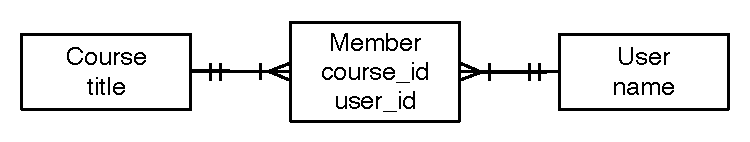
\includegraphics[keepaspectratio,alt={A Many to Many Connector Table},height=1.5in]{../images/many-to-many-verbose.eps}}
\caption{A Many to Many Connector Table\label{figm2mvrb}}
\end{figure}

\index{Through table} \index{Junction table} \index{Connector table}
\index{Join table} Instead of either of these approaches, we model a
many-to-many relationship using an additional table that we call a
``junction table'', ``through table'', ``connector table'', or ``join
table'' as shown in Figure \ref{figm2mvrb}. The purpose of this table is
to capture the \emph{connection} between \emph{a} course and \emph{a}
student.

In a sense the table sits between the \texttt{Course} and \texttt{User}
table and has a one-to-many relationship to both tables. By using an
intermediate table we break a many-to-many relationship into two
one-to-many relationships. Databases are very good at modeling and
processing one-to-many relationships.

An example \texttt{Member} table would be as follows:

\begin{Shaded}
\begin{Highlighting}[]
\KeywordTok{CREATE} \KeywordTok{TABLE} \FunctionTok{User}\NormalTok{ (}
    \KeywordTok{id}     \DataTypeTok{INTEGER} \KeywordTok{PRIMARY} \KeywordTok{KEY}\NormalTok{,}
\NormalTok{    name   TEXT }\KeywordTok{UNIQUE}
\NormalTok{);}

\KeywordTok{CREATE} \KeywordTok{TABLE}\NormalTok{ Course (}
    \KeywordTok{id}     \DataTypeTok{INTEGER} \KeywordTok{PRIMARY} \KeywordTok{KEY}\NormalTok{,}
\NormalTok{    title  TEXT }\KeywordTok{UNIQUE}
\NormalTok{);}

\KeywordTok{CREATE} \KeywordTok{TABLE} \KeywordTok{Member}\NormalTok{ (}
\NormalTok{    user\_id     }\DataTypeTok{INTEGER}\NormalTok{,}
\NormalTok{    course\_id   }\DataTypeTok{INTEGER}\NormalTok{,}
    \KeywordTok{PRIMARY} \KeywordTok{KEY}\NormalTok{ (user\_id, course\_id)}
\NormalTok{);}
\end{Highlighting}
\end{Shaded}

Following our naming convention, \texttt{Member.user\_id} and
\texttt{Member.course\_id} are foreign keys pointing at the
corresponding rows in the \texttt{User} and \texttt{Course} tables. Each
entry in the member table links a row in the \texttt{User} table to a
row in the \texttt{Course} table by going \emph{through} the
\texttt{Member} table.

\index{SQL!Constraint} We indicate that the \emph{combination} of
\texttt{course\_id} and \texttt{user\_id} is the \texttt{PRIMARY\ KEY}
for the \texttt{Member} table, also creating an uniqueness constraint
for a \texttt{course\_id} / \texttt{user\_id} combination.

Now lets say we need to insert a number of students into the rosters of
a number of courses. Lets assume the data comes to us in a
JSON-formatted file with records like this:

{\small
\begin{verbatim}
[
  [ "Charley", "si110"],
  [ "Mea", "si110"],
  [ "Hattie", "si110"],
  [ "Keziah", "si110"],
  [ "Rosa", "si106"],
  [ "Mea", "si106"],
  [ "Mairin", "si106"],
  [ "Zendel", "si106"],
  [ "Honie", "si106"],
  [ "Rosa", "si106"],
...
]
\end{verbatim}
}

\index{JSON!parse} We could write code as follows to read the JSON file
and insert the members of each course roster into the database using the
following code:

\begin{Shaded}
\begin{Highlighting}[]
\ImportTok{import}\NormalTok{ json}
\ImportTok{import}\NormalTok{ sqlite3}

\NormalTok{conn }\OperatorTok{=}\NormalTok{ sqlite3.}\ExtensionTok{connect}\NormalTok{(}\StringTok{\textquotesingle{}rosterdb.sqlite\textquotesingle{}}\NormalTok{)}
\NormalTok{cur }\OperatorTok{=}\NormalTok{ conn.cursor()}

\NormalTok{str\_data }\OperatorTok{=} \BuiltInTok{open}\NormalTok{(}\StringTok{\textquotesingle{}roster\_data\_sample.json\textquotesingle{}}\NormalTok{).read()}
\NormalTok{json\_data }\OperatorTok{=}\NormalTok{ json.loads(str\_data)}

\ControlFlowTok{for}\NormalTok{ entry }\KeywordTok{in}\NormalTok{ json\_data:}

\NormalTok{    name }\OperatorTok{=}\NormalTok{ entry[}\DecValTok{0}\NormalTok{]}
\NormalTok{    title }\OperatorTok{=}\NormalTok{ entry[}\DecValTok{1}\NormalTok{]}

    \BuiltInTok{print}\NormalTok{((name, title))}

\NormalTok{    cur.execute(}\StringTok{\textquotesingle{}\textquotesingle{}\textquotesingle{}INSERT OR IGNORE INTO User (name)}
\StringTok{        VALUES ( ? )\textquotesingle{}\textquotesingle{}\textquotesingle{}}\NormalTok{, ( name, ) )}
\NormalTok{    cur.execute(}\StringTok{\textquotesingle{}SELECT id FROM User WHERE name = ? \textquotesingle{}}\NormalTok{, (name, ))}
\NormalTok{    user\_id }\OperatorTok{=}\NormalTok{ cur.fetchone()[}\DecValTok{0}\NormalTok{]}

\NormalTok{    cur.execute(}\StringTok{\textquotesingle{}\textquotesingle{}\textquotesingle{}INSERT OR IGNORE INTO Course (title)}
\StringTok{        VALUES ( ? )\textquotesingle{}\textquotesingle{}\textquotesingle{}}\NormalTok{, ( title, ) )}
\NormalTok{    cur.execute(}\StringTok{\textquotesingle{}SELECT id FROM Course WHERE title = ? \textquotesingle{}}\NormalTok{, (title, ))}
\NormalTok{    course\_id }\OperatorTok{=}\NormalTok{ cur.fetchone()[}\DecValTok{0}\NormalTok{]}

\NormalTok{    cur.execute(}\StringTok{\textquotesingle{}\textquotesingle{}\textquotesingle{}INSERT OR REPLACE INTO Member}
\StringTok{        (user\_id, course\_id) VALUES ( ?, ? )\textquotesingle{}\textquotesingle{}\textquotesingle{}}\NormalTok{,}
\NormalTok{        ( user\_id, course\_id ) )}

\NormalTok{    conn.commit()}
\end{Highlighting}
\end{Shaded}

Like in a previous example, we first make sure that we have an entry in
the \texttt{User} table and know the primary key of the entry as well as
an entry in the \texttt{Course} table and know its primary key. We use
the `INSERT OR IGNORE' and `SELECT' pattern so our code works regardless
of whether the record is in the table or not.

Our insert into the \texttt{Member} table is simply inserting the two
integers as a new or existing row depending on the constraint to make
sure we do not end up with duplicate entries in the \texttt{Member}
table for a particular \texttt{user\_id} / \texttt{course\_id}
combination.

\index{SQL!JOIN} To reconstruct our data across all three tables, we
again use \texttt{JOIN} / \texttt{ON} to construct a \texttt{SELECT}
query;

{\small
\begin{verbatim}
sqlite> SELECT * FROM Course
   ...> JOIN Member ON Course.id = Member.course_id
   ...> JOIN User ON Member.user_id = User.id;
+----+-------+---------+-----------+----+---------+
| id | title | user_id | course_id | id |  name   |
+----+-------+---------+-----------+----+---------+
| 1  | si110 | 1       | 1         | 1  | Charley |
| 1  | si110 | 2       | 1         | 2  | Mea     |
| 1  | si110 | 3       | 1         | 3  | Hattie  |
| 1  | si110 | 4       | 1         | 4  | Lyena   |
| 1  | si110 | 5       | 1         | 5  | Keziah  |
| 1  | si110 | 6       | 1         | 6  | Ellyce  |
| 1  | si110 | 7       | 1         | 7  | Thalia  |
| 1  | si110 | 8       | 1         | 8  | Meabh   |
| 2  | si106 | 2       | 2         | 2  | Mea     |
| 2  | si106 | 10      | 2         | 10 | Mairin  |
| 2  | si106 | 11      | 2         | 11 | Zendel  |
| 2  | si106 | 12      | 2         | 12 | Honie   |
| 2  | si106 | 9       | 2         | 9  | Rosa    |
+----+-------+---------+-----------+----+---------+
sqlite>
\end{verbatim}
}

You can see the three tables from left to right - \texttt{Course},
\texttt{Member}, and \texttt{User} and you can see the connections
between the primary keys and foreign keys in each row of output.

\section{Modeling data at the many-to-many
connection}\label{modeling-data-at-the-many-to-many-connection}

While we have presented the ``join table'' as having two foreign keys
making a connection between rows in two tables, this is the simplest
form of a join table. It is quite common to want to add some data to the
connection itself.

Continuing with our example of users, courses, and rosters to model a
simple learning management system, we will also need to understand the
\emph{role} that each user is assigned in each course.

If we first try to solve this by adding an ``instructor'' flag to the
\texttt{User} table, we will find that this does not work because a user
can be a instructor in one course and a student in another course. If we
add an \texttt{instructor\_id} to the \texttt{Course} table it will not
work because a course can have multiple instructors. And there is no
one-to-many hack that can deal with the fact that the number of roles
will expand into roles like Teaching Assistant or Parent.

But if we simply add a \texttt{role} column to the \texttt{Member} table
- we can represent a wide range of roles, role combinations, etc.

Lets change our member table as follows:

\begin{Shaded}
\begin{Highlighting}[]
\KeywordTok{DROP} \KeywordTok{TABLE} \KeywordTok{Member}\NormalTok{;}

\KeywordTok{CREATE} \KeywordTok{TABLE} \KeywordTok{Member}\NormalTok{ (}
\NormalTok{    user\_id     }\DataTypeTok{INTEGER}\NormalTok{,}
\NormalTok{    course\_id   }\DataTypeTok{INTEGER}\NormalTok{,}
    \KeywordTok{role}        \DataTypeTok{INTEGER}\NormalTok{,}
    \KeywordTok{PRIMARY} \KeywordTok{KEY}\NormalTok{ (user\_id, course\_id)}
\NormalTok{);}
\end{Highlighting}
\end{Shaded}

Para sa simplicity, magde-decide tayo na zero sa role ay
nangangahulugang ``student'' at isa sa \texttt{role} ay nangangahulugang
instructor. Ipagpalagay natin na ang JSON data natin ay na-augment ng
role tulad ng sumusunod:

{\small
\begin{verbatim}
[
  [ "Charley", "si110", 1],
  [ "Mea", "si110", 0],
  [ "Hattie", "si110", 0],
  [ "Keziah", "si110", 0],
  [ "Rosa", "si106", 0],
  [ "Mea", "si106", 1],
  [ "Mairin", "si106", 0],
  [ "Zendel", "si106", 0],
  [ "Honie", "si106", 0],
  [ "Rosa", "si106", 0],
...
]
\end{verbatim}
}

Maaari nating baguhin ang program na \texttt{roster.py} sa itaas para
isama ang role tulad ng sumusunod:

\begin{Shaded}
\begin{Highlighting}[]
\ControlFlowTok{for}\NormalTok{ entry }\KeywordTok{in}\NormalTok{ json\_data:}

\NormalTok{    name }\OperatorTok{=}\NormalTok{ entry[}\DecValTok{0}\NormalTok{]}
\NormalTok{    title }\OperatorTok{=}\NormalTok{ entry[}\DecValTok{1}\NormalTok{]}
\NormalTok{    role }\OperatorTok{=}\NormalTok{ entry[}\DecValTok{2}\NormalTok{]}

\NormalTok{    ...}

\NormalTok{    cur.execute(}\StringTok{\textquotesingle{}\textquotesingle{}\textquotesingle{}INSERT OR REPLACE INTO Member}
\StringTok{        (user\_id, course\_id, role) VALUES ( ?, ?, ? )\textquotesingle{}\textquotesingle{}\textquotesingle{}}\NormalTok{,}
\NormalTok{        ( user\_id, course\_id, role ) )}
\end{Highlighting}
\end{Shaded}

Sa tunay na system, malamang gagawa tayo ng \texttt{Role} table at gawin
ang \texttt{role} column sa \texttt{Member} na foreign key sa Role table
tulad ng sumusunod:

\begin{Shaded}
\begin{Highlighting}[]
\KeywordTok{DROP} \KeywordTok{TABLE} \KeywordTok{Member}\NormalTok{;}

\KeywordTok{CREATE} \KeywordTok{TABLE} \KeywordTok{Member}\NormalTok{ (}
\NormalTok{    user\_id     }\DataTypeTok{INTEGER}\NormalTok{,}
\NormalTok{    course\_id   }\DataTypeTok{INTEGER}\NormalTok{,}
\NormalTok{    role\_id     }\DataTypeTok{INTEGER}\NormalTok{,}
    \KeywordTok{PRIMARY} \KeywordTok{KEY}\NormalTok{ (user\_id, course\_id, role\_id)}
\NormalTok{);}

\KeywordTok{CREATE} \KeywordTok{TABLE} \KeywordTok{Role}\NormalTok{ (}
    \KeywordTok{id}          \DataTypeTok{INTEGER} \KeywordTok{PRIMARY} \KeywordTok{KEY}\NormalTok{,}
\NormalTok{    name        TEXT }\KeywordTok{UNIQUE}
\NormalTok{);}

\KeywordTok{INSERT} \KeywordTok{INTO} \KeywordTok{Role}\NormalTok{ (}\KeywordTok{id}\NormalTok{, name) }\KeywordTok{VALUES}\NormalTok{ (}\DecValTok{0}\NormalTok{, }\StringTok{\textquotesingle{}Student\textquotesingle{}}\NormalTok{);}
\KeywordTok{INSERT} \KeywordTok{INTO} \KeywordTok{Role}\NormalTok{ (}\KeywordTok{id}\NormalTok{, name) }\KeywordTok{VALUES}\NormalTok{ (}\DecValTok{1}\NormalTok{, }\StringTok{\textquotesingle{}Instructor\textquotesingle{}}\NormalTok{);}
\end{Highlighting}
\end{Shaded}

Notice that because we declared the \texttt{id} column in the
\texttt{Role} table as a \texttt{PRIMARY\ KEY}, we \emph{could} omit it
in the \texttt{INSERT} statement. But we can also choose the \texttt{id}
value as long as the value is not already in the \texttt{id} column and
does not violate the implied \texttt{UNIQUE} constaint on primary keys.

\section{Summary}\label{summary-2}

This chapter has covered a lot of ground to give you an overview of the
basics of using a database in Python. It is more complicated to write
the code to use a database to store data than Python dictionaries or
flat files so there is little reason to use a database unless your
application truly needs the capabilities of a database. The situations
where a database can be quite useful are: (1) when your application
needs to make many small random updates within a large data set, (2)
when your data is so large it cannot fit in a dictionary and you need to
look up information repeatedly, or (3) when you have a long-running
process that you want to be able to stop and restart and retain the data
from one run to the next.

You can build a simple database with a single table to suit many
application needs, but most problems will require several tables and
links/relationships between rows in different tables. When you start
making links between tables, it is important to do some thoughtful
design and follow the rules of database normalization to make the best
use of the database's capabilities. Since the primary motivation for
using a database is that you have a large amount of data to deal with,
it is important to model your data efficiently so your programs run as
fast as possible.

\section{Debugging}\label{debugging-11}

Ang isang karaniwang pattern kapag gumagawa ka ng Python program para
kumonekta sa SQLite database ay patakbuhin ang Python program at suriin
ang results gamit ang Database Browser for SQLite. Ang browser ay
nagpapahintulot sa iyo na mabilis na suriin kung gumagana nang maayos
ang program mo.

Dapat kang maging maingat dahil ang SQLite ay nag-aalaga para pigilan
ang dalawang programs na baguhin ang parehong data nang sabay.
Halimbawa, kung bubuksan mo ang database sa browser at gumawa ng
pagbabago sa database at hindi pa na-press ang ``save'' button sa
browser, ang browser ay ``naglo-lock'' ng database file at pumipigil sa
anumang iba pang program na ma-access ang file. Sa partikular, ang
Python program mo ay hindi makaka-access sa file kung naka-lock ito.

Kaya ang solusyon ay siguraduhing isara ang database browser o gamitin
ang \emph{File} menu para isara ang database sa browser bago subukang
ma-access ang database mula sa Python para maiwasan ang problema ng
Python code mo na mabigo dahil naka-lock ang database.

\section{Glossary}\label{glossary-14}

\begin{description}
\tightlist
\item[attribute]
Isa sa mga values sa loob ng tuple. Mas karaniwang tinatawag na
``column'' o ``field''. \index{attribute}
\item[constraint]
Kapag sinasabi natin sa database na ipatupad ang rule sa field o row sa
table. Ang karaniwang constraint ay pagpilit na hindi maaaring magkaroon
ng duplicate values sa partikular na field (i.e., lahat ng values ay
dapat unique). \index{constraint}
\item[cursor]
Ang cursor ay nagpapahintulot sa iyo na mag-execute ng SQL commands sa
database at kumuha ng data mula sa database. Ang cursor ay katulad ng
socket o file handle para sa network connections at files, ayon sa
pagkakabanggit. \index{cursor}
\item[database browser]
Piraso ng software na nagpapahintulot sa iyo na direktang kumonekta sa
database at manipulahin ang database nang direkta nang hindi sumusulat
ng program. \index{database browser}
\item[foreign key]
Numeric key na tumuturo sa primary key ng row sa iba pang table. Ang
foreign keys ay nagtatatag ng relationships sa pagitan ng rows na
naka-store sa iba't ibang tables. \index{foreign key}
\item[index]
Karagdagang data na nagma-maintain ang database software bilang rows at
nag-i-insert sa table para gawing napakabilis ang lookups. \index{index}
\index{}
\item[logical key]
Key na ginagamit ng ``outside world'' para maghanap ng partikular na
row. Para sa halimbawa sa table ng user accounts, ang email address ng
tao ay maaaring maging magandang kandidato bilang logical key para sa
data ng user. \index{logical key}
\item[normalization]
Pagde-design ng data model para walang data na na-replicate. Nag-i-store
tayo ng bawat item ng data sa isang lugar sa database at nagre-reference
dito sa ibang lugar gamit ang foreign key. \index{normalization}
\index{database normalization}
\item[primary key]
Numeric key na na-a-assign sa bawat row na ginagamit para tumukoy sa
isang row sa table mula sa iba pang table. Kadalasan ang database ay
naka-configure para awtomatikong mag-assign ng primary keys habang
na-i-insert ang rows. \index{primary key}
\item[relation]
Area sa loob ng database na naglalaman ng tuples at attributes. Mas
karaniwang tinatawag na ``table''. \index{relation}
\item[tuple]
Isang entry sa database table na set ng attributes. Mas karaniwang
tinatawag na ``row''.
\end{description}

\index{tuple}

\chapter{Visualizing data}\label{visualizing-data}

Hanggang ngayon natututo tayo ng Python language at pagkatapos natututo
kung paano gamitin ang Python, network, at databases para manipulahin
ang data.

Sa chapter na ito, titingnan natin ang tatlong kumpletong applications
na pinagsasama ang lahat ng mga bagay na ito para pamahalaan at
i-visualize ang data. Maaari mong gamitin ang mga applications na ito
bilang sample code para matulungan kang magsimula sa pagsolusyon ng
real-world problem.

Ang bawat isa sa applications ay ZIP file na maaari mong i-download at
i-extract sa computer mo at i-execute.

\section{Building a OpenStreetMap from geocoded
data}\label{building-a-openstreetmap-from-geocoded-data}

\index{Google!map} \index{OpenStreetMap} \index{Visualization!map}

Sa project na ito, gumagamit tayo ng OpenStreetMap geocoding API para
linisin ang ilang user-entered geographic locations ng university names
at pagkatapos ilagay ang data sa aktwal na OpenStreetMap.

\begin{figure}
\centering
\pandocbounded{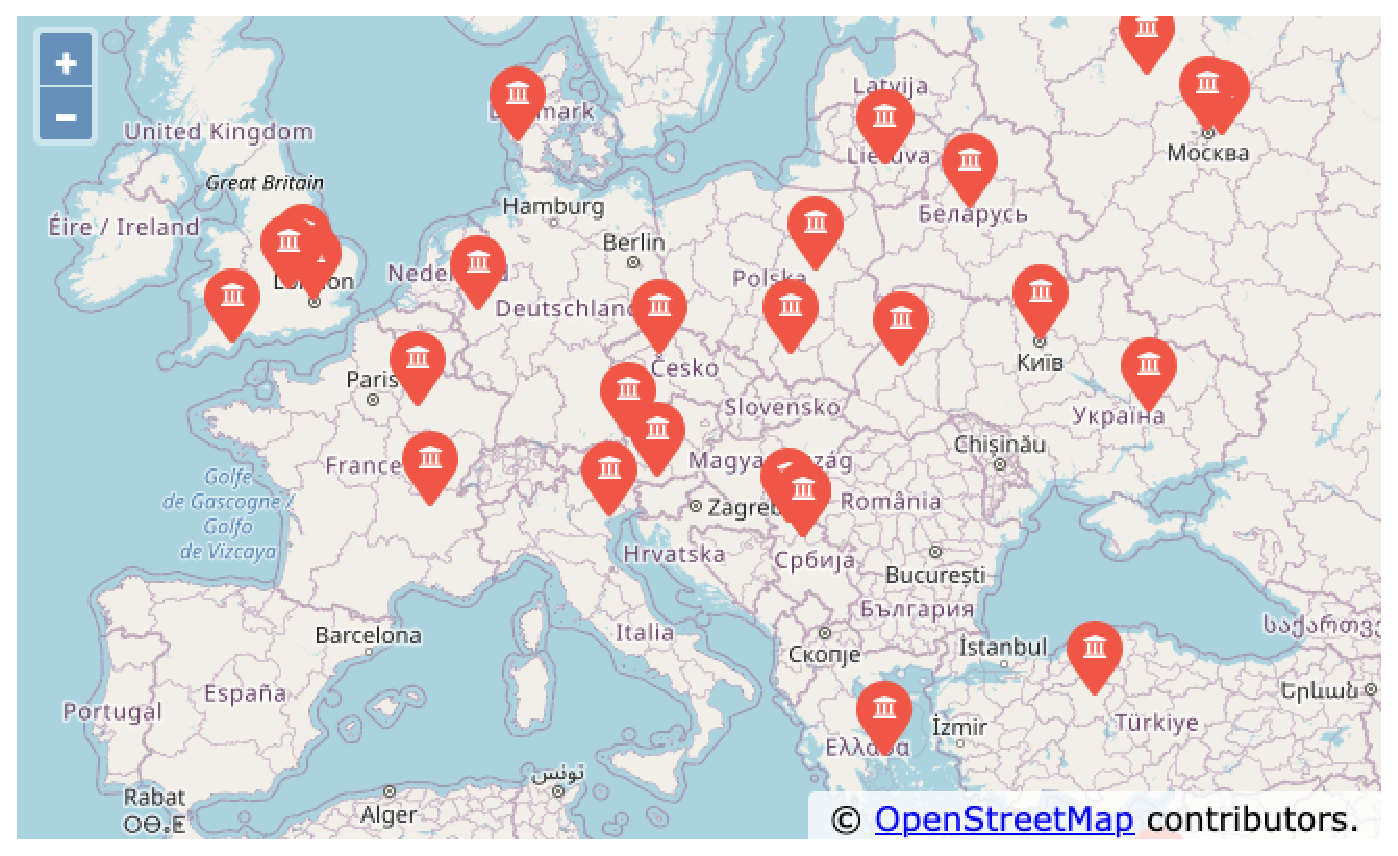
\includegraphics[keepaspectratio,alt={An OpenStreetMap}]{../images/openstreet-map.eps}}
\caption{An OpenStreetMap}
\end{figure}

Para magsimula, i-download ang application mula sa:

\href{http://www.py4e.com/code3/opengeo.zip}{www.py4e.com/code3/opengeo.zip}

Ang unang problema na solusyonan ay ang mga geocoding APIs na ito ay
rate-limited sa tiyak na bilang ng requests bawat araw. Kung mayroon
kang maraming data, maaaring kailangan mong huminto at muling simulan
ang lookup process nang ilang beses. Kaya hinahati natin ang problema sa
dalawang phases.

\index{cache}

Sa unang phase kinukuha natin ang input ``survey'' data natin sa file
\emph{where.data} at binabasa ito isang linya sa isang pagkakataon, at
kumukuha ng geocoded information mula sa Google at nag-i-store nito sa
database \emph{geodata.sqlite}. Bago gamitin ang geocoding API para sa
bawat user-entered location, simpleng sinusuri natin kung mayroon na
tayong data para sa partikular na linya ng input. Ang database ay
gumagana bilang local ``cache'' ng geocoding data natin para siguraduhin
na hindi tayo kailanman hihingi sa Google ng parehong data nang dalawang
beses.

Maaari mong muling simulan ang proseso anumang oras sa pamamagitan ng
pagtanggal ng file \emph{geodata.sqlite}.

Patakbuhin ang \emph{geoload.py} program. Ang program na ito ay
magbabasa ng input lines sa \emph{where.data} at para sa bawat linya
susuriin kung nasa database na ito. Kung wala tayong data para sa
location, tatawagin nito ang geocoding API para kunin ang data at
i-store ito sa database.

Narito ang sample run pagkatapos mayroon nang ilang data sa database:

{\small
\begin{verbatim}
Found in database AGH University of Science and Technology

Found in database Academy of Fine Arts Warsaw Poland

Found in database American University in Cairo

Found in database Arizona State University

Found in database Athens Information Technology

Retrieving https://py4e-data.dr-chuck.net/
   opengeo?q=BITS+Pilani
Retrieved 794 characters {"type":"FeatureColl

Retrieving https://py4e-data.dr-chuck.net/
   opengeo?q=Babcock+University
Retrieved 760 characters {"type":"FeatureColl

Retrieving https://py4e-data.dr-chuck.net/
   opengeo?q=Banaras+Hindu+University
Retrieved 866 characters {"type":"FeatureColl
...
\end{verbatim}
}

Ang unang limang locations ay nasa database na at kaya sila ay na-skip.
Ang program ay nag-scan hanggang sa punto kung saan nakakahanap ito ng
bagong locations at nagsisimulang kunin ang mga ito.

Ang \emph{geoload.py} program ay maaaring itigil anumang oras, at
mayroong counter na maaari mong gamitin para limitahan ang bilang ng
tawag sa geocoding API para sa bawat run. Dahil ang \emph{where.data} ay
may ilang daang data items lang, hindi ka dapat makakaranas ng daily
rate limit, pero kung mayroon kang mas maraming data maaaring kailangan
ng ilang runs sa loob ng ilang araw para magkaroon ang database mo ng
lahat ng geocoded data para sa input mo.

Kapag mayroon ka nang ilang data na na-load sa \emph{geodata.sqlite},
maaari mong i-visualize ang data gamit ang \emph{geodump.py} program.
Ang program na ito ay nagbabasa ng database at sumusulat ng file
\emph{where.js} na may location, latitude, at longitude sa form ng
executable JavaScript code.

Ang run ng \emph{geodump.py} program ay ganito:

{\small
\begin{verbatim}
AGH University of Science and Technology, Czarnowiejska,
Czarna Wie's, Krowodrza, Krak'ow, Lesser Poland
Voivodeship, 31-126, Poland 50.0657 19.91895

Academy of Fine Arts, Krakowskie Przedmie'scie,
Northern 'Sr'odmie'scie, 'Sr'odmie'scie, Warsaw, Masovian
Voivodeship, 00-046, Poland 52.239 21.0155
...
260 lines were written to where.js
Open the where.html file in a web browser to view the data.
\end{verbatim}
}

Ang file na \emph{where.html} ay binubuo ng HTML at JavaScript para
i-visualize ang Google map. Binabasa nito ang pinakabagong data sa
\emph{where.js} para makuha ang data na i-visualize. Narito ang format
ng file na \emph{where.js}:

\begin{Shaded}
\begin{Highlighting}[]
\NormalTok{myData }\OperatorTok{=}\NormalTok{ [}
\NormalTok{[}\FloatTok{50.0657}\OperatorTok{,}\FloatTok{19.91895}\OperatorTok{,}
\StringTok{\textquotesingle{}AGH University of Science and Technology, Czarnowiejska,}
\NormalTok{Czarna Wie}\StringTok{\textquotesingle{}s, Krowodrza, Krak\textquotesingle{}}\NormalTok{ow}\OperatorTok{,}\NormalTok{ Lesser Poland}
\NormalTok{Voivodeship}\OperatorTok{,} \DecValTok{31}\OperatorTok{{-}}\DecValTok{126}\OperatorTok{,}\NormalTok{ Poland }\StringTok{\textquotesingle{}],}
\NormalTok{[}\FloatTok{52.239}\OperatorTok{,}\FloatTok{21.0155}\OperatorTok{,}
\StringTok{\textquotesingle{}Academy of Fine Arts, Krakowskie Przedmie\textquotesingle{}}\NormalTok{sciee}\OperatorTok{,}
\StringTok{\textquotesingle{}Sr\textquotesingle{}}\NormalTok{odmie}\StringTok{\textquotesingle{}scie P\textquotesingle{}}\NormalTok{olnocne}\OperatorTok{,} \StringTok{\textquotesingle{}Sr\textquotesingle{}}\NormalTok{odmie}\StringTok{\textquotesingle{}scie, Warsaw,}
\NormalTok{Masovian Voivodeship}\OperatorTok{,} \DecValTok{00}\OperatorTok{{-}}\BaseNTok{046}\OperatorTok{,}\NormalTok{ Poland}\StringTok{\textquotesingle{}],}
   \OperatorTok{...}
\NormalTok{]}\OperatorTok{;}
\end{Highlighting}
\end{Shaded}

Ito ay JavaScript variable na naglalaman ng list ng lists. Ang syntax
para sa JavaScript list constants ay napakatulad sa Python, kaya ang
syntax ay dapat pamilyar sa iyo.

Simpleng buksan ang \emph{where.html} sa browser para makita ang
locations. Maaari mong i-hover sa bawat map pin para hanapin ang
location na ibinalik ng geocoding API para sa user-entered input. Kung
hindi mo makita ang anumang data kapag binubuksan mo ang file na
\emph{where.html}, maaaring gusto mong suriin ang JavaScript o developer
console para sa browser mo.

\section{Visualizing networks and
interconnections}\label{visualizing-networks-and-interconnections}

\index{Google!page rank} \index{Visualization!networks}
\index{Visualization!page rank}

Sa application na ito, gagawa tayo ng ilang functions ng search engine.
Una tayong mag-spider ng maliit na subset ng web at magpatakbo ng
simplified version ng Google page rank algorithm para matukoy kung alin
ang pages na pinakamataas ang connectivity, at pagkatapos i-visualize
ang page rank at connectivity ng maliit na sulok natin ng web. Gagamitin
natin ang D3 JavaScript visualization library \url{http://d3js.org/}
para gumawa ng visualization output.

Maaari mong i-download at i-extract ang application na ito mula sa:

\href{http://www.py4e.com/code3/pagerank.zip}{www.py4e.com/code3/pagerank.zip}

\begin{figure}
\centering
\pandocbounded{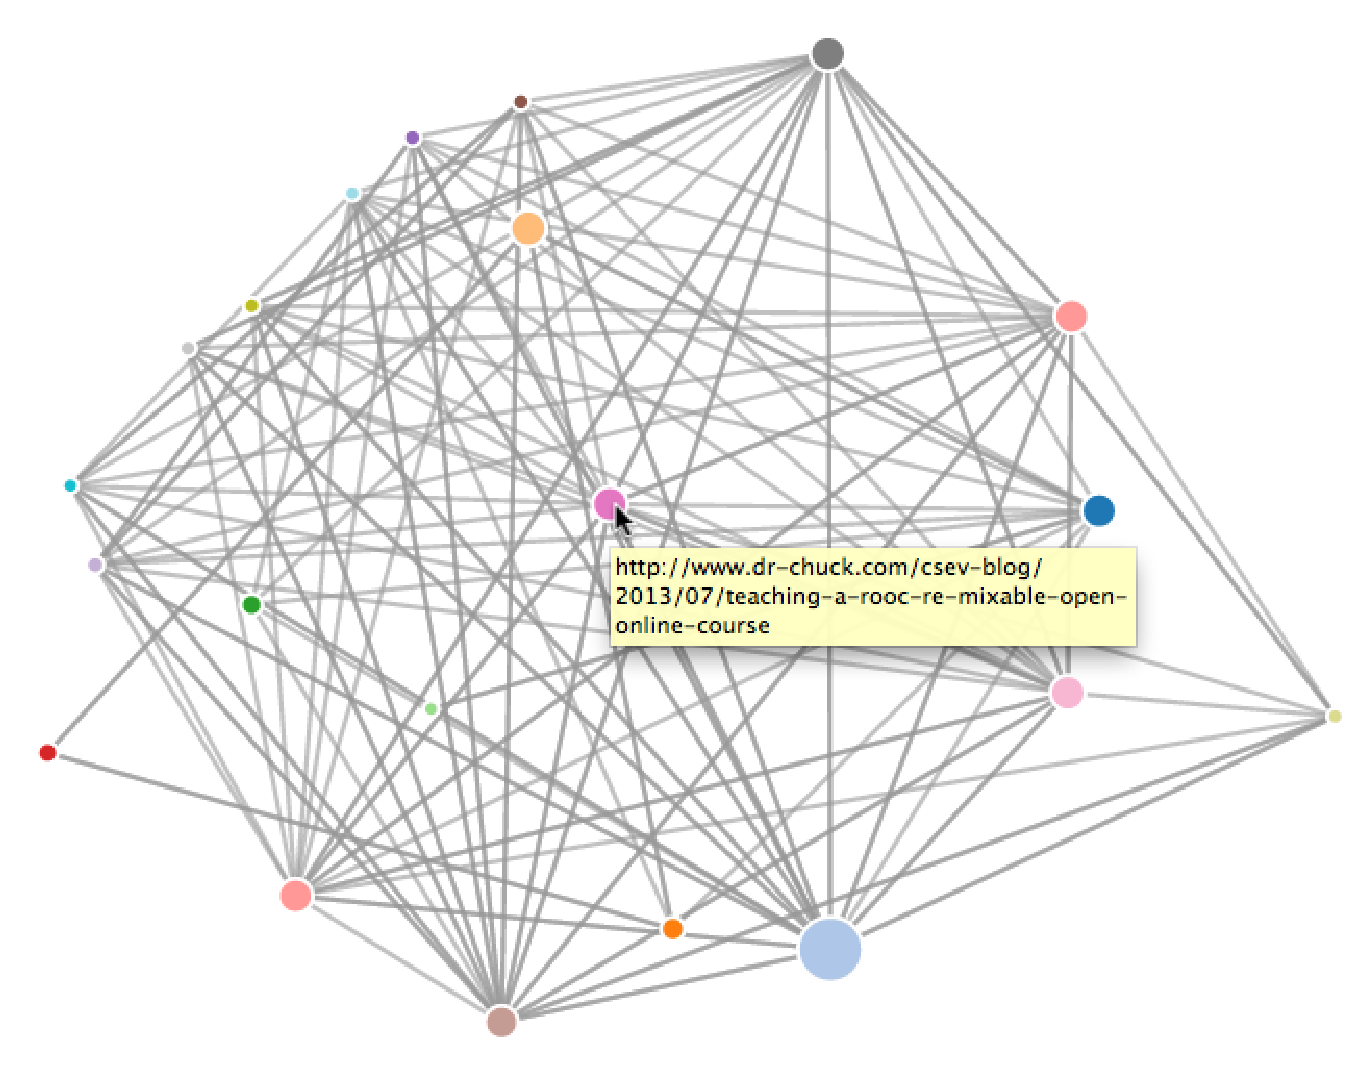
\includegraphics[keepaspectratio,alt={A Page Ranking},height=3.5in]{../images/pagerank.eps}}
\caption{A Page Ranking}
\end{figure}

Ang unang program (\emph{spider.py}) ay nag-crawl ng web site at
kumukuha ng serye ng pages sa database (\emph{spider.sqlite}), na
nagre-record ng links sa pagitan ng pages. Maaari mong muling simulan
ang proseso anumang oras sa pamamagitan ng pagtanggal ng file na
\emph{spider.sqlite} at muling pagpatakbo ng \emph{spider.py}.

{\small
\begin{verbatim}
Enter web url or enter: http://www.dr-chuck.com/
['http://www.dr-chuck.com']
How many pages:2
1 http://www.dr-chuck.com/ 12
2 http://www.dr-chuck.com/csev-blog/ 57
How many pages:
\end{verbatim}
}

Sa sample run na ito, sinabi natin sa kanya na i-crawl ang website at
kunin ang dalawang pages. Kung muling patakbuhin mo ang program at
sabihin sa kanya na i-crawl ang mas maraming pages, hindi ito
magre-crawl ng anumang pages na nasa database na. Sa pag-restart
pumupunta ito sa random na non-crawled page at nagsisimula doon. Kaya
ang bawat sunud-sunod na run ng \emph{spider.py} ay additive.

{\small
\begin{verbatim}
Enter web url or enter: http://www.dr-chuck.com/
['http://www.dr-chuck.com']
How many pages:3
3 http://www.dr-chuck.com/csev-blog 57
4 http://www.dr-chuck.com/dr-chuck/resume/speaking.htm 1
5 http://www.dr-chuck.com/dr-chuck/resume/index.htm 13
How many pages:
\end{verbatim}
}

Maaari kang magkaroon ng maraming starting points sa parehong
database-sa loob ng program, ang mga ito ay tinatawag na ``webs''. Ang
spider ay pumipili nang random sa lahat ng non-visited links sa lahat ng
webs bilang susunod na page na i-spider.

Kung gusto mong i-dump ang contents ng file na \emph{spider.sqlite},
maaari mong patakbuhin ang \emph{spdump.py} tulad ng sumusunod:

{\small
\begin{verbatim}
(5, None, 1.0, 3, 'http://www.dr-chuck.com/csev-blog')
(3, None, 1.0, 4, 'http://www.dr-chuck.com/dr-chuck/resume/speaking.htm')
(1, None, 1.0, 2, 'http://www.dr-chuck.com/csev-blog/')
(1, None, 1.0, 5, 'http://www.dr-chuck.com/dr-chuck/resume/index.htm')
4 rows.
\end{verbatim}
}

Ipinapakita nito ang bilang ng incoming links, ang lumang page rank, ang
bagong page rank, ang id ng page, at ang url ng page. Ang program na
\emph{spdump.py} ay nagpapakita lang ng pages na may hindi bababa sa
isang incoming link sa kanila.

Kapag mayroon ka nang ilang pages sa database, maaari mong patakbuhin
ang page rank sa pages gamit ang program na \emph{sprank.py}. Simpleng
sinasabi mo lang sa kanya kung ilang page rank iterations ang
patakbuhin.

{\small
\begin{verbatim}
How many iterations:2
1 0.546848992536
2 0.226714939664
[(1, 0.559), (2, 0.659), (3, 0.985), (4, 2.135), (5, 0.659)]
\end{verbatim}
}

Maaari mong i-dump ang database ulit para makita na na-update na ang
page rank:

{\small
\begin{verbatim}
(5, 1.0, 0.985, 3, 'http://www.dr-chuck.com/csev-blog')
(3, 1.0, 2.135, 4, 'http://www.dr-chuck.com/dr-chuck/resume/speaking.htm')
(1, 1.0, 0.659, 2, 'http://www.dr-chuck.com/csev-blog/')
(1, 1.0, 0.659, 5, 'http://www.dr-chuck.com/dr-chuck/resume/index.htm')
4 rows.
\end{verbatim}
}

Maaari mong patakbuhin ang \emph{sprank.py} nang maraming beses hangga't
gusto mo at ito ay simpleng magre-refine ng page rank sa bawat
pagkakataon na patakbuhin mo ito. Maaari mo ring patakbuhin ang
\emph{sprank.py} nang ilang beses at pagkatapos mag-spider ng ilang
higit pang pages gamit ang \emph{spider.py} at pagkatapos patakbuhin ang
\emph{sprank.py} para muling mag-converge ang page rank values. Ang
search engine ay karaniwang nagpapatakbo ng parehong crawling at ranking
programs sa lahat ng oras.

Kung gusto mong muling simulan ang page rank calculations nang hindi
muling nag-spider ng web pages, maaari mong gamitin ang
\emph{spreset.py} at pagkatapos muling simulan ang \emph{sprank.py}.

{\small
\begin{verbatim}
How many iterations:50
1 0.546848992536
2 0.226714939664
3 0.0659516187242
4 0.0244199333
5 0.0102096489546
6 0.00610244329379
...
42 0.000109076928206
43 9.91987599002e-05
44 9.02151706798e-05
45 8.20451504471e-05
46 7.46150183837e-05
47 6.7857770908e-05
48 6.17124694224e-05
49 5.61236959327e-05
50 5.10410499467e-05
[(512, 0.0296), (1, 12.79), (2, 28.93), (3, 6.808), (4, 13.46)]
\end{verbatim}
}

Para sa bawat iteration ng page rank algorithm nagpi-print ito ng
average change sa page rank per page. Ang network sa simula ay medyo
hindi balanse at kaya ang individual page rank values ay nagbabago nang
malaki sa pagitan ng iterations. Pero sa ilang maikling iterations, ang
page rank ay nagco-converge. Dapat mong patakbuhin ang \emph{sprank.py}
nang sapat na tagal para ang page rank values ay mag-converge.

Kung gusto mong i-visualize ang kasalukuyang top pages sa terms ng page
rank, patakbuhin ang \emph{spjson.py} para basahin ang database at
isulat ang data para sa pinakamataas na linked pages sa JSON format para
makita sa web browser.

{\small
\begin{verbatim}
Creating JSON output on spider.json...
How many nodes? 30
Open force.html in a browser to view the visualization
\end{verbatim}
}

Maaari mong tingnan ang data na ito sa pamamagitan ng pagbubukas ng file
na \emph{force.html} sa web browser mo. Ipinapakita nito ang automatic
layout ng nodes at links. Maaari mong i-click at i-drag ang anumang node
at maaari mo ring i-double-click ang node para hanapin ang URL na
kinakatawan ng node.

Kung muling patakbuhin mo ang iba pang utilities, muling patakbuhin ang
\emph{spjson.py} at pindutin ang refresh sa browser para makuha ang
bagong data mula sa \emph{spider.json}.

\section{Visualizing mail data}\label{visualizing-mail-data}

Hanggang sa puntong ito sa libro, naging pamilyar ka na sa aming
\emph{mbox-short.txt} at \emph{mbox.txt} data files. Ngayon panahon na
para dalhin ang analysis natin ng email data sa susunod na level.

Sa totoong mundo, minsan kailangan mong kunin ang mail data mula sa
servers. Maaaring tumagal ito ng ilang panahon at ang data ay maaaring
hindi consistent, puno ng error, at nangangailangan ng maraming cleanup
o adjustment. Sa section na ito, nagtatrabaho tayo sa application na
pinakakumplikado hanggang ngayon at kumukuha ng halos gigabyte ng data
at i-visualize ito.

\begin{figure}
\centering
\pandocbounded{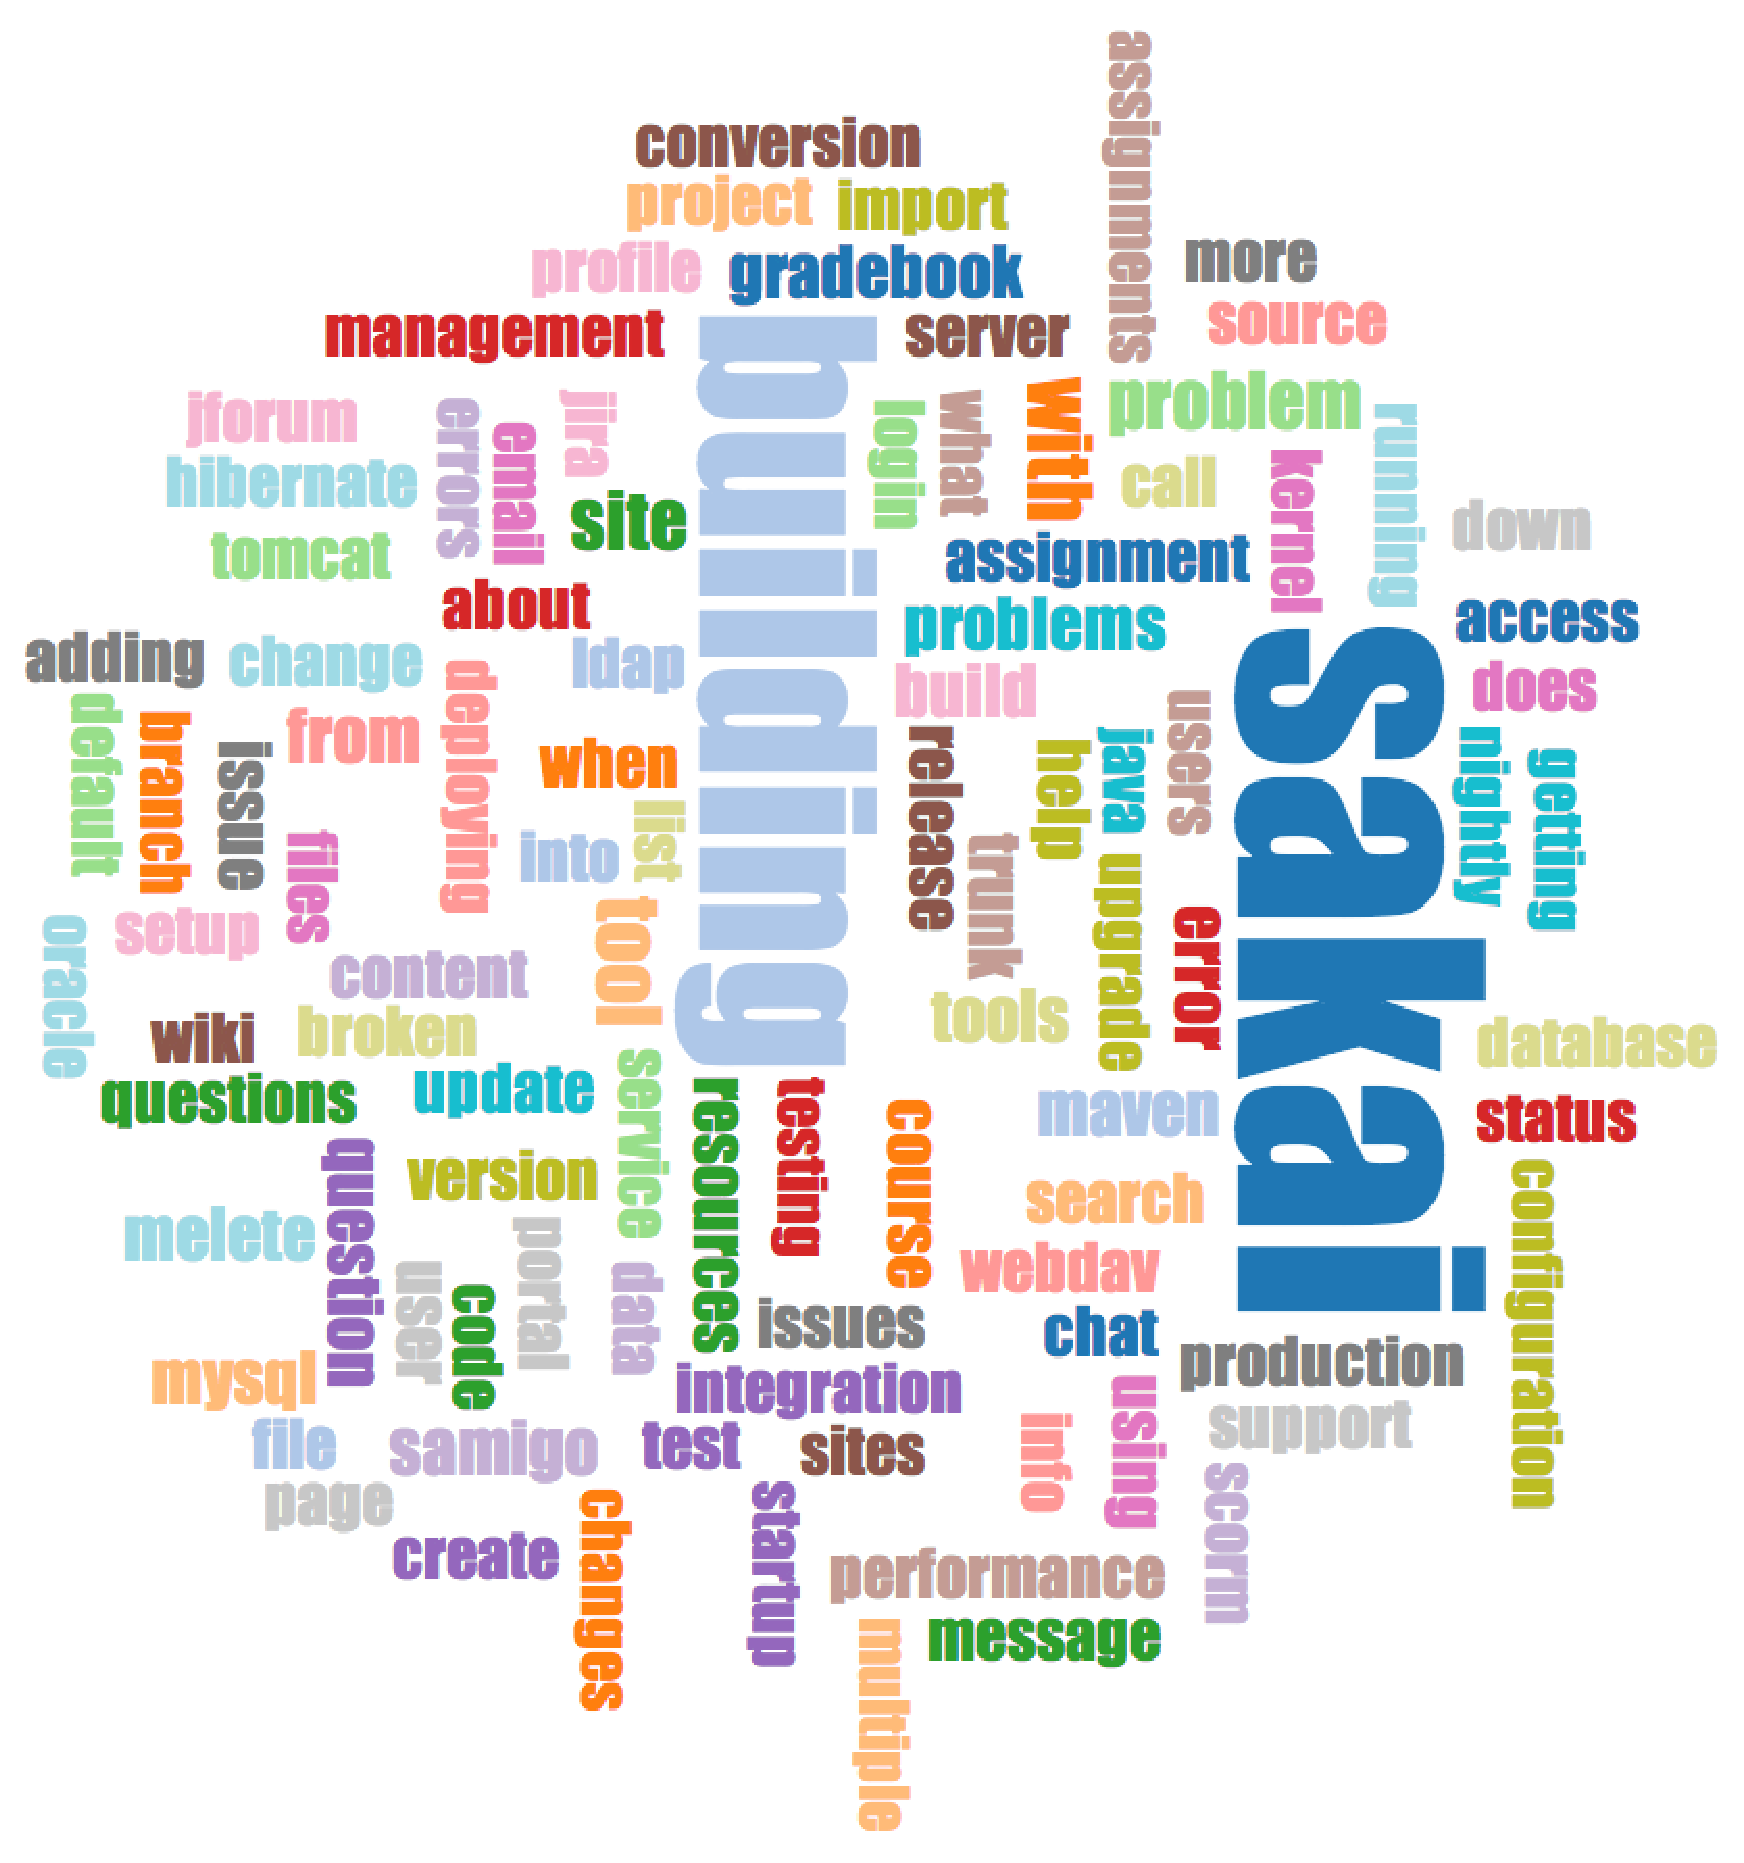
\includegraphics[keepaspectratio,alt={A Word Cloud from the Sakai Developer List},height=3.5in]{../images/wordcloud.eps}}
\caption{A Word Cloud from the Sakai Developer List}
\end{figure}

Maaari mong i-download ang application na ito mula sa:

\url{https://www.py4e.com/code3/gmane.zip}

Gagamitin natin ang data mula sa libreng email list archiving service na
tinatawag na \emph{gmane} - ang service ay na-shut down na at para sa
layunin ng course na ito, ang partial archive ay na-maintain sa
\url{http://mbox.dr-chuck.net}. Ang gmane service ay napakapopular sa
open source projects dahil nagbibigay ito ng magandang searchable
archive ng kanilang email activity.

\url{http://mbox.dr-chuck.net/export.php}

Kapag ang Sakai email data ay na-spider gamit ang software na ito,
gumawa ito ng halos Gigabyte ng data at tumagal ng ilang runs sa loob ng
ilang araw. Ang file na \emph{README.txt} sa ZIP sa itaas ay maaaring
may instructions tungkol sa kung paano mo maaaring i-download ang
pre-spidered copy ng file na \emph{content.sqlite} para sa karamihan ng
Sakai email corpus para hindi mo kailangang mag-spider ng limang araw
lang para patakbuhin ang programs. Kung i-download mo ang pre-spidered
content, dapat mo pa ring patakbuhin ang spidering process para
makahabol sa mas bagong messages.

Ang unang hakbang ay i-spider ang repository. Ang base URL ay hard-coded
sa \emph{gmane.py} at hard-coded sa Sakai developer list. Maaari mong
i-spider ang iba pang repository sa pamamagitan ng pagbabago ng base url
na iyon. Siguraduhing tanggalin ang file na \emph{content.sqlite} kung
magpapalit ka ng base url.

Ang file na \emph{gmane.py} ay gumagana bilang responsible caching
spider sa diwa na mabagal itong tumatakbo at kumukuha ng isang mail
message bawat segundo para maiwasan ang ma-throttle. Nag-i-store ito ng
lahat ng data nito sa database at maaaring ma-interrupt at muling
simulan nang kasing dami ng kailangan. Maaari itong tumagal ng maraming
oras para kunin ang lahat ng data. Kaya maaaring kailangan mong muling
simulan nang ilang beses.

Narito ang run ng \emph{gmane.py} na kumukuha ng huling limang messages
ng Sakai developer list:

{\small
\begin{verbatim}
How many messages:10
http://mbox.dr-chuck.net/sakai.devel/51410/51411 9460
    nealcaidin@sakaifoundation.org 2013-04-05 re: [building ...
http://mbox.dr-chuck.net/sakai.devel/51411/51412 3379
    samuelgutierrezjimenez@gmail.com 2013-04-06 re: [building ...
http://mbox.dr-chuck.net/sakai.devel/51412/51413 9903
    da1@vt.edu 2013-04-05 [building sakai] melete 2.9 oracle ...
http://mbox.dr-chuck.net/sakai.devel/51413/51414 349265
    m.shedid@elraed-it.com 2013-04-07 [building sakai] ...
http://mbox.dr-chuck.net/sakai.devel/51414/51415 3481
    samuelgutierrezjimenez@gmail.com 2013-04-07 re: ...
http://mbox.dr-chuck.net/sakai.devel/51415/51416 0

Does not start with From
\end{verbatim}
}

Ang program ay nag-scan ng \emph{content.sqlite} mula sa isa hanggang sa
unang message number na hindi pa na-spider at nagsisimulang mag-spider
sa message na iyon. Nagpapatuloy ito sa pag-spider hanggang na-spider na
nito ang gustong bilang ng messages o umabot ito sa page na hindi
mukhang properly formatted message.

Minsan ang repository ay kulang ng message. Marahil ang administrators
ay maaaring magtanggal ng messages o marahil nawawala sila. Kung ang
spider mo ay huminto, at mukhang nakahit ito ng missing message, pumunta
sa SQLite Manager at magdagdag ng row na may missing id na iiwan ang
lahat ng iba pang fields na blank at muling simulan ang \emph{gmane.py}.
Aalisin nito ang stuck na spidering process at payagan itong magpatuloy.
Ang mga empty messages na ito ay hindi papansinin sa susunod na phase ng
proseso.

Ang isang magandang bagay ay kapag na-spider mo na ang lahat ng messages
at mayroon ka na sa \emph{content.sqlite}, maaari mong patakbuhin ang
\emph{gmane.py} ulit para makakuha ng bagong messages habang ipinapadala
sila sa list.

Ang data ng \emph{content.sqlite} ay medyo raw, na may inefficient data
model, at hindi compressed. Ito ay sinasadya dahil nagpapahintulot ito
sa iyo na tingnan ang \emph{content.sqlite} sa SQLite Manager para
i-debug ang mga problema sa spidering process. Masamang ideya na
patakbuhin ang anumang queries laban sa database na ito, dahil magiging
napakabagal sila.

Ang pangalawang proseso ay patakbuhin ang program na \emph{gmodel.py}.
Ang program na ito ay nagbabasa ng raw data mula sa
\emph{content.sqlite} at gumagawa ng cleaned-up at well-modeled version
ng data sa file \emph{index.sqlite}. Ang file na ito ay mas maliit
(kadalasan 10X mas maliit) kaysa sa \emph{content.sqlite} dahil
nagko-compress din ito ng header at body text.

Sa bawat pagkakataon na tumatakbo ang \emph{gmodel.py} tinatanggal nito
at muling ginagawa ang \emph{index.sqlite}, na nagpapahintulot sa iyo na
i-adjust ang parameters nito at i-edit ang mapping tables sa
\emph{content.sqlite} para i-tweak ang data cleaning process. Ito ay
sample run ng \emph{gmodel.py}. Nagpi-print ito ng linya sa bawat
pagkakataon na 250 mail messages ay na-proseso para makita mo ang ilang
progress na nangyayari, dahil ang program na ito ay maaaring tumakbo
nang ilang panahon na nagpo-proseso ng halos Gigabyte ng mail data.

{\small
\begin{verbatim}
Loaded allsenders 1588 and mapping 28 dns mapping 1
1 2005-12-08T23:34:30-06:00 ggolden22@mac.com
251 2005-12-22T10:03:20-08:00 tpamsler@ucdavis.edu
501 2006-01-12T11:17:34-05:00 lance@indiana.edu
751 2006-01-24T11:13:28-08:00 vrajgopalan@ucmerced.edu
...
\end{verbatim}
}

Ang program na \emph{gmodel.py} ay nagha-handle ng ilang data cleaning
tasks.

Ang domain names ay na-truncate sa dalawang levels para sa .com, .org,
.edu, at .net. Ang iba pang domain names ay na-truncate sa tatlong
levels. Kaya ang si.umich.edu ay nagiging umich.edu at ang
caret.cam.ac.uk ay nagiging cam.ac.uk. Ang email addresses ay pinipilit
din na maging lower case, at ang ilan sa @gmane.org address tulad ng
sumusunod

{\small
\begin{verbatim}
arwhyte-63aXycvo3TyHXe+LvDLADg@public.gmane.org
\end{verbatim}
}

ay na-convert sa tunay na address tuwing mayroong tumutugmang tunay na
email address sa ibang lugar sa message corpus.

Sa database na \emph{mapping.sqlite} mayroong dalawang tables na
nagpapahintulot sa iyo na mag-map ng parehong domain names at individual
email addresses na nagbabago sa buong buhay ng email list. Halimbawa, si
Steve Githens ay gumamit ng sumusunod na email addresses habang
nagpapalit ng trabaho sa buong buhay ng Sakai developer list:

{\small
\begin{verbatim}
s-githens@northwestern.edu
sgithens@cam.ac.uk
swgithen@mtu.edu
\end{verbatim}
}

Maaari tayong magdagdag ng dalawang entries sa Mapping table sa
\emph{mapping.sqlite} para ang \emph{gmodel.py} ay magma-map ng lahat ng
tatlo sa isang address:

{\small
\begin{verbatim}
s-githens@northwestern.edu ->  swgithen@mtu.edu
sgithens@cam.ac.uk -> swgithen@mtu.edu
\end{verbatim}
}

Maaari mo ring gumawa ng katulad na entries sa DNSMapping table kung
mayroong maraming DNS names na gusto mong i-map sa isang DNS. Ang
sumusunod mapping ay idinagdag sa Sakai data:

{\small
\begin{verbatim}
iupui.edu -> indiana.edu
\end{verbatim}
}

para lahat ng accounts mula sa iba't ibang Indiana University campuses
ay na-track nang magkasama.

Maaari mong muling patakbuhin ang \emph{gmodel.py} nang paulit-ulit
habang tinitingnan mo ang data, at magdagdag ng mappings para gawing mas
malinis at mas malinis ang data. Kapag tapos ka na, magkakaroon ka ng
magandang indexed version ng email sa \emph{index.sqlite}. Ito ang file
na gagamitin para gumawa ng data analysis. Gamit ang file na ito, ang
data analysis ay talagang mabilis.

Ang una, pinakasimpleng data analysis ay matukoy ``sino ang nagpadala ng
pinakamaraming mail?'' at ``aling organization ang nagpadala ng
pinakamaraming mail''? Ginagawa ito gamit ang \emph{gbasic.py}:

{\small
\begin{verbatim}
How many to dump? 5
Loaded messages= 51330 subjects= 25033 senders= 1584

Top 5 Email list participants
steve.swinsburg@gmail.com 2657
azeckoski@unicon.net 1742
ieb@tfd.co.uk 1591
csev@umich.edu 1304
david.horwitz@uct.ac.za 1184

Top 5 Email list organizations
gmail.com 7339
umich.edu 6243
uct.ac.za 2451
indiana.edu 2258
unicon.net 2055
\end{verbatim}
}

Tandaan kung gaano mas mabilis tumatakbo ang \emph{gbasic.py} kumpara sa
\emph{gmane.py} o kahit na \emph{gmodel.py}. Lahat sila ay nagtatrabaho
sa parehong data, pero ang \emph{gbasic.py} ay gumagamit ng compressed
at normalized data sa \emph{index.sqlite}. Kung mayroon kang maraming
data na pamahalaan, ang multistep process tulad ng nasa application na
ito ay maaaring tumagal ng kaunti para ma-develop, pero makakatipid ka
ng maraming oras kapag talagang nagsimula ka nang mag-explore at
i-visualize ang data mo.

Maaari kang gumawa ng simpleng visualization ng word frequency sa
subject lines sa file na \emph{gword.py}:

{\small
\begin{verbatim}
Range of counts: 33229 129
Output written to gword.js
\end{verbatim}
}

Gumagawa ito ng file na \emph{gword.js} na maaari mong i-visualize gamit
ang \emph{gword.htm} para gumawa ng word cloud na katulad ng isa sa
simula ng section na ito.

Ang pangalawang visualization ay ginagawa ng \emph{gline.py}. Ito ay
nagko-compute ng email participation ng organizations sa paglipas ng
panahon.

{\small
\begin{verbatim}
Loaded messages= 51330 senders= 1584
Top 10 Oranizations
['gmail.com', 'umich.edu', 'uct.ac.za', 'indiana.edu',
'unicon.net', 'tfd.co.uk', 'berkeley.edu', 'longsight.com',
'stanford.edu', 'ox.ac.uk']
Output written to gline.js
\end{verbatim}
}

Ang output nito ay isinusulat sa \emph{gline.js} na na-visualize gamit
ang \emph{gline.htm}.

\begin{figure}
\centering
\pandocbounded{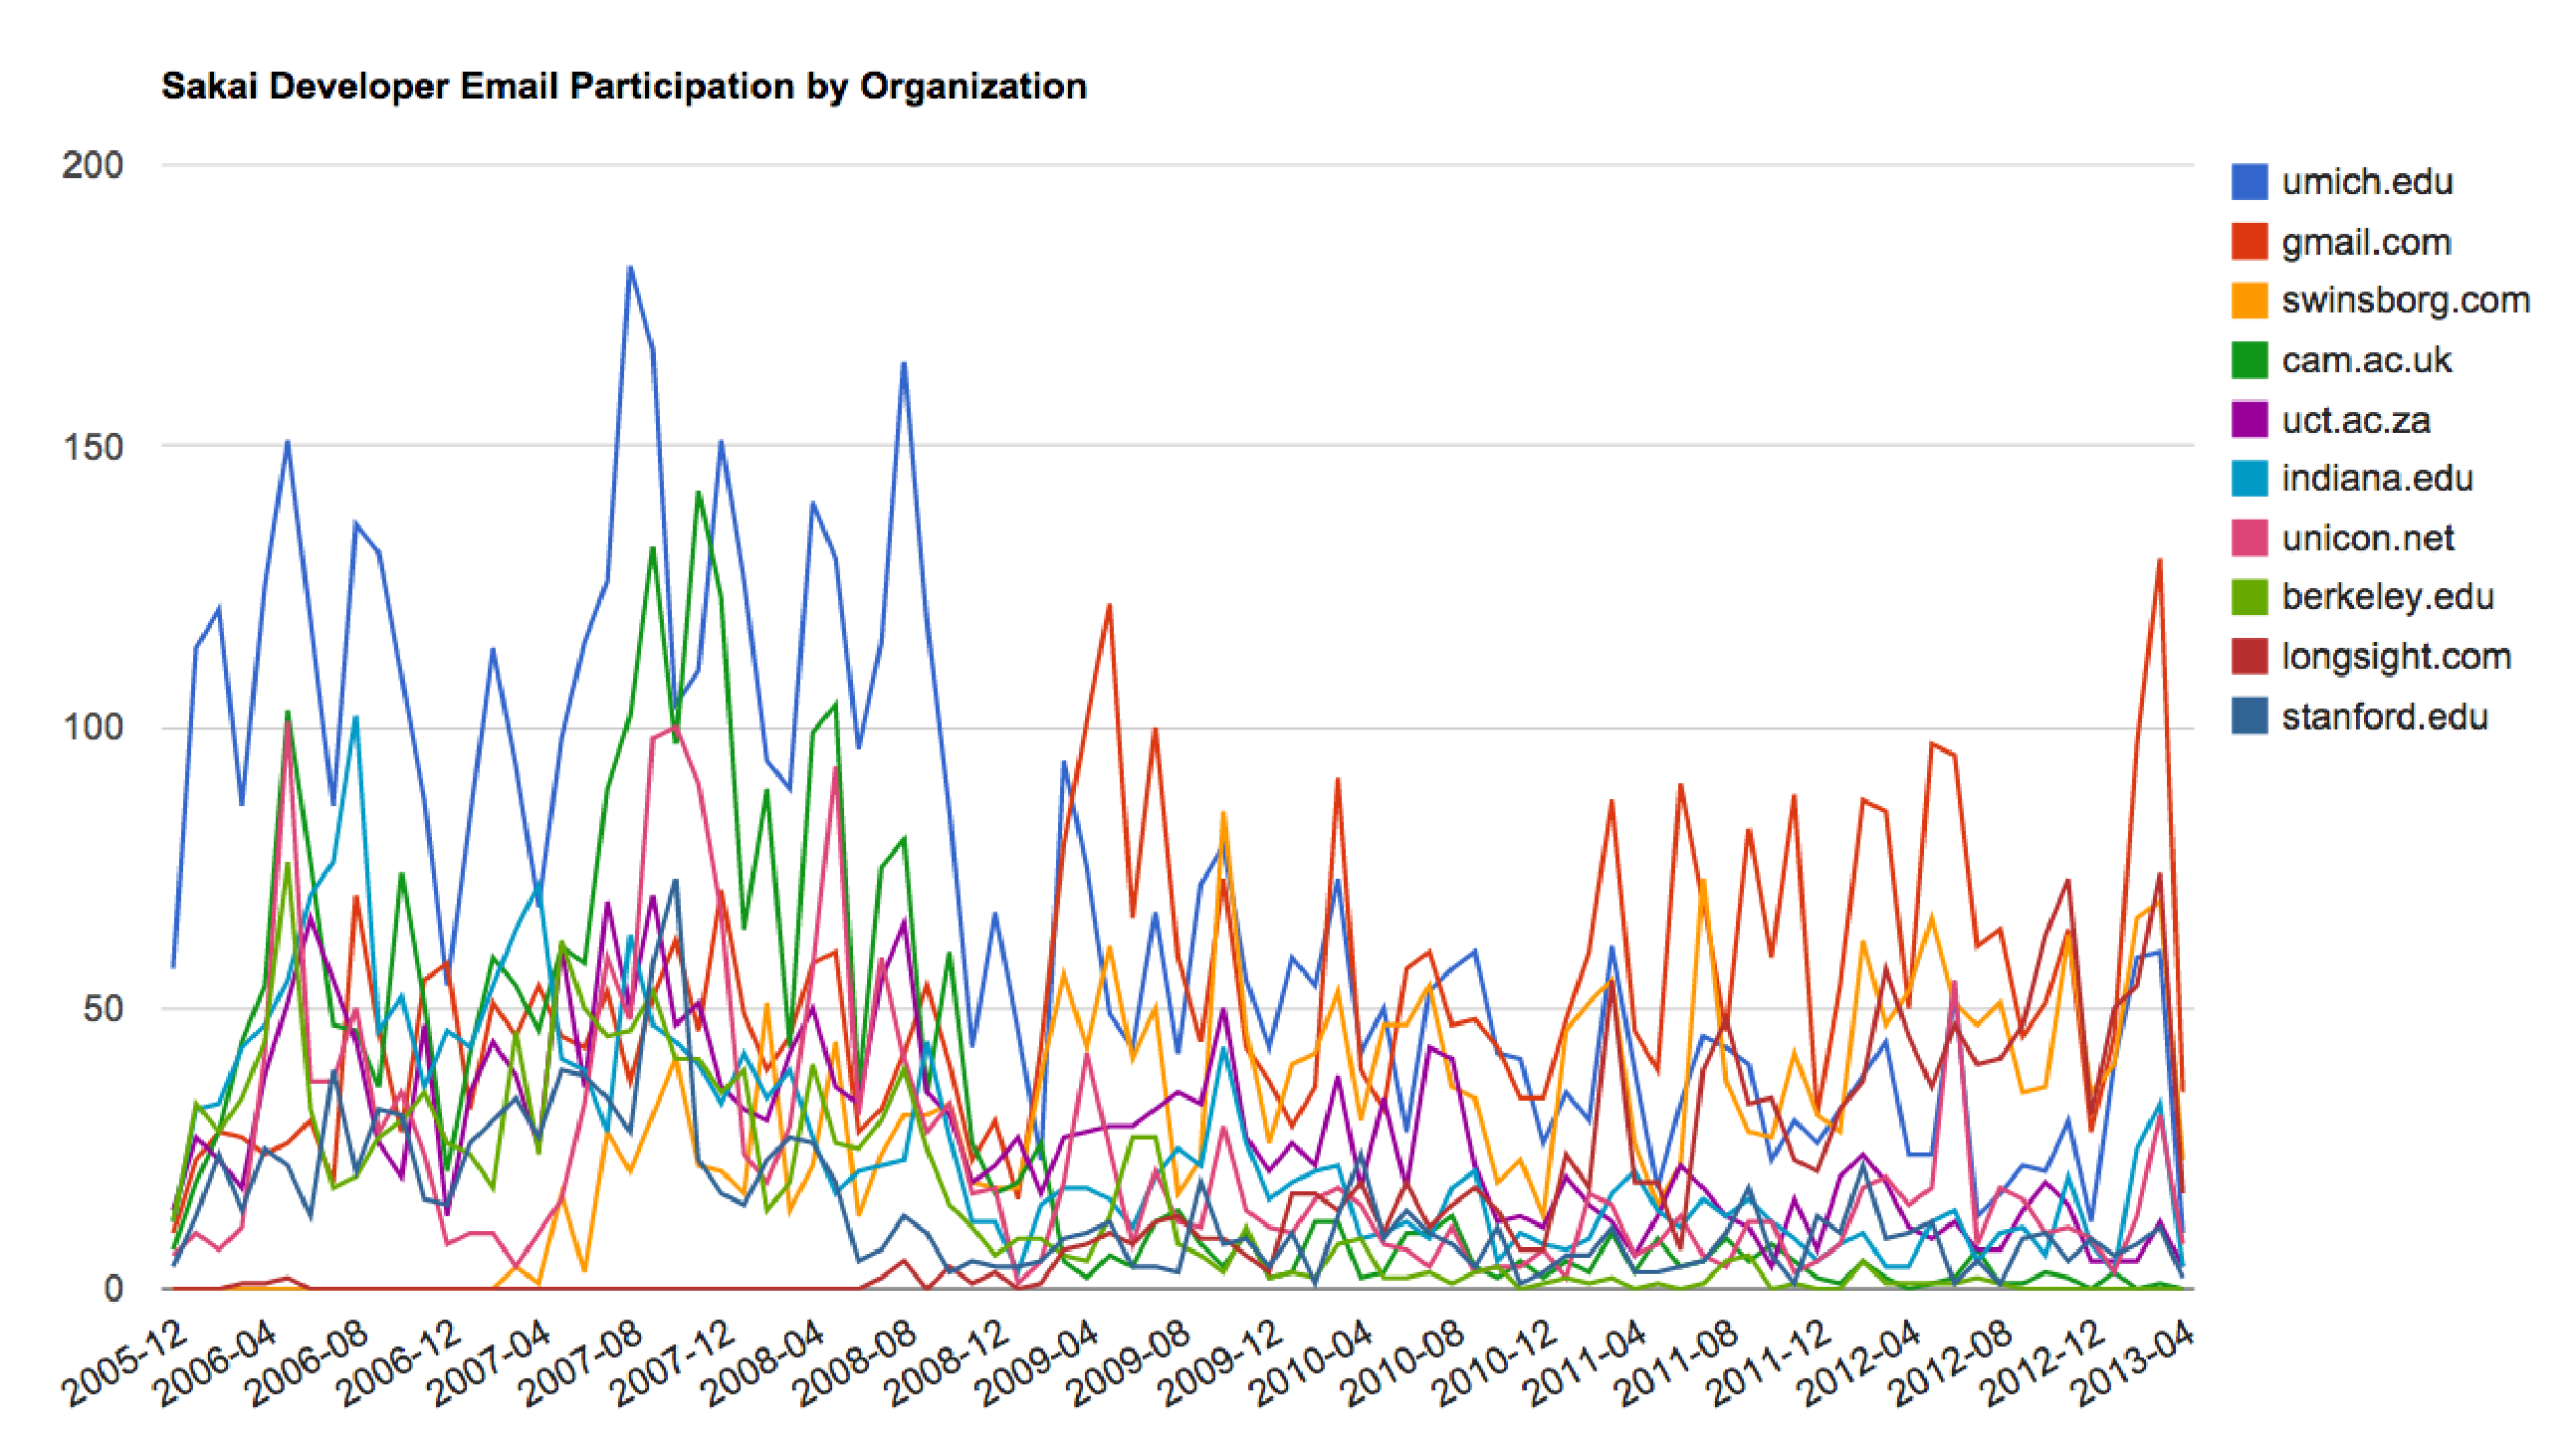
\includegraphics[keepaspectratio,alt={Sakai Mail Activity by Organization}]{../images/mailorg.eps}}
\caption{Sakai Mail Activity by Organization}
\end{figure}

Ito ay relatively complex at sophisticated application at mayroong
features para gumawa ng ilang tunay na data retrieval, cleaning, at
visualization.


\appendix

\input{tmp.appendix}

\normalsize

\printindex

% \newpage\null\thispagestyle{empty}\newpage

% \newpage\null\thispagestyle{empty}\newpage


\end{document}
